% =====================================================================
% HOL Manual LaTeX Source: tutorial
% =====================================================================

\documentclass[12pt,fleqn]{book}
%\usepackage{amsmath}
\usepackage{alltt}
\usepackage{../LaTeX/layout}
\usepackage{graphicx}
%HEVEA \usepackage{epsfig}
%PVH \usepackage{verbatim}

\renewcommand\leadsto\rightarrow

% ---------------------------------------------------------------------
% Input defined macros and commands
% ---------------------------------------------------------------------
% =====================================================================
%
% Macros for typesetting the HOL system manual
%
% =====================================================================

% ---------------------------------------------------------------------
% Abbreviations for words and phrases
% ---------------------------------------------------------------------
\newcommand\VERSION{{\small\tt 2.0}}
\newcommand\TUTORIAL{{\footnotesize\sl TUTORIAL}}
\newcommand\DESCRIPTION{{\footnotesize\sl DESCRIPTION}}
\newcommand\REFERENCE{{\footnotesize\sl REFERENCE}}
\newcommand\LIBRARIES{{\footnotesize\sl LIBRARIES}}

\def\HOL{{\small HOL}}
\def\LCF{{\small LCF}}
\def\LCFLSM{{\small LCF{\kern-.2em}{\normalsize\_}{\kern0.1em}LSM}}
\def\PPL{{\small PP}{\kern-.095em}$\lambda$}
\def\PPLAMBDA{{\small PPLAMBDA}}
\def\ML{{\small ML}}

\newcommand\ie{\mbox{i{.}e{.}}}
\newcommand\eg{\mbox{e{.}g{.}}}
\newcommand\viz{\mbox{viz{.}}}
\newcommand\adhoc{\mbox{\it ad hoc}}
\newcommand\etal{{\it et al.\/}}
\newcommand\etc{\mbox{etc{.}}}

% ---------------------------------------------------------------------
% Simple abbreviations and macros for mathematical typesetting
% ---------------------------------------------------------------------

\newcommand\fun{{\to}}
\newcommand\prd{{\times}}

\newcommand\conj{\ \wedge\ }
\newcommand\disj{\ \vee\ }
\newcommand\imp{ \Rightarrow }
\newcommand\eqv{\ \equiv\ }
\newcommand\cond{\rightarrow}
\newcommand\vbar{\mid}
\newcommand\turn{\ \vdash\ }
\newcommand\hilbert{\varepsilon}
\newcommand\eqdef{\ \equiv\ }

\newcommand\natnums{\mbox{${\sf N}\!\!\!\!{\sf N}$}}
\newcommand\bools{\mbox{${\sf T}\!\!\!\!{\sf T}$}}

\newcommand\p{$\prime$}
\newcommand\f{$\forall$\ }
\newcommand\e{$\exists$\ }

\newcommand\orr{$\vee$\ }
\newcommand\negg{$\neg$\ }

\newcommand\arrr{$\rightarrow$}
\newcommand\hex{$\sharp $}

\newcommand{\uquant}[1]{\forall #1.\ }
\newcommand{\equant}[1]{\exists #1.\ }
\newcommand{\hquant}[1]{\hilbert #1.\ }
\newcommand{\iquant}[1]{\exists ! #1.\ }
\newcommand{\lquant}[1]{\lambda #1.\ }

\newcommand{\leave}[1]{\\[#1]\noindent}
\newcommand\entails{\mbox{\rule{.3mm}{4mm}\rule[2mm]{.2in}{.3mm}}}

% ---------------------------------------------------------------------
% Font-changing commands
% ---------------------------------------------------------------------

\newcommand{\theory}[1]{\hbox{{\small\tt #1}}}

\newcommand{\con}[1]{{\sf #1}}
\newcommand{\rul}[1]{{\tt #1}}
\newcommand{\ty}[1]{{\sl #1}}

\newcommand{\ml}[1]{\mbox{{\def\_{\char'137}\small\tt #1}}}
\newcommand\ms{\tt}
\newcommand{\s}[1]{{\small #1}}

\newcommand{\pin}[1]{{\bf #1}}
\def\m#1{\mbox{\normalsize$#1$}}

% ---------------------------------------------------------------------
% Abbreviations for particular mathematical constants etc.
% ---------------------------------------------------------------------

\newcommand\T{\con{T}}
\newcommand\F{\con{F}}
\newcommand\OneOne{\con{One\_One}}
\newcommand\OntoSubset{\con{Onto\_Subset}}
\newcommand\Onto{\con{Onto}}
\newcommand\TyDef{\con{Type\_Definition}}
\newcommand\Inv{\con{Inv}}
\newcommand\com{\con{o}}
\newcommand\Id{\con{I}}
\newcommand\MkPair{\con{Mk\_Pair}}
\newcommand\IsPair{\con{Is\_Pair}}
\newcommand\Fst{\con{Fst}}
\newcommand\Snd{\con{Snd}}
\newcommand\Suc{\con{Suc}}
\newcommand\Nil{\con{Nil}}
\newcommand\Cons{\con{Cons}}
\newcommand\Hd{\con{Hd}}
\newcommand\Tl{\con{Tl}}
\newcommand\Null{\con{Null}}
\newcommand\ListPrimRec{\con{List\_Prim\_Rec}}


\newcommand\SimpRec{\con{Simp\_Rec}}
\newcommand\SimpRecRel{\con{Simp\_Rec\_Rel}}
\newcommand\SimpRecFun{\con{Simp\_Rec\_Fun}}
\newcommand\PrimRec{\con{Prim\_Rec}}
\newcommand\PrimRecRel{\con{Prim\_Rec\_Rel}}
\newcommand\PrimRecFun{\con{Prim\_Rec\_Fun}}

\newcommand\bool{\ty{bool}}
\newcommand\num{\ty{num}}
\newcommand\ind{\ty{ind}}
\newcommand\lst{\ty{list}}

% ---------------------------------------------------------------------
% \minipagewidth = \textwidth minus 1.02 em
% ---------------------------------------------------------------------

\newlength{\minipagewidth}
\setlength{\minipagewidth}{\textwidth}
\addtolength{\minipagewidth}{-1.02em}

% ---------------------------------------------------------------------
% Environment for the items on the title page of a case study
% ---------------------------------------------------------------------

\newenvironment{inset}[1]{\noindent{\large\bf #1}\begin{list}%
{}{\setlength{\leftmargin}{\parindent}%
\setlength{\topsep}{-.1in}}\item }{\end{list}\vskip .4in}

% ---------------------------------------------------------------------
% Macros for little HOL sessions displayed in boxes.
%
% Usage: (1) \setcounter{sessioncount}{1} resets the session counter
%
%        (2) \begin{session}\begin{verbatim}
%             .
%              < lines from hol session >
%             .
%            \end{verbatim}\end{session}
%
%            typesets the session in a numbered box.
% ---------------------------------------------------------------------

\newlength{\hsbw}
\setlength{\hsbw}{\textwidth}
\addtolength{\hsbw}{-\arrayrulewidth}
\addtolength{\hsbw}{-\tabcolsep}
\newcommand\HOLSpacing{13pt}

\newcounter{sessioncount}
\setcounter{sessioncount}{1}

\newenvironment{session}{\begin{flushleft}
 \begin{tabular}{@{}|c@{}|@{}}\hline
 \begin{minipage}[b]{\hsbw}
 \vspace*{-.5pt}
 \begin{flushright}
 \rule{0.01in}{.15in}\rule{0.3in}{0.01in}\hspace{-0.35in}
 \raisebox{0.04in}{\makebox[0.3in][c]{\footnotesize\sl \thesessioncount}}
 \end{flushright}
 \vspace*{-.55in}
 \begingroup\small\baselineskip\HOLSpacing}{\endgroup\end{minipage}\\ \hline
 \end{tabular}
 \end{flushleft}
 \stepcounter{sessioncount}}

% ---------------------------------------------------------------------
% Macro for boxed ML functions, etc.
%
% Usage: (1) \begin{boxed}\begin{verbatim}
%               .
%               < lines giving names and types of mk functions >
%               .
%            \end{verbatim}\end{boxed}
%
%            typesets the given lines in a box.
%
%            Conventions: lines are left-aligned under the "g" of begin,
%            and used to highlight primary reference for the ml function(s)
%            that appear in the box.
% ---------------------------------------------------------------------

\newenvironment{boxed}{\begin{flushleft}
 \begin{tabular}{@{}|c@{}|@{}}\hline
 \begin{minipage}[b]{\hsbw}
% \vspace*{-.55in}
 \vspace*{.06in}
 \begingroup\small\baselineskip\HOLSpacing}{\endgroup\end{minipage}\\ \hline
 \end{tabular}
 \end{flushleft}}

% ---------------------------------------------------------------------
% Macro for unboxed ML functions, etc.
%
% Usage: (1) \begin{hol}\begin{verbatim}
%               .
%               < lines giving names and types of mk functions >
%               .
%            \end{verbatim}\end{hol}
%
%            typesets the given lines exactly like {boxed}, except there's
%            no box.
%
%            Conventions: lines are left-aligned under the "g" of begin,
%            and used to display ML code in verbatim, left aligned.
% ---------------------------------------------------------------------

\newenvironment{hol}{\begin{flushleft}
 \begin{tabular}{c@{}@{}}
 \begin{minipage}[b]{\hsbw}
% \vspace*{-.55in}
 \vspace*{.06in}
 \begingroup\small\baselineskip\HOLSpacing}{\endgroup\end{minipage}\\
 \end{tabular}
 \end{flushleft}}

% ---------------------------------------------------------------------
% Emphatic brackets
% ---------------------------------------------------------------------

\newcommand\leb{\lbrack\!\lbrack}
\newcommand\reb{\rbrack\!\rbrack}


%These macros were included by jac1: they are used in two of the index entries

\def\per{\ml{\%}}
\def\pes{\ml{\%<}}
\def\pee{\ml{>\%}}


%These macros were included by ap; they are used in Chapters 9 and 10
%of the HOL DESCRIPTION

\newcommand{\inds}%standard infinite set
 {\mbox{\rm I}}

\newcommand{\ch}%standard choice function
 {\mbox{\rm ch}}

\newcommand{\den}[1]%denotational brackets
 {[\![#1]\!]}

\newcommand{\two}%standard 2-element set
 {\mbox{\rm 2}}













%macros for pictures in latex

\def\puthrule(#1,#2)#3{\put(#1,#2){\line(1,0){#3}}}
\def\putvrule(#1,#2)#3{\put(#1,#2){\line(0,1){#3}}}
\def\putdot(#1){\put(#1){\circle*{0.2}}}
\def\ignore#1{}
\def\putgrid(#1,#2)(#3,#4){\multiput(#1,#2)(1,0){#3}{\circle*{0.2}}
\multiput(#1,#2)(0,1){#4}{\circle*{0.2}}}

\def\putdevice(#1,#2)#3{\put(#1,#2){\framebox(4,2){\small{\tt #3}}}}
\def\putport(#1,#2)#3{\put(#1,#2){\makebox(4,1){\small{\tt #3}}}}


%\input{../LaTeX/docmacros}
\usepackage{url}
\usepackage[line,arrow,frame,matrix]{xy}
\usepackage{../LaTeX/proof}
%\includeonly{title,contents,preface,../LaTeX/ack,intro,ml,logic,
% logic-holw,proof,references,Studies/preface,Studies/parity/parity}
%             Studies/microprocessor/all,
%\includeonly{Studies/microprocessor/all}
%\includeonly{Studies/int_mod/mod_arith_study/tutorial}
%\includeonly{binomial}
%\includeonly{parity}


\begin{document}

   \setlength{\unitlength}{1mm}           % unit of length = 1mm
   \setlength{\baselineskip}{16pt}        % line spacing = 16pt

   % ---------------------------------------------------------------------
   % prelims
   % ---------------------------------------------------------------------

%   \pagenumbering{roman}                  % roman page numbers for prelims
%   \setcounter{page}{1}                   % start at page 1

%%   \typeout{}
\typeout{\space\space\space\space\space
         The title page being created is a LaTeX approximation of a fancy}
\typeout{\space\space\space\space\space
         PostScript cover page.  All the fancy cover pages for the HOL}
\typeout{\space\space\space\space\space
         Manual may be generated if you have (1) a PostScript printer,}
\typeout{\space\space\space\space\space
         (2) the "psfig" TeX macros, and (3) a DVI to PostScript converter}
\typeout{\space\space\space\space\space
         that understands these macros.  The cover pages may be found in}
\typeout{\space\space\space\space\space
         ../LaTeX/Covers, and shoud be made pursuant to the instructions}
\typeout{\space\space\space\space\space
         given in ../LaTeX/Covers/READ-ME.}
\typeout{}




\begin{titlepage}
\null\vskip-47pt
\hbox to \textwidth {\bf [For \holn{} Taupo-2]  {\hfil \today}}

\setcounter{page}{1}                      % titlepage IS page 1

\vspace*{60mm}


\begin{center}
 {\Huge\bf The HOL System}\\[0.4cm]
{\LARGE\bf REFERENCE}\\[2.5cm]
\end{center}

\vspace*{100mm}
\begin{center}
\begin{tabular}{ccc}
University of Cambridge & \hspace*{10ex}DSTO\hspace*{10ex} & SRI International
\end{tabular}
\end{center}

\vfill
\end{titlepage}

% To kick a blank page with no header
\thispagestyle{empty}
\mbox{}
\newpage

%%% Local Variables:
%%% mode: latex
%%% TeX-master: "reference"
%%% End:
                        % tutorial title page
   \begin{titlepage}
\null\vskip-47pt
\hbox to \textwidth
{\bf [For \holnw{} \holnversion] { \hfil \today}}

\setcounter{page}{1}                      % titlepage IS page 1

\vspace*{60mm}


{\fontfamily{ptm}\selectfont
\begin{center}
\scalebox{1.4}{\begin{tabular}{c} \Huge The HOL-Omega System \\[4pt] \huge TUTORIAL TEASER \end{tabular}} \\
\end{center}}

\begin{center}
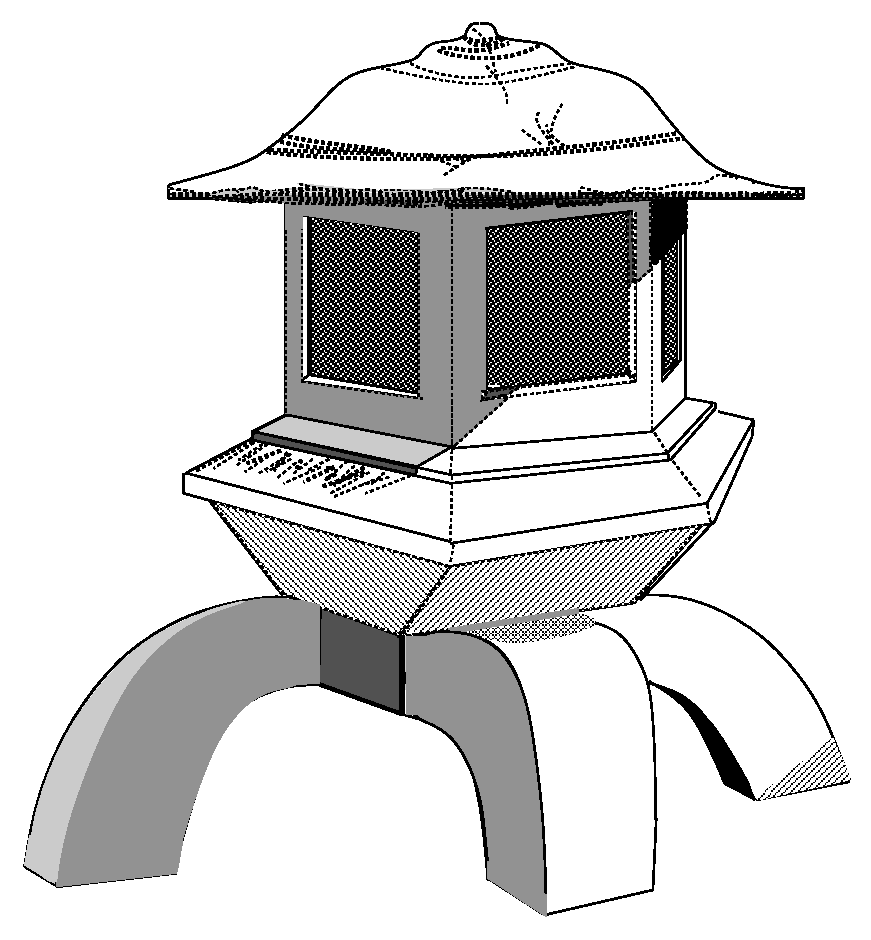
\includegraphics[width=3.8cm]{../Logo/lantern}
\end{center}


\vfill
\end{titlepage}

% To kick a blank page with no header
\thispagestyle{empty}
\cleardoublepage

%END LATEX

%HEVEA \begin{tabular}{l@{\hspace{5cm}}r}
%HEVEA {\bf [For \holnw{} \holnversion]} & \today\\
%HEVEA \end{tabular}
%HEVEA
%HEVEA \begin{center}
%HEVEA {\Huge\bf The HOL-Omega System}\\
%HEVEA {\LARGE \bf TUTORIAL TEASER}\\
%HEVEA \vspace{1cm}
%HEVEA \begin{toimage}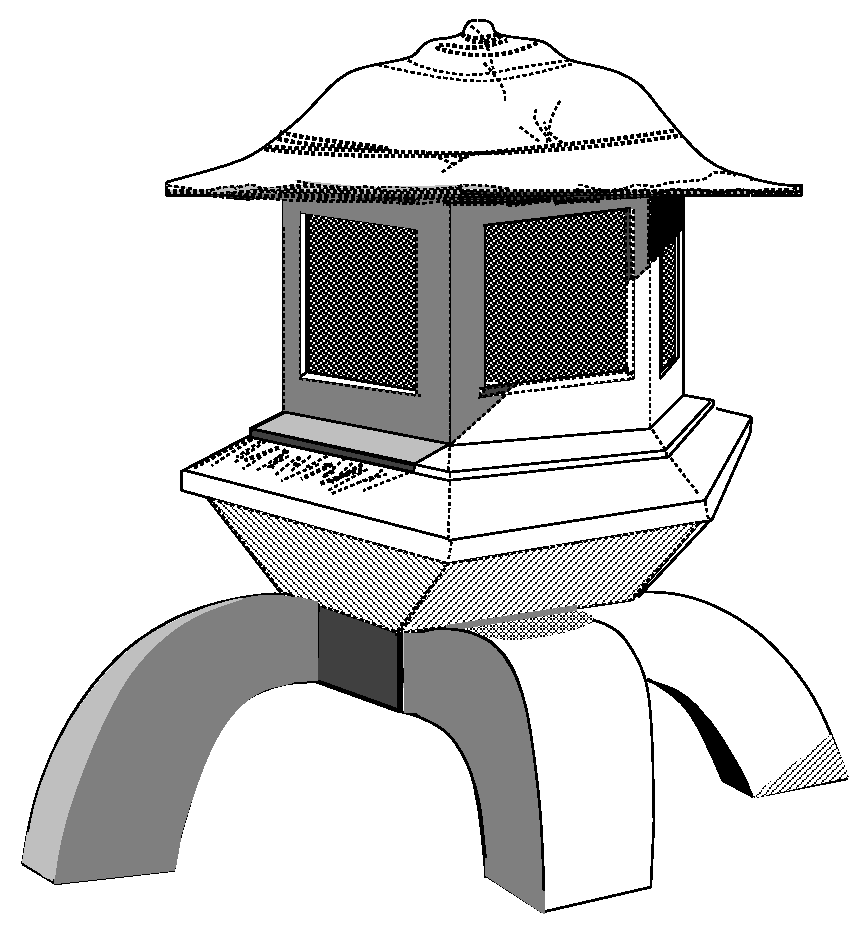
\epsfig{file=../Covers/LANTERN.ps,height=2.5in}\\
%HEVEA \end{toimage}\imageflush
%HEVEA \begin{tabular}{ccc}
%HEVEA University of Cambridge & \hspace*{10ex}DSTO\hspace*{10ex} & SRI International
%HEVEA \end{tabular}
%HEVEA \end{center}




%%% Local Variables:
%%% mode: latex
%%% TeX-master: "tutorial"
%%% End:
                  % tutorial teaser title page
%%   \chapter*{Preface}\markboth{Preface}{Preface}

This volume is the reference manual for the \HOL\ system.
It is one of four documents making up the documentation for \HOL:

\begin{myenumerate}
\item \LOGIC: a formal description of the higher order logic
  implemented by the \HOL{} system.
\item \TUTORIAL: a tutorial introduction to \HOL, with case studies.
\item \DESCRIPTION: a detailed user's guide for the \HOL{} system;
\item \REFERENCE: the reference manual for \HOL.
\end{myenumerate}

\noindent These four documents will be referred to by the short names (in
small slanted capitals) given above.

This document, \REFERENCE, provides documentation on all the pre-defined \ML\
variable bindings in the \HOL\ system.  These include: general-purpose
functions, such as \ML\ functions for list processing, arithmetic,
input/output, and interface configuration; functions for processing the types
and terms of the \HOL\ logic, for setting up theories, and for using the
subgoal package; primitive and derived forward inference rules; tactics and
tacticals; and pre-proved built-in theorems.

% The manual entries for these \ML\ identifiers are divided into two chapters.
% The first chapter is an alphabetical sequence of manual entries for all \ML\
% identifiers in the system except those identifiers that are bound to theorems.
% The theorems are listed in the second chapter, roughly grouped into sections
% based on subject matter.

The \REFERENCE\ volume is purely for reference and browsing. It is generated
from the same database that is used by the help system. For an introduction to
the \HOL\ system, see \TUTORIAL; for a systematic presentation, see
\DESCRIPTION{}  and \LOGIC{}.
                      % preface to entire tutorial
   \chapter*{Prologue}\markboth{Prologue}{Prologue}
\label{prologue}

This volume contains a short sample of material from the upcoming
tutorial on the \HOLW{} system.  The tutorial will be one of four
documents making up the documentation for \HOLW:

\begin{myenumerate}
\item \LOGIC: a formal description of the higher order logic
  implemented by the \HOLW{} system.
\item \TUTORIAL: a tutorial introduction to \HOLW, with case studies.
\item \DESCRIPTION: a detailed user's guide for the \HOLW{} system;
\item \REFERENCE: the reference manual for \HOLW.
\end{myenumerate}

This document provides a brief and light set of examples of using \HOLW{},
as an introduction, giving a taste of how the system might be used.
Like an appetizer to a main meal, it provides just a hint of
the sustenance to come.

\section*{Getting started}

Chapter~\ref{install} explains how to get and install \HOLW.
Then the new, additional
concepts and features of the \HOLW{} logic (higher order logic 
extended with System {\it F}, kinds, and ranks)
are casually demonstrated,
in chapter \ref{chap:appetizers}.

Chapter~\ref{chap:teaser_epilogue} briefly discusses some of the
examples distributed with \holnw{} in the \ml{examples/HolOmega} directory.

%\item Chapter~\ref{tool} shows how a special purpose proof tool (a
%  conjunction normaliser) can be implemented and optimised. It
%  illustrates methods for `tuning' proof generating programs and
%  discusses trade-offs between generality and efficiency.

%\item Chapter~\ref{binomial} is a proof of the Binomial Theorem in a
%  ring.  It is a medium sized worked example whose subject matter is
%  probably more widely known than any specific piece of hardware or
%  software. The small amount of algebra and mathematical notation
%  needed to state and prove the Binomial Theorem is presented; the
%  notation is expressed in \HOLW{}, and the structure of the proof is
%  outlined.

%\end{itemize}

\vspace{1cm}

%\noindent \TUTORIAL{} has been kept short so that new users of \HOLW{} can get
%going as fast as possible. Sometimes details have been simplified. It
%is recommended that as soon as a topic in \TUTORIAL\ has been
%digested, the relevant parts of \DESCRIPTION\ and \REFERENCE\ be
%studied.

%%% Local Variables:
%%% mode: latex
%%% TeX-master: "tutorial"
%%% End:
                      % prologue to teaser
   \chapter*{Acknowledgements}\markboth{Acknowledgements}{Acknowledgements}

The bulk of \HOL\ is based on code written by---in alphabetical
order---Hasan Amjad, Richard Boulton, Anthony Fox, Mike Gordon, Elsa
Gunter, John Harrison, Peter Homeier, G\'erard Huet (and others at
INRIA), Joe Hurd, Ken Larsen, Tom Melham, Robin Milner, Lockwood
Morris, Magnus Myreen, Malcolm Newey, Michael Norrish, Larry Paulson,
Konrad Slind, Don Syme, Thomas T\"urk, Chris Wadsworth, and Tjark
Weber.  Many others have supplied parts of the system, bug fixes, etc.

\subsection*{Current edition}

The current edition of all four volumes (\LOGIC, \TUTORIAL,
\DESCRIPTION\ and \REFERENCE) has been prepared by Michael Norrish and
Konrad Slind. Further contributions to these volumes came from: Hasan
Amjad, who developed a model checking library and wrote sections
describing its use; Jens Brandt, who developed and documented a
library for the rational numbers; Anthony Fox, who formalized and
documented new word theories and the associated libraries; Mike
Gordon, who documented the libraries for BDDs and SAT; Peter Homeier,
who implemented and documented the quotient library; Joe Hurd, who
added material on first order proof search; and Tjark Weber, who wrote
libraries for Satisfiability Modulo Theories~(SMT) and Quantified
Boolean Formulae~(QBF).

\medskip

The material in the third edition constitutes a thorough re-working
and extension of previous editions.  The only essentially unaltered
piece is the semantics by Andy Pitts (in \LOGIC), reflecting the fact
that, although the \HOL\ system has undergone continual development
and improvement, the \HOL\ logic is unchanged since the first edition
(1988).

\newpage

\subsection*{Second edition}

The second edition of \REFERENCE\ was a joint effort by the Cambridge
\HOL\ group.

\subsection*{First edition}

The three volumes \TUTORIAL, \DESCRIPTION\ and \REFERENCE\ were
produced at the Cambridge Research Center of SRI International with
the support of DSTO Australia.

The \HOL\ documentation project was managed by Mike Gordon, who also
wrote parts of \DESCRIPTION\ and \TUTORIAL\ using material based on an
early paper describing the \HOL\ system\footnote{M.J.C.\ Gordon, `HOL:
  a Proof Generating System for Higher Order Logic', in: {\it VLSI
    Specification, Verification and Synthesis\/}, edited by G.\
  Birtwistle and P.A.\ Subrahmanyam, (Kluwer Academic Publishers,
  1988), pp.\ 73--128.} and {\sl The ML Handbook\/}\footnote{{\sl The
    ML Handbook}, unpublished report from Inria by Guy Cousineau, Mike
  Gordon, G\'erard Huet, Robin Milner, Larry Paulson and Chris
  Wadsworth.}.  Other contributers to \DESCRIPTION\ incude Avra Cohn,
who contributed material on theorems, rules, conversions and tactics,
and also composed the index (which was typeset by Juanito Camilleri);
Tom Melham, who wrote the sections describing type definitions, the
concrete type package and the `resolution' tactics; and Andy Pitts,
who devised the set-theoretic semantics of the \HOL\ logic and wrote
the material describing it.

The original document design used \LaTeX\ macros supplied by Elsa
Gunter, Tom Melham and Larry Paulson.  The typesetting of all three
volumes was managed by Tom Melham.  The cover design is by Arnold
Smith, who used a photograph of a `snow watching lantern' taken by
Avra Cohn (in whose garden the original object resides).  John Van
Tassel composed the \LaTeX\ picture of the lantern.

Many people other than those listed above have contributed to the
\HOL\ documentation effort, either by providing material, or by
sending lists of errors in the first edition.  Thanks to everyone who
helped, and thanks to DSTO and SRI for their generous support.






                 % global acknowledgements
   \tableofcontents

%   \newpage
%   \pagenumbering{arabic}                % arabic page numbers
%   \setcounter{page}{1}                  % start at page 1

   \chapter{Getting and Installing \HOL{}}
\label{install}

This chapter describes how to get the \HOL{} system and how to install
it.  It is generally assumed that some sort of Unix system is being
used, but the instructions that follow should apply {\it mutatis
  mutandis\/} to other platforms.  Unix is not a pre-requisite for
using the system. \HOL{} may be run on PCs running Windows operating
systems from Windows~NT onwards (i.e., Windows~2000, XP and Vista are
also supported), as well as Macintoshes running MacOS~X.

\section{Getting \HOL{}}

The \HOL{} system can be downloaded from
\url{http://hol.sourceforge.net}.  The naming scheme for \holn{}
releases is $\langle${\it name}$\rangle$-$\langle${\it
  number}$\rangle$; the release described here is \holnversion.

\section{The {\tt hol-info} mailing list}

The \texttt{hol-info} mailing list serves as a forum for discussing
\HOL{} and disseminating news about it.  If you wish to be on this
list (which is recommended for all users of \HOL), visit
\url{http://lists.sourceforge.net/lists/listinfo/hol-info}.  This
web-page can also be used to unsubscribe from the mailing list.

\section{Installing \HOL{}}

It is assumed that the \HOL{} sources have been obtained and the
\texttt{tar} file unpacked into a directory \ml{hol}.\footnote{You may
  choose another name if you want; it is not important.} The contents
of this directory are likely to change over time, but it should
contain the following:

\begin{center}
\begin{tabular}{|l|l|l|} \hline
\multicolumn{3}{|c|}{ } \\
\multicolumn{3}{|c|}{\bf Principal Files on the HOL Distribution Directory} \\
\multicolumn{3}{|c|}{ } \\
{\it File name} & {\it Description} & {\it File type}  \\ \hline
{\tt README} & Description of directory {\tt hol} & Text\\
{\tt COPYRIGHT}& A copyright notice & Text\\
{\tt INSTALL} & Installation instructions & Text\\
{\tt tools} & Source code for building the system & Directory\\
{\tt bin} & Directory for HOL executables & Directory\\
{\tt sigobj} & Directory for \ML{} object files & Directory\\
{\tt src} & \ML{} sources of \HOL & Directory\\
{\tt help} & Help files for \HOL{} system & Directory\\
{\tt examples} & Example source files & Directory\\
\hline
\end{tabular}
\end{center}

The session in the box below shows a typical distribution directory.
The \HOL{} distribution has been placed on a PC running Linux in the
directory {\small\tt /home/mn200/hol/}.

All sessions in this documentation will be displayed in boxes with a
number in the top right hand corner.  This number indicates whether
the session is a new one (when the number will be {\small\sl 1}) or
the continuation of a session started in an earlier box.
Consecutively numbered boxes are assumed to be part of a single
continuous session.  The Unix prompt for the sessions is
\texttt{\small \dol}, so lines beginning with this prompt were typed
by the user.  After entering the \HOL{} system (see below), the user
is prompted with {\small\verb|-|} for an expression or command of the
\HOL{} meta-language \ML; lines beginning with this are thus \ML\
expressions or declarations.  Lines not beginning with \texttt{\small
  \$} or {\small\verb|-|} are system output.  Occasionally, system
output will be replaced with a line containing {\small\verb|...|} when
it is of minimal interest. The meta-language \ML{} is introduced in
Chapter~\ref{ML}.

\setcounter{sessioncount}{0}
\begin{session}
\begin{verbatim}
$ pwd
/home/mn200/hol
$ ls -F
COPYRIGHT  bin/  examples/  INSTALL  src/
README     doc/  help/      sigobj/  tools/
\end{verbatim}
\end{session}

Now you will need to rebuild \HOL{} from the sources.\footnote{It is
  possible that pre-built systems may soon be available from the
  web-page mentioned above.}

Before beginning you must have a current version of Moscow~ML or
Poly/ML\footnote{Poly/ML cannot be used with HOL on Windows.}.  In the
case of Moscow~ML, you must have version 2.01.  Moscow~ML is available
on the web from \url{http://www.itu.dk/~sestoft/mosml.html}.
Poly/ML is available from \url{http://polyml.org}.

When working with Poly/ML, the installation must ensure that dynamic library loading (typically done by setting the \texttt{LD\_LIBRARY\_PATH} environment variable) picks up \texttt{libpolyml.so} and \texttt{libpolymain.so}.
If these files are in \texttt{/usr/lib}, nothing will need to be changed, but other locations may require further system configuration.
A sample \texttt{LD\_LIBRARY\_PATH} initialisation command (in a file such as \texttt{.bashrc}) might be
\begin{verbatim}
   declare -x LD_LIBRARY_PATH=/usr/local/lib:$HOME/lib
\end{verbatim}
Further, if you are using Poly/ML version 5.5.1 or later, you will need to make sure that Poly/ML is configured with the \texttt{--enable-shared} option.
That is, your configure command (the first thing that is done when building the system), will look something like
\begin{verbatim}
   ./configure --enable-shared
\end{verbatim}

When you have your ML system installed, and are in the root directory of the distribution, the next step is to run \texttt{smart-configure}.
With Moscow~ML, this looks like:

\begin{session}
\begin{alltt}
\dol mosml < tools/smart-configure.sml
Moscow ML version 2.01 (January 2004)
Enter `quit();' to quit.
- [opening file "tools/smart-configure-mosml.sml"]

HOL smart configuration.

Determining configuration parameters: OS mosmldir holdir
OS:                 linux
mosmldir:           /home/mn200/mosml/bin
holdir:             /home/mn200/hol
dynlib_available:   true

Configuration will begin with above values.  If they are wrong
press Control-C.
\end{alltt}
\end{session}

If you are using Poly/ML, then write
\begin{verbatim}
   poly < tools/smart-configure.sml
\end{verbatim}
instead.

Assuming you don't interrupt the configuration process, this will
build the \texttt{Holmake} and \texttt{build} programs, and move them
into the \texttt{hol/bin} directory.  If something goes wrong at this
stage, consult Section~\ref{sec:editting-configure} below.

The next step is to run the \texttt{build} program.  This should
result in a great deal of output as all of the system code is compiled
and the theories built.  Eventually, a \HOL{} system\footnote{Four
  \HOL{} executables are produced: \textsf{hol}, \textsf{hol.noquote},
  \textsf{hol.bare} and \textsf{hol.bare.noquote}.  The first of these
  will be used for most examples in the \TUTORIAL{}.} is produced in
the \texttt{bin/} directory.

\begin{session}
\begin{alltt}
\dol bin/build
  ...
  ...
Uploading files to /home/mn200/hol/sigobj

Hol built successfully.
\dol
\end{alltt}
\end{session}


\subsection{Overriding \texttt{smart-configure}}
\label{sec:editting-configure}

If \texttt{smart-configure} is unable to guess correct values for the
various parameters (\texttt{holdir}, \texttt{OS} \etc) then you can
create a file called to provide correct values.  With Moscow~ML, this
should be \texttt{config-override} in the root directory of the HOL
distribution.  With Poly/ML, this should be \texttt{poly-includes.ML}
in the \texttt{tools-poly} directory. In this file, specify the
correct value for the appropriate parameter by providing an ML binding
for it.  All variables except \texttt{dynlib\_available} must be given
a string as a possible value, while \texttt{dynlib\_available} must be
either \texttt{true} or \texttt{false}.  So, one might write

\begin{session}
\begin{verbatim}
val OS = "unix";
val holdir = "/local/scratch/myholdir";
val dynlib_available = false;
\end{verbatim}
\end{session}

The \texttt{config-override} file need only provide values for those
variables that need overriding.

With this file in place, the \texttt{smart-configure} program will use
the values specified there rather than those it attempts to calculate
itself.  The value given for the \texttt{OS} variable must be one of
\texttt{"unix"}, \texttt{"linux"}, \texttt{"solaris"},
\texttt{"macosx"} or \texttt{"winNT"}.\footnote{The string
  \texttt{"winNT"} is used for Microsoft Windows operating systems
  that are at least as recent as Windows~NT.  This includes
  Windows~2000, XP and Vista.}

In extreme circumstances it is possible to edit the file
\texttt{tools/configure.sml} yourself to set configuration variables
directly.  (If you are using Poly/ML, you must edit
\texttt{tools-poly/configure.sml} instead.) At the top of this file
various incomplete SML declarations are present, but commented out.
You will need to uncomment this section (remove the \texttt{(*} and
\texttt{*)} markers), and provide sensible values.  All strings must
be enclosed in double quotes.

The \texttt{holdir} value must be the name of the top-level directory
listed in the first session above.  The \texttt{OS} value should be
one of the strings specified in the accompanying comment.

When working with Moscow~ML, the \texttt{mosmldir} value must be the
name of the directory containing the Moscow~ML binaries
(\texttt{mosmlc}, \texttt{mosml}, \texttt{mosmllex} etc).  When
working with Poly/ML, the \texttt{poly} string must be the path to the
\texttt{poly} executable that begins an interactive \ML{} session.
The \texttt{polymllibdir} must be a path to a directory that contains
the file \texttt{libpolymain.a}.

Subsequent values (\texttt{CC} and \texttt{GNUMAKE}) are needed for
``optional'' components of the system.  The first gives a string
suitable for invoking the system's C compiler, and the second
specifies a \textsf{make} program.

After editing, \texttt{tools/configure.sml} the lines above will look
something like:

\begin{session}
\begin{alltt}
\dol more configure.sml
  ...
val mosmldir = "/home/mn200/mosml";
val holdir   = "/home/mn200/hol";
val OS       = "linux"       (* Operating system; choices are:
                                "linux", "solaris", "unix", "winNT" *)

val CC       = "gcc";     (* C compiler (for building quote filter)        *)
val GNUMAKE  = "gnumake"; (* for robdd library                             *)
  ...
\dol
\end{alltt}
\end{session}

\noindent Now, at either this level (in the \texttt{tools} or
\texttt{tools-poly} directory) or at the level above, the script
\texttt{configure.sml} must be piped into the \ML{} interpreter (\ie,
\texttt{mosml} or \texttt{poly}).  For example,

\begin{session}
\begin{alltt}
\dol mosml < tools/configure.sml
Moscow ML version 2.01 (January 2004)
Enter `quit();' to quit.
- > val mosmldir = "/home/mn200/mosml" : string
  val holdir = "/home/mn200/hol" : string
  val OS = "linux" : string
- > val CC = "gcc" : string
  ...
Beginning configuration.
- Making bin/Holmake.
  ...
Making bin/build.
- Making hol98-mode.el (for Emacs)
- Setting up the standard prelude.
- Setting up src/0/Globals.sml.
- Generating bin/hol.
- Generating bin/hol.noquote.
- Attempting to compile quote filter ... successful.
- Setting up the muddy library Makefile.
- Setting up the help Makefile.
-
Finished configuration!
-
\dol
\end{alltt}
\end{session}



%%% Local Variables:
%%% mode: latex
%%% TeX-master: "tutorial"
%%% End:
                       % intro: getting and installing hol
%%   \chapter{Introduction to ML}
\label{ML}

This chapter is a brief introduction to the meta-language \ML.  The
aim is just to give a feel for what it is like to interact with the
language.  A more detailed introduction can be found in numerous
textbooks and web-pages; see for example the list of resources on the
\url{http://www.dina.kvl.dk/\~{}sestoft/mosml.html}{MoscowML home-page},
or the
\url{http://src.doc.ic.ac.uk/usenet/news-faqs/comp.lang.ml/}{\texttt{comp.lang.ml} FAQ}.

\section{How to interact with ML}

\ML{} is an interactive programming language like Lisp. At top level
one can evaluate expressions and perform declarations. The former
results in the expression's value and type being printed, the latter
in a value being bound to a name.

A standard way to interact with \ML{} is to configure the workstation
screen so that there are two windows:
\begin{myenumerate}
\item An editor window into which \ML{} commands are initially typed
  and recorded.
\item A shell window (or non-Unix equivalent) which is used to
  evaluate the commands.
\end{myenumerate}

\noindent
A common way to achieve this is to work inside \ml{Emacs} with a text
window and a shell window.

After typing a command into the edit (text) window it can be
transferred to the shell and evaluated in \HOL{} by `cut-and-paste'. In
\ml{Emacs} this is done by copying the text into a buffer and then
`yanking' it into the shell. The advantage of working via an editor is
that if the command has an error, then the text can simply be edited
and used again; it also records the commands in a file which can then
be used again (via a batch load) later. In \ml{Emacs}, the shell
window also records the session, including both input from the user
and the system's response. The sessions in this tutorial were produced
this way. These sessions are split into segments displayed in boxes
with a number in their top right hand corner (to indicate their
position in the complete session).

The interactions in these boxes should be understood as occurring in
sequence.  For example, variable bindings made in earlier boxes are
assumed to persist to later ones.  To enter the \HOL{} system one types
{\small\verb|hol|} or {\small\verb|hol.unquote|} to Unix, possibly
  preceded by path information if the \HOL{} system's \texttt{bin}
  directory is not in one's path.  The \HOL{} system then prints a
  sign-on message and puts one into \ML.  The \ML{} prompt is
  {\small\verb|-|}, so lines beginning with {\small\verb|-|} are typed
  by the user and other lines are the system's responses.

  Here, as elsewhere in the \TUTORIAL{}, we will be assuming use of
  {\small\verb|hol.unquote|}.

\setcounter{sessioncount}{1}
\begin{session}\begin{alltt}
\$ bin/hol.unquote
Moscow ML version 1.44 (August 1999)
Enter `quit();' to quit.

-----------------------------------------------------------
           HOL98 [Taupo 3]

   For introductory HOL help, type: help "hol";
-----------------------------------------------------------

[closing file "/local/scratch/mn200/Work/hol98/tools/end-init.sml"]
- 1 :: [2,3,4,5];
> val it = [1, 2, 3, 4, 5] : int list
\end{alltt}
\end{session}

The \ML{} expression {\small\verb|1 :: [2,3,4,5]|} has the form $e_1\
op\ e_2$ where $e_1$ is the expression {\small\verb|1|} (whose value
is the integer $1$), $e_2$ is the expression {\small\verb|[2,3,4,5]|}
(whose value is a list of four integers) and $op$ is the infixed
operator `{\small\verb|::|}' which is like Lisp's {\it cons} function.
Other list processing functions include {\small\verb|hd|} ($car$ in
Lisp), {\small\verb|tl|} ($cdr$ in Lisp) and {\small\verb|null|}
($null$ in Lisp).  The semicolon `{\small\verb|;|}' terminates a
top-level phrase.  The system's response is shown on the line starting
with the {\small\verb|>|} prompt.  It consists of the value of the
expression followed, after a colon, by its type. The \ML{} type checker
infers the type of expressions using methods invented by Robin Milner
\cite{Milner-types}. The type {\small\verb|int list|} is the type of
`lists of integers'; {\small\verb|list|} is a unary type operator.
The type system of \ML{} is very similar to the type system of the
\HOL{} logic which is explained in Chapter~\ref{HOLlogic}.

The value of the last expression evaluated at top-level in \ML{} is always
remembered in a variable called {\small\verb|it|}.

\begin{session}
\begin{verbatim}
- val l = it;
> val l = [1, 2, 3, 4, 5] : int list

- tl l;
> val it = [2, 3, 4, 5] : int list

- hd it;
> val it = 2 : int

- tl(tl(tl(tl(tl l))));
> val it = [] : int list
\end{verbatim}
\end{session}

Following standard $\lambda$-calculus usage, the application of a
function $f$ to an argument $x$ can be written without brackets as $f\
x$ (although the more conventional
$f${\small\verb|(|}$x${\small\verb|)|} is also allowed).  The
expression $f\ x_1\ x_2\ \cdots\ x_n$ abbreviates the less
intelligible expression {\small\verb|(|}$\cdots${\small\verb|((|}$f\ x_1$%
{\small\verb|)|}$x_2${\small\verb|)|}$\cdots${\small\verb|)|}$x_n$
(function application is left associative).

Declarations have the form {\small\verb|val |}$x_1${\small\verb|=|}$e_1${\small\verb| and |}$\cdots
${\small\verb| and |}$x_n${\small\verb|=|}$e_n$ and result in the value of
each expression $e_i$ being bound to the name $x_i$.

\begin{session}
\begin{verbatim}
- val l1 = [1,2,3] and l2 = ["a","b","c"];
> val l1 = [1, 2, 3] : int list
  val l2 = ["a", "b", "c"] : string list
\end{verbatim}
\end{session}

\ML{} expressions like {\small\verb|"a"|}, {\small\verb|"b"|},
{\small\verb|"foo"|} \etc\ are {\it strings\/} and have type
{\small\verb|string|}. Any sequence of {\small ASCII} characters can
be written between the quotes.\footnote{Newlines must be written as
  \ml{$\backslash$n}, and quotes as \ml{$\backslash$"}.} The function
{\small\verb|explode|} splits a string into a list of single
characters, which are written like single character strings, with a
{\small\verb|#|} character prepended.

\begin{session}
\begin{verbatim}
- explode "a b c";
> val it = [#"a", #" ", #"b", #" ", #"c"] : char list
\end{verbatim}
\end{session}

An expression of the form
{\small\verb|(|}$e_1${\small\verb|,|}$e_2${\small\verb|)|} evaluates
to a pair of the values of $e_1$ and $e_2$. If $e_1$ has type
$\sigma_1$ and $e_2$ has type $\sigma_2$ then
{\small\verb|(|}$e_1${\small\verb|,|}$e_2${\small\verb|)|} has type
$\sigma_1${\small\verb|*|}$\sigma_2$.  The first and second components
of a pair can be extracted with the \ML{} functions {\small\verb|#1|}
and {\small\verb|#2|} respectively.  If a tuple has more than two
components, its $n$-th component can be extracted with a function
{\small\verb|#|$n$}.

The values {\small\verb|(1,2,3)|}, {\small\verb|(1,(2,3))|} and
{\small\verb|((1,2), 3)|} are all distinct and have types
\linebreak{} {\small\verb|int * int * int|}, {\small\verb|int * (int * int)|} and
{\small\verb|(int * int) * int|} respectively.

\begin{session}
\begin{verbatim}
- val triple1 = (1,true,"abc");
> val triple1 = (1, true, "abc") : int * bool * string
- #2 triple1;
> val it = true : bool

- val triple2 = (1, (true, "abc"));
> val triple2 = (1, (true, "abc")) : int * (bool * string)
- #2 triple2;;
> val it = (true, "abc") : bool * string
\end{verbatim}
\end{session}

\noindent The \ML{} expressions {\small\verb|true|} and {\small\verb|false|}
denote the two truth values of type {\small\verb|bool|}.

\ML{} types can contain the {\it type variables\/} {\small\verb|'a|},
{\small\verb|'b|}, {\small\verb|'c|}, \etc\ Such types are called {\it
polymorphic\/}. A function with a polymorphic type should be thought of as
possessing all the types obtainable by replacing type variables by types.
This is illustrated below with the function {\small\verb|zip|}.

Functions are defined with declarations of the form {\small\verb|fun|}$\ f\
v_1\ \ldots\ v_n$ \ml{=} $e$ where each $v_i$ is either a variable or a pattern
built out of variables.

The function {\small\verb|zip|}, below, converts a pair of lists
{\small\verb|([|}$x_1${\small\verb|,|}$\ldots${\small\verb|,|}$x_n$%
{\small\verb|], [|}$y_1${\small\verb|,|}$\ldots${\small\verb|,|}$y_n$%
{\small\verb|])|} to a list of pairs
{\small\verb|[(|}$x_1${\small\verb|,|}$y_1${\small\verb|),|}$\ldots$%
{\small\verb|,(|}$x_n${\small\verb|,|}$y_n${\small\verb|)]|}.

\begin{session}
\begin{verbatim}
- fun zip(l1,l2) =
    if null l1 orelse null l2 then []
    else (hd l1,hd l2) :: zip(tl l1,tl l2);
> val zip = fn : 'a list * 'b list -> ('a * 'b) list

- zip([1,2,3],["a","b","c"]);
> val it = [(1, "a"), (2, "b"), (3, "c")] : (int * string) list
\end{verbatim}
\end{session}

Functions may be {\it curried\/}, \ie\ take their arguments `one at a time'
instead of as a tuple.  This is illustrated with the function
{\small\verb|curried_zip|} below:

\begin{session}
\begin{verbatim}
- fun curried_zip l1 l2 = zip(l1,l2);
> val curried_zip = fn : 'a list -> 'b list -> ('a * 'b) list

- fun zip_num l2 = curried_zip [0,1,2] l2;
> val zip_num = fn : 'a list -> (int * 'a) list

- zip_num ["a","b","c"];
> val it = [(0, "a"), (1, "b"), (2, "c")] : (int * string) list
\end{verbatim}
\end{session}

The evaluation of an expression either {\it succeeds\/} or {\it
  fails\/}.  In the former case, the evaluation returns a value; in
the latter case the evaluation is aborted and an \emph{exception} is
raised.  This exception passed to whatever invoked the evaluation.
This context can either propagate the failure (this is the default) or
it can {\it trap\/} it. These two possibilities are illustrated below.
An exception trap is an expression of the form
$e_1${\small\verb| handle _ => |}$e_2$. An expression of this form is
evaluated by first evaluating $e_1$. If the evaluation succeeds (\ie\
doesn't fail) then the value of the whole expression is the value of
$e_1$.  If the evaluation of $e_1$ raises an exception, then the value
of the whole is obtained by evaluating $e_2$.\footnote{This
  description of exception handling is actually a gross simplification
  of the way exceptions can be handled in \ML{}; consult a proper text
  for a better explanation.}

\begin{session}
\begin{verbatim}
- 3 div 0;
! Uncaught exception:
! Div

- 3 div 0 handle _ => 0;
> val it = 0 : int
\end{verbatim}
\end{session}

The sessions above are enough to give a feel for \ML.  In the next
chapter, the logic supported by the \HOL{} system (higher order logic)
will be introduced, together with the tools in \ML{} for manipulating
it.

%%% Local Variables:
%%% mode: latex
%%% TeX-master: "tutorial"
%%% End:
                          % intro to ml
%%   \chapter{The HOL Logic}
\label{HOLlogic}

The \HOL{}  system  supports {\it  higher order  logic}.   This is  a version of
predicate calculus with three main extensions:

\begin{itemize}
\item Variables can range over functions and predicates
(hence `higher order').
\item The logic is {\it typed}.
\item There is no separate syntactic category of {\it formulae\/}
(terms of type \ml{bool} fulfill their role).
\end{itemize}

\section{Overview of higher order logic}

It is assumed the reader is familiar with predicate logic.  The syntax
and semantics of the particular logical system supported by \HOL{} is
described in detail in \DESCRIPTION.  The table below summarizes the
notation used.

\begin{center}
\begin{tabular}{|l|l|l|l|} \hline
\multicolumn{4}{|c|}{ } \\
\multicolumn{4}{|c|}{\bf Terms of the HOL Logic} \\
\multicolumn{4}{|c|}{ } \\
{\it Kind of term} & {\it \HOL{} notation} &
{\it Standard notation} &
{\it Description} \\ \hline
 & & & \\
Truth & {\small\verb|T|} & $\top$ & {\it true}\\ \hline
Falsity & {\small\verb|F|} & $\bot$ & {\it false}\\ \hline
Negation & {\small\verb|~|}$t$ & $\neg t$ & {\it not}$\ t$\\ \hline
Disjunction & $t_1${\small\verb|\/|}$t_2$ & $t_1\vee t_2$ &
$t_1\ ${\it or}$\ t_2$ \\ \hline
Conjunction & $t_1${\small\verb|/\|}$t_2$ & $t_1\wedge t_2$ &
$t_1\ ${\it and}$\ t_2$ \\ \hline
Implication & $t_1${\small\verb|==>|}$t_2$ & $t_1\imp t_2$ &
$t_1\ ${\it implies}$\ t_2$ \\ \hline
Equality & $t_1${\small\verb|=|}$t_2$ & $t_1 = t_2$ &
$t_1\ ${\it equals}$\ t_2$ \\ \hline
$\forall$-quantification & {\small\verb|!|}$x${\small\verb|.|}$t$ &
$\uquant{x}t$ & {\it for\ all\ }$x: t$ \\ \hline
$\exists$-quantification & {\small\verb|?|}$x${\small\verb|.|}$t$ &
$\equant{x}\ t$ & {\it for\ some\ }$x: t$ \\ \hline
$\hilbert$-term & {\small\verb|@|}$x${\small\verb|.|}$t$ &
$\hquant{x}t$ & {\it an}$\ x\ ${\it such\ that:}$\ t$ \\ \hline
Conditional & {\small\verb|if|} $t$ {\small\verb|then|} $t_1$
              {\small\verb|else|} $t_2$ &
$(t\rightarrow t_1, t_2)$ & {\it if\ }$t${\it \ then\ }$t_1${\it\ else\ }$t_2$
 \\ \hline
\end{tabular}
\end{center}\label{logic-table}

\paragraph{Note on HOL example sessions}
All of the examples below assume that the user is running
\texttt{hol.unquote}, the executable for which is in the \texttt{bin/}
directory along with that for \texttt{hol}.  Further, the user needs
to execute the following commands before starting the sessions below:
\setcounter{sessioncount}{0}
\begin{session}
\begin{verbatim}
- load "arithmeticTheory";
> val it = () : unit
- load "pairTheory";
> val it = () : unit
\end{verbatim}
\end{session}
\noindent These commands load the \HOL{} theories supporting pairs and
arithmetic.  When \HOL{} starts up, it only knows about the basic
boolean operators and quantifiers, so we augment it with these two
theories to allow us more interesting examples.
\bigskip

Terms of the \HOL{} logic are represented in \ML{} by an {\it abstract
  type\/} called {\small\verb|term|}. They are normally input between
double back-quote marks.  For example, the expression
{\small\verb|``x /\ y ==> z``|} evaluates in \ML{} to a term representing
{\small\verb|x|}$\wedge${\small\verb|y|}$\Rightarrow${\small\verb|z|}.
Terms can be manipulated by various built-in \ML{} functions. For
example, the \ML{} function \ml{dest\_imp} with \ML{} type
{\small\verb|term -> term * term|} splits an implication into a pair
of terms consisting of its antecedent and consequent, and the \ML\
function \ml{dest\_conj} of type {\small\verb|term -> term * term|}
splits a conjunction into its two conjuncts.


\setcounter{sessioncount}{1}
\begin{session}
\begin{verbatim}
- ``x /\ y ==> z``;
> val it = ``x /\ y ==> z`` : term

- dest_imp it;
> val it = (``x /\ y``, ``z``) : term * term

- dest_conj(#1 it);
> val it = (``x``, ``y``) : term * term
\end{verbatim}
\end{session}

Terms of the \HOL{} logic are quite similar to \ML{} expressions, and
this can at first be confusing.  Indeed, terms of the logic have types
similar to those of \ML{} expressions.  For example,
{\small\verb|``(1,2)``|} is an \ML{} expression with \ML{} type
{\small\verb|term|}.  The \HOL{} type of this term is
{\small\verb|num # num|}.  By contrast, the \ML{} expression
{\small\verb|(``1``, ``2``)|} has type {\small\verb|term * term|}.

The types of \HOL{} terms form an \ML{} type called
{\small\verb|hol_type|}.  Expressions having the form
{\small\verb|``: |}$\cdots${\small\verb| ``|} evaluate to logical
types.  The built-in function {\small\verb|type_of|} has \ML{} type
{\small\verb|term->type|} and returns the logical type of a term.

\begin{session}
\begin{verbatim}
- ``(1,2)``;
> val it = ``(1,2)`` : term

- type_of it;
> val it = ``:num # num`` : hol_type

- (``1``, ``2``);
> val it = (``1``, ``2``) : term * term

- type_of(#1 it);
> val it = ``:num`` : hol_type
\end{verbatim}
\end{session}

To try to minimise confusion between the logical types of \HOL{} terms and
the \ML{} types of \ML{} expressions, the former will be referred to as {\it object
language types\/} and the latter as {\it meta-language types\/}.  For example,
{\small\verb|``(1,T)``|} is an \ML{} expression that has meta-language type
{\small\verb|term|} and evaluates to a term with object language type
{\small\verb|``:num#bool``|}.


\begin{session}
\begin{verbatim}
- ``(1,T)``;
> val it = ``(1,T)`` : term

- type_of it;
> val it = ``:num # bool`` : hol_type
\end{verbatim}
\end{session}

\HOL{} terms can be input using explicit {\it quotation\/}, as above, or
they can be constructed using \ML{} constructor functions. The function
{\small\verb|mk_var|} constructs a variable from a string and a type.  In
the example below, three variables of type {\small\verb|bool|} are
constructed.  These are used later.

\begin{session}
\begin{verbatim}
- val x = mk_var("x", ``:bool``)
  and y = mk_var("y", ``:bool``)
  and z = mk_var("z", ``:bool``);
> val x = ``x`` : term
  val y = ``y`` : term
  val z = ``z`` : term
\end{verbatim}
\end{session}

The constructors {\small\verb|mk_conj|} and {\small\verb|mk_imp|} construct
conjunctions and implications respectively.

\begin{session}
\begin{verbatim}
- val t = mk_imp(mk_conj(x,y),z);
> val t = ``x /\ y ==> z`` : term
\end{verbatim}
\end{session}

\section{Terms}

There are only four different kinds of terms:
\begin{enumerate}
\item Variables.
\item Constants.
\item Function applications: \ml{``$t_1$\ $t_2$``}.
\item $\lambda$-abstractions: {\small\verb|``\|}$x$\ml{.}$t$\ml{``}.
\end{enumerate}

Both variables and constants have a name and a type; the difference is
that constants cannot be bound by quantifiers, and their type is fixed
when they are declared (see below). The type checking algorithm uses
the types of constants to infer the types of variables in the same
quotation. If there is not enough type information type variables will
be guessed:

\begin{session}\begin{verbatim}
- ``~x``;
val it = ``~x`` : term

- ``x``;
<<HOL message: inventing new type variable names: 'a.>>
> val it = ``x`` : Term.term
- type_of it;
> val it = ``:'a`` : hol_type
\end{verbatim}\end{session}

    In the first case, the \HOL{} type checker used the known type
    \ml{bool->bool} of {\small\verb|~|} to deduce that the variable
    \ml{x} must have type \ml{bool}.  In the second case, it cannot
    deduce the type of \ml{x}.  The default `scope' of type
    information for type checking is a single quotation, so a type in
    one quotation cannot affect the type-checking of another.  If
    there is not enough contextually-determined type information to
    resolve the types of all variables in a quotation, then the system
    will guess different type variables for all the unconstrained
    variables.  Alternatively, it is possible to explicitly indicate
    the required types by using \ml{``$term$:$type$``} as illustrated
    below.

\begin{session}\begin{verbatim}
- ``(x,y)``;
<<HOL message: inventing new type variable names: 'a, 'b.>>
> val it = ``(x,y)`` : term
- type_of it;
> val it = ``:'a # 'b`` : hol_type

- ``x:num``;
> val it = ``x`` : term
- type_of it;
> val it = ``:num`` : hol_type
\end{verbatim}\end{session}

    Functions have types of the form \ml{$\sigma_1$->$\sigma_2$},
    where $\sigma_1$ and $\sigma_2$ are the types of the domain and
    range of the function, respectively.

\begin{session}\begin{verbatim}
- type_of ``$==>``;
> val it = ``:bool -> bool -> bool`` : hol_type

- type_of ``$+``;
> val it = ``:num -> num -> num`` : hol_type
\end{verbatim}\end{session}

\noindent Both \ml{+} and \ml{==>} are infixes, so their use in
contexts where they are not being used as such requires their
prefixing by the \texttt{\$}-sign.  This is analogous to the way in
which \texttt{op} is used in \ML. The session below illustrates the
use of these constants as infixes; it also illustrates object language
versus meta-language types.

\begin{session}\begin{verbatim}
- ``(x + 1, t1 ==> t2)``;
> val it = ``(x + 1,t1 ==> t2)`` : term

- type_of it;
> val it = ``:num # bool`` : hol_type

- (``x=1``, ``t1==>t2``);
> val it = (``x = 1``, ``t1 ==> t2``) : term * term

- (type_of (#1 it), type_of (#2 it));
> val it = (``:bool``, ``:bool``) : hol_type * hol_type
\end{verbatim}\end{session}

\noindent The types of constants are declared in {\it theories}.  This is
described later.

An application $t_1\ t_2$ is badly typed if $t_1$ is not a function:

\begin{session}\begin{verbatim}
- ``1 2``;

Type inference failure: unable to infer a type for the application of

(1 :num)

to

(2 :num)

unification failure message: unify failed
! Uncaught exception:
! HOL_ERR <poly>
\end{verbatim}\end{session}

\noindent or if it is a function, but $t_2$ is not in its domain:

\begin{session}\begin{verbatim}
- ``~1``;

Type inference failure: unable to infer a type for the application of

$~

to

(1 :num)

unification failure message: unify failed
! Uncaught exception:
! HOL_ERR <poly>
\end{verbatim}\end{session}

    As before, the dollar in front of {\small\verb|~|} indicates that
    the constant has a special syntactic status (in this case a
    non-standard precedence). Putting {\small\verb|$|} in front of any
    symbol causes the parser to ignore any special syntactic status
    (like being an infix) it might have.

\begin{session}\begin{verbatim}
- ``$==> t1 t2``;
> val it = ``t1 ==> t2`` : term
- ``$/\ t1 t2``;
> val it = ``t1 /\ t2`` : term
\end{verbatim}\end{session}

    Lambda-terms, or $\lambda$-terms, denote functions. The symbol
    `{\small\verb|\|}' is used as an {\small ASCII} approximation to
    $\lambda$.  Thus `{\small\verb|\|}$x$\ml{.}$t$' should be read as
    `$\lquant{x}t$'. For example, {\small\verb|``\x. x+1``|} is a term
    that denotes the function $n\mapsto n{+}1$.

\begin{session}\begin{verbatim}
- ``\x. x + 1``;
> val it = ``\x. x + 1`` : term

- type_of it;
> val it = ``:num -> num`` : hol_type
\end{verbatim}\end{session}

    Other binding symbols in the logic are its two most important
    quantifiers: \ml{!} and \ml{?}, universal and existential
    quantifiers.  For example, the logical statement that every number
    is either even or odd might be phrased as
    {\small\verb|!n. (n MOD 2 = 1) \/ (n MOD 2 = 0)|}, while a version
    of Euclid's result about the infinitude of primes is:
    {\small\verb|!n. ?p. prime p /\ p > n|}

    Binding symbols such as these can be used over multiple symbols
    thus:

\begin{session}\begin{verbatim}
- ``\x y. (x, y * x)``;
> val it = ``\x y. (x,y * x)`` : term
- type_of it;
> val it = ``:num -> num -> num # num`` : hol_type

- ``!x y. x <= x + y``;
> val it = ``!x y. x <= x + y`` : term
\end{verbatim}\end{session}


\section{Exceptions}
\label{sec:exceptions}

Almost all of the \HOL{} system's functions raise special
\ml{HOL\_ERR} exceptions to signal abnormal or erroneous conditions.
These exceptions do not print well by default, so the special
\ml{Raise} function is provided to make dealing with these exceptions
easier:

\begin{session}\begin{verbatim}
- dest_conj ``p ==> q``;
! Uncaught exception:
! HOL_ERR <poly>

- dest_conj ``p ==> q`` handle e => Raise e;

Exception raised at Dsyntax.dest_conj:
not a conj
! Uncaught exception:
! HOL_ERR <poly>
\end{verbatim}\end{session}

\noindent The \ml{Raise} function passes on all of the exceptions it
sees; it does not affect the semantics of the computation at all.
However, when passed a \ml{HOL\_ERR} exception, it prints out some
useful information before passing it on to the next level.







%%% Local Variables:
%%% mode: latex
%%% TeX-master: "tutorial"
%%% End:
                       % the HOL logic and intro to HOL proof
   \chapter{HOL-Omega Appetizers}\label{chap:appetizers}

% Whereas the previous chapter covered the classical \HOL{} logic,
This chapter will introduce the \HOLW{} logic, with the idea of
motivating it by a series of examples.  These examples are
only discussed superficially, to showcase the new ideas,
and not all details are pursued.
A more complete description of the \HOLW{} extensions is provided in
the next chapter in the tutorial.
But these are presented as appetizers,
to lightly show how the new features might be used to good effect.
% Some of these were inspired by the examples collected by Gabriel Scherer\footnote{
% {\tt http://blog.huoc.org/higher-rank-polymorphism.html}}.


\section{Collections}

To begin, \HOL{} is blessed with a number of different types in the logic that
represent different varieties of collections, like lists, sets, and bags. These
are polymorphic types, written e.g. $\alpha$ {\tt list}, where $\alpha$ is the
type of the elements of the list. All these collections are similar, in that they
all have an empty collection, they all have a way to insert a new element into
a collection, they all have a way to measure the size of a collection, etc.

Suppose one wanted to represent the notion of a collection as an abstraction
of the normal notions of a set or a list.  In \HOL{} there is no natural way to
do this, but in \HOLW{} one could use a type operator variable to stand for the
various collection types, and then create a record of some of
the normal functions used on collections, as follows.

\begin{session}
\begin{verbatim}
- new_theory "appetizers";
<<HOL message: Created theory "appetizers">>
> val it = () : unit
> set_trace "Unicode" 0;
val it = () : unit

- Hol_datatype `collection_ops =
     <| empty  : 'x 'col;
        insert : 'x -> 'x 'col -> 'x 'col;
        length : 'x 'col -> num |>`;
<<HOL message: Defined type: "collection_ops">>
> val it = () : unit
\end{verbatim}
\end{session}
Here we have used the type variable \texttt{'col} as a variable
to stand for the type operator we are talking about, whether \texttt{list},
\texttt{option}, or some other type.
In \HOL, type variables can only stand for entire types, like \texttt{num list},
but not type operators like just \texttt{list}.
But here, \texttt{'col} is being used as a function on types,
that takes a type \texttt{'x}, the type of the elements of the collection,
and returns a type \texttt{'x 'col}, the type of collections of such elements.
%While not present in \HOL{}, such type operator variables are made available in \HOLW{}.
Such type operator variables are one of the new features of \HOLW{}.

Both \texttt{'col} and \texttt{'x} are free type variables in this definition, so
the type being defined takes two arguments, e.g., \texttt{('col, 'x)collection\_ops}.
The order of the two arguments is by alphabetical order.

Now we can describe lists as collections:
\begin{session}
\begin{verbatim}
- val list_ops = Define
     `list_ops = <|empty := []:'a list; insert := CONS; length := LENGTH|>`;
Definition has been stored under "list_ops_def"
> val list_ops =
    |- list_ops = <|empty := []; insert := CONS; length := LENGTH|> : thm

- type_of ``list_ops``;
<<HOL message: inventing new type variable names: 'a>>
> val it =
    ``:(list, 'a) collection_ops``
     : hol_type
\end{verbatim}
\end{session}
The type of this collection is \texttt{(list, 'a) collection\_ops}.
The first argument is the type \texttt{list}, here being used without any type argument
of its own.  This is meaningful in \HOLW{}, although it may look weird to \HOL{} users
who are used to always seeing \texttt{list} with an argument, like \texttt{num list} or
\texttt{'a list}.  But here \texttt{list} is itself an argument, albeit a type operator
alone, replacing \texttt{'col} in the definition of \texttt{collection\_ops} above.

Here are sets described as collections:
\begin{session}
\begin{verbatim}
- val set_ops = Define
     `set_ops = <|empty := {}:'a set; insert := $INSERT; length := CARD|>`;
Definition has been stored under "set_ops_def"
> val set_ops = |- set_ops = <|empty := {}; insert := $INSERT; length := CARD|>
     : thm

- type_of ``set_ops``;
<<HOL message: inventing new type variable names: 'b>>
> val it =
    ``:(\'a. 'a -> bool, 'b) collection_ops``
     : hol_type
\end{verbatim}
\end{session}
Note that the first argument to this set collection type is
\verb|\|\texttt{'a.~'a~->~bool}. This is an {\it abstraction type}, similar to
the normal lambda abstraction in terms, but this abstraction is within the type
language of \HOLW.  The scope of the lambda binding of \texttt{'a} in the type
above is up to but not including the comma, which ends the first type argument.

% The second argument to this type is \texttt{'a}, which is distinct from the
% \texttt{'a} being used in the first argument.  The second argument is a free type
% variable, whereas the \texttt{'a} that appears twice within the first argument is
% a bound type variable.  These two variables are completely different variables and
% should not be confused with each other, just as the variables \texttt{x}
% which appear in \verb|\|\texttt{x.x+1} and in \texttt{2*x} are different
% variables.

But, you may ask, why does this type abstraction \verb|\|\texttt{'a.~'a~->~bool}
appear in this collection type?  The reason is that the type of sets in \HOL,
\texttt{'a set}, is actually a type abbreviation, not a real type. It is a feature
of the parser and prettyprinter, not the actual logic as such.  The abbreviation
\texttt{'a set} stands for the real type \texttt{'a -> bool}. The \HOLW{} system
figures out the appropriate type to substitute for the type argument \texttt{'col}
to create the type \texttt{'a -> bool},
% and that type is \verb|\|\texttt{'a.~'a~->~bool}.
and the substitution is [\texttt{'col} $\mapsto$ \verb|\|\texttt{'a.~'a~->~bool}].
The type resulting from the substitution
is \texttt{'a~(}\verb|\|\texttt{'a.~'a~->~bool)} (in postfix notation),
which is equivalent to \texttt{'a~->~bool} through type beta-reduction.

\HOL{} contains not only lists and sets, but also bags, which are sometimes
called multisets. Bags are like sets which can include multiple copies of
its elements, whereas sets can only contain a single copy of each.
Here are bags described as collections:
\begin{session}
\begin{verbatim}
- load "bagLib";
...
- val bag_ops = Define
     `bag_ops = <| empty := {||}:'a bag; insert := BAG_INSERT;
                   length := BAG_CARD|>`;
Definition has been stored under "bag_ops_def"
> val bag_ops =
    |- bag_ops = <|empty := {||}; insert := BAG_INSERT; length := BAG_CARD|> :
  thm

- type_of ``bag_ops``;
<<HOL message: inventing new type variable names: 'b>>
> val it =
    ``:(\'a. 'a -> num, 'b) collection_ops``
     : hol_type
\end{verbatim}
\end{session}
Similar to sets, \texttt{'a bag} is a type abbreviation for \texttt{'a -> num}.
In this case, \HOLW{} figures out that the correct type to substitute for
\texttt{'col} is \verb|\|\texttt{'a.~'a~->~num}.

So we can represent lists, sets, and bags as collections using this
record type with fields for these three common operations.

\subsection{Object-oriented collections}

In fact we can go further, and try to model collections in an object-oriented way,
% as in an object-oriented programming language,
combining together the data values stored in the collection with the operations
used to manipulate them.

\begin{session}
\begin{verbatim}
- Hol_datatype `collection =
     <| this : 'x 'col;
        ops  : ('col,'x) collection_ops |>`;
\end{verbatim}
\end{session}

Now we can define an operation to insert an element into a collection,
% or to measure the size of a collection,
without having to know what particular kind of collection it is.
\begin{session}
\begin{verbatim}
- val insert_def =
  Define `insert x (c:('col,'x)collection) =
             <| this := c.ops.insert x c.this;
                ops  := c.ops |>`;
Definition has been stored under "insert_def"
> val insert_def =
    |- !x c. insert x c = <|this := c.ops.insert x c.this; ops := c.ops|>
     : thm
\end{verbatim}
\end{session}

Similarly, we can define an operation to measure the size of a collection.
\begin{session}
\begin{verbatim}
- val length_def =
  Define `length (c:('col,'x)collection) = c.ops.length c.this`;
Definition has been stored under "length_def"
> val length_def =
    |- !c. length c = c.ops.length c.this
     : thm
\end{verbatim}
\end{session}
So we can use the same functions, \texttt{insert} and \texttt{length},
to manipulate any lists, sets, or bags, with the appropriate results for each
type of collection.

\subsection{Fold operation}

But what if we
want to add a ``fold'' operator, like the \texttt{FOLDR} function on lists:

\begin{session}
\begin{verbatim}
- type_of ``FOLDR``;
<<HOL message: inventing new type variable names: 'a, 'b>>
> val it =
    ``:('a -> 'b -> 'b) -> 'b -> 'a list -> 'b``
     : hol_type

- listTheory.FOLDR;
> val it =
    |- (!f e. FOLDR f e [] = e) /\
       !f e x l. FOLDR f e (x::l) = f x (FOLDR f e l)
     : thm
\end{verbatim}
\end{session}

\noindent
We might add a new field \texttt{fold} to our new record of collection operations
as follows.

\begin{session}
\begin{verbatim}
- Hol_datatype `collection_ops =
     <| empty  : 'x 'col;
        insert : 'x -> 'x 'col -> 'x 'col;
        length : 'x 'col -> num;
        fold   : ('x -> 'y -> 'y) -> 'y -> 'x 'col -> 'y |>`;
<<HOL message: Defined type: "collection_ops">>
> val it = () : unit
\end{verbatim}
\end{session}

Then we can construct a record of this type using \texttt{FOLDR}.
\begin{session}
\begin{verbatim}
- val list_ops = Define
     `list_ops = <| empty := []:'a list; insert := CONS; length := LENGTH;
                    fold := FOLDR|>`;
<<HOL message: inventing new type variable names: 'b>>
Definition has been stored under "list_ops_def"
> val list_ops =
    |- list_ops =
       <|empty := []; insert := CONS; length := LENGTH; fold := FOLDR|> : thm

- type_of ``list_ops``;
<<HOL message: inventing new type variable names: 'a, 'b>>
> val it =
    ``:(list, 'a, 'b) collection_ops``
     : hol_type
\end{verbatim}
\end{session}

Wait, this is not what we wanted. There is a third type argument in
\texttt{collection\_ops} now, \texttt{'b}.
This new type argument appears there because there are now
three free type variables in the definition of \texttt{collection\_ops},
\texttt{'col}, \texttt{'x}, and \texttt{'y}.
The third argument
% \texttt{'b}
% takes the place of the free \texttt{'y} in the definition of \texttt{collection\_ops}.
% This
\texttt{'y}
is the type of the value computed and returned
by \texttt{fold}.

But having the \texttt{'y} type variable free in this way {\it fails to be fully general},
as any particular instance of \texttt{fold} can produce only one type of result.
No matter its arguments, no different type of result can be produced.

To see this problem more clearly, suppose we follow this development further,
using this definition of \texttt{collection\_ops}, and upon it defining the collection
type and the fold operation on collections.
\begin{session}
\begin{verbatim}
- Hol_datatype `collection =
     <| this : 'x 'col;
        ops  : ('col,'x,'y) collection_ops |>`;
<<HOL message: Defined type: "collection">>
> val it = () : unit

- val fold_def = Define `fold f e c = c.ops.fold f e c.this`;
<<HOL message: inventing new type variable names: 'a, 'b, 'c>>
Definition has been stored under "fold_def"
> val fold_def =
    |- !f e c. fold f e c = c.ops.fold f e c.this
     : thm
\end{verbatim}
\end{session}

Now let's make an example collection.
\begin{session}
\begin{verbatim}
- val ex1 = ``<| this := [1;8;27]; ops := list_ops |>``;
<<HOL message: inventing new type variable names: 'a>>
> val ex1 = ``<|this := [1; 8; 27]; ops := list_ops|>`` : term
\end{verbatim}
\end{session}

\newpage
But when we try to do a fold on this example, we see a type error.
\begin{session}
\begin{verbatim}
- ``fold (\x y. x+y) 0 ^ex1``;

Type inference failure: unable to infer a type for the application of

(fold (\(x :num) (y :num). x + y) (0 :num) :
   (list, num, num) collection -> num)

on line 16, characters 2-19

which has type

:(list, num, num) collection -> num

to

<|this := [(1 :num); (8 :num); (27 :num)];
  ops := (list_ops :(list, num, 'a) collection_ops)|>

between beginning of frag 1 and end of frag 1

which has type

:(list, num, 'a) collection

unification failure message: unify failed
! Uncaught exception: 
! HOL_ERR
\end{verbatim}
\end{session}

This example failed type-checking because the type of the result that the collection
was able to provide (\texttt{'a})
was not the same as the type of the value that the actual fold
function, \verb|\|\texttt{x~y.x+y}, was trying to return (\texttt{num}).

We could try to patch this up by manually instantiating this example.
% but then it fails on other folds that return a different type:
\begin{session}
\begin{verbatim}
- val ex1a = inst [``:'a`` |-> ``:num``] ex1;
> val ex1a = ``<|this := [1; 8; 27]; ops := list_ops|>`` : term
- ``fold (\x y. x+y) 0 ^ex1a``;
> val it =
    ``fold (\x y. x + y) 0 <|this := [1; 8; 27]; ops := list_ops|>``
     : term
\end{verbatim}
\end{session}

This does work and the term passes type-checking. But what if we try another example
that returns a result of a different type?
\begin{session}
\begin{verbatim}
- ``fold (\x y. EVEN x /\ y) T ^ex1a``;

Type inference failure: unable to infer a type for the application of

(fold (\(x :num) (y :bool). EVEN x /\ y) T :
   (list, num, bool) collection -> bool)

on line 21, characters 2-27

which has type

:(list, num, bool) collection -> bool

to

<|this := [(1 :num); (8 :num); (27 :num)];
  ops := (list_ops :(list, num, num) collection_ops)|>

between beginning of frag 1 and end of frag 1

which has type

:(list, num, num) collection

unification failure message: unify failed
! Uncaught exception: 
! HOL_ERR
\end{verbatim}
\end{session}

The type of the result that the collection was able to provide (\texttt{num})
was not the same as the type of the value that the fold
function was trying to return (\texttt{bool}).


The point here is that the above version of fold is simply not general enough for
normal use.
What we really want is the following version.

\begin{session}
\begin{verbatim}
- Hol_datatype `collection_ops =
     <| empty  : 'x 'col;
        insert : 'x -> 'x 'col -> 'x 'col;
        length : 'x 'col -> num;
        fold   : !'y. ('x -> 'y -> 'y) -> 'y -> 'x 'col -> 'y |>`;
<<HOL message: Defined type: "collection_ops">>
> val it = () : unit
\end{verbatim}
\end{session}

In this new defintion of \texttt{collection\_ops}, the type of the \texttt{fold} field
begins with ``\texttt{!'y.}''. This indicates a {\it universal type};
the idea comes from a logic called System F. The \texttt{!'y.}~universally quantifies
\texttt{'y} over the body \texttt{\small ('x -> 'y -> 'y) -> 'y -> 'x 'col -> 'y}.
The quantification binds the occurrences
of \texttt{'y} within the universal type, so that \texttt{'y} does not become a free
type variable outside the binding, and thus not a free type variable of the
\texttt{collection\_ops} type.  Then this version of the \texttt{collection\_ops}
type is created with just its normal two arguments \texttt{'col} and
\texttt{'x}, not \texttt{'y}.

To create an example of this new type of fold operation, we need to provide a term
whose type is the above universal type.
Such a term is \verb|\|\texttt{:'b.~FOLDR}.
\begin{session}
\begin{verbatim}
- val list_ops = Define
   `list_ops = <|empty := []:'a list; insert := CONS; length := LENGTH;
                 fold := \:'b. FOLDR|>`;
Definition has been stored under "list_ops_def"
> val list_ops =
    |- list_ops =
       <|empty := []; insert := CONS; length := LENGTH;
         fold := (\:'b. FOLDR)|> : thm

- type_of ``list_ops``;
<<HOL message: inventing new type variable names: 'a>>
> val it =
    ``:(list, 'a) collection_ops``
     : hol_type
\end{verbatim}
\end{session}

The term \verb|\|\texttt{:'b.~FOLDR} is a {\it type abstraction term}. It abstracts
a term, here \texttt{FOLDR}, not by a term variable, but by a type variable \texttt{'b}.
This is a new variety of term not present in \HOL{},
but added in \HOLW{}.
The type of such a term is
a universal type.  Where the type of \texttt{FOLDR} is
\texttt{('a~->~'b~->~'b) -> 'b -> 'a 'col -> 'b},
the type of \verb|\|\texttt{:'b.~FOLDR} is instead
\texttt{!'b.~('a~->~'b~->~'b) -> 'b -> 'a 'col -> 'b}.

The use of a  universal type and a type abstraction term here provides the generality we
were looking for, so that \texttt{fold} can be used to return results of any desired type.

\begin{session}
\begin{verbatim}
- Hol_datatype `collection =
     <| this : 'x 'col;
        ops  : ('col,'x) collection_ops |>`;
<<HOL message: Defined type: "collection">>
> val it = () : unit

- val fold_def =
  Define `fold f (e:'b) (c:('col,'a)collection) = c.ops.fold f e c.this`;
Definition has been stored under "fold_def"
> val fold_def =
    |- !f e c. fold f e c = c.ops.fold f e c.this
     : thm
\end{verbatim}
\end{session}

If we turn on the printing of the types of terms, we can see in more detail
the types involved in the \texttt{fold} operation.
\begin{session}
\begin{verbatim}
- show_types := true;
> val it = () : unit
- fold_def;
> val it =
    |- !(f :'a -> 'b -> 'b) (e :'b) (c :('col :ty => ty, 'a) collection).
         fold f e c = c.ops.fold [:'b:] f e c.this
     : thm
\end{verbatim}
\end{session}

%After the selection of the \texttt{fold} operation within the operations record within
%\texttt{c},
Now in the definition of \texttt{fold},
we see \texttt{[:'b:]}.  This indicates an application of
the term \texttt{c.ops.fold} to the type \texttt{'b} as a type argument.
It is like an application of a term to a term argument, except the argument is a type,
not a term.  In such a {\it type application term}, the operator has to have a
universal type; in this case, the type of \texttt{c.ops.fold} is
\texttt{!'b.~('a~->~'b~->~'b) -> 'b -> 'a 'col -> 'b}. The result of the type
application is to substitute the type argument for the bound type variable throughout
the term.  In this case, the result has type
\texttt{('a~->~'b~->~'b) -> 'b -> 'a 'col -> 'b}.
It is therefore ready to take as its next arguments the terms \texttt{f}, \texttt{e},
and \texttt{c.this}.

The type arguments to terms are important for the logic, but in practice they tend to
make terms harder to read, so by default their printing is turned off.
Also, in many cases the user need not mention them when writing terms;
the parser's type inference will try to deduce where they are needed,
and then exactly which type argument should be inserted there.
That is how the \texttt{[:'b:]} type argument was inserted into the definition of
\texttt{fold} above.

This version of the fold operation can be used easily to construct folds
returning different types, without any manual instantiations.
\begin{session}
\begin{verbatim}
- show_types := false;
> val it = () : unit
- val ex1 = ``<| this := [2;3;5;7]; ops := list_ops |>``;
> val ex1 = ``<|this := [2; 3; 5; 7]; ops := list_ops|>`` : term

- ``fold (\x y. x+y) 0 ^ex1``;
> val it =
    ``fold (\x y. x + y) 0 <|this := [2; 3; 5; 7]; ops := list_ops|>``
     : term

- ``fold (\x y. EVEN x /\ y) T ^ex1``;
> val it =
    ``fold (\x y. EVEN x /\ y) T <|this := [2; 3; 5; 7]; ops := list_ops|>``
     : term
\end{verbatim}
\end{session}

\subsection{Map operation}

This seems to be working well.  Let's try another extension, adding a ``map''
operation to the group of operations on collections.  The basic idea of a map
operation is to apply a function to every element of a collection, and from all
of the results form a new collection.  For lists, \HOL{} contains the \texttt{MAP}
function predefined, and there are similar functions for sets and bags.
\begin{session}
\begin{verbatim}
- type_of ``MAP``;
<<HOL message: inventing new type variable names: 'a, 'b>>
> val it =
    ``:('a -> 'b) -> 'a list -> 'b list``
     : hol_type
\end{verbatim}
\end{session}

\begin{session}
\begin{verbatim}
- listTheory.MAP;
> val it =
    |- (!f. MAP f [] = []) /\ !f h t. MAP f (h::t) = f h::MAP f t
     : thm
\end{verbatim}
\end{session}

Suppose we try to extend the set of operations with an entry for \texttt{map},
using a universally quantified type in the same style as we did for \texttt{fold}.
\begin{session}
\begin{verbatim}
- Hol_datatype `collection_ops =
     <| length : 'x 'col -> num;
        empty  : 'x 'col;
        insert : 'x -> 'x 'col -> 'x 'col;
        fold   : !'y. ('x -> 'y -> 'y) -> 'y -> 'x 'col -> 'y;
        map    : !'y. ('x -> 'y) -> 'x 'col -> 'y 'col |>`;
<<HOL message: Defined type: "collection_ops">>
> val it = () : unit
\end{verbatim}
\end{session}

To fashion an example of this \texttt{map} operation, we need to provide a term
whose type is the universal type \texttt{\small !'y.~('x -> 'y) -> 'x 'col -> 'y 'col},
such as \verb|\|\texttt{:'b.~MAP}.
\begin{session}
\begin{verbatim}
- val list_ops = Define
   `list_ops = <|empty := []:'a list; insert := CONS; length := LENGTH;
                 fold := \:'b. FOLDR; map := \:'b. MAP |>`;
Definition has been stored under "list_ops_def"
> val list_ops =
    |- list_ops =
       <|empty := []; insert := CONS; length := LENGTH;
         fold := (\:'b. FOLDR); map := (\:'b. MAP)|>
     : thm

- type_of ``list_ops``;
<<HOL message: inventing new type variable names: 'a>>
> val it =
    ``:(list, 'a) collection_ops``
     : hol_type
\end{verbatim}
\end{session}

Next we can recreate the type of collections, using this expanded record of operations.
\begin{session}
\begin{verbatim}
- Hol_datatype `collection =
     <| this : 'x 'col;
        ops  : ('col,'x) collection_ops |>`;
<<HOL message: Defined type: "collection">>
> val it = () : unit
\end{verbatim}
\end{session}

Now we define the ``map'' operation that takes a function
and a collection and creates a new collection from the results.
\begin{session}
\begin{verbatim}
- val map_def =
  Define `map (f:'a -> 'b) c =
            <| this := c.ops.map f c.this;
               ops  := c.ops |> `;
\end{verbatim}
\end{session}

Unfortunately, this definition runs into difficulties with the typing.
\begin{session}
\begin{verbatim}
Exception raised at Preterm.typecheck:
on line 113, characters 15-30:

Type inference failure: unable to infer a type for the application of

 _ record fupdatethis
  (K
     ((c :('col :ty => ty, 'a) collection).ops.map [:'b:] (f :'a -> 'b)
        c.this) :'b 'col -> 'b 'col)

between line 112, character 12 and line 113, character 30

which has type

:('col :ty => ty, 'b) collection -> ('col, 'b) collection

to

<|ops := (c :('col :ty => ty, 'a) collection).ops|>

on line 113, characters 15-30

which has type

:('col :ty => ty, 'a) collection

unification failure message: unify failed

! Uncaught exception:
! HOL_ERR
\end{verbatim}
\end{session}
The details of the above error message are not important.
The real problem here is that the type of the new collection created is
\texttt{('col,'b)collection}, while the type of the original collection is
\texttt{('col,'a)collection}. The new collection being formed has its
\texttt{this} field given a value of the new collection type,
but the \texttt{ops} field is given a record of operations on the old collection type,
not the new one.

This problem can be resolved by using one more universal type for the \texttt{ops}
field itself.
\begin{session}
\begin{verbatim}
- Hol_datatype `collection =
     <| this : 'x 'col;
        ops  : !'x. ('col,'x) collection_ops |>`;
<<HOL message: Defined type: "collection">>
> val it = () : unit
\end{verbatim}
\end{session}

Now the \texttt{map} function can be defined as we desire, with no type problems.
\begin{session}
\begin{verbatim}
- val map_def =
  Define `map (f:'a -> 'b) c =
            <| this := c.ops.map f c.this;
               ops  := c.ops |> `;
Definition has been stored under "map_def"
> val map_def =
    |- !f c. map f c = <|this := c.ops.map f c.this; ops := c.ops|>
     : thm
\end{verbatim}
\end{session}

To check on the types involved, let's turn on the display of types.
\begin{session}
\begin{verbatim}
- show_types := true;
> val it = () : unit

- map_def;
> val it =
    |- !(f :'a -> 'b) (c :('col :ty => ty, 'a) collection).
         map f c =
         <|this := (c.ops [:'a:]).map [:'b:] f c.this; ops := c.ops|>
     : thm
\end{verbatim}
\end{session}
Here we can see not only the type argument \texttt{[:'b:]} inserted for \texttt{map},
as was done before for \texttt{fold}, but also the operations record itself
\texttt{c.ops} is given the type argument \texttt{[:'a:]}.  The parser's type inference
was able to deduce the necessary type arguments from the actual user input and
insert them in the appropriate places.

As a final example in this section, let's consider an operation that takes two collections,
which may use different underlying data structures, and combines their elements into a 
single collection.  We can do this without expanding the definition of
\texttt{collection\_ops}, but just using the operations that are already present.
\begin{session}
\begin{verbatim}
- val union_def =
  Define `union (c1: ('col1,'a)collection) (c2: ('col2,'a)collection) =
            <| this := fold c2.ops.insert c2.this c1 : 'a 'col2;
               ops  := c2.ops |>`;
Definition has been stored under "union_def"
> val union_def =
    |- !(c1 :('col1 :ty => ty, 'a) collection)
          (c2 :('col2 :ty => ty, 'a) collection).
         union c1 c2 =
         <|this := fold (c2.ops [:'a:]).insert c2.this c1; ops := c2.ops|>
     : thm

- type_of ``union``;
<<HOL message: inventing new type variable names: 'a, 'b, 'c>>
> val it =
    ``:('a :ty => ty, 'b) collection ->
       ('c :ty => ty, 'b) collection -> ('c, 'b) collection``
     : hol_type
\end{verbatim}
\end{session}



So the use of universal types
% for the \texttt{fold} and \texttt{map} fields,
% as well as for the \texttt{ops} field itself,
provides the needed
type polymorphism, which could not have been accomplished using simply the traditional
higher order logic type system.


Much of the advantage of \HOLW{} comes because of the new universal types.
% which may be written as $\forall \alpha.\sigma$, where $\sigma$ is a type expression
% that usually includes the type variable $\alpha$.
The free type variables in classic \HOL{} types could be thought of as being
implicitly univerally quantified, as they can be substituted by any other type
to form a type instance. But in \HOLW{}, the $\forall$ quantification can be
found {\it within} a type, as in
$(\forall\alpha.\alpha \rightarrow \alpha) \rightarrow \mbox{\tt bool}$.
This use of the $\forall$ in the left hand side of a function type $(\rightarrow)$
is key to much of the new functionality of \HOLW.


\subsection{Abstract collections}

We have seen how one could create a very nice version of collections, modeled in an
object-oriented way, so that the operations that obtain the size of a collection,
fold over a collection, etc., are invoked the same whether the actual internal data
structure is a list, set, or bag.
But what that internal data structure is, is still apparent from the type of the
collection.
\begin{session}
\begin{verbatim}
- val ex1 = ``<| this := [2;3;5;7]; ops := list_ops |>``;
> val ex1 = ``<|this := [2; 3; 5; 7]; ops := list_ops|>`` : term
- type_of ex1;
> val it =
    ``:(list, num) collection``
     : hol_type

- val ex2 = ``<| this := {2;3;5;7}; ops := set_ops |>``;
> val ex2 = ``<|this := {2; 3; 5; 7}; ops := set_ops|>`` : term
- type_of ex2;
> val it =
    ``:(\'b. 'b -> bool, num) collection``
     : hol_type
\end{verbatim}
\end{session}
The internal data structure is visible as \texttt{list} in example \texttt{ex1}
and as \verb|\|\texttt{'b.~'b~->~bool} in example \texttt{ex2}.

That internal data structure can be represented by a \HOLW{} type operator variable,
and that is how a general routine could be written to handle arguments built
using any collection structure, as was done above.

But suppose one wanted to completely hide the actual data structure used, abstracting
that information away from the external use of the collection, considering it a detail
of the implementation.
This could be very useful in modularizing a proof, where certain parts of the proof
know about the particular implementation data structure, but above a certain layer
that information is hidden, and the rest of the proof cannot know or rely on that
choice, but instead must work the same irrespective of what data structure is used.
This makes it possible, at a later time, to change the implementation data structure
to another structure, perhaps better suited to the task at hand, and to have that change
not affect any of the proof work done above the layer where that choice was abstracted,
like the edge of a module where internal implementation details cannot leak across
the module boundary.  This kind of information hiding is very helpful in creating large
software systems that are still maintainable and modifiable, and the same ideas apply
for large proofs as well.

To accomplish this information hiding, \HOLW{} provides a new variety of type called
an {\it existential type}.
\begin{session}
\begin{verbatim}
- ``:?'col. ('col, 'a) collection``;
> val it =
    ``:?'col :ty => ty. ('col, 'a) collection``
     : hol_type
- type_vars it;
> val it = [``:'a``] : hol_type list
\end{verbatim}
\end{session}
Existential types are written in the type language, similar to universal types, but
using an existential type operator. 
In the example above, the existential notation binds the type variable
\texttt{'col} across the body of the type,
\texttt{('col,'a)collection},
so that the free type variables of the type contain just the type variable \texttt{'a},
not \texttt{'col}.

Terms of existential type are called {\it packages}.  They can be constructed as a
special form using the \texttt{pack} keyword, as follows.
\begin{session}
\begin{verbatim}
- val list_pack = ``pack (:list, <|this := [2;3;2]; ops := list_ops|>)``;
> val list_pack =
    ``pack (:list,<|this := [2; 3; 2]; ops := list_ops|>)``
     : term
- type_of list_pack;
> val it =
    ``:?'x :ty => ty. ('x, num) collection``
     : hol_type
\end{verbatim}
\end{session}
The keyword \texttt{pack} is followed by a pair where the first element is a type,
preceeded by a colon, and the second element is a term.  The term, which normally
involves the type mentioned, is packaged up so that the type mentioned is hidden,
being replaced by a type variable, which becomes the bound type variable of the
existential type of the resulting package.

In the case above, the fact that \texttt{list\_pack} actually contains a list has been removed
from the package's type, where \texttt{list} has been replaced by the type variable
\texttt{'x}.
% of kind {\bf ty} $\Rightarrow$ {\bf ty}.

There is the possibility of ambiguity in the types when creating such a package.
Given a pair of a type and a term as above, there many be multiple ways that a resulting
existential type may be formed.
In such cases, the ambiguity can be resolved by using a type annotation on the package.
For example, in the session below two different packages are created from exactly the same
ingredients, except that one of them has a type annotation.  Note that the resulting
packages have different existential types; they are therefore different packages.
\begin{session}
\begin{verbatim}
- val list_pack2 =
    ``pack (:list, <| this := [[2];[3;5];[7]]; ops := list_ops |> )``;
> val list_pack2 =
    ``pack (:list,<|this := [[2]; [3; 5]; [7]]; ops := list_ops|>)``
     : term
- type_of list_pack2;
> val it =
    ``:?'x :ty => ty. ('x, num 'x) collection``
     : hol_type

- val list_pack3 =
    ``pack (:list, <| this := [[2];[3;5];[7]]; ops := list_ops |> )
        : ?'x. ('x,num list) collection``;
> val list_pack3 =
    ``pack (:list,<|this := [[2]; [3; 5]; [7]]; ops := list_ops|>)``
     : term
- type_of list_pack3;
> val it =
    ``:?'x :ty => ty. ('x, num list) collection``
     : hol_type
\end{verbatim}
\end{session}

% We can construct packages of any kind of collection, that is, based on any data type,
% and the neat thing is, if the collections all contain elements of the same type, then
% the collection packages themselves all have the same type.
We can construct packages of any kind of collection,
and if the collections contain elements of the same type, then
the packages themselves have the same type.
\begin{session}
\begin{verbatim}
- val set_pack =
    ``pack (:\'a.'a set, <| this := {2;3;2}; ops := set_ops |> )``;
> val set_pack =
    ``pack (:\'a. 'a -> bool,<|this := {2; 3; 2}; ops := set_ops|>)``
     : term
- type_of set_pack;
> val it =
    ``:?'x :ty => ty. ('x, num) collection``
     : hol_type

- val bag_pack =
    ``pack (:\'a.'a bag, <| this := {|2;3;2|}; ops := bag_ops |> )``;
> val bag_pack =
    ``pack (:\'a. 'a -> num,<|this := {|2; 3; 2|}; ops := bag_ops|>)``
     : term
- type_of bag_pack;
> val it =
    ``:?'x :ty => ty. ('x, num) collection``
     : hol_type
\end{verbatim}
\end{session}

Since all these packages have the same type, it is easy to write routines to take them
as arguments. The new feature needed is an extension of the \texttt{let~...~in} form
to deconstruct a package into a pair of a type variable and a term,
where the type variable represents the actual type that was hidden, and
where the term represents the body of the package, but where the hidden type
is again represented by the type variable.
%which was the first element of the pair.
\begin{session}
\begin{verbatim}
- val lengthp_def =
  Define `lengthp (p: ?'col. ('col,'a)collection) =
            let (:'col, c) = p in
              c.ops.length c.this `;
Definition has been stored under "lengthp_def"
> val lengthp_def =
    |- !p. lengthp p = (let (:'col :ty => ty,c) = p in c.ops.length c.this)
     : thm
\end{verbatim}
\end{session}

% In this example, the package \texttt{p} is unpacked into the type variable \texttt{'col}
% and the term variable \texttt{c}, where the type variable \texttt{'col} appears in the
% type of \texttt{c~{:}('col,'a)collection}, as well as in the body
% of the \texttt{let}, which is \texttt{c.ops.length c.this}.
% It is required that the type \texttt{'col} not escape from its binder's scope,
% so the type of the result of evaluating the body must not involve \texttt{'col}.
% Within the body of the \texttt{let} we can use \texttt{'col} any way we wish, but
% it has no meaning outside its scope, and any escape is prevented by the strong typing
% of the \HOLW{} logic.

In the \texttt{let} form above,
% \texttt{let~({:}'col,~c)~=~p~in~...},
the package \texttt{p} (of type
\texttt{?'col.('col,'a)collection})
is unpacked into the pair of the type variable \texttt{'col}
and the term variable \texttt{c}, where \texttt{c} has the type
\texttt{('col,'a)collection}.
The scopes of both \texttt{'col} and \texttt{c} include the body of the \texttt{let...in} form.
But the scope of \texttt{'col} also includes the term variable \texttt{c},
so that the \texttt{'col} that appears in the type of \texttt{c},
\texttt{('col,'a)collection}, is that \texttt{'col} that was just bound.
Both \texttt{'col} and \texttt{c}
have no meaning outside the \texttt{let}, so in particular it is meaningless
to have the body of the \texttt{let} return a value of a type involving
\texttt{'col}. Such an escape of \texttt{'col} from its scope is prevented
by the strong typing of the \HOLW{} logic.

Suppose we try to violate this rule, by defining an operation that returns
the internal data structure of a collection.
%\end{verbatim}
%\end{session}
%
Such a definition produces the following error message:
%\begin{session}
%\begin{verbatim}
\begin{session}
\begin{verbatim}
- val this_def =
  Define `this (p: ?'col. ('col,'a)collection) =
            let (:'col, c) = p in
              c.this `;
Exception raised at Preterm.typecheck:
roughly on line 85, characters 14-19:

Type inference failure: unable to infer a type for the application of

(UNPACK :(!('x :ty => ty). ('x, 'a) collection -> 'a ('col :ty => ty))
         -> (?('x :ty => ty). ('x, 'a) collection) -> 'a 'col)

roughly on line 84, characters 16-29

to

\:'col :ty => ty. (\(c :('col, 'a) collection). c.this)

roughly on line 85, characters 14-19

which has type

:!'col :ty => ty. ('col, 'a) collection -> 'a 'col

unification failure message: unify failed

! Uncaught exception:
! HOL_ERR
\end{verbatim}
\end{session}

But as long as we don't violate the rules, we are fine, and can define operations to
return packages newly constructed out of parts of other packages.
Here is an example of an operation that takes a package as an argument, inserts an element,
and then returns the result as a new package.
\begin{session}
\begin{verbatim}
- val insertp_def =
  Define `insertp (e:'a) (p: ?'col. ('col,'a)collection) =
            let (:'col, c) = p in
              pack (:'col,
                    <| this := c.ops.insert e c.this : 'a 'col;
                       ops  := c.ops |>) `;
Definition has been stored under "insertp_def"
> val insertp_def =
    |- !e p.
         insertp e p =
         (let (:'col :ty => ty,c) = p
          in
            pack
              (:'col :ty => ty,
                <|this := c.ops.insert e c.this; ops := c.ops|>))
     : thm
\end{verbatim}
\end{session}

We can define operations to do folds and maps on collections using the operators
\texttt{fold} and \texttt{map} defined before, but where the new operations now work on
packages, where the data structure is hidden internally.
\begin{session}
\begin{verbatim}
- val foldp_def =
  Define `foldp (f:'a -> 'b -> 'b) (e:'b) (p: ?'col. ('col,'a)collection) =
            let (:'col, c) = p in
              fold f e c `;
Definition has been stored under "foldp_def"
> val foldp_def =
    |- !f e p. foldp f e p = (let (:'col :ty => ty,c) = p in fold f e c)
     : thm

- val mapp_def =
  Define `mapp (f:'a -> 'b) (p: ?'col. ('col,'a)collection) =
            let (:'col, c) = p in
              pack (:'col, map f c) `;
Definition has been stored under "mapp_def"
> val mapp_def =
    |- !f p.
         mapp f p =
         (let (:'col :ty => ty,c) = p in pack (:'col :ty => ty,map f c))
     : thm
\end{verbatim}
\end{session}

In fact, we can actually build a single operation that takes any two collection pacakges
and combines their elements, even if they happen to have different underlying data structures,
like lists and bags.  The result here is calculated to have the same underlying data structure
as the second argument.
\begin{session}
\begin{verbatim}
- val unionp_def =
  Define `unionp (p1: ?'col. ('col,'a)collection)
                 (p2: ?'col. ('col,'a)collection) =
            let (:'col1, c1) = p1 in
            let (:'col2, c2) = p2 in
                pack (:'col2, union c1 c2) `;
Definition has been stored under "unionp_def"
> val unionp_def =
    |- !p1 p2.
         unionp p1 p2 =
         (let (:'col1 :ty => ty,c1) = p1 in
          let (:'col2 :ty => ty,c2) = p2
          in
            pack (:'col2 :ty => ty,union c1 c2))
     : thm
\end{verbatim}
\end{session}

Using packages in this way makes it easier to modularize a large proof, by providing a
way to hide the information about which particular types are being used at a lower level
in the overall proof.  This information hiding has major advantages for proof maintenance
and modification over time.
                  % motivation for the HOL-Omega logic
%%   \chapter{The HOL-Omega Logic}\label{chap:HOLWlogic}

An earlier chapter covered the classic \HOL{} logic.
%Whereas a prior chapter covered the \HOL{} logic,
This chapter will discuss the \HOLW{} logic, 
and focus on its
extensions and new features not present in classic \HOL.
%As described before, \HOLW{} goes beyond \HOL{} with
In essence, these center on
two main ideas, and what flows as a consequence from each:

\begin{itemize}
\item Types can be abstracted by type variables
(similar to how terms are abstracted by term variables in the lambda calculus).
%(similar to the lambda calculus, but at the type level,
% rather than the term level).
 \begin{itemize}
 \item Type operators are curried,
       so that they may take one argument at a time.
 \item Every type has a {\it kind}; kinds determine which
       type applications are sensible.
%       just as types determine which term applications are sensible.
 \item Type variables can represent type operators.
 \end{itemize}
\item Terms can be abstracted by type variables
(similar to System {\it F}).
 \begin{itemize}
 \item The type of such an abstraction is a {\it universal\/} type.
 \item Such an abstraction may be applied
       as a function to a type argument.
 \item Such applications are managed
       by classifying all types into {\it ranks}.
 \end{itemize}
\end{itemize}

In this chapter, we will give the new notation used to write expressions
of the \HOLW{} logic, how to construct these expressions by \ML{} functions,
and also discuss new \HOLW\ proof techniques.
%It is assumed the reader is familiar with the \HOL\ logic, as previously described.
Only the most essential new elements are given here, being a tutorial.
The full logic
%The full syntax and semantics of the logic
%logical system supported by \HOLW{}
is described in detail in \DESCRIPTION.


\section{New notation}

The table below summarizes a useful subset of the new notation used in
\HOLW.

\begin{center}
\begin{tabular}{|l|l|l|l|} \hline
\multicolumn{4}{|c|}{ } \\
\multicolumn{4}{|c|}{\bf New terms of the HOL-Omega Logic} \\
\multicolumn{4}{|c|}{ } \\
{\it Variety of term} & {\it \HOLW{} notation} &
{\it Standard notation} &
{\it Description} \\ \hline
 & & & \\
$\forall$-type quantification & {\small\verb|!:|}$\alpha${\small\verb|.|}$t$ &
$\uquant{\alpha}t$ & {\it for\ all\ }$\alpha: t$ \\ \hline
$\exists$-type quantification & {\small\verb|?:|}$\alpha${\small\verb|.|}$t$ &
$\equant{\alpha}t$ & {\it for\ some\ }$\alpha: t$ \\ \hline
$\lambda$-type abstraction & {\small\verb|\:|}$\alpha${\small\verb|.|}$t$ &
$\lquant{\alpha}t$ & {\it given $\alpha$, yield $t$}\\ \hline
Type application & $t$\ {\small\verb|[:|}$\sigma${\small\verb|:]|} &
$t[\sigma]$ & {\it apply $t$ to type $\sigma$}\\ \hline
\end{tabular}
\end{center}\label{notation-table}

The forms {\small\verb|!:|}$\alpha${\small\verb|.|}$t$
and {\small\verb|?:|}$\alpha${\small\verb|.|}$t$
are straightforward analogs of the universal and existential
quantifiers for terms {\small\verb|!|}$x${\small\verb|.|}$t$
and {\small\verb|?|}$x${\small\verb|.|}$t$,
except that instead of a term variable $x$ being quantified over
all values of the type of $x$, a type variable $\alpha$ is being
quantified over all types of the {\it kind\/} of $\alpha$. Kinds
will be described later in this chapter.
For both quantifiers, the body $t$ must have boolean type, and the
meaning of the quantification is that the body is always or sometimes
true as $\alpha$ ranges over its domain.
Similarly, {\small\verb|\:|}$\alpha${\small\verb|.|}$t$ is an analog of
term abstractions {\small\verb|\|}$x${\small\verb|.|}$t$.
Here the meaning of the abstraction is a function from the domain of
$\alpha$ to the meaning of $t$, with free occurrences of $\alpha$ in $t$
substituted by the function's argument.
In each of these three forms,
the type variable $\alpha$ may occur free in the body $t$,
and such occurrences are considered bound by the type quantification or
type abstraction.
The form $t$\ {\small\verb|[:|}$\sigma${\small\verb|:]|}
is an analog of the normal application of a term function to a term argument,
except that here the argument is a type, not a term.

The sequences {\small\verb|!:|}, {\small\verb|?:|}, {\small\verb|\:|},
{\small\verb|[:|}, and {\small\verb|:]|} are each considered one symbol.
The presence of the colon ({\small\verb|:|}) in these is meant as a reminder
that a type is involved, rather than a term.

Each of these forms can also handle multiple types, not just one:
\begin{center}
\begin{tabular}{|l|l|l|l|} \hline
\multicolumn{4}{|c|}{ } \\
\multicolumn{4}{|c|}{\bf New terms of the HOL-Omega Logic} \\
\multicolumn{4}{|c|}{ } \\
{\it Variety of term} & {\it \HOL{${}_\omega$} notation} &
{\it Stand. notation} &
{\it Description} \\ \hline
 & & & \\
$\forall$-type quantification & {\small\verb|!:|}$\alpha_1\ldots\alpha_n${\small\verb|.|}$t$ &
$\uquant{\alpha_1\ldots\alpha_n}t$ & {\it for\ all\ }$\alpha_1,\ldots,\alpha_n: t$ \\ \hline
$\exists$-type quantification & {\small\verb|?:|}$\alpha_1\ldots\alpha_n${\small\verb|.|}$t$ &
$\equant{\alpha_1\ldots\alpha_n}t$ & {\it for\ some\ }$\alpha_1,\ldots,\alpha_n: t$ \\ \hline
$\lambda$-type abstraction & {\small\verb|\:|}$\alpha_1\ldots\alpha_n${\small\verb|.|}$t$ &
$\lquant{\alpha_1\ldots\alpha_n}t$ & {\it given $\alpha_1,\ldots,\alpha_n$, yield $t$}\\ \hline
Type application & $t$\ {\small\verb|[:|}$\sigma_1,\ldots,\sigma_n${\small\verb|:]|} &
$t[\sigma_1,\ldots,\sigma_n]$ & {\it apply $t$ to types $\sigma_1,\ldots,\sigma_n$}\\ \hline
\end{tabular}
\end{center}\label{multiple-notation-table}

As for \HOL, terms of the \HOLW{} logic are represented in \ML{} by the
{\it abstract type\/} {\small\verb|term|}. They are normally input between
double back-quote marks.  For example, the expression
{\small\verb|``!:'a. P [:'a:] ==> Q [:'a:]``|} evaluates in \ML{}
to a term representing
$\uquant{\mbox{\small\texttt{'a}}}
{\mbox{\small\texttt{P}}[\mbox{\small\texttt{'a}}] \Rightarrow
 \mbox{\small\texttt{Q}}[\mbox{\small\texttt{'a}}]}$.
The new terms can be manipulated by various built-in \ML{} functions,
similar to the ones seen previously. For
example, the \ML{} function \ml{dest\_tyforall} with \ML{} type
{\small\verb|term -> hol_type * term|} splits a universal type quantification
into a pair of a type and a term, where the type is the bound type variable
and the term is the body of the quantification.
Similarly, the \ML\
function \ml{dest\_tycomb} of type {\small\verb|term -> term * hol_type|}
splits a type application into its term operator and its type operand.
\footnote
{All of the examples below assume that the user is running
\texttt{hol}, the executable for which is in the \texttt{bin/}
directory.}

When \ML\ values of type {\small\verb|term|} are submitted to the \ML\ 
interpreter, they are displayed back to the user, along with their \ML\ type.
The text that is displayed for a term is
% computed by a program called the {\it prettyprinter}.  The prettyprinter is
affected by several global
% variables that the user can set.
settings.
Among these are whether types within the term should be displayed,
such as the types of variables,
and whether the Unicode character set should be used to display some term
operators and type variables using special symbols and Greek letters.
For
%the greatest
clarity, in these examples
of interactions with \HOLW,
we will assume that the use of Unicode characters has been turned
% off.  This can be accomplished
off
by \texttt{set\_trace~"Unicode"~0}, as in the first session below.
But in normal use, most users will probably wish to keep the 
default setting, in order to enjoy the more attractive display.

\setcounter{sessioncount}{0}

By default, most types are not displayed
when terms are printed.
%by the prettyprinter.
In addition to the types of variables,
this also includes the type arguments in type applications,
such as \texttt{[:'a:]} in the term \texttt{P [:'a:]}, which appears as just
\texttt{P}.
% such as $\sigma$ in $t[\sigma]$.

\begin{session}
\begin{verbatim}
> set_trace "Unicode" 0;
val it = () : unit
> ``!:'a. P [:'a:]``;
val it = ``!:'a. P`` : term
> dest_tyforall it;
val it = (``:'a``, ``P``) : hol_type * term
> dest_tycomb(#2 it);
val it = (``P``, ``:'a``) : term * hol_type
\end{verbatim}
\end{session}

Alternatively, we can set \texttt{show\_types} to \texttt{true}
in order
to see
all type applications.
%the type application \verb|P [:'a:]|.

\begin{session}
\begin{verbatim}
> show_types := true;
val it = () : unit
> ``!:'a. P [:'a:]``;
val it =
   ``!:'a. (P :!'a. bool) [:'a:]``
   : term
> dest_tyforall it;
val it =
   (``:'a``,
    ``(P :!'a. bool) [:'a:]``)
   : hol_type * term
> dest_tycomb(#2 it);
val it =
   (``(P :!'a. bool)``,
    ``:'a``) : term * hol_type
\end{verbatim}
\end{session}

We collectively call such type quantifications and type abstractions,
whether single or multiple, {\it type binders}.

{\bf Note:}
There is an important restriction on forming such type binders.
Given a form which binds a type variable $\alpha$,
such as {\small\verb|!:|}$\alpha${\small\verb|.|}$t$,
the body $t$ cannot contain any free term variables $x$
whose type contains (freely) the type variable $\alpha$.
If it did, then the variable $x$ would also be a free variable of
{\small\verb|!:|}$\alpha${\small\verb|.|}$t$ (since a term variable $x$
is never bound by a type binder like {\small\verb|!:|}$\alpha$). 
But then since $x$ is visible
outside the type binder, so is $x$'s type, $\alpha$, which is the very
type variable bound by the type binder.  But $\alpha$ has no meaning
outside its type binder, so this makes no sense.
%
Here is an example of violating this restriction.
% For example, the following shows a violation of this restriction.

\begin{session}
\begin{verbatim}
> ``!:'a. (x:'a) = x``;

Type variable scoping failure: the abstraction by the type variable

:'a

on line 2, characters 4-5

of the term

(x :'a) = x

roughly on line 2, characters 8-17

contains the free term variable

(x :'a)

at line 2, character 9

whose type contains freely the type variable being abstracted,

:'a

on line 2, characters 4-5
\end{verbatim}
\end{session}

This restriction is only sensible, since if one could look at a free variable
such as \texttt{x:'a} from outside the type binder, then one could also see
the type variable \texttt{'a} (since it is a part of \texttt{x}),
but \texttt{'a} is supposed to be hidden within the type binder
\verb|!:'a. (x:'a) = x|.

\paragraph{Syntax of \HOLW\ types}

The types of the \HOLW{} logic form an \ML{} type called
{\small\verb|hol_type|}.  Every term in the logic has a well-defined type,
but unlike \HOL{}, not every type has some term of which it is the type.
In other words, there are some types which are not the type of any term.
Expressions having the form
{\small\verb|``: |}$\cdots${\small\verb| ``|} evaluate to logical
types.  The built-in function {\small\verb|type_of|} has \ML{} type
{\small\verb|term->hol_type|} and returns the logical type of a term.

To try to minimise confusion between the logical types of \HOLW{} terms and
the \ML{} types of \ML{} expressions, the former is referred to as {\it object
language types\/} and the latter as {\it meta-language types\/}.  For example,
{\small\verb|``!:'a.T``|} is an \ML{} expression that has meta-language type
{\small\verb|term|} and evaluates to a term with object language type
{\small\verb|``:bool``|}.
%
\begin{session}
\begin{verbatim}
> ``!:'a.T``;
val it = ``!:'a. T`` : term

> type_of it;
val it = ``:bool`` : hol_type
\end{verbatim}
\end{session}

%
\paragraph{Term constructors}
\HOLW{} terms can be input, as above, by using explicit {\it
quotation\/}, or they can be constructed by calling \ML{} constructor
functions.

Each of the new forms can be constructed, broken apart, or tested
by \ML{} functions:

\begin{center}
\begin{tabular}{|l|l|l|l|} \hline
\multicolumn{4}{|c|}{ } \\
\multicolumn{4}{|c|}{\bf \ML{} constructors, destructors, and tests} \\
\multicolumn{4}{|c|}{ } \\
{\it \HOL{${}_\omega$} notation} &
{\it Constructor} &
{\it Destructor} &
{\it Test} \\ \hline
 & & & \\
{\small\verb|!:|}$\alpha${\small\verb|.|}$t$ &
\texttt{mk\_tyforall} & \texttt{dest\_tyforall} &
\texttt{is\_tyforall} \\ \hline
{\small\verb|?:|}$\alpha${\small\verb|.|}$t$ &
\texttt{mk\_tyexists} & \texttt{dest\_tyexists} &
\texttt{is\_tyexists} \\ \hline
{\small\verb|\:|}$\alpha${\small\verb|.|}$t$ &
\texttt{mk\_tyabs} & \texttt{dest\_tyabs} &
\texttt{is\_tyabs} \\ \hline
$t$\ {\small\verb|[:|}$\sigma${\small\verb|:]|} &
\texttt{mk\_tycomb} & \texttt{dest\_tycomb} &
\texttt{is\_tycomb} \\ \hline
\end{tabular}
\end{center}\label{construct-destruct-table}

There are similar \ML{} functions for the forms with multiple types:

\begin{center}
\begin{tabular}{|l|l|l|} \hline
\multicolumn{3}{|c|}{ } \\
\multicolumn{3}{|c|}{\bf \ML{} constructors and destructors for multiple types} \\
\multicolumn{3}{|c|}{ } \\
{\it \HOL{${}_\omega$} notation} &
{\it Constructor} &
{\it Destructor} \\ \hline
 & & \\
{\small\verb|!:|}$\alpha_1\ldots\alpha_n${\small\verb|.|}$t$ &
\texttt{list\_mk\_tyforall} & \texttt{strip\_tyforall} \\ \hline
{\small\verb|?:|}$\alpha_1\ldots\alpha_n${\small\verb|.|}$t$ &
\texttt{list\_mk\_tyexists} & \texttt{strip\_tyexists} \\ \hline
{\small\verb|\:|}$\alpha_1\ldots\alpha_n${\small\verb|.|}$t$ &
\texttt{list\_mk\_tyabs} & \texttt{strip\_tyabs} \\ \hline
$t$\ {\small\verb|[:|}$\sigma_1,\ldots,\sigma_n${\small\verb|:]|} &
\texttt{list\_mk\_tycomb} & \texttt{strip\_tycomb} \\ \hline
\end{tabular}
\end{center}\label{multiple-construct-destruct-table}

Here are some examples of their use:

\begin{session}
\begin{verbatim}
> val x = mk_tyforall(``:'a``, ``T``);
val x = ``!:'a. T`` : term

> val x2 = mk_tyforall(``:'b``, x);
val x2 = ``!:'b 'a. T`` : term

> is_tyforall x2;
val it = true : bool

> dest_tyforall x2;
val it = (``:'b``, ``!:'a. T``) : hol_type * term
> strip_tyforall x2;
val it = ([``:'b``, ``:'a``], ``T``)
   : hol_type list * term

> list_mk_tyforall([``:'c``,``:'b``,``:'a``], ``T``);
val it = ``!:'c 'b 'a. T`` : term
> strip_tyforall it;
val it = ([``:'c``, ``:'b``, ``:'a``], ``T``)
   : hol_type list * term
\end{verbatim}
\end{session}

\paragraph{Varieties of terms}

The four different varieties of terms of \HOL{} are still present in \HOLW:
variables, constants, function applications (\ml{``$t_1$\ $t_2$``}),
and lambda abstractions ({\small\verb|``\|}$x$\ml{.}$t$\ml{``}).
In addition, \HOLW{} adds two new fundamental varieties:
type applications (\ml{``$t$\ [:$\sigma$:]``}) and
type abstractions ({\small\verb|``\:|}$\alpha$\ml{.}$t$\ml{``}).
More complex terms, including the type quantifications
{\small\verb|``!:|}$\alpha$\ml{.}$t$\ml{``} and
{\small\verb|``?:|}$\alpha$\ml{.}$t$\ml{``},
are just compositions of terms from this simple set.

It is foundational that every term has a type. The question then follows,
what are the types of these two new varieties of terms?
In particular, what is the type of a type abstraction term
{\small\verb|``\:|}$\alpha$\ml{.}$t$\ml{``}?
This turns out to be
%The type of a type abstraction term is
%To answer this we need to consider
a potent and valuable
new variety of types, not present in \HOL{} but introduced in \HOLW,
called {\it universal types}.

\paragraph{Universal types}

A universal type is written as \texttt{!$\alpha$.$\sigma$},
where $\alpha$ is a type variable and $\sigma$ is a type expression.
With Unicode it appears as \texttt{$\forall\alpha$.$\sigma$}.
The meaning of such a universal type is an infinite collection of all the possible
types that $\sigma$ can represent, for all the possible values of $\alpha$,
where the collection is indexed by the values of $\alpha$.

Do not confuse this universal type with
the universal term expression \texttt{!:$\alpha$.$t$}.

The type variable $\alpha$ usually will appear free in $\sigma$,
but it does not have to.  $\alpha$ is considered bound by the \texttt{!}
quantifier over the body $\sigma$, so $\alpha$ will never be a free type
variable of \texttt{!$\alpha$.$\sigma$}.
The \ML{} function \texttt{type\_vars} returns a list of the free type
variables in a type.
Universal types may be constructed using the parser, or
they may be constructed and taken apart by \ML{} functions
\texttt{mk\_univ\_type} and \texttt{dest\_univ\_type}.
%
\begin{session}
\begin{verbatim}
> val ty1 = mk_univ_type(``:'a``, ``:'a -> 'a``);
val ty1 = ``:!'a. 'a -> 'a``
   : hol_type

> type_vars ty1;
val it = [] : hol_type list

> dest_univ_type ty1;
val it = (``:'a``, ``:'a -> 'a``)
   : hol_type * hol_type

> val ty2 = ``:!'a. 'a -> 'b``;
val ty2 = ``:!'a. 'a -> 'b``
   : hol_type

> type_vars ty2;
val it = [``:'b``] : hol_type list
\end{verbatim}
\end{session}

\paragraph{Types of terms}
We can now state the types of the two new varieties of terms,
type applications and type abstractions.

Type abstraction terms have types which are universal types.
In particular, if the term $t$ has type $\sigma$, then the term
{\small\verb|\:|}$\alpha$\ml{.}$t$\ml{} has type
\texttt{!$\alpha$.$\sigma$}.

Type application terms have types determined in the following way.  For a
type application term \ml{$t$[:$\tau$:]} to be well-typed, it is required
that the term $t$ have a universal type, say \texttt{!$\alpha$.$\sigma$}.
Then the type of \ml{$t$[:$\tau$:]} is $\sigma[\tau / \alpha]$,
where the type expression $\tau$ is substituted for all free occurences
of $\alpha$ in $\sigma$.
%
\begin{session}
\begin{verbatim}
> type_of ``\:'a. 3:num``;
val it = ``:!'a. num`` : hol_type

> type_of ``(f : !'a. 'a -> 'a) [: num :]``; 
val it = ``:num -> num`` : hol_type

> ``(f : 'a -> 'a) [: num :]``;

Type inference failure: unable to form the application of the term

(f :'a -> 'a)

at line 17, character 3

to the type

:num :ty

on line 17, characters 20-22

since the term does not have a universal type.

unification failure message: unify failed
\end{verbatim}
\end{session}

\paragraph{Ranks of types}
To ensure the soundness of the \HOLW{} logic,
in addition to being well-typed, a term must also be {\it well-ranked}.
In \HOLW, every type has a rank.
The rank of a type is a natural number $0, 1, 2, ...$; it can never be negative.
This is essentially a measure of how deeply universal (or existential) types 
are nested within the type.
All the types in the classic \HOL{} logic have no universal types and
are of rank 0.  Forming a universal type out of a bound type variable
of rank 0 and a body of rank 0 or 1 will yield a type of rank 1.
Higher rank types can be constructed as well.
All the types that can be constructed in \HOLW{} can be
classified into one of these ranks.
%
The rank of a type may be obtained by the \ML{} function
\texttt{rank\_of\_type} of type \texttt{hol\_type -> int}.

The purpose of ranks is to restrict what types can properly be
the argument in a type application term.
%Since such a term has a type
%itself which is a universal type, if one could apply such a term
%Such a term has a type itself, which is a universal type.
If one could apply a type abstraction term
to its {\it own\/} type as an argument, this would introduce a circularity that could
imperil the soundness of the logic.
%
To prevent this, for every type application term
\ml{$t$[:$\tau$:]}, where $t$ has type \texttt{!$\alpha$.$\sigma$},
it is required that the rank of $\tau$ be less than or equal to
the rank of $\alpha$.  If it is greater than the rank of $\alpha$,
this will be
caught and
reported as an error.

By default, all type variables are given rank 0.  The user can specify
a particular rank for a type variable by annotating it with
a {\it rank constraint on types},
as in \texttt{('a :<= 1)}.

%Here are two examples of violations of the rank restriction on
%type applications.
The rank restriction on type applications is checked when terms
are constructed by the \ML{} function \texttt{mk\_tycomb}.
%
\begin{session}
\begin{verbatim}
> mk_tycomb(``f : !'a:<=0. 'a -> 'a``, ``:!'a:<=0. 'a -> 'a``)
# handle e => Raise e;

Exception raised at Term.mk_tycomb:
type application argument has rank exceeding that expected
Exception-
   HOL_ERR
  {message = "type application argument has rank exceeding that expected",
  origin_function = "mk_tycomb", origin_structure = "Term"} raised
\end{verbatim}
\end{session}

The rank restriction on type applications is also checked when terms
are parsed.
%
\begin{session}
\begin{verbatim}
> ``(\:'a:<=0. \x:'a. x) [: !'a:<=0. 'a -> 'a :]``;

Rank inference failure: unable to infer a rank for the application of the term

\:'a. (\(x :'a). x)

roughly on line 4, characters 20-21

which expects a type of rank 0

to the type

:!'a. 'a -> 'a

roughly on line 4, characters 38-42

which has rank 1

rank unification failure message: unify failed
Exception-
   HOL_ERR
  {message = "roughly on line 4, characters 38-42:\nfailed", origin_function =
  "typecheck", origin_structure = "Preterm"} raised
\end{verbatim}
\end{session}

\paragraph{Kinds of types}

Just as every term has a type, in \HOLW{} every type has a {\it kind}.
Kinds can be thought of as collections of type values, just as types
can be thought of as collections of term values.  Also, just as types
are used to determine when an argument to a term function is properly
well-typed, kinds are used to determine when a  type argument to a type
function is properly {\it well-kinded}.  As in \HOLW{} terms and
types are represented in \ML{} as members of the \ML{} types \texttt{term}
and \texttt{hol\_type},
so kinds are represented as members of the \ML{} type \texttt{kind}.

The most
common and
basic kind is \texttt{ty}.  This is the kind of every type in the
logic of classic \HOL.
%We can use
%see this by using
The \ML{} function \texttt{kind\_of~:~hol\_type -> kind}
shows the kind of a type:
%shows these kinds:
%shows the kinds of normal \HOL{} types:
%
\begin{session}
\begin{verbatim}
> kind_of ``:bool``;
val it = ``::ty`` : kind

> kind_of ``:num``;
val it = ``::ty`` : kind

> kind_of ``:num -> num``;
val it = ``::ty`` : kind

> kind_of ``:num list -> (num list # bool)``;
val it = ``::ty`` : kind

> load "realLib";
val it = () : unit
> kind_of ``:real``;
val it = ``::ty`` : kind
\end{verbatim}
\end{session}

The kinds above are printed like types, except that the contents of the
quotation start with a double colon (\texttt{{:}{:}}),
instead of a single colon.
%This is how
%Similarly,
In this fashion,
the parser can be used to create kinds, just as it can
%be used to
create types and terms in the \HOLW{} logic.

%Despite it's simplicity,
There are multiple instances of the \texttt{ty} kind, one for each rank.
% This means that the \texttt{ty} kind has a rank as an attribute. 
% The rank of the \texttt{ty} kind is an attribute of \texttt{ty}, just as 
Just as each instance of
the term \texttt{NIL} has its type as an attribute,
so each instance of \texttt{ty} has its rank as an attribute.
% e.g.\ \texttt{num list} or \texttt{(num -> num) option list}.
The default rank is 0, or
a kind's rank can be specified using a {\it rank constraint},
like \texttt{ty:3}.
The rank of a kind is obtained by the \ML{} function
\texttt{rank\_of~:~kind -> int}.

\begin{session}
\begin{verbatim}
> ``::ty``;
val it = ``::ty`` : kind
> rank_of it;
val it = 0 : rank

> ``::ty : 3``;
val it = ``::ty:3`` : kind
> rank_of it;
val it = 3 : rank
\end{verbatim}
\end{session}

In the previous example of type application terms,
that generated a rank error during parsing,
if we omit the rank constraints, then the
rank inference will
attempt to satisfy
the rank restriction
on type applicatons
by inferring that
the type abstraction's bound type variable must have rank 1
to accomodate the rank 1 type argument, and succeed.
%
\begin{session}
\begin{verbatim}
> show_types := true;
val it = () : unit
> ``(\:'a. \x:'a. x) [: !'a. 'a -> 'a :]``;
val it =
   ``(\:'a :(ty:1). (\(x :'a). x)) [:!'a. 'a -> 'a:]``
   : term
\end{verbatim}
\end{session}

Here the printer shows the type abstraction term's bound type variable \texttt{'a}
with an annotation, \texttt{'a~{:}(ty{:}1)}.  This is a {\it kind constraint},
saying that the kind of \texttt{'a} is \texttt{ty{:}1}, where the kind
itself is annotated to have rank 1 by a rank constraint on kinds,
\texttt{ty{:}1}.  This means that the type variable \texttt{'a} also has
rank 1.

So types may have constraints which are kinds, and kinds may have constraints
which are ranks.  In addition, we have seen how types may have contraints
which are ranks.
%but this is only advisable when the type is known to not have an arrow kind.
%Otherwise there may be confusion as to whether the domain or range is intended.

\paragraph{Arrow kinds}

So far all the types we have seen have had the kind \texttt{ty}.
The question is, are their any types with different kinds?
There are, as we shall see with the \texttt{list} type.
%
\begin{session}
\begin{verbatim}
> kind_of ``:num list``;
val it = ``::ty`` : kind

> kind_of ``:'a list``;
val it = ``::ty`` : kind

> kind_of ``:list``;
val it = ``::ty => ty`` : kind
\end{verbatim}
\end{session}

This may look unexpected and strange to an experienced \HOL{} user, 
since in \HOL{} one
can never have the \texttt{list} type name sitting alone like this.  The
\texttt{list} type is a type operator, and it expects exactly one argument.
In \HOL{} this argument must always be supplied immediately to create a type,
but in \HOLW{} we consider \texttt{list} to be a type in its own right. It is
distinguished from the classic \HOL{} types that are not type operators by
its kind, which is here reported to be \texttt{ty => ty}.

The kind \texttt{ty => ty} is an example of an {\it arrow kind}, written 
as a binary infix between two kinds which are the arguments to the arrow.
These arguments may be any kinds, so they may themselves be arrow kinds.
The arrow operator \texttt{=>} is right associative, so the default
parenthesization is to the right.
%
\begin{session}
\begin{verbatim}
> ``::(ty => ty) => ty``;
val it = ``::(ty => ty) => ty`` : kind
> ``::(ty => ty) => (ty => ty)``;
val it = ``::(ty => ty) => ty => ty`` : kind
\end{verbatim}
\end{session}

Now we can explore what are the kinds of some other type operators of \HOL{}:
%
\begin{session}
\begin{verbatim}
> kind_of ``:option``;
val it = ``::ty => ty`` : kind
> kind_of ``:fun``; 
val it = ``::ty => ty => ty`` : kind
> kind_of ``:prod``;
val it = ``::ty => ty => ty`` : kind
> kind_of ``:sum``;
val it = ``::ty => ty => ty`` : kind
\end{verbatim}
\end{session}

Given an arrow kind $k_1$ \texttt{=>} $k_2$, $k_1$ is called the domain
and $k_2$ is called the range.

Kinds are used to manage which type operators can be properly applied to
which type arguments, just as types are used to manage which term functions
can be properly applied to which term arguments.  To be {\it well-kinded},
a type operator can only be applied to a type argument whose kind matches
the type operator's domain.  If this is violated, an exception is raised.
%
\begin{session}
\begin{verbatim}
> kind_of ``:list``;
val it = ``::ty => ty`` : kind
> kind_of ``:num``;
val it = ``::ty`` : kind
> kind_of ``:num list``;
val it = ``::ty`` : kind
> kind_of ``:option list`` handle e => Raise e;

Kind inference failure: unable to infer a kind for the application of

:list : ty => ty

on line 38, characters 18-21

to

:option : ty => ty

on line 38, characters 11-16

kind unification failure message: unify failed

Exception raised at Pretype.kindcheck:
on line 38, characters 18-21:
failed
Exception-
   HOL_ERR
  {message = "on line 38, characters 18-21:\nfailed", origin_function =
  "kindcheck", origin_structure = "Pretype"} raised
\end{verbatim}
\end{session}

\paragraph{Type operators with multiple arguments}

Type operators may have any number of arguments, zero or more, but for a
particular type operator, the number of arguments it may take is fixed.  In
\HOL{} this  number is called the {\it arity\/} of the type operator, but in
the \HOLW{} logic this information is represented within the type operator's
kind.
%
%> kind_of ``:bool``;
%val it = ``::ty`` : kind
%> kind_of ``:list``;
%val it = ``::ty => ty`` : kind
\begin{session}
\begin{verbatim}
> kind_of ``:fun``;
val it = ``::ty => ty => ty`` : kind
> kind_of ``:prod``;
val it = ``::ty => ty => ty`` : kind
> kind_of ``:sum``;
val it = ``::ty => ty => ty`` : kind
\end{verbatim}
\end{session}

If desired, the \HOL{} arity of a type can be obtained by applying 
\texttt{arity\_of} to the type's kind. However, not all kinds
fit this pattern, and cannot be considered as a simple arity.
%
\begin{session}
\begin{verbatim}
> kind_of ``:fun``;
val it = ``::ty => ty => ty`` : kind
> arity_of it;
val it = 2 : int

> ``::(ty => ty) => ty``;
val it = ``::(ty => ty) => ty`` : kind
> arity_of it handle e => Raise e;

Exception raised at Kind.arity_of:
not an arity kind
Exception-
   HOL_ERR
  {message = "not an arity kind", origin_function = "arity_of",
  origin_structure = "Kind"} raised
\end{verbatim}
\end{session}

So the type operators \texttt{fun}, \texttt{prod}, and \texttt{sum},
which each take two type arguments, all have kind \texttt{ty => ty => ty}.
The notation for this kind is meant to imply that the type operators
\texttt{fun}, \texttt{prod}, and \texttt{sum}
are {\it curried}, that is, that they may take their arguments one at a time.
This is an extension beyond what is possible in \HOL, where all
%of the
type arguments must be included immediately. But in \HOLW{}, it is
perfectly reasonable to defer such applications. 
The result of a partial application of arguments to
a type operator is generally another type operator that can be further
applied to more arguments, until the full number of arguments
expected have been supplied.
%
\begin{session}
\begin{verbatim}
> ``:num fun``;
val it = ``:num fun`` : hol_type
> kind_of ``:num fun``;
val it = ``::ty => ty`` : kind
> ``:bool (num fun)``;
val it = ``:num -> bool`` : hol_type
> kind_of ``:bool (num fun)``;
val it = ``::ty`` : kind
\end{verbatim}
\end{session}

Notice in \texttt{``:bool (num fun)``} that it was necessary to use
parentheses.  For backwards compatibility with \HOL, by default
the application of type operators to arguments associates to the left.
If the parentheses had been omitted as in \texttt{``:bool num fun``},
the type parser would have tried to first apply \texttt{num} as an operator
to \texttt{bool}, and then to apply \texttt{fun} to the result.  Since
\texttt{num} is not an operator, this would have generated an error.

Maintaining the backwards compatibility with \HOL{} guarantees that
classic type expressions such as the following will parse correctly.
%
\begin{session}
\begin{verbatim}
> ``:(num # num) list option``;
val it =
   ``:(num # num) list option``
   : hol_type
\end{verbatim}
\end{session}

One can also use the traditional ``tuple'' notation for types
to apply several arguments to a type operator.
The arguments are listed
left to right
in the tuple before the type operator,
so that the first argument to the type operator will
be the left-most type in the tuple, with the rest of the arguments succeeding
it to the right, as is normal in \HOL.
%
\begin{session}
\begin{verbatim}
> ``:(num,bool)fun``;
val it = ``:num -> bool`` : hol_type
\end{verbatim}
\end{session}

\paragraph{Type applications}

The application of a type operator to a type argument is actually a new
variety of type in \HOL{}, called a {\it type application}.  These type
applications may be constructed using the parser as above, or constructed and
destructed by the \ML{} functions \texttt{mk\_app\_type} and
\texttt{dest\_app\_type}.
Remember that when parsed or printed, type operator application is {\it postfix}, not prefix as in the term language.
%
\begin{session}
\begin{verbatim}
> mk_app_type(``:list``, ``:num``);
val it = ``:num list`` : hol_type
> mk_app_type(``:option``, it);
val it = ``:num list option`` : hol_type
> dest_app_type it;
val it = (``:option``, ``:num list``)
   : hol_type * hol_type
\end{verbatim}
\end{session}

All types in the classic \HOL{} logic that have more than one argument
are represented in \HOLW{} as a series of type applications.  Such multiple
type applications may be constructed or taken apart in one step by
%the \ML{} functions
\texttt{list\_mk\_app\_type} and \texttt{strip\_app\_type}.
%
\begin{session}
\begin{verbatim}
> list_mk_app_type(``:fun``, [``:'a``,``:bool``]);
val it = ``:'a -> bool`` : hol_type
> strip_app_type it;
val it = (``:fun``, [``:'a``, ``:bool``])
   : hol_type * hol_type list
\end{verbatim}
\end{session}

\paragraph{Type constants}

Simple type names like \texttt{``:bool``}, \texttt{``:list``}, and
\texttt{``:fun``} are called {\it type constants}.
Each type constant contains its name and its kind.
\HOLW{} includes all of the type names of \HOL{} as type constants.
But the kind of a type constant in \HOLW{} may be any kind of \HOLW;
it need not be an arity kind as for those in \HOL.
Instances of these type constants
may be constructed or deconstructed by the \ML{} functions
\texttt{mk\_con\_type},
\texttt{mk\_thy\_con\_type},
\texttt{dest\_con\_type},
and \texttt{dest\_thy\_con\_type}.
For example, the function \texttt{mk\_con\_type} has \ML{} type
\texttt{string * kind -> hol\_type}.

{\bf Note:}
The classic \HOL{} functions \texttt{mk\_type},
\texttt{mk\_thy\_type},
\texttt{dest\_type},
and \texttt{dest\_thy\_type}
are supported in \HOLW{} for backwards compatibility.
They will work just as before if given inputs in the classical
\HOL{} subset of \HOLW.  However, these functions are deprecated, and should
not be relied on to work as expected on the new types introduced in \HOLW.
Their role is now replaced by the \ML{} functions to
construct type constants and type applications.
%
\begin{session}
\begin{verbatim}
> val ty1 = mk_type("fun",[``:'a``,``:bool``]);
val ty1 = ``:'a -> bool`` : hol_type
> dest_type ty1;
val it = ("fun", [``:'a``, ``:bool``])
   : string * hol_type list

> strip_app_type ty1;
val it = (``:fun``, [``:'a``, ``:bool``])
   : hol_type * hol_type list
> dest_con_type (fst it);
val it = ("fun", ``::ty => ty => ty``) : string * kind
\end{verbatim}
\end{session}

\paragraph{Type variables}

Type variables in \HOLW{} include all the type variables in \HOL.
In addition, \HOLW{} supports type variables with any kind of \HOLW{},
whereas the \HOL{}
type variables can only have kind \texttt{ty}.
A type variable with kind \texttt{ty => ty} holds values which
are type operators like \texttt{list} or \texttt{option}.
Thus, such a type variable with an arrow kind is called a {\it type operator
variable}.
As before, the names of type variables must begin with an apostrophe
(\texttt{'}).  Type variables may be
constructed and deconstructed by the \ML{} functions
\texttt{mk\_var\_type} of type \texttt{string * kind -> hol\_type} and
\texttt{dest\_var\_type} of type \texttt{hol\_type -> string * kind}.

For backwards compatibility the \HOL{} functions
\texttt{mk\_vartype~{:}~string -> hol\_type}
and
\texttt{dest\_vartype~{:}~hol\_type -> string}
are supported,
but they are deprecated.

{\bf Please take care} to not confuse the
similar names, \texttt{mk\_var\_type} and \texttt{mk\_vartype}.
%
\begin{session}
\begin{verbatim}
> val ty1 = mk_var_type("'a", ``::ty``);
val ty1 = ``:'a`` : hol_type
> dest_var_type ty1;
val it = ("'a", ``::ty``) : Type.tyvar
> dest_vartype ty1;
val it = "'a" : string

> val ty2 = mk_var_type("'b", ``::(ty => ty) => ty``);
val ty2 = ``:'b :(ty => ty) => ty`` : hol_type
> mk_app_type(ty2, ``:list``);
val it = ``:list ('b :(ty => ty) => ty)`` : hol_type
> dest_var_type ty2;
val it = ("'b", ``::(ty => ty) => ty``) : Type.tyvar
> dest_vartype ty2 handle e => Raise e;

Exception raised at Type.dest_vartype:
type operator kind - use dest_var_type
Exception-
   HOL_ERR
  {message = "type operator kind - use dest_var_type", origin_function =
  "dest_vartype", origin_structure = "Type"} raised
\end{verbatim}
\end{session}


\paragraph{Type abstractions}

Just as in \HOL{}'s term language we can form abstractions,
% {\small\verb|``\:|}$\alpha$\ml{.}$t$\ml{``} has type
% $\forall$-type quantification & {\small\verb|!:|}$\alpha${\small\verb|.|}$t$ &
{\small\verb|\|}\texttt{x.x+1},
so in \HOLW{}'s type language we can form type abstractions,
such as {\small\verb|\|}\texttt{'a.'a->bool}.
This can also be written as $\lambda$\texttt{'a.'a->bool}.
These represent functions from types to types, like type operators.
Similarly to universal types, type abstractions
{\small\verb|\|}$\alpha$\texttt{.}$\sigma$ bind the type variable
$\alpha$ over the body of the type abstraction $\sigma$, so the 
free type variables of {\small\verb|\|}$\alpha$\texttt{.}$\sigma$
are the free type variables of $\sigma$ except for $\alpha$.
The kind of a type abstraction {\small\verb|\|}$\alpha$\texttt{.}$\sigma$
is an arrow kind of the form $k_1$ \texttt{=>} $k_2$,
where $k_1$ is the kind of $\alpha$ and $k_2$ is the kind of $\sigma$.
%
\begin{session}
\begin{verbatim}
> ``:\'a.'a -> bool``;
val it = ``:\'a. 'a -> bool``
   : hol_type
> type_vars ``:\'a.'a -> bool``;
val it = [] : hol_type list
> type_vars ``:\'a.'a -> 'b``;
val it = [``:'b``] : hol_type list
> kind_of ``:\'a.'a -> bool``;
val it = ``::ty => ty`` : kind
> kind_of ``:\'a. num 'a``;
val it = ``::(ty => ty) => ty`` : kind
\end{verbatim}
\end{session}


\paragraph{Beta- and eta-reduction of types}

Type abstractions can be applied to type arguments the same way that
type operator constants are applied to type arguments.
The new feature is that we now see beta-redexes,
e.g.\ \texttt{(num (}{\small\verb|\|}\texttt{'a.'a~->~bool))},
completely within the type language.
(Remember that in \HOLW's type language, function application is {\it postfix},
not prefix as in the term language.)
%rather than the term language as for term abstractions.
The \ML{} function \texttt{beta\_conv\_ty} will reduce a type that is such
a beta-redex.
This is done by substituting the type argument for the bound
type variable within the type abstraction's body,
and replacing the beta redex by the substituted body.
Going further, the function \texttt{deep\_beta\_ty} will reduce
all beta-redexes that are within a type, repeatedly until none are left.

The semantics of \HOLW{} is that a type which is
a beta redex has the same meaning as the result of reducing the beta redex.
Thus \texttt{(num (}{\small\verb|\|}\texttt{'a.'a~->~bool))} is identified
with \texttt{num -> bool}, and so the result can always be used in place of
the beta redex.
%Performing a beta reduction may
%possibly decrease the rank of the type, and this is legitimate,
%not causing any problems.

In a parallel fashion, types are also identified up to eta-reduction, so that
{\small\verb|\|}\texttt{'a.'a~list} is identified with \texttt{list}.
The \ML{} function \texttt{eta\_conv\_ty} will reduce a type that is such
an eta-redex, and
the function \texttt{deep\_eta\_ty} will reduce
all eta-redexes that are within a type, repeatedly until none are left.
Usually, one will want to use the function \texttt{deep\_beta\_eta\_ty} to
reduce all beta- or eta-redexes within a type, completely.

In fact, the deep beta- and eta-reduction of types is performed automatically
by the parser, so if one types in a type expression which has a beta redex in
it, it will disappear before the time the type expression is printed.
If there is a need for an un-beta-reduced type, one can create types with
beta redexes in them by hand using \texttt{mk\_app\_type}.

The main thing to remember about type beta- and eta-reduction is, it should
never be necessary for the user to worry about this.  \HOLW{} will always
treat the types correctly, whether or not they have been reduced, for all
normal tasks like rewriting.
% and simplification. 
While the result of
such reduction is of course visually different from the starting type, both the
original and the result types are equivalent according to the \HOLW{} logic.
%
\begin{session}
\begin{verbatim}
> ``:num (\'a.'a -> bool)``;
val it = ``:num -> bool`` : hol_type

> val ty1 = mk_app_type(``:\'a.'a -> bool``, ``:num``);
val ty1 =
   ``:num (\'a. 'a -> bool)``
   : hol_type
> beta_conv_ty ty1;
val it = ``:num -> bool`` : hol_type

> val ty2 = mk_app_type(``:list``,mk_app_type(``:option``,ty1));
val ty2 =
   ``:num (\'a. 'a -> bool) option list``
   : hol_type
> beta_conv_ty ty2 handle e => Raise e;

Exception raised at Type.beta_conv_ty:
not a type beta redex
Exception-
   HOL_ERR
  {message = "not a type beta redex", origin_function = "beta_conv_ty",
  origin_structure = "Type"} raised
> deep_beta_ty ty2;
val it =
   ``:(num -> bool) option list``
   : hol_type
\end{verbatim}
\end{session}

\paragraph{Existential types}

There is one final variety of types, called {\it existential types}.
Analogous to universal types, they are written as
\texttt{?$\alpha$.$\sigma$} or as
\texttt{$\exists\alpha$.$\sigma$}, where $\alpha$ is a type variable
and $\sigma$ is a type expression. Like both universal types and
type abstractions, the type variable $\alpha$ is bound over the body
$\sigma$.  The free type variables of the existential type are the
free type variables of the body except for the bound type variable.

We mention existential types here for completeness, but the full meaning
and usefulness of existential types is deferred until 
%packages are discussed in 
chapter \ref{chap:package} on packages.
%, as existential types is a key feature enabling packages.
This advanced topic is best understood in a concentrated and focused manner.

\paragraph{Varieties of types}

Whereas in \HOL{} there are two varieties of types, namely type variables
and type combinations with zero or more arguments,
in \HOLW{} these are replaced by six varieties: type constants,
type variables, type applications, type abstractions, universal types, and
existential types.  What variety a type may be can be detected by the
\ML{} functions listed in the following table.

\begin{center}
\begin{tabular}{|l|l|l|} \hline
\multicolumn{3}{|c|}{ } \\
\multicolumn{3}{|c|}{\bf \ML{} test functions to identify type varieties} \\
\multicolumn{3}{|c|}{ } \\
{\it Variety of type} &
{\it \HOL{${}_\omega$} notation} &
{\it Test function} \\ \hline
Type constant & $\tau$ & \texttt{is\_con\_type} \\ \hline
Type variable & $\alpha$ & \texttt{is\_var\_type} \\ \hline
Type application &
$\sigma_{\mbox{\scriptsize \it arg}}\ \sigma_{\mbox{\scriptsize \it opr}}$ &
\texttt{is\_app\_type} \\ \hline
Type abstraction & {\small\verb|\|}$\alpha${\small\verb|.|}$\sigma$ &
\texttt{is\_abs\_type} \\ \hline
Universal type & {\small\verb|!|}$\alpha${\small\verb|.|}$\sigma$ &
\texttt{is\_univ\_type} \\ \hline
Existential type & {\small\verb|?|}$\alpha${\small\verb|.|}$\sigma$ &
\texttt{is\_exist\_type} \\ \hline
\end{tabular}
\end{center}\label{type-tests-table}


\paragraph{Type comparison}

Because of the introduction of bound type variables in type abstractions,
universal types, and existential types, the comparison of two types for 
equality cannot be handled
by \ML{} equality as is done in the \HOL{} system.  For example, the types
{\small\verb|\|}\texttt{'a.'a~->~'a} and {\small\verb|\|}\texttt{'b.'b~->~'b}
are not the same by \ML{} equality, but they are the same type in the \HOLW{}
logic.

This comparison is properly tested by the \ML{} function
\texttt{eq\_ty~{:}~hol\_type -> hol\_type -> bool}, and the use of
\ML{} equality for this test is deprecated in most cases.
The exception is in those situations when one knows that at least one
of the two types is a type variable;
then \ML{} equality will suffice to test for equality of types, because the
kinds that are now part of the type variables may themselves be properly
tested for equivalence by simple \ML{} equality.
%
\begin{session}
\begin{verbatim}
> ``:\'a.'a -> 'a`` = ``:\'b.'b -> 'b``;
val it = false : bool
> eq_ty ``:\'a.'a -> 'a`` ``:\'b.'b -> 'b``;
val it = true : bool
> ``:'a : 'k => ty:1`` = ``:'b : 'k => ty:1``;
val it = false : bool
> ``:'a : 'k => ty:1`` = ``:'a : 'k => ty``;
val it = false : bool
\end{verbatim}
\end{session}



\paragraph{Kind comparison}

When comparing two kinds to see if they are equivalent, the structure
of kinds is simple enough that \ML{} equality suffices.

However, when checking the application of a type operator to a type argument,
or when checking if a type application term's bound type variable to its
actual type argument, strict \ML{} equality between kinds is not appropriate,
because we wish to allow some flexibility with regards to ranks.
If the type argument is of the same or a lower rank than expected,
that is acceptable; the ranks do not have to be precisely equal.

%When applying a type operator to a type argument, to ensure that the
%application is proper, the domain of the kind of the type operator is
%compared to the kind of the type argument.
%The check that is done to see if a type argument's kind matches the 
%kind expected from the type operator allows for some flexibility with
%regards to ranks.
This check is performed by the infix \ML{} operator \texttt{:>=:}.
This relation between kinds is defined recursively 
according to the following rules:
%\newcommand{\myequiv}{\ =\ }
%\begin{center}
%\begin{tabular}[t]{lrclcl}
%{\it Base kinds} &
%\texttt{ty} {:} $r_1$ & \texttt{:>=:} &
%\texttt{ty} {:} $r_2$ & {\myequiv} & $r_1 \ge r_2$ \\
%{\it Arrow kinds} &
%$k_1$ \texttt{=>} $l_1$ & \texttt{:>=:} &
%$k_2$ \texttt{=>} $l_2$ & {\myequiv} &
%$k_1 = k_2 \ \wedge \ l_1\ \texttt{:>=:}\ l_2$ \\
%{\it Variable kinds} &
%$\kappa_1$ {:} $r_1$ & \texttt{:>=:} &
%$\kappa_2$ {:} $r_2$ & {\myequiv} & $\kappa_1 = \kappa_2 \ \wedge \ r_1 = r_2$ \\
%& \multicolumn{3}{r}{\it any other combination} & {\myequiv} & \texttt{false}.
%\end{tabular}
%\end{center}
%
\def\kindge{\hbox{${:}\!\!\ge\!\!{:}$}}
$$
\begin{array}{c@{\hspace{6mm}}c@{\hspace{6mm}}c}
\Rule{ r_1 \ge r_2}
     {\mbox{\tt ty} : r_1 \ \ \mbox{\tt :>=:} \ \ \mbox{\tt ty} : r_2}
&
\Rule{\kappa_1 = \kappa_2,\ \ r_1 = r_2}
     {\kappa_1 : r_1 \ \ \mbox{\tt :>=:} \ \ \kappa_2 : r_2}
&
\Rule{k_{1} = k_{2}, \ \ k_{1}' \ \mbox{\tt :>=:} \ k_{2}'}
     {k_{1}\ \mbox{\tt =>}\ k_{1}' \ \ \mbox{\tt :>=:} \ \ 
      k_{2}\ \mbox{\tt =>}\ k_{2}'}
\end{array}
$$
%
So a type operator $\sigma$ of kind $k_1$ \texttt{=>} $k_2$ can be applied
as a function to a type argument $\tau$ of kind $k_\tau$ only if
$k_1$ \texttt{:>=:} $k_\tau$.
For example, \texttt{list} cannot be applied to \texttt{option}
because \texttt{list} expects a type of kind \texttt{ty}, and
\texttt{option} has kind \texttt{ty~=>~ty}.
%
\begin{session}
\begin{verbatim}
> kind_of ``:option``;
val it = ``::ty => ty`` : kind
> kind_of ``:list``;
val it = ``::ty => ty`` : kind
> fst(kind_dom_rng(kind_of ``:list``));
val it = ``::ty`` : kind
> fst(kind_dom_rng(kind_of ``:list``)) :>=: kind_of ``:option``;
val it = false : bool
\end{verbatim}
\end{session}
%> fst(kind_dom_rng(kind_of ``:list``)) :>=: kind_of ``:num``;
%val it = true : bool

A type operator can be applied to a type argument of a lower rank,
but not to one of a higher rank.

%
\begin{session}
\begin{verbatim}
> ``::ty:1`` :>=: ``::ty:0``;
val it = true : bool
> ``::ty:0`` :>=: ``::ty:1``;
val it = false : bool
\end{verbatim}
\end{session}

If the domain of the kind of the type operator is itself an arrow kind, then
it's domain has to be exactly equal to the domain of the kind of
the type argument.  The ranges can differ in rank, but not the domains.
%
\begin{session}
\begin{verbatim}
> ``::ty:1 => ty:0`` :>=: ``::ty:0 => ty:0``;
val it = false : bool
> ``::ty:0 => ty:1`` :>=: ``::ty:0 => ty:0``;
val it = true : bool
\end{verbatim}
\end{session}

\paragraph{Rank comparison}

Rank comparisons are performed simply as \ML{} comparisons between integers,
whether equality, greater than, etc.  Ranks are simply integers, except that
they may never be negative.

\paragraph{Kind variables}

In type abstraction terms like
{\small\verb|\:|}$\alpha${\small\verb|. !x:|}$\alpha${\small\verb|. x=x|},
the kind of the bound type variable $\alpha$ is often \texttt{ty}, but in fact
%%it is not restricted to only being \texttt{ty},  but can
%the bound type variable of a type abstraction
can have any kind
in the \HOLW{} logic,
since type abstractions are a fundamental form of the logic.
As another example, in the term
{\small\verb|\:|}$\alpha${\small\verb|. !x:list|}~$\alpha${\small\verb|. x=x|},
the bound type variable $\alpha$ has the kind \texttt{(ty => ty) => ty}.

Similarly, we would like to form type quantification terms like
{\small\verb|!:|}$\alpha${\small\verb|. !x:list|}~$\alpha${\small\verb|. x=x|}.
But type quantification terms are not fundamental forms of the \HOLW{} logic.
Instead, they are applications of a term constant, either {\small\verb|!:|}
or {\small\verb|?:|}, to a type abstraction term.
{\small\verb|!:|} and {\small\verb|?:|} are new term constants
defined in theory \texttt{bool}.

But just what is the type of {\small\verb|!:|}?
In the expression
{\small\verb|!:|}$\alpha${\small\verb|. !x:|}$\alpha${\small\verb|. x=x|},
the type of {\small\verb|!:|} must be \texttt{(!'a:ty.~bool)~->~bool}.
But in the expression
{\small\verb|!:|}$\alpha${\small\verb|. !x:list|}~$\alpha${\small\verb|. x=x|},
the type of {\small\verb|!:|} must be
\texttt{(!'a:(ty~=>~ty)~=>~ty.~bool)~->~bool}.
These two types are clearly not the same.
How can one term constant have both these types?
%
\begin{session}
\begin{verbatim}
> dest_comb ``!:'a. !x:'a. x=x``;
val it =
   (``$!:``, ``\:'a. !x. x = x``)
   : term * term
> type_of (fst it);
val it = ``:(!'a. bool) -> bool``
   : hol_type
> dest_comb ``!:'a. !x:list 'a. x=x``;
val it =
   (``$!:``,
    ``\:'a :(ty => ty) => ty. !x. x = x``)
   : term * term
> type_of (fst it);
val it =
   ``:(!('a :(ty => ty) => ty). bool) -> bool``
   : hol_type
\end{verbatim}
\end{session}

\noindent
The answer is that the primitive type of {\small\verb|$!:|} is
\texttt{(!'a:'k.~bool)~->~bool}, which contains a {\it kind variable\/}
\texttt{'k}.  This kind variable has a rank, and may be instantiated with
any kind of that rank or less,
to form a {\it kind instance\/} of a type or term.  Thus both of the
type quantifications above are legal, with the kind variable providing
the necessary flexibility.
%
%> dest_thy_const ``$!:``;
%val it =
%   {Ty = ``:(!'a. bool) -> bool``,
%    Thy = "bool", Name = "!:"} : {Ty: hol_type, Thy: string, Name: string}
\begin{session}
\begin{verbatim}
> prim_mk_const{Thy = "bool", Name = "!:"};
val it =
   ``($!: :(!('a :'k). bool) -> bool)``
   : term
> inst_kind [``::'k`` |-> ``::(ty => ty) => ty``] it;
val it =
   ``($!: :(!('a :(ty => ty) => ty). bool) -> bool)``
   : term
\end{verbatim}
\end{session}

Kind variables are the third variety of kinds, along with the base kind
\texttt{ty} and arrow kinds.  The names of kind variables are like the 
names of type variables, in that they must start with an apostrophe
(\texttt{'}).  Kind variables also have a rank as an attribute, 
which limits what kinds may be substituted for the kind variable.

The rank of a base kind or of a kind variable is taken directly
from the kind.  The rank of an arrow kind is the maximum of the ranks of
the arrow kind's domain and range.

Despite the names of kind variables and type variables looking the same,
there is no confusion between them in the \HOLW{} logic.
%They come from different namespaces, so
One could use the same name for both a type variable
and a kind variable within the same expression without problems.

\paragraph{Varieties of kinds}

In \HOLW{} there are three varieties of kinds: the ``type'' kind \texttt{ty},
kind variables, and arrow kinds.
What variety a kind may be can be detected by the
\ML{} functions listed in the following table.
%They may also be constructed, deconstructed, etc., by related
%\ML{} functions in the normal fashion.

\begin{center}
\begin{tabular}{|l|l|l|} \hline
\multicolumn{3}{|c|}{ } \\
\multicolumn{3}{|c|}{\bf \ML{} test functions to identify kind varieties} \\
\multicolumn{3}{|c|}{ } \\
{\it Variety of kind} &
{\it \HOL{${}_\omega$} notation} &
{\it Test function} \\ \hline
Type kind & \texttt{ty} & \texttt{is\_type\_kind} \\ \hline
Kind variable & \texttt{'k, 'l, ...} & \texttt{is\_var\_kind} \\ \hline
Arrow kind & $k_{1}$ \texttt{=>} $k_{2}$ &
\texttt{is\_arrow\_kind} \\ \hline
\end{tabular}
\end{center}\label{kind-tests-table}


\paragraph{Universe polymorphism}

So we have seen how a type operator can be applied to type arguments
of lower rank, but not of higher rank.
This restriction is necessary for the simplicity of the semantics, but in
practice it could have turned out to be quite restrictive indeed.  For example,
the \texttt{list} type operator has kind \texttt{ty => ty}, taking an
argument which is a type of rank 0 to a result type of rank 0.  This is fine
for types of rank 0, like \texttt{bool} or \texttt{num}, but what if we
wish to form lists where the type of the argument
%has rank 1, like
is
\texttt{!'a.bool}
of rank $1$?
Without any further flexibility, one would need to define
a second version of \texttt{list}, say \texttt{list1\ {:}\ ty:1 => ty:1},
and then for lists of elements of rank 2 one would need
\texttt{list2}, and so on, an infinity of versions
of the \texttt{list} type operator,
%as \texttt{list1}, \texttt{list2}, \texttt{list3}, etc.,
each with their own distinct versions of \texttt{NIL} and \texttt{CONS}
for each rank $0, 1, 2, \cdots$.
We would also have to prove again each of the list theorems, duplicating the
entire list library afresh for each new rank.  
This would be extremely cumbersome,
but after finishing all this work, we would have gained 
no real new understanding or insight about our applications.

To overcome this practical problem, \HOLW{} contains
a very powerful feature, that a type constant
which is originally defined as
%a type constant of
one rank
can have instances of higher rank.
Thus the type constant \texttt{list} of kind \texttt{ty => ty}
can be ``promoted'' to kind \texttt{ty:1 => ty:1}, or to \texttt{ty:2 => ty:2},
or to \texttt{ty:3 => ty:3}, etc., raising all of the ranks in the kind
uniformly.
This feature is called {\it universe polymorphism\/} or {\it rank polymorphism}.

This rank promotion is done automatically in the parser when there is a need
to satisfy a rank restriction.
The rank of the type constant is increased to whatever rank
is necessary to be able to accept its argument, if possible.
Such promotions are inferred automatically by the parser's rank inference algorithm.
%
\begin{session}
\begin{verbatim}
> ``:(!'a. bool) list``;
val it = ``:(!'a. bool) list`` : hol_type
> fst(dest_app_type it);
val it = ``:list`` : hol_type
> kind_of it;
val it = ``::ty:1 => ty:1`` : kind
> rank_of it;
val it = 1 : rank
\end{verbatim}
\end{session}

These are considered different instances of the original type constant,
differing only in rank, and are thus called {\it rank instances}.

If we constrain the \texttt{list} type operator to be of rank 0,
%we defeat the automatic promotion,
%the automatic promotion is defeated,
%defeating the automatic promotion,
we prevent any promotion,
and the result is that the \texttt{list}
operator has insufficient rank for this argument:
%
\begin{session}
\begin{verbatim}
> ``:(!'a. bool) (list:<=0)``;

Rank inference failure: unable to infer a rank for the application of

:list : ty => ty

on line 51, characters 20-23

which expects a type of rank 0

to

:!'a. bool

roughly on line 51, characters 9-12

which has rank 1

rank unification failure message: unify failed
Exception-
   HOL_ERR
  {message = "on line 51, characters 20-23:\nfailed", origin_function =
  "kindcheck", origin_structure = "Pretype"} raised
\end{verbatim}
\end{session}

Just as type constants can be promoted to higher ranks than their
original definitions, so can term constants.
%Similarly, term constants can also be promoted to higher ranks than their
%original definition,
The parser will perform this promotion automatically when
rank inference determines there is a need.  Just as for types,
these are considered different rank instances of the original term constants.



\paragraph{Substitutions}

One of the most important operations on the syntax of the \HOLW{} logic is
the substitution of expressions for variables.  Only free variables are
affected by a substitution; all bound variables are unchanged.
Just as for term substitutions, if a type substitution might cause the
capture of a type variable, the corresponding bound type variable
is automatically renamed.
Because of the addition of kinds and ranks to the existing sorts of
terms and types, there are four varieties of substitutions in \HOLW:
\begin{itemize}
\item term expressions for (free) term variables,
\item type expressions for (free) type variables,
\item kind expressions for kind variables, and
\item a rank expression for the unique rank variable.
\end{itemize}

A rank substitution is represented by a simple nonnegative integer, say $n$.
It stands for the substitution of the unique rank variable $r_0$ by the 
rank expression $r_0 + n$, thus raising by $n$ all of the ranks in the object
of the substitution.

The other varieties of substitutions are represented by \ML{} lists of
\texttt{\{redex,residue\}} pairs.  Such pairs are easily created by the 
infix \texttt{|->} operator, which constructs a record with the two
fields \texttt{redex} and \texttt{residue}.  As a list, the substitution
may contain 0, 1, or more such pairs, all of the same sort.
%
\begin{session}
\begin{verbatim}
- [``x:num`` |-> ``y + 7``];
> val it = [{redex = ``x``, residue = ``y + 7``}] :
  {redex : term, residue : term} list
- [``:'a`` |-> ``:num -> bool``, ``:'b:ty => ty`` |-> ``:list``];
> val it =
    [{redex = ``:'a``, residue = ``:num -> bool``},
     {redex = ``:'b :ty => ty``, residue = ``:list``}] :
  {redex : hol_type, residue : hol_type} list
- [``::'k`` |-> ``::'l => ty``];
> val it = [{redex = ``::'k``, residue = ``::'l => ty``}] :
  {redex : kind, residue : kind} list
\end{verbatim}
\end{session}

\paragraph{Proper substitutions}

In \HOL, a substitution of term expressions for term variables requires that
for each \texttt{\{redex,residue\}} pair, the redex and the residue
have exactly the same type.  In \HOLW, there are similar restrictions for
term, type, and kind substitutions for them to be called {\it proper}.
Proper substitutions have the welcome property that when they are applied
to valid terms, types, or kinds, that the result is still a valid term,
type, or kind, respectively. By ``valid'' here we mean that it is well-typed,
well-kinded, and well-ranked.  Proper substitutions maintain these
well-formedness conditions, and that makes the semantics of substitution
simple and its implementation efficient.

Substitutions of kind expressions for kind variables are proper only if
for each redex and residue, the rank of the redex $\ge$ the rank of the residue.

%Improper substitutions are in general disallowed, although in some cases
%they may be used as a simple way to induce first a rank substitution,
%and then a kind substitution on the rank-substituted kind variable.
%%
%For example, the \ML{} function \texttt{Kind.align\_inst\_kind} applies the
%substitution [\texttt{'k |-> ty => ty:1}] to the kind
%\texttt{'k => 'l} by first promoting it to
%\texttt{'k:1 => 'l:1}, and then applying the proper kind substitution
%[\texttt{ 'k:1 |-> ty => ty:1}],
%yielding \texttt{(ty => ty:1) => 'l:1}.

Substitutions of type expressions for type variables are proper only if
for each redex and residue, the kind of the redex \texttt{:>=:}
the kind of the residue, where the \ML{} operator \texttt{:>=:} was described
earlier in the section on kind comparisons.
So a lower-rank type expression may be substituted for a higher-rank type
variable, as long as the kinds otherwise are the same.
%
%\begin{session}
%\begin{verbatim}
%- infix :>=: ;
%> infix 0 :>=:
%- ``::'k => ty:1`` :>=: ``::'k => ty``;
%> val it = true : bool
%- ``::'k => ty`` :>=: ``::'k => ty:1``;
%> val it = false : bool
%\end{verbatim}
%\end{session}

This flexibility with regards to ranks is also extended to proper term
substitutions, where the types of each redex and residue are compared using
the \ML{} operator \texttt{ge\_ty}, which also includes the
%flexibility of
alpha, beta, and eta conversions of the types involved.
%
\begin{session}
\begin{verbatim}
- ge_ty ``:!'a:ty:1. 'a -> 'b:ty:2`` ``:!'c:ty:1. 'c -> 'b:ty:1``;
> val it = true : bool
- ge_ty ``:!'a:ty:1. 'a -> 'b:ty:1`` ``:!'c:ty:1. 'c -> 'b:ty:2``;
> val it = false : bool
\end{verbatim}
\end{session}

\noindent
The relation \texttt{ge\_ty} is defined by the following rules, where for
clarity we use $\ge$ between types as an infix version of \texttt{ge\_ty}.
%and where $\sigma'[\alpha,\alpha' / \alpha',\alpha]$ is $\sigma'$
%with all free occurences of $\alpha$ and $\alpha'$ swapped:
Here
$[\alpha,\alpha' / \alpha',\alpha]$ swaps
free occurrences of $\alpha$ and $\alpha'$.
$$
\begin{array}[b]{c@{\hspace{4mm}}c@{\hspace{4mm}}c}
\Rule{\alpha = \alpha',\ k = k'}
     {\alpha : k \ \ge\  \alpha' : k'}
&
%\Rule{\sigma_\textit{opr} \ge \sigma_\textit{opr}',\ 
%      \sigma_\textit{arg} \ge \sigma_\textit{arg}'}
%     {\sigma_\textit{arg} \ \sigma_\textit{opr}\ \ge\ 
%      \sigma_\textit{arg}'\ \sigma_\textit{opr}'}
\Rule{\sigma_{opr} \ge \sigma_{opr}',\ 
      \sigma_{arg} \ge \sigma_{arg}'}
     {\sigma_{arg} \ \sigma_{opr}\ \ge\ 
      \sigma_{arg}'\ \sigma_{opr}'}
&
\Rule{k = k',\ \sigma \ge \sigma'[\alpha,\alpha' / \alpha',\alpha]}
     {\forall\alpha{:}k.\ \sigma\ \ge\ \forall\alpha'{:}k'.\ \sigma'}
\\
& & \\
\Rule{\tau = \tau',\ k\ \mbox{\tt :>=:}\ k'}
     {\tau : k\ \ge\ \tau' : k'}
&
\hspace{3mm}
\Rule{k = k',\ \sigma \ge \sigma'[\alpha,\alpha' / \alpha',\alpha]}
     {\lambda\alpha{:}k.\ \sigma\ \ge\ \lambda\alpha'{:}k'.\ \sigma'}
&
\Rule{k = k',\ \sigma \ge \sigma'[\alpha,\alpha' / \alpha',\alpha]}
     {\exists\alpha{:}k.\ \sigma\ \ge\ \exists\alpha'{:}k'.\ \sigma'}
\\
& & \\
\multicolumn{3}{c}{
\Rule {\begin{array}{c}
       (\sigma_1,\ldots,\sigma_n)\tau\ \mathrm{is\ a\ \mbox{head-humble}\ type},\ 
       n \ge 0, \\
       \mathrm{name\ of}\ \tau = \mathrm{name\ of}\ \tau', \ 
       \forall i\in \{1,\ldots,n\}.\ \sigma_i \ge \sigma_i'
       \end{array}}
      {(\sigma_1,\ldots,\sigma_n)\tau \ \ge\ 
       (\sigma_1',\ldots,\sigma_n')\tau'}
}\hspace{7mm}
\end{array}
$$

The last rule above refers to {\it head-humble\/} types, which 
are described next.

\paragraph{Humble types}

Consider the type {\tt bool}. It contains exactly two values, 
{\tt T} and {\tt F}. It is a type of rank 0. If it is promoted to
rank 1, it still contains the same two values. If it is promoted
further, it still contains the same two values. Thus,  when it 
is promoted its meaning and behavior do not change. Essentially all
these types are the same type. We would like the \HOLW{} logic
to recognize this, and consider all these the same type, for simplicity
and easy of use.

By contrast, consider the type {\tt !'a:ty:0.'a~->~'a}. It contains all
functions that take first a type of kind {\tt ty:0}
and then a value of that type and return that same value.
This is a type of rank 1. If it is promoted one rank, it becomes
{\tt !'a:ty:1.'a~->~'a}, which is a type of rank 2.
It contains all functions that take first a type of kind {\tt ty:1}
and then a value of that type and return that same value.
The important fact is that this is not the same set of functions as
those contained by {\tt !'a:ty:0.'a~->~'a}. It is much larger.
We cannot consider these two types the same.

How do we distinguish those types that are unchanging
under promotion from those that are not? By introducing the 
notion of {\it humble types}.

To support humble types, every type constant has a flag associated
with it in the environment, indicating if the constant is humble or not.
%Except for {\tt itself}, all of the normal \HOL{} type constants are humble.

Then a {\it head-humble type\/} is one whose kind is a type kind of
some rank ({\tt ty:}$r$),
and which is of the form
$(\sigma_1,\ldots,\sigma_n)\tau$ for $n \ge 0$, where $\tau$ is a type
constant whose humble flag in the environment is true.
That is, the type must simply be a series of zero or more 
type applications headed by a type constant, which is very 
like the traditional types of \HOL. Note that a type constant
alone is only a head-humble type if it has a kind {\tt ty:}$r$.

Given this, we define a {\it humble type\/} as a head-humble type
where all of the type arguments $\sigma_i$ are humble types,
for $1 \le i \le n$.

For this subset of all \HOLW{} types, we can know that their
meaning and behavior will not change when they are promoted.
Therefore the \HOLW{} logic identifies these promoted types 
as the same type, and this is reflected in the definition 
of {\tt ge\_ty}.

\paragraph{Applying substitutions}

%Substitutions may be applied to any term, type, kind, or rank
%which is a larger sort than the substitution.
%Thus term substitutions may be applied only to terms,
%type substitutions may be applied to terms or types, kind substitutions
%may be applied to terms, types, or kinds, and rank substitutions may be
%applied to terms, types, kinds, or ranks.

The \ML{} operators that apply substitutions are defined in the core
structures of the \HOLW{} system,
%namely
\texttt{Term}, \texttt{Type}, \texttt{Kind}, and \texttt{Rank}.
%This is important because some of these
%have the same name, namely \texttt{inst\_kind} and \texttt{inst\_rank},
%and may need to be prefixed with the structure name as a qualifier.
%The most common operations need no qualifiers, e.g.\ those on terms.
Most of these operations can be used directly,
% e.g.\ those on terms,
%but \texttt{inst\_kind} and \texttt{inst\_rank}
%may need to be qualified.
%% with the structure name.
but those on types or kinds may need to be
qualified with the structure name, e.g.
{\tt Type.inst\_rank} or {\tt Kind.pure\_inst\_kind}.

\begin{center}
\begin{tabular}{|l|l|l|l|l|} \hline
\multicolumn{5}{|c|}{ } \\
\multicolumn{5}{|c|}{\bf \ML{} operators to apply substitutions} \\
\multicolumn{5}{|c|}{ } \\
&
{\it on Terms} &
{\it on Types} &
{\it on Kinds} &
{\it on Ranks} \\ \hline
 & & & & \\
{\it Structure of opr.'s}
 & \texttt{Term.}
 & \texttt{Type.}
 & \texttt{Kind.}
 & \texttt{Rank.} \\ \hline
{\it Term substitution} &
\texttt{subst} & --- & --- &
--- \\ \hline
{\it Type substitution} &
\parbox[t]{2cm}{
\texttt{pure\_inst} \\
\texttt{inst}
%(@)
\vspace{1.5mm}} &
\parbox[t]{3cm}{
\texttt{pure\_type\_subst} \\
\texttt{type\_subst}
%(@)
} &
--- & --- \\ \hline
{\it Kind substitution} &
%\texttt{inst\_kind} & 
\parbox[t]{3cm}{
\texttt{pure\_inst\_kind} \\
\texttt{inst\_kind}
%(@)
} &
\parbox[t]{3cm}{
\texttt{pure\_inst\_kind} \\
\texttt{inst\_kind}
%(@)
} &
\parbox[t]{3cm}{
\texttt{pure\_inst\_kind} \\
\texttt{inst\_kind}
% (@)
\vspace{1.5mm}} &
--- \\ \hline
{\it Rank substitution} &
\texttt{inst\_rank} & \texttt{inst\_rank} & \texttt{inst\_rank} &
\texttt{promote} \\ \hline
\end{tabular}
\end{center}\label{substitution-operators}

In the above table, the dash (---) indicates no such substitution is
possible.  In table entries where there are two operator names, the one with
``\texttt{pure\_}'' in the name indicates the normal substitution, and
the other
% name (with the @ sign)
indicates an ``aligning'' substitution operation.

The aligning substitution operations perform the same as the pure ones
if given a proper substitution as their argument.  But they will often
accept an improper substitution, which the pure version could not,
and interpret it as a combination of substitutions, where
%the redexes and residues of
the given substitution is
analyzed
%against each other
to determine what ``lower'' sorts of auxiliary
substitutions are needed to repair the given substitution, and make it proper.

For example, the type substitution $\theta$ = \verb+[``:'a`` |-> ``:!'b.bool``]+
is not proper; the rank of the residue \verb+!'b.bool+ is 1,
which is greater than the rank of the redex \verb|'a|, 0.
Given $\theta$,
%this type substitution,
the operator \texttt{pure\_inst} will fail, raising an exception.
%
\begin{session}
\begin{verbatim}
> val theta = [``:'a`` |-> ``:!'b.bool``];
val theta = [{redex = ``:'a``, residue = ``:!'b. bool``}]
            : {redex: hol_type, residue: hol_type} list
> pure_inst theta ``[]:('a -> 'c) list`` handle e => Raise e;

Exception raised at Term.pure_inst:
kind of redex does not contain kind of residue
\end{verbatim}
\end{session}
%- pure_inst [``:'a`` |-> ``:!'b.bool``] ``[]:'a list`` handle e => Raise e;
%
%Exception raised at Term.pure_inst:
%kind of redex does not contain kind of residue
%! Uncaught exception: 
%! HOL_ERR

However, if this substitution is given to \texttt{inst}, 
it will create the auxiliary rank substitution 1, and repair the given
$\theta$ to $\theta'$ = \verb+[``:'a:ty:1`` |-> ``:!'b.bool``]+.
Then \texttt{inst} will first apply the rank substitution 1,
followed by $\theta'$.  Any free occurrence of \verb|'a| in the object term
will first be lifted to \verb|'a:ty:1|, and then successfully replaced by
\verb+!'b.bool+.  Of course any other types in the object term
will also be lifted by one rank.
%
\begin{session}
\begin{verbatim}
> inst theta ``[]:('a -> 'c) list``;
val it = ``([] :((!'b. bool) -> ('c :(ty:1))) list)`` : term
\end{verbatim}
\end{session}
%> show_types := true;
%val it = () : unit
%> inst [``:'a`` |-> ``:!'b.bool``] ``[]:('a -> 'c) list``;
%val it = ``([] :((!'b. bool) -> ('c :(ty:1))) list)`` : term


\paragraph{Type checking}

The type checking performed by the \HOLW{} system is considerably
expanded from that of \HOL.  In addition to type checking to ensure
that the expression is well-typed, the parser now performs kind checking
and rank checking to ensure that the expression is well-kinded and well-ranked.
Nevertheless, backwards compatibility has been maintained, so that 
virtually all expressions that parse correctly in \HOL{} will also
parse correctly and to the same results in \HOLW.

However, if the new types and terms of \HOLW{} are used, there are
a few issues for the user to be aware of.  First, because of the
increased strength and complexity of the type language, type checking
is now potentially incomplete.  This means that type checking may fail
to discover all the types of an expression's subterms and report an error,
even if a suitable set of types might exist that would be consistent and
correct.  This is an inherent feature of the logic, and cannot be eliminated
in general.

Consider the term \texttt{``M (M 3) = T``}. This term is typeable in the logic.
But
%since all type coercions and type arguments are left out, then
the parser may
not realize that the variable \texttt{M} should have a universal type,
but instead conclude this is a typing error, and throw an exception.
%
Even if a type argument is provided to \texttt{M}, indicating
%a term of
it has a
universal type, the parser may still fail to correctly type the term.
%
%\begin{session}
%\begin{verbatim}
%> ``M [:bool:] (M 3 = 1)``;
%
%Type inference failure: unable to infer a type for the application of
%
%(M :!'a. num -> 'a) [:bool:]
%
%on line 9, characters 2-11
%
%which has type
%
%:num -> bool
%
%to
%
%(M :!'a. num -> 'a) [:num:] (3 :num) = (1 :num)
%
%on line 9, characters 14-20
%
%which has type
%
%:bool :ty
%
%unification failure message: unify failed
%\end{verbatim}
%\end{session}
%
\begin{session}
\begin{verbatim}
> ``M [:bool:] (M 3) = T``;

Type inference failure: unable to infer a type for the application of

(M :!'a. 'a -> 'a) [:bool:]

in compiler-generated text

which has type

:bool -> bool

to

(3 :num)

at line 33, character 16

unification failure message: unify failed
! Uncaught exception: 
! HOL_ERR
> ``(M:!'a. 'a -> bool) [:bool:] (M 3) = T``;
val it =
    ``(M :!'a. 'a -> bool) [:bool:] (M [:num:] (3 :num)) = T``
     : term
\end{verbatim}
\end{session}

The inherent incompleteness of type inference means that no type inference
algorithm can correctly solve all cases.  While the existing type inference
algorithm implemented in \HOLW{} will work in many normal cases, neither it
nor any possible improvement will solve all type inference situations properly.
%This incompleteness is inherent in the expressiveness of the logic itself.

However, there is a simple discipline that if the user will follow it,
then the type checking should become complete.  The discipline is
as follows.  For every term variable that appears in the expression to be
parsed, if the term variable's intended type includes universal or
existential types, then the user should annotate that term variable
at one of its occurrences in the expression
with a type constraint giving its type explicitly.
If this discipline is followed, then if a solution exists,
the type checking should complete correctly.
%
\begin{session}
\begin{verbatim}
> ``(M:!'a.'a->bool) (M 3) = T``;
val it =
   ``(M :!'a. 'a -> bool) [:bool:] (M [:num:] (3 :num)) <=> T``
   : term
\end{verbatim}
\end{session}

If the type annotations are of a size that is burdensome, then the
type abbreviation facility of \HOLW{} can ease the task.
Type abbreviations are not actual new types in the logic, but they are
abbreviations that are parsed and printed as if they were types.
%
\begin{session}
\begin{verbatim}
> type_abbrev ("iset", ``:!'a. 'a -> bool``);
val it = () : unit

> ``(M:iset) (M 3) = T``;
val it =
   ``(M :iset) [:bool:] (M [:num:] (3 :num)) <=> T``
   : term
\end{verbatim}
\end{session}


Here is another example where a variable needs to be used with different
types in the same expression.
\texttt{M} seems to need to have the three different types
\texttt{'a -> 'c}, \texttt{'b -> 'c}, and \texttt{'a -> 'b},
but a variable can only have one type within the same expression.

\begin{session}
\begin{verbatim}
> ``!:'a 'b 'c. !(f:'a -> 'b) (g:'b -> 'c). M (g o f) = M g o M f``;
<<HOL message: inventing new type variable names: 'b>>

Type inference failure: unable to infer a type for the application of

(M :('a -> 'c) -> 'b)

at line 58, character 54

to

(g :'b -> 'c)

at line 58, character 56

unification failure message: unify failed
\end{verbatim}
\end{session}

Providing the universal type of \texttt{M} explicitly by a type coercion
helps the type inference infer all types correctly.
%
\begin{session}
\begin{verbatim}
> ``!:'a 'b 'c. !(f:'a -> 'b) (g:'b -> 'c).
#     (M:!'a 'b. ('a->'b) -> 'a 'F -> 'b 'F) (g o f) = M g o M f``;
val it =
   ``!:'a 'b 'c.
    !(f :'a -> 'b) (g :'b -> 'c).
      (M :!'d 'e. ('d -> 'e) -> 'd ('F :ty => ty) -> 'e 'F) [:'a, 'c:]
        (g o f) =
      M [:'b, 'c:] g o M [:'a, 'b:] f``
   : term
\end{verbatim}
\end{session}

Again, the use of type abbreviations can clarify the development.
%
\begin{session}
\begin{verbatim}
> type_abbrev ("functor", ``:\'F. !'a 'b. ('a -> 'b) -> 'a 'F -> 'b 'F``);
val it = () : unit
> ``!:'a 'b 'c. !(f:'a -> 'b) (g:'b -> 'c).
#     (M:'F functor) (g o f) = M g o M f``;
val it =
   ``!:'a 'b 'c.
    !(f :'a -> 'b) (g :'b -> 'c).
      (M :('F :ty => ty) functor) [:'a, 'c:] (g o f) =
      M [:'b, 'c:] g o M [:'a, 'b:] f``
   : term
\end{verbatim}
\end{session}

% To assist the user, if during parsing a variable is discovered which must
% have a universal type, but is not annotated with a type constraint,
% a warning is printed.

The kind system is simple enough that kind inference is complete and should
always find the right kinds if possible.
%they exist.
However, the rank system is more complex, as it involves natural numbers.
The algorithm for rank inference in \HOLW{} is incomplete,
%However, the rank system, as it
%involves natural numbers, is also known to be incomplete, and
so while it usually works successfully for most 
%normal 
expressions,
it 
%can occur
is possible that rank inference for some expressions may fail
even when a proper assignment of ranks does exist.
%
\begin{session}
\begin{verbatim}
> ``:(!'b. 'b 'a) 'a``;

Rank inference failure: unable to infer a rank for the application of

:'a :ty => ty

on line 67, characters 16-17

which expects a type of rank 0

to

:!'b. 'b ('a :ty => ty)

roughly on line 67, characters 12-10

which has rank 1

rank unification failure message: unify failed
\end{verbatim}
\end{session}

In such cases, the user will need to annotate some of his type variables or
kinds with kind or rank constraints, respectively,
to supply the information needed by the parser.
%
\begin{session}
\begin{verbatim}
> ``:(!'b:ty:0. 'b 'a) ('a : ty:1 => ty:0)``;
val it =
   ``:(!'b. 'b ('a :(ty:1 => ty))) 'a``
   : hol_type
\end{verbatim}
\end{session}



%Is it is necessary to understand
%how the type checker infers types for the two new basic term categories.



\section{Proof in HOL-Omega}

% \newcommand\tacticline{\hline \hline}
% \newenvironment{proofenumerate}{\begin{enumerate}}{\end{enumerate}}
% proofenumerate is distinguished from a normal enumeration so that
% h e v e a can spot these special cases and treat them better.

\setcounter{sessioncount}{0}

The next sections discuss the new proof facilities in \HOLW{}.
Since \HOLW{} is backwards compatible with \HOL, every valid proof
in \HOL{} will also be a valid proof in \HOLW, and every tool that
\HOL{} provides for constructing proofs also works the same, given
the same inputs, in \HOLW.  However, because of the increased expressiveness
of the \HOLW{} logic, many existing proof tools are extended in their 
function, and many new proof tools are added.  This section will focus
on these additions and extensions, expecting that the reader is already
familiar with \HOL{}.  Many of the new facilities
are analogs of \HOL{} tools; for example, where a \HOL{} tool dealt with
quantification of term variables, there is a corresponding \HOLW{} tool
that deals with quantification of type variables.
%
We present the tools of \HOLW{} in stages: first the fundamental 
axioms and rules of inference, then some basic derived rules of inference, 
followed by more complex forward reasoning rules, then new tactics for backwards
reasoning, and finally we describe broadly the extensions of the major
library packages.
% for rewriting and simplification.

% \section{Forward Proof}

To begin with,
where \HOL{} has five axioms and eight primitive rules of inference,
the \HOLW{} logic adds three new axioms, giving eight in all,
and four new primitive inference rules,
giving twelve in all.
We'll get to the axioms in a moment, but let us first examine the new
primitive rules of inference.
%We will first describe the new primitive rules of inference, and then
%the new axioms.

\subsection{Primitive rules of inference}

There are four new primitive rules of inference:
%in \HOLW{}:

\begin{itemize}
\item \texttt{TY\_ABS}
\item \texttt{TY\_BETA\_CONV}
\item \texttt{INST\_RANK}
\item \texttt{INST\_KIND}
\end{itemize}

% The rule of inference \texttt{INST\_TYPE} has been replaced by (or renamed to)
% the rule \texttt{INST\_TYPE}. The \HOLW{} \texttt{INST\_TYPE} is no
% longer primitive, but can be expressed in terms of \texttt{PURE\_INST\_TYPE},
% \texttt{PURE\_INST\_KIND}, and \texttt{INST\_RANK}.
% In \HOLW,
% \texttt{INST\_TYPE} is still backwards compatible with \HOL,
% but it has been extended in its function
% %with regards to the new types
% %to automatically align the kinds and ranks in its argument and
% to, when needed, automatically peform rank and kind substitutions implicit in
% a given type substitution.

\vspace{1em}
\noindent
{\bf {TY\_ABS}:}
%
The \texttt{TY\_ABS} rule of
inference is {\it type abstraction congruence}.
In natural deduction notation this is:

\[ \frac{\Gamma\turn t_1 = t_2}
        {\Gamma\turn (\lambda\alpha{.}~t_1) = (\lambda\alpha{.}~t_2)}\]

\begin{itemize}
\item where the type variable $\alpha$ is not free in $\Gamma$, and
\item $\alpha$ is not free in any free term variable of $t_1$ or $t_2$.
\end{itemize}

\noindent This rule is represented in \ML\
by a function
{\small\verb|TY_ABS|},
which is an analog of the \HOL{} rule {\small\verb|ABS|}.
{\small\verb|TY_ABS|} takes as arguments a type variable
{\small\verb|``:|}$\alpha${\small\verb|``|} and a theorem
{\small\verb%|- %}$t_1${\small\verb% = %}$t_2$ and returns the theorem
{\small\verb%|- (\:%}$\alpha${\small\verb%.%}~$t_1
${\small\verb%) = (\:%}$\alpha${\small\verb%.%}~$t_2${\small\verb%)%}.
As expected, the type variable {\small\verb|``:|}$\alpha${\small\verb|``|}
will not be free in the resulting theorem.
%
\begin{session}
\begin{verbatim}
> val th1 = combinTheory.K_DEF;
val th1 =
   |- (K :'a -> 'b -> 'a) = (\(x :'a) (y :'b). x)
   : thm
> val th2 = TY_ABS ``:'b`` th1;
val th2 =
   |- (\:'b. (K :'a -> 'b -> 'a)) = (\:'b. (\(x :'a) (y :'b). x))
   : thm
> val th3 = TY_ABS ``:'a`` th2;
val th3 =
   |- (\:'a 'b. (K :'a -> 'b -> 'a)) = (\:'a 'b. (\(x :'a) (y :'b). x))
   : thm
> type_vars_in_term (concl th3);
val it = [] : hol_type list
\end{verbatim}
\end{session}


\vspace{1em}
\noindent
{\bf {TY\_BETA\_CONV}:}
%
The \texttt{TY\_BETA\_CONV} rule of
inference is {\it type beta conversion}.
In natural deduction notation this is:

\[ \frac{}{\Gamma\turn (\lquant{\alpha}{t}) [\sigma] = t[\sigma/\alpha] }\]

\begin{itemize}
\item $t[\sigma/\alpha]$ denotes the result of substituting the type $\sigma$
for free occurrences of the type variable $\alpha$ in $t$,
where {\tt kind\_of} $\alpha$ {\small\verb%:>=:%} {\tt kind\_of} $\sigma$,
with the restriction that no free type variables in $\sigma$
become bound after substitution.
\end{itemize}

\noindent This rule is represented in \ML\
by a function
{\small\verb|TY_BETA_CONV|},
which is an analog of the \HOL{} rule {\small\verb|BETA_CONV|}.
{\small\verb|TY_BETA_CONV|} takes as an argument a term of the form
{\small\verb%(\:%$\alpha$\small\verb%.%}~$t${\small\verb%)[:%}$\sigma${\small\verb%:]%}
and returns the theorem
{\small\verb%|- (\:%$\alpha$\small\verb%.%}~$t${\small\verb%)[:%}$\sigma
${\small\verb%:] = %}$t[\sigma/\alpha]$.
%
\begin{session}
\begin{verbatim}
> TY_BETA_CONV ``(\:'a. K:'a -> 'b -> 'a) [:'c -> 'd:]``;
val it =
   |- (\:'a. (K :'a -> 'b -> 'a)) [:'c -> 'd:] =
   (K :('c -> 'd) -> 'b -> 'c -> 'd)
   : thm
> TY_BETA_CONV ``(\:'a 'b. (\(x :'a) (y :'b). x)) [:'b -> 'c:]``;
val it =
   |- (\:'a 'd. (\(x :'a) (y :'d). x)) [:'b -> 'c:] =
   (\:'d. (\(x :'b -> 'c) (y :'d). x))
   : thm
\end{verbatim}
\end{session}


\vspace{1em}
\noindent
{\bf {INST\_RANK}:}
%
The \texttt{INST\_RANK} rule of
inference is {\it universe polymorphism\/}
(or {\it rank polymorphism})
at the level of theorems.
In natural deduction notation this is:

\[ \frac{\Gamma\turn t}{\Gamma[r_0 + r/r_0]\turn t[r_0 + r/r_0] }\]

\begin{itemize}
\item
Here $r_0$ is the one and only rank variable,
and $r$ is a nonnegative integer; and

\item
$t[r_0 + r/r_0]$ denotes the result of substituting the rank $r_0 + r$
for all occurrences of the rank variable $r_0$ in $t$, and
$\Gamma[r_0 + r/r_0]$ denotes the result of substituting the rank $r_0 + r$
for all occurrences of the rank variable $r_0$ in $\Gamma$.
This has the effect of increasing the ranks of all types and
kinds by $r$. Note that $r$ may legitimately be 0, which does not change
the ranks at all.
\end{itemize}

\noindent This rule is represented in \ML\
by a function
{\small\verb|INST_RANK|},
which has no analog in \HOL{}.
{\small\verb|INST_RANK|} takes as arguments an integer $r$, which
must be equal to or greater than zero, and a theorem $\Gamma\turn t$,
and returns the theorem
$\Gamma[r_0 + r/r_0]$ {\small\verb%|-%} $t[r_0 + r/r_0]$.
This is a reflection of the fact that any mathematical development that was
performed at some rank level, could have been performed just as well at the
next rank one level up.  Here $r_0$, the unique rank variable, is present
but hidden and not printed in all \HOLW{} ranks.  
Thus the kind printed as \texttt{ty:1} 
is actually the kind \texttt{ty} at rank $r_0 + 1$.  
If this kind is instantiated
with $[ r_0 \mapsto r_0 + 2 ]$, then the rank $r_0 + 1$ is transformed to
$(r_0 + 2) + 1 = r_0 + (2 + 1) = r_0 + 3$, and the effect is to raise the kind
\texttt{ty:1} to \texttt{ty:3}.  When this rank instantiation occurs,
it must be done consistently throughout all of a theorem, including its
hypotheses.
%
\begin{session}
\begin{verbatim}
> set_trace "assumptions" 1;
val it = () : unit
> ASSUME ``xs = MAP (f:'a -> 'b) ys``;
val it =
    [(xs :'b list) = MAP (f :'a -> 'b) (ys :'a list)]
|- (xs :'b list) = MAP (f :'a -> 'b) (ys :'a list)
   : thm
> INST_RANK 3 it;
val it =
    [(xs :('b :(ty:3)) list) = MAP (f :('a :(ty:3)) -> 'b) (ys :'a list)]
|- (xs :('b :(ty:3)) list) = MAP (f :('a :(ty:3)) -> 'b) (ys :'a list)
   : thm
> set_trace "assumptions" 0;
val it = () : unit
\end{verbatim}
\end{session}


\vspace{1em}
\noindent
{\bf {INST\_KIND}:}
%
The \texttt{INST\_KIND} rule of
inference is {\it kind polymorphism\/}
at the level of theorems.
In natural deduction notation this is:

\[ \frac{\Gamma\turn t}{\Gamma[\theta]\turn t[\theta] }\]

\begin{itemize}
\item where $\theta$ is
a proper kind substitution, that is,
a kind substitution
of the form
$[\kappa_1\mapsto{k_1},\ 
\kappa_2\mapsto{k_2},\ 
\ldots,\ \kappa_n\mapsto{k_n}]$ ($0 \le n$),
where the $\kappa_i$ are kind variables and the $k_i$ are kinds,
and where for each $i \in \{1, \ldots, n\}$,
\texttt{rank\_of}~$\kappa_i$ $\ge$
%{\small\verb|>=|} 
\texttt{rank\_of}~$k_i$;
%This says that $\theta$ is a {\it proper\/} kind substitution.
and
\item where $t[\theta]$ denotes the result of substituting the kind $k_i$
for all occurrences of the kind variable $\kappa_i$ in $t$, and
$\Gamma[\theta]$ denotes the result of substituting the kind $k_i$
for all occurrences of the kind variable $\kappa_i$ in $\Gamma$,
for all $i \in \{1,\ldots,n\}$.
\end{itemize}

\noindent This rule is represented in \ML\
by a function
{\small\verb|INST_KIND|},
which has no analog in \HOL{}.
{\small\verb|INST_KIND|} takes as arguments a kind substitution $\theta$
and a theorem $\Gamma\turn t$,
and returns the theorem
$\Gamma[\theta]$ {\small\verb%|-%} $t[\theta]$.
When this kind instantiation occurs, it must be done consistently throughout
all of a theorem, including its hypotheses.

Similarly, the existing primitive inference rules {\small\verb|INST_TYPE|}
and {\small\verb|INST|} from \HOL{} are modified to expect proper substitutions
as arguments,
using {\tt :>=:} and {\tt ge\_ty} to check.

\subsection{New axioms}

\HOLW{} contains all of the axioms of \HOL, and adds three more.  
Two of these new axioms, {\tt UNPACK\_PACK\_AX} and 
{\tt PACK\_ONTO\_AX}, have to do with packages, 
so we will delay their discussion until
chapter~\ref{chap:package}, 
to deal with that subject completely at one time.

The remaining new axiom is the Law of Type Eta Conversion, which is bound
to the \ML{} name {\small\verb|TY_ETA_AX|}.
It is an analog of the \HOL{} Law of Eta Conversion, {\small\verb|ETA_AX|}.

\begin{session}
\begin{verbatim}
> show_types := true;
val it = () : unit
> ETA_AX;
val it =
   |- !(t :'a -> 'b). (\(x :'a). t x) = t
   : thm
- TY_ETA_AX;
val it =
   |- !(t :!'a :'k. 'a ('b :('k => ty:1))). (\:'a :'k. t [:'a:]) = t
   : thm
\end{verbatim}
\end{session}

Here the universally quantified variable {\small\verb|t|} has type
{\small\verb|!'a :'k. 'a ('b :('k => ty:1))|}, a universal type binding
the type variable {\small\verb|'a:'k|} over the body
{\small\verb|'a ('b :('k => ty:1))|}.
The symbol `{\small\verb|\:|}' is the abstraction notation `$\lambda$' for
types over terms.  The notation `{\small\verb|'a:'k|}' means that the kind of
the type variable {\small\verb|'a|} is the kind variable {\small\verb|'k|},
whose rank is the default rank, 0.  The type variable {\small\verb|'b|} is a
type operator, of kind {\small\verb|'k => ty:1|}, meaning it expects a type
argument of kind {\small\verb|'k|}, and yields a type of kind
{\small\verb|ty:1|} which has rank 1.  Note that {\small\verb|TY_ETA_AX|}
has one free type variable, {\small\verb|'b|}, and one free kind variable,
{\small\verb|'k|}.

The presence of the free kind variable {\small\verb|'k|} and free type operator
variable {\small\verb|'b|} give this axiom the flexibility to apply to any
possible instance of type eta redexes.  To see how this works, consider the
following example:
%
\begin{session}
\begin{verbatim}
> val tm = ``\:'c. (m : !'d. 'd -> 'd list) [:'c:]``;
val tm =
   ``\:'c. (m :!'d. 'd -> 'd list) [:'c:]``
   : term
> val th = REWRITE_CONV [TY_ETA_AX] tm;
val th =
   |- (\:'c. (m :!'d. 'd -> 'd list) [:'c:]) = m
   : thm
\end{verbatim}
\end{session}

In this apparently simple example of rewriting and type eta reduction,
there is a lot of detailed machinery going on quietly behind the scenes
to accomplish this result.  We will show an example of how this works here;
the casual reader can skip this example if desired.

To successfully rewrite the term \texttt{tm1} by the theorem
{\small\verb|TY_ETA_AX|} involves first matching the left-hand-side of
{\small\verb|TY_ETA_AX|} to the term \texttt{tm1}.  The matching is done by
the \HOLW{} function \texttt{om\_match\_term}, which is an expanded version
of the \HOL{} function \texttt{match\_term}.  It takes two terms as inputs,
a pattern term and a target term, compares them, and returns a tuple of four
substitutions to be applied together to the pattern term
to make it the same as the target term.

\begin{session}
\begin{verbatim}
> val ptm = lhs(snd(dest_forall(concl TY_ETA_AX)));
val ptm =
   ``\:'a :'k. (t :!'a :'k. 'a ('b :('k => ty:1))) [:'a:]``
   : term

> set_trace "print_tyabbrevs" 0;
val it = () : unit
> val (tmS,tyS,kdS,rkS) = om_match_term ptm tm;
val kdS = [{redex = ``::'k``, residue = ``::ty``}] : (kind, kind) Term.subst
val rkS = 0 : rank
val tmS =
   [{redex = ``(t :!'a. 'a (\'d. 'd -> 'd list))``,
     residue = ``(m :!'d. 'd -> 'd list)``}]
   : (term, term) Term.subst
val tyS =
   [{redex = ``:'b :(ty => ty:1)``,
     residue = ``:\'d. 'd -> 'd list``}]
   : (hol_type, hol_type) Term.subst
\end{verbatim}
\end{session}

These four substitutions are of different sorts;
the first one in the tuple is on terms, the second on types, the third on
kinds, and the last on ranks.  Each substitution is guarranteed to be proper.
(The rank substitution is represented simply
by a integer, being how many ranks to promote the pattern term.)
These substitutions are intended to be applied in a strict order, where the
rank substitution is applied first, followed by the substitutions for kinds,
types, and terms, in exactly that order.

In the example above, the rank substitution is 0, so the ranks do not change.
%
\begin{session}
\begin{verbatim}
> rkS;
val it = 0 : rank
> val tm1 = inst_rank rkS ptm;
val tm1 =
   ``\:'a :'k. (t :!'a :'k. 'a ('b :('k => ty:1))) [:'a:]``
   : term
\end{verbatim}
\end{session}

Next, {\small\verb|'k|} is substituted by {\small\verb|ty|}.
%
\begin{session}
\begin{verbatim}
> kdS;
val it = [{redex = ``::'k``, residue = ``::ty``}] : (kind, kind) Term.subst
> val tm2 = inst_kind kdS tm1;
val tm2 =
   ``\:'a. (t :!'a. 'a ('b :(ty => ty:1))) [:'a:]``
   : term
\end{verbatim}
\end{session}

Then {\small\verb|'b|} of kind {\small\verb|ty => ty:1|}
is instantiated to {\small\verb|\'d:ty. 'd -> 'd list|} of kind
{\small\verb|ty => ty|}.
This is proper because even though these two kinds are not equal,
they satisfy the relationship
{\small\verb|``::ty => ty:1`` :>=: ``::ty => ty``|}.
%
\begin{session}
\begin{verbatim}
> tyS;
val it =
   [{redex = ``:'b :(ty => ty:1)``,
     residue = ``:\'d. 'd -> 'd list``}]
   : (hol_type, hol_type) Term.subst
> val tm3 = inst tyS tm2;
val tm3 =
   ``\:'a. (t :!'a. 'a (\'d. 'd -> 'd list)) [:'a:]``
   : term
\end{verbatim}
\end{session}


Finally the term variable {\small\verb|t|}, which now has type
{\small\verb|!'a. 'a (\'d. 'd -> 'd list)|}, is substituted by the
term {\small\verb|m : !'d. 'd -> 'd list|}, which has the same type as
{\small\verb|t|} because types are identified up to alpha-beta-eta conversion
in the type language.
%
\begin{session}
\begin{verbatim}
> tmS;
val it =
   [{redex = ``(t :!'a. 'a (\'d. 'd -> 'd list))``,
     residue = ``(m :!'d. 'd -> 'd list)``}]
   : (term, term) Term.subst
> val tm4 = subst tmS tm3;
val tm4 =
   ``\:'a. (m :!'d. 'd -> 'd list) [:'a:]``
   : term
\end{verbatim}
\end{session}


\subsection{Basic derived rules of inference}

Derived rules of inference are \ML{} functions that are not primitive
rules of inference, but are defined using the primitive rules of inference
or other derived rules.  Because of the \LCF{} architecture of \HOLW,
all such derived rules are guaranteed to be sound
if all of the primitive rules of inference and axioms are sound.

%Despite the theoretical completeness of the primitive rules of inference,
There is a family of rules that express the natural deduction rules
for the new constructs of \HOLW{} at a basic level.  Some have already been
given (\texttt{TY\_ABS} and \texttt{TY\_BETA\_CONV}).
%but others will be given here. 
This section discusses 6 new basic rules of inference
and one new instantiation rule.  These are so foundational that even though
they are theoretically derivable, for efficiency's sake they are implemented
directly in the \HOLW{} kernel.

\begin{itemize}
%\item \texttt{ALIGN\_INST\_KIND}
%\item \texttt{ALIGN\_INST\_TYPE}
\item \texttt{TY\_COMB}
%\item \texttt{TY\_SPEC}
%\item \texttt{TY\_GEN}
\item \texttt{TY\_SPEC} and 
      \texttt{TY\_GEN}
%\item \texttt{TY\_EXISTS}
%\item \texttt{TY\_CHOOSE}
\item \texttt{TY\_EXISTS} and 
      \texttt{TY\_CHOOSE}
\item \texttt{TY\_EXT}
\item \texttt{INST\_ALL}
\end{itemize}

%\vspace{1em}
\vspace{2mm}
\noindent
{\bf {TY\_COMB}:}
%
The \texttt{TY\_COMB} rule of
inference is {\it congruence of term-type combinations}.
In natural deduction notation this is:

\[ \frac{\Gamma\turn f = g}{\Gamma\turn f[\sigma] = g[\sigma]}\]

\begin{itemize}
\item where $t[\sigma]$ denotes the application of the term $t$
(which must have a universal type, say $\forall\alpha.\tau$)
to the type argument $\sigma$,
where $\sigma$ and $\alpha$ must have the same kind.
\end{itemize}

\noindent
\texttt{TY\_COMB : thm -> hol\_type -> thm}

\vspace{1em}
\noindent This rule is represented in \ML\
by a function
{\small\verb|TY_COMB|},
which takes as arguments a theorem
{\small\verb%|- f = g%} and a type $\sigma$, and returns the theorem
{\small\verb%|- f [:%}$\sigma${\small\verb%:] = g [:%}$\sigma${\small\verb%:]%}.
%
This is an analog of \HOL{}'s term combination rule
\texttt{AP\_THM}, and similar to \texttt{MK\_COMB}, considering
that the equality of the type arguments to \texttt{f} and \texttt{g}
is immediately decidable.\footnote
{In a more complex type system, such as with
dependent types, an analog to \texttt{MK\_COMB} would need an input theorem
like \texttt{|- }$\sigma = \tau$,
and would produce the result
\texttt{|-} $f$ \texttt{[:}$\sigma$\texttt{:]} = $g$ \texttt{[:}$\tau$\texttt{:]}.
}

\begin{session}
\begin{verbatim}
> val th1 = REWRITE_CONV[TY_ETA_AX] ``\:'a. (\:'b. []:'b list) [:'a:]``;
val th1 =
    [] |- (\:'a. (\:'b. ([] :'b list)) [:'a:]) = (\:'b. ([] :'b list))
   : thm
> TY_COMB th1 ``:'c # 'd list``;
val it =
    []
|- (\:'a. (\:'b. ([] :'b list)) [:'a:]) [:'c # 'd list:] =
   (\:'b. ([] :'b list)) [:'c # 'd list:]
   : thm
\end{verbatim}
\end{session}


\vspace{1em}
\noindent
{\bf {TY\_SPEC}:}
%
The \texttt{TY\_SPEC} rule of
inference is {\it type specialization\/} (or $\forall$-type-elimination).
In natural deduction notation this is:

\[ \frac{\Gamma\turn \uquant{\alpha}t}{\Gamma\turn t[\sigma/\alpha]}\]

\begin{itemize}
\item $t[\sigma/\alpha]$ denotes the result of substituting the type $\sigma$
for free occurrences of the type variable $\alpha$ in $t$,
where $\sigma$ and $\alpha$ must have the same kind, and
with the restriction that no free type variables in $\sigma$
become bound after substitution.
\end{itemize}

\noindent This rule is represented in \ML\
by a function
{\small\verb|TY_SPEC|},
%\footnote{{\tt TY\_SPEC} is not a
%primitive rule of inference in the \HOLW{} logic, but is a derived rule.
%Derived rules
%are described in Section~\ref{forward}.}
which takes as arguments a type
%{\small\verb|``:|}$\sigma${\small\verb|``|}
$\sigma$
and a theorem
{\small\verb%|- !:%}$\alpha${\small\verb|.|}$t$, and returns the theorem
{\small\verb%|- %}$t[\sigma/\alpha]$, the result of substituting $\sigma$ for $\alpha$
in $t$.
%
This is an analog of \HOL{}'s universal term specialization rule
\texttt{SPEC}.

\vspace{1em}
\noindent
{\bf {TY\_GEN}:}
%
Another rule of inference is {\it type generalization\/} (or
$\forall$-type-introduction).  In standard natural deduction notation this is:

\[ \frac{\Gamma\turn t}{\Gamma\turn \uquant{\alpha}t}\]

\begin{itemize}
\item
This rule has the necessary restriction that $\alpha$ must not be free
in the hypotheses $\Gamma$.
\end{itemize}

\noindent This rule is represented in \ML\
by a function
{\small\verb|TY_GEN|},
%\footnote{{\tt TY\_GEN} is not a
%primitive rule of inference in the \HOLW{} logic, but is a derived rule.
%Derived rules
%are described in Section~\ref{forward}.}
which takes as arguments a type variable
{\small\verb|``:|}$\alpha${\small\verb|``|} and a theorem
{\small\verb%|- %}$t$ and returns the theorem
{\small\verb%|- !:%}$\alpha${\small\verb|.|}$t$.
There is no compulsion that $\alpha$ should be free in $t$.
%
This is an analog of \HOL{}'s universal term generalization rule
\texttt{GEN}.
%
\begin{session}
\begin{verbatim}
> val th1 = CONJUNCT1 listTheory.MAP;
val th1 =
    [] |- !(f :'a -> 'b). MAP f ([] :'a list) = ([] :'b list)
   : thm
> val th2 = TY_GEN ``:'b`` th1;
val th2 =
    [] |- !:'b. !(f :'a -> 'b). MAP f ([] :'a list) = ([] :'b list)
   : thm
> val th3 = TY_GEN ``:'a`` th2;
val th3 =
    [] |- !:'a 'b. !(f :'a -> 'b). MAP f ([] :'a list) = ([] :'b list)
   : thm
> val th4 = TY_SPEC ``:num`` th3;
val th4 =
    [] |- !:'b. !(f :num -> 'b). MAP f ([] :num list) = ([] :'b list)
   : thm
> val th5 = TY_SPEC ``:bool`` th4;
val th5 =
    [] |- !(f :num -> bool). MAP f ([] :num list) = ([] :bool list)
   : thm
\end{verbatim}
\end{session}


\vspace{1em}
\noindent
{\bf {TY\_EXISTS}:}
%
\HOLW{} also supports existential quantification of types over terms,
including a rule of 
inference for {\it existential type generalization\/} (or
$\exists$-type-introduction).  In standard natural deduction notation this is:
%
\[ \frac{\Gamma\turn p[\sigma/\alpha]}{\Gamma\turn \equant{\alpha}p}\]
%
\begin{itemize}
\item
where $\alpha$ must not be free
in the hypotheses $\Gamma$, and
\item
$p[\sigma/\alpha]$ must be the same as the conclusion of the original theorem.
\end{itemize}

\noindent
\texttt{TY\_EXISTS : term * hol\_type -> thm -> thm}

\vspace{1em}
\noindent This rule is represented in \ML\
by a function
{\small\verb|TY_EXISTS|},
which takes as arguments a pair of
a term and a type, and then a theorem,
where the term
is a type-existentially quantified pattern indicating
the desired form of the result
{\small\verb|``?:|}$\alpha.\ p${\small\verb|``|},
the type
{\small\verb|``:|}$\sigma${\small\verb|``|}
is the witness for the existential quantifier,
and the input theorem has the form
{\small\verb%|- %}$p[\sigma/\alpha]$.
{\small\verb|TY_EXISTS|} returns the result theorem
{\small\verb%|- ?:%}$\alpha${\small\verb|.|}$p$.
%
This is an analog of \HOL{}'s existential term generalization rule
\texttt{EXISTS}.
%
\begin{session}
\begin{verbatim}
> CONJUNCT1 BOOL_EQ_DISTINCT;
val it =  [] |- T <=/=> F : thm
> EXISTS (``?y. T <=/=> y``, ``F``) it;
val it =  [] |- ?(y :bool). T <=/=> y : thm
> EXISTS (``?x y. x <=/=> y``, ``T``) it;
val it =
    [] |- ?(x :bool) (y :bool). x <=/=> y
   : thm
> TY_EXISTS (``?:'a. ?(x:'a) (y:'a). x <> y``, ``:bool``) it;
val it =
    [] |- ?:'a. ?(x :'a) (y :'a). x <> y
   : thm
\end{verbatim}
\end{session}

\vspace{1em}
\noindent
{\bf {TY\_CHOOSE}:}

As a converse to the last rule,
another rule of 
inference is {\it existential type specialization\/} (or
$\exists$-type-elimination).  In standard natural deduction notation this is:
%
\[ \frac{\Gamma_1\turn \exists\alpha.s , \hspace{4mm}
         \Gamma_2 \cup \{s[\beta/\alpha]\}\turn t}
        {\Gamma_1 \cup \Gamma_2\turn t}\]

\begin{itemize}
\item
where the existentially specialized type variable $\beta$ must not be free
in $\Gamma_1$, $\Gamma_2$, or $t$.
\end{itemize}

\noindent
\texttt{TY\_CHOOSE : hol\_type * thm -> thm -> thm}

\vspace{1em}
\noindent This rule is represented in \ML\
by a function
{\small\verb|TY_CHOOSE|},
which takes as arguments a pair of
a type variable and a type-existential theorem, and then a second theorem,
where
the first theorem has the form
{\small\verb%|- %}$\exists\alpha.s$, and
the type variable $\beta$ is fresh, not appearing free in the theorems
except for the single hypothesis $s[\beta/\alpha]$ in the
second theorem.
{\small\verb|TY_CHOOSE|} returns a theorem with the conclusion of
the second theorem, and whose hypotheses are those of the two theorems
except for $s[\beta/\alpha]$, which is eliminated.
%
This is an analog of \HOL{}'s existential term specialization rule
\texttt{CHOOSE}.

\vspace{1em}
\noindent
{\bf {TY\_EXT}:}
%
Another rule of 
inference is {\it type extensionality}.
In standard natural deduction notation this is:

\[ \frac{\Gamma\turn \forall\alpha.\ t_1[\alpha] = t_2[\alpha]}
        {\Gamma\turn t_1 = t_2}\]

\begin{itemize}
\item where $t[\alpha]$ denotes the application of the term $t$
(which must have a universal type, say $\forall\beta.\tau$)
to the type variable argument $\alpha$,
where $\alpha$ and $\beta$ must have the same kind.
\end{itemize}

\noindent
\texttt{TY\_EXT : thm -> thm}

\vspace{1em}
\noindent This rule is represented in \ML\
by a function
{\small\verb|TY_EXT|},
which takes as argument a theorem of the form
{\small\verb%|- %}$\forall\alpha${\small\verb%. t1 [:%}$\alpha${\small\verb%:] = t2 [:%}$\alpha${\small\verb%:]%}.
{\small\verb|TY_EXT|} returns a theorem of the form
{\small\verb%|- t1 = t2%}.
%
This is an analog of \HOL{}'s extensionality rule
\texttt{EXT}.

\begin{session}
\begin{verbatim}
> ASSUME ``!:'a. (\:'b.?x:'b.T) [:'a:] = (\:'b.T) [:'a:]``;
val it =
    [.] |- !:'a. (\:'b. ?(x :'b). T) [:'a:] <=> (\:'b. T) [:'a:]
   : thm
> TY_EXT it;
val it =
    [.] |- (\:'b. ?(x :'b). T) = (\:'b. T)
   : thm
\end{verbatim}
\end{session}

%\vspace{1em}
%\noindent
%{\bf {BETA\_TY\_CONV}:}
%%
%Another rule of 
%inference is {\it beta conversion of types\/} (as distinguished
%from the beta conversion of terms).
%In standard natural deduction notation this is:
%%
%\[ \frac{}
%        {\turn t = t_\beta}\]
%
%\begin{itemize}
%\item where $t_\beta$ denotes
%the same term as $t$, but where all types within $t$ have been
%reduced by beta reduction as far as possible.
%\end{itemize}
%
%\vspace{1em}
%\noindent This rule is represented in \ML\
%by a function
%{\small\verb|BETA_TY_CONV|},
%which takes as argument a term,
%and returns a theorem of an equality between the original term and a 
%version of that term where all types have been beta reduced.
%%Since types are identified up to beta reduction
%%(actually to alpha, beta, and eta reduction),
%This does not change the semantics of the terms or types
%at all.  It only simplifies how they are printed.

\vspace{1em}
\noindent
{\bf {INST\_ALL}:}
%
This rule combines rank, kind, type, and term substitution efficiently.
%For efficiency's sake,
%there is a rule which combines rank, kind, type, and term substitution.
%In standard natural deduction notation this is:
%
%\[ \frac{\Gamma\turn t}
%        {\Gamma[\theta_r][\theta_k][\theta_\sigma][\theta_t]
%        \turn t[\theta_r][\theta_k][\theta_\sigma][\theta_t]}\]
%
%\begin{itemize}
%\item where $t[\theta_r][\theta_k][\theta_\sigma][\theta_t]$ denotes
%the application of the substitutions $\theta_r,\theta_k,\theta_\sigma,\theta_t$
%to the term $t$, with the rank substitution $\theta_r$ applied first,
%followed by $\theta_k$, $\theta_\sigma$, and $\theta_t$,
%substituting kinds, types, and terms, in that order.
%\end{itemize}

\pagebreak[0]

\vspace{1em}
\noindent
\texttt{INST\_ALL : \\
\mbox{\hspace{1cm}}
(term,term)subst * (hol\_type,hol\_type)subst * (kind,kind)subst * int \\
\mbox{\hspace{1cm}}
-> thm -> thm}

\vspace{1em}
\noindent This rule is represented in \ML\
by a function
{\small\verb|INST_ALL|},
which takes as arguments a tuple of substitutions for terms, types, kinds,
and ranks, and a theorem,
and returns a theorem where the substitutions have been uniformly performed
on the theorem's hypotheses and conclusion, in the order of ranks first, then
kinds, then types, and finally terms. \\
{\small\verb|INST_ALL|}
\texttt{(}$\theta_t,\theta_\sigma,\theta_k,\theta_r$\texttt{)}{\small\verb| th|}
is identical in effect to
\begin{center}
{\small\verb%INST%} $\theta_t$
{\small\verb%(INST_TYPE%} $\theta_\sigma$
{\small\verb%(INST_KIND%} $\theta_k$
{\small\verb%(INST_RANK%} $\theta_r$ {\small\verb%th)))%}.
\vspace{2mm}
\end{center}

{\small\verb|INST_ALL|} may be more efficient than the above, as it
minimizes the number of passes over the structure of the terms and types
in {\small\verb|th|} when performing the substitutions.

\begin{session}
\begin{verbatim}
> val tmS = [``t:!'a. 'a -> 'a list`` |-> ``m:!'a. 'a -> 'a list``];
val tmS =
   [{redex = ``(t :!'a. 'a -> 'a list)``,
     residue = ``(m :!'a. 'a -> 'a list)``}]
   : {redex: term, residue: term} list
> val tyS = [``:'b: ty => ty:1`` |-> ``:\'a. 'a -> 'a list``];
val tyS =
   [{redex = ``:'b :(ty => ty:1)``,
     residue = ``:\'a. 'a -> 'a list``}]
   : {redex: hol_type, residue: hol_type} list
> val kdS = [``::'k`` |-> ``::ty``];
val kdS = [{redex = ``::'k``, residue = ``::ty``}]
   : {redex: kind, residue: kind} list
> val rkS = 0;
val rkS = 0 : int
> TY_ETA_AX;
val it =
   |- !(t :!'a :'k. 'a ('b :('k => ty:1))). (\:'a :'k. t [:'a:]) = t
   : thm
> INST_ALL (tmS,tyS,kdS,rkS) (SPEC_ALL TY_ETA_AX);
val it =
   |- (\:'a. (m :!'a. 'a -> 'a list) [:'a:]) = m
   : thm
> INST tmS(INST_TYPE tyS(INST_KIND kdS(INST_RANK rkS(SPEC_ALL TY_ETA_AX))));
val it =
   |- (\:'a. (m :!'a. 'a -> 'a list) [:'a:]) = m
   : thm
\end{verbatim}
%> CONV_RULE BETA_TY_CONV it;
%val it =
%   |- (\:'a. (m :!'a. 'a -> 'a list) [:'a:]) = m
%   : thm
\end{session}

%\newpage
\section{Backwards Proof}

As in \HOL{}, proof may be accomplished by first positing a goal to be proved,
and then working backwards, applying tactics to reduce that goal to simpler
subgoals. Then the same is done to each subgoal in turn, each generating zero
or more new subgoals of its own. Hopefully, eventually each subgoal
has been reduced to zero subgoals and is then solved,
whereupon the subgoal package wraps the whole process up and creates an actual,
accredited \HOLW{} theorem of the original goal.

We will discuss first some of the new, basic tactics that have been added
in \HOLW, and then a number of existing tactics that have been suitably
extended.
This is only indicates some of the \HOLW{} additions;
many more features have been added than can be covered in this tutorial.
% for the larger logic.

\subsection{New Basic Tactics}

Here are some of the new tactics in \HOLW{}:

\begin{itemize}
\item \texttt{TY\_GEN\_TAC}
%\item \texttt{TY\_SPEC\_TAC}
\item \texttt{TY\_EXISTS\_TAC}
%\item \texttt{TY\_CHOOSE\_TAC}
%\item \texttt{TY\_BETA\_TAC}
%\item \texttt{BETA\_TY\_TAC}
%\item \texttt{BETA\_ETA\_TY\_TAC}
\end{itemize}

\subsubsection{\texttt{TY\_GEN\_TAC : tactic}}

\begin{itemize}
\item {\bf Summary:} Strips off one type-universal quantifier.
%
\begin{center}
\begin{tabular}{c}
{\small\verb|!:|}$\alpha${\small\verb|.|}$t[\alpha]$
\\ \tacticline
$t[\alpha' / \alpha]$
\\
\end{tabular}
\end{center}
Where $\alpha'$ is a variant of $\alpha$ not free in the goal or the
assumptions.
Here $t[\alpha]$ simply means that the type variable $\alpha$ may appear
free in the term $t$, and $t[\alpha' / \alpha]$ means $t$ with $\alpha'$
substituted for all the free occurrences of $\alpha$.

\item {\bf Uses:} Solving type-universally quantified goals.
\texttt{REPEAT TY\_GEN\_TAC} strips off all type-universal quantifiers.
\texttt{STRIP\_TAC} (see below) applies \texttt{TY\_GEN\_TAC} to 
type-universally quantified goals.

\end{itemize}
%
\begin{session}
\begin{verbatim}
> g `!:'a. !x:'a. x = x`;
val it =
   Proof manager status: 1 proof.
1. Incomplete goalstack:
     Initial goal:

     !:'a. !(x :'a). x = x


   : proofs
> e(TY_GEN_TAC);
OK..
1 subgoal:
val it = 
!(x :'a). x = x

   : proof
\end{verbatim}
\end{session}

\subsubsection{\texttt{TY\_EXISTS\_TAC : hol\_type -> tactic}}

\begin{itemize}
\item {\bf Summary:} Supplies a witness for a type-existential quantifier.
%
\begin{center}
\begin{tabular}{c}
{\small\verb|?:|}$\alpha${\small\verb|.|}$t[\alpha]$
\\ \tacticline
$t[\sigma / \alpha]$
\\
\end{tabular}
\end{center}
Where $\sigma$ is the first argument of \texttt{TY\_EXISTS\_TAC}. The type
$\sigma$ is provided as the explicit witness to satisfy the type-existential
quantification.
%Here $t[\alpha]$ simply means that the type variable $\alpha$ may appear
%free in the term $t$, and $t[\sigma / \alpha]$ means $t$ with $\sigma$
%substituted for all the free occurrences of $\alpha$.

\item {\bf Uses:} Solving type-existentially quantified goals.

\end{itemize}
%
\begin{session}
\begin{verbatim}
> g `(!:'a. t[:'a:]) ==> (?:'a. t[:'a:])`;
val it =
   Proof manager status: 1 proof.
1. Incomplete goalstack:
     Initial goal:

     (!:'a. (t :!'a. bool) [:'a:]) ==> ?:'a. t [:'a:]


   : proofs
> e(DISCH_TAC);
OK..
1 subgoal:
val it =
   
?:'a. (t :!'a. bool) [:'a:]
------------------------------------
  !:'a. (t :!'a. bool) [:'a:]

   : proof
> e(TY_EXISTS_TAC ``:'a``);
OK..
1 subgoal:
val it =
   
(t :!'a. bool) [:'a:]
------------------------------------
  !:'a. (t :!'a. bool) [:'a:]

   : proof
> e(ASM_REWRITE_TAC[]);
OK..

Goal proved.
 [.] |- (t :!'a. bool) [:'a:]

Goal proved.
 [.] |- ?:'a. (t :!'a. bool) [:'a:]
val it =
   Initial goal proved.
|- (!:'a. (t :!'a. bool) [:'a:]) ==> ?:'a. t [:'a:]
   : proof
\end{verbatim}
\end{session}


\subsection{Extended Tactics}

Many of the existing tactics of \HOL{} have been extended
to work with the new forms of \HOLW.
In large part, this is due to the matching of terms and types being
extended in the same way that has been seen previously, e.g., for rewriting.
Thus the tactics \texttt{MATCH\_ACCEPT\_TAC} and \texttt{MATCH\_MP\_TAC}
have the same behaviors as before, but also will successfully match their
pattern terms against kind and rank instances.

In some cases a tactic's functionality has been extended beyond matching
in ways that are natural for the new forms.

% The reader is assummed to be familiar
% with these from \HOL, so only the new functionality of these is described.

\begin{itemize}
\item \texttt{STRIP\_TAC}
%\item \texttt{MATCH\_ACCEPT\_TAC}
%\item \texttt{HO\_MATCH\_ACCEPT\_TAC}
%\item \texttt{MATCH\_MP\_TAC}
%\item \texttt{HO\_MATCH\_MP\_TAC}
\item \texttt{SIMP\_TAC} and other simplifier tactics
\end{itemize}

\subsubsection{\texttt{STRIP\_TAC : tactic}}

In \HOL, \texttt{STRIP\_TAC} combines the effects of
\texttt{GEN\_TAC}, \texttt{CONJ\_TAC}, and \texttt{DISCH\_TAC},
choosing which depending on what the current goal is.
In addition, if a new assumption is added that is a conjunction,
it is broken into two new assumptions, and
if a new assumption is added that has an existential quantifier,
that quantifier is stripped off and the bound variable renamed if necessary
to be fresh.

In \HOLW{}, \texttt{STRIP\_TAC} adds the effect of \texttt{TY\_GEN\_TAC},
and also, if a new assumption is added that has a type-existential quantifier,
the quantifier is stripped off
and the bound type variable renamed if necessary to be fresh.

% \subsubsection{\texttt{MATCH\_ACCEPT\_TAC : thm -> tactic}}
% 
% \begin{itemize}
% \item {\bf Summary:} Solves the current goal by supplying a theorem
% that matches it.
% %
% \begin{center}
% \begin{tabular}{c}
% $t'$
% \\ \tacticline
% \\
% \end{tabular}
% \end{center}
% Where the theorem provided as the first argument of \texttt{MATCH\_ACCEPT\_TAC}
% may be universally quantified by both term and type variables,
% and its body $t$ matches the current goal $t'$ for some instance.
% 
% In \HOLW, this matching can take into
% account the full expressivity of the larger logic, including for example,
% that type variables are matched by higher order matching.
% \end{itemize}
% 
% \subsubsection{\texttt{MATCH\_MP\_TAC : thm -> tactic}}
% 
% \begin{itemize}
% \item {\bf Summary:} reasons backwards from the current goal using an
% implication, possibly quantified.
% %
% \begin{center}
% \begin{tabular}{c}
% $q'$
% \\ \tacticline
% $p'$
% \\
% \end{tabular}
% \end{center}
% Where the theorem provided as the first argument of \texttt{MATCH\_ACCEPT\_TAC}
% may be universally quantified by both term and type variables,
% and its body is an implication of the form $p$ \texttt{==>} $q$.
% 
% $q$ is matched against the current goal $q'$, and then the goal
% is replaced by the correspondingly instantiated version of $p$, $p'$,
% as the new subgoal.
% As before, this matching can take into account the full expressivity
% of the \HOLW{} logic.
% 
% \end{itemize}


\subsubsection{\texttt{SIMP\_TAC} and other simplifier tactics}

The simplifier is too complex to be treated in any complete way in this
tutorial, but it is appropriate to mention here that just as in \HOL{}
the core set of simplifications (\texttt{bool\_ss})
performs beta reductions of
terms, the core set of simplifications in \HOLW{} adds type-beta
reductions of terms, essentially building in the effects of
\texttt{TY\_BETA\_CONV}.
%and \texttt{TY\_ABS\_CONV}.
In addition, just as in \HOL{} the core set of simplifications contains
simple reductions concerning universal and existential quantification,
like \verb+(!x:'a. t) = t+, the core set in in \HOLW{} adds the corresponding
simple reductions concerning type-universal and type-existential quantification,
such as \verb+(!:'a:'k. t) = t+.
Also, just as the \HOL{} simplification set \texttt{ETA\_ss} performs eta
reductions of terms, so in \HOLW{} it also performs type eta reductions,
essentially building in the effect of \texttt{TY\_ETA\_CONV}.
As covered in chapter~\ref{chap:package} on packages, 
the axiom {\tt UNPACK\_PACK\_AX} is also added to the 
core simplification set,
so that package reduction is automatically included as well.

Since these extensions are built-in as part of the core simplification set or
\texttt{ETA\_ss}, it is not necessary to create or mention any new
simplification sets in order to access this additional simplifier functionality
for proofs in \HOLW.


\subsection{Other Rules, Tactics, and Automation}

There are many more new inference rules, conversions, and tactics that
have been added to \HOLW{} beyond what has been presented here.
For more on these, the reader is directed to \DESCRIPTION.
As has been said, all the tools of \HOL{} work just as before in \HOLW{}
given the same inputs.  In addition,
in general the tools of \HOL{} have been revised for \HOLW{} to be
sensitive to and properly handle the new forms of the extended logic.
In particular, this includes matching tactics like
\texttt{MATCH\_ACCEPT\_TAC} and \texttt{MATCH\_MP\_TAC},
all the rewriting tactics, the resolution tactics
\texttt{RES\_TAC} and \texttt{IMP\_RES\_TAC},
the simplifier, and the datatype definition tools. 
There are some exceptions, e.g.\ the quotient library,
as work continues on revising the extensive \HOL{} library code.
But for the most part, the existing facilities of \HOL{} can be used without
worry and they will generally just do the right thing.  Examples of their use
will be seen in the chapters that follow.

%The first-order provers like \texttt{PROVE\_TAC} still
%require a simple first-order goal, without any of the new forms,
%to be solvable.

%
\section{Backwards Compatibility}
%

Significantly,
despite all of this
expansion of the logic, all of the tools perform exactly as before if given
inputs in the original \HOL{} logic.
In particular, existing projects built using \HOL{} should just build
correctly in \HOLW, with only very slight and rare exceptions.

Of those rare exceptions, the most frequently encountered is a problem
with parsing terms of the logic that have type annotations as part of a list
of bound variable names.  While in \HOL{} it is fine to say
\begin{session}
\begin{verbatim}
> ``\x:bool (lst:'a list). T``;
val it = ``\x lst. T`` : term
\end{verbatim}
\end{session}
%
in \HOLW{} this causes a parsing error:
\begin{session}
\begin{verbatim}
> ``\x:bool (lst:'a list). T``;
Exception-
   HOL_ERR
  {message =
  "on line 9, characters 11-13:\nType parsing failure with remaining input:
     lst:'a list). T",
  origin_function = "parse_type", origin_structure = "Parse"} raised
\end{verbatim}
\end{session}

The reason for the parsing errors is that since the type language in \HOLW{}
is more expressive, the type parser tries to interpret the term variable
\texttt{(lst:'a list)} as if it were a type operator
to apply to \texttt{bool},
%of kind \texttt{ty => ty},
which of course it is not.

Alternatively, whereas in \HOLW{} it is fine to say
\begin{session}
\begin{verbatim}
> ``\x:bool (list). T``;
val it = ``\x. T`` : term
\end{verbatim}
\end{session}
%
but in \HOL{} the name \texttt{list} is differently interpreted as a
term variable name:
\begin{session}
\begin{verbatim}
> ``\x:bool (list). T``;
<<HOL message: inventing new type variable names: 'a>>
val it = ``\x list. T`` : term
\end{verbatim}
\end{session}

The real problem in both cases here is that the \HOLW{} type parser tries to
reach farther than the \HOL{} type parser in order to gather in the entire type,
before looking for the next term variable in the list. The way to fix these
sort of problems is simply to enclose the term variable with its type
annotation within parentheses, as
\begin{session}
\begin{verbatim}
> ``\(x:bool) (lst:'a list). T``;
val it = ``\x lst. T`` : term
\end{verbatim}
\end{session}

This is by far the most common issue in re-running \HOL{} scripts in
\HOLW{}, and even this issue has been extremely rare in practice, since
most people already use parentheses around their variables
with type annotations
in such variable lists.
%as in the example above.
The scarcity of such issues demonstrates the degree of
backwards compatibility achieved.
                  % the HOL-Omega logic and proof system
%  \chapter{Introduction to Proof with HOL}
\label{proof}

\newcommand\tacticline{\hline \hline}
\newenvironment{proofenumerate}{\begin{enumerate}}{\end{enumerate}}
% proofenumerate is distinguished from a normal enumeration so that
% h e v e a can spot these special cases and treat them better.


\paragraph{Preliminaries} This chapter discusses the nature of proof
in \HOL{} in more detail.  The previous chapter has provided a broad
overview of how proof is done in \HOL{}, while here the emphasis is on
attaining a more thorough grounding in the material.  As before, we
are using \textsf{hol.unquote} and we require the following command to
be entered as a first step: \setcounter{sessioncount}{0}
\begin{session}
\begin{verbatim}
- app load ["arithmeticTheory", "pairTheory"];
> val it = () : unit
\end{verbatim}
\end{session}
\vspace{1cm}

\noindent
For a logician, a formal proof is a sequence, each of whose elements
is either an {\it axiom\/} or follows from earlier members of the
sequence by a {\it rule of inference\/}.  A theorem is the last
element of a proof.

Theorems are represented in \HOL{} by values of an abstract type
{\small\verb|thm|}.  The  only way  to create theorems is by generating a
proof.  In \HOL{} (following \LCF), this consists in applying \ML{} functions
representing {\it rules of inference\/} to  axioms or previously generated
theorems.  The sequence of such applications  directly corresponds to a
logician's proof.

There are five axioms of the \HOL{} logic and eight primitive
inference rules. The axioms are bound to ML names. For example, the Law of
Excluded Middle is bound to the \ML{} name {\small\verb|BOOL_CASES_AX|}:

\begin{session}
\begin{verbatim}
- BOOL_CASES_AX;
> val it = |- !t. (t = T) \/ (t = F) : thm
\end{verbatim}
\end{session}

Theorems are printed with a preceding turnstile {\small\verb+|-+} as
illustrated above; the symbol `{\small\verb|!|}' is the universal
quantifier `$\forall$'.  Rules of inference are \ML{} functions that
return values of type {\small\verb|thm|}.  An example of a rule of
inference is {\it specialization\/} (or $\forall$-elimination).  In
standard `natural deduction' notation this is:

\[ \Gamma\turn \uquant{x}t\over \Gamma\turn t[t'/x]\]

\begin{itemize}
\item $t[t'/x]$ denotes the result of substituting $t'$ for free
occurrences of $x$ in $t$, with the restriction that no free variables in $t'$
become bound after substitution.
\end{itemize}

\noindent This rule is represented in \ML\
by a function
{\small\verb|SPEC|},\footnote{{\tt SPEC} is not a
primitive rule of inference in the HOL logic, but is a derived rule. Derived rules
are described in Section~\ref{forward}.}
which takes as arguments a term
{\small\verb|``|}$a${\small\verb|``|} and a theorem
{\small\verb%|- !%}$x${\small\verb|.|}$t[x]$ and returns the theorem
{\small\verb%|- %}$t[a]$, the result of substituting $a$ for $x$ in $t[x]$.

\begin{session}
\begin{verbatim}
- val Th1 = BOOL_CASES_AX;
> val Th1 = |- !t. (t = T) \/ (t = F) : thm

- val Th2 = SPEC ``1 = 2`` Th1;
> val Th2 = |- ((1 = 2) = T) \/ ((1 = 2) = F) : thm
\end{verbatim}
\end{session}

This session consists of a proof of two steps: using an axiom and
applying the rule \ml{SPEC}; it interactively performs the following proof:


\begin{proofenumerate}
\item $ \turn \uquant{t} t=\top\ \disj\  t=\bot$ \hfill
[Axiom \ml{BOOL\_CASES\_AX}]
\item $ \turn (1{=}2)=\top\ \disj\ (1{=}2)=\bot$\hfill [Specializing line 1 to `$1{=}2$']
\end{proofenumerate}

If the argument to an \ML{} function representing a rule of inference
is of the wrong kind, or violates a condition of the rule, then the
application fails.  For example, $\ml{SPEC}\ t\ th$ will fail if $th$
is not of the form $\ml{|-\ !}x\ml{.}\cdots$ or if it is of this form
but the type of $t$ is not the same as the type of $x$, or if the free
variable restriction is not met.  When one of the standard
\ml{HOL\_ERR} exceptions is raised, more information about the failure
can often be gained by using the \ml{Raise} function.

\begin{session}
\begin{verbatim}
- SPEC ``1=2`` Th2;
! Uncaught exception:
! HOL_ERR <poly>

- SPEC ``1 = 2`` Th2 handle e => Raise e;

Exception raised at Thm.SPEC:

! Uncaught exception:
! HOL_ERR <poly>
\end{verbatim}
\end{session}
However, as this session illustrates, the failure token does not
always indicate the exact reason for failure. The failure conditions
for rules of inference are given in \REFERENCE.

A proof in the \HOL{} system is constructed by repeatedly applying
inference rules to axioms or to previously proved theorems.  Since
proofs may consist of millions of steps, it is necessary to provide
tools to make proof construction easier for the user.  The proof
generating tools in the \HOL{} system are just those of \LCF, and are
described later.

The general form of a theorem is $t_1,\ldots,t_n\ $\ml{|-}$\ t$, where
$t_1$, $\ldots$ , $t_n$ are boolean terms called the {\it assumptions}
and $t$ is a boolean term called the {\it conclusion\/}.  Such a
theorem asserts that if its assumptions are true then so is its
conclusion.  Its truth conditions are thus the same as those for the
single term
$(t_1${\small\verb|/\|}$\ldots${\small\verb|/\|}$t_n$)\ml{==>}$t$.
Theorems with no assumptions are printed out in the form \ml{|-}$\ t$.

The five axioms and eight primitive inference rules of the \HOL{} logic
are described in detail in the document \DESCRIPTION.  Every value of
type \ml{thm} in the \HOL{} system can be obtained by repeatedly
applying primitive inference rules to axioms.  When the \HOL{} system
is built, the eight primitive rules of inference are defined and the
five axioms are bound to their \ML{} names, all other predefined
theorems are proved using rules of inference as the system is
made.\footnote{This is a slight over-simplification.} This is one of
the reasons why building \ml{hol} takes so long.

In the rest of this chapter, the process of {\it forward proof\/},
which has just been sketched, is described in more detail.  In
Chapter~\ref{tactics} {\it goal directed proof\/} is described,
including the important notions of {\it tactics\/} and {\it
  tacticals\/}, due to Robin Milner.

\section{Forward proof}
\label{forward}

Three of the primitive inference rules of the \HOL{} logic are
\ml{ASSUME} (assumption introduction), \ml{DISCH} (discharging or
assumption elimination) and \ml{MP} (Modus Ponens).  These rules will
be used to illustrate forward proof and the writing of derived rules.

The inference rule {\small\verb|ASSUME|} generates theorems of the form
$t${\small\verb% |- %}$t$. Note, however, that the \ML{} printer prints each
  assumption as a dot (but this default can be changed; see below).
  The function {\small\verb|dest_thm|} decomposes a theorem into a
  pair consisting of list of assumptions and the conclusion. The \ML\
  type \ml{goal} abbreviates {\small\verb|(term)list # term|}, this is
  motivated in Section~\ref{tactics}.

\begin{session}
\begin{verbatim}
- val Th3 = ASSUME ``t1==>t2``;;
> val Th3 =  [.] |- t1 ==> t2 : thm

- dest_thm Th3;
> val it = ([``t1 ==> t2``], ``t1 ==> t2``) : term list * term
\end{verbatim}
\end{session}

A sort of dual to \ml{ASSUME} is the primitive inference rule
\ml{DISCH} (discharging, assumption elimination) which infers from
a theorem of the form $\cdots t_1\cdots\ml{\ |-\ }t_2$ the new theorem
$\cdots\ \cdots\ \ml{|-}\ t_1\ml{==>}t_2$. \ml{DISCH} takes as arguments
the term to be discharged (\ie\ $t_1$) and the theorem from whose
assumptions it is to be discharged and returns the result of the discharging.
The following session illustrates this:

\begin{session}
\begin{verbatim}
- val Th4 = DISCH ``t1==>t2`` Th3;
> val Th4 = |- (t1 ==> t2) ==> t1 ==> t2 : thm
\end{verbatim}
\end{session}
Note that the term being discharged need not be in the assumptions; in
this case they will be unchanged.

\begin{session}\begin{verbatim}
- DISCH ``1=2`` Th3;
> val it =  [.] |- (1 = 2) ==> t1 ==> t2 : thm

- dest_thm it;
> val it = ([``t1 ==> t2``], ``(1 = 2) ==> t1 ==> t2``) : term list * term
\end{verbatim}\end{session}

    In \HOL\, the rule \ml{MP} of Modus Ponens is specified in
    conventional notation by:
\[
\Gamma_1 \turn t_1 \imp t_2 \qquad\qquad \Gamma_2\turn t_1\over
\Gamma_1 \cup \Gamma_2 \turn t_2
\]
The \ML{} function \ml{MP} takes argument theorems of the form
\ml{$\cdots\ $|-$\ t_1$\ ==>\ $t_2$} and \ml{$\cdots\ $|-$\ t_1$} and
returns \ml{$\cdots\ $|-$\ t_2$}. The next session illustrates the use
of \ml{MP} and also a common error, namely not supplying the \HOL\
logic type checker with enough information.

\begin{session}\begin{verbatim}
- val Th5 = ASSUME ``t1``;
<<HOL message: inventing new type variable names: 'a.>>
! Uncaught exception:
! HOL_ERR <poly>
- val Th5 = ASSUME ``t1`` handle e => Raise e;
<<HOL message: inventing new type variable names: 'a.>>

Exception raised at Thm.ASSUME:
not a proposition
! Uncaught exception:
! HOL_ERR <poly>

- val Th5 = ASSUME ``t1:bool``;
> val Th5 =  [.] |- t1 : thm

- val Th6 = MP Th3 Th5;
> val Th6 =  [..] |- t2 : thm
\end{verbatim}\end{session}

    The hypotheses of \ml{Th6} can be inspected with the \ML{} function
    \ml{hyp}, which returns the list of assumptions of a theorem (the
    conclusion is returned by \ml{concl}).

\begin{session}\begin{verbatim}
- hyp Th6;
> val it = [``t1 ==> t2``, ``t1``] : term list
\end{verbatim}\end{session}

    \HOL{} can be made to print out hypotheses of theorems explicitly
    by setting the global flag \ml{show\_assums} to true.

\begin{session}\begin{verbatim}
- show_assums := true;
> val it = () : unit

- Th5;
> val it =  [t1] |- t1 : thm

- Th6;
> val it =  [t1 ==> t2, t1] |- t2 : thm
\end{verbatim}\end{session}


\noindent Discharging \ml{Th6} twice establishes the theorem
\ml{|-\ t1 ==> (t1==>t2) ==> t2}.

\begin{session}\begin{verbatim}
- val Th7 = DISCH ``t1==>t2`` Th6;
> val Th7 = [t1] |- (t1 ==> t2) ==> t2 : thm

- val Th8 = DISCH ``t1:bool`` Th7;
> val Th8 = |- t1 ==> (t1 ==> t2) ==> t2 : thm
\end{verbatim}\end{session}

    The sequence of theorems: \ml{Th3}, \ml{Th5}, \ml{Th6}, \ml{Th7},
    \ml{Th8} constitutes a proof in \HOL{} of the theorem \ml{|-\ t1
      ==> (t1 ==> t2) ==> t2}. In standard logical notation this proof
    could be written:

\begin{proofenumerate}
\item $ t_1\imp t_2\turn t_1\imp t_2$ \hfill
[Assumption introduction]
\item $ t_1\turn t_1$ \hfill
[Assumption introduction]
\item $ t_1\imp t_2,\ t_1 \turn t_2 $ \hfill
[Modus Ponens applied to lines 1 and 2]
\item $ t_1 \turn (t_1\imp t_2)\imp t_2$ \hfill
[Discharging the first assumption of line 3]
\item $ \turn t_1 \imp (t_1 \imp t_2) \imp t_2$ \hfill
[Discharging the only assumption of line 4]
\end{proofenumerate}

\subsection{Derived rules}


A {\it proof from hypothesis $th_1, \ldots, th_n$} is a sequence each
of whose elements is either an axiom, or one of the hypotheses $th_i$,
or follows from earlier elements by a rule of inference.

For example, a proof of $\Gamma,\ t'\turn t$ from the hypothesis
$\Gamma\turn t$ is:


\begin{proofenumerate}
\item $ t'\turn t'$ \hfill [Assumption introduction]
\item $ \Gamma\turn t$ \hfill [Hypothesis]
\item $ \Gamma\turn t'\imp t$ \hfill [Discharge $t'$ from line 2]
\item $ \Gamma,\ t'\turn t$ \hfill [Modus Ponens applied to lines 3 and 1]
\end{proofenumerate}

\noindent This proof works for any hypothesis of the form $\Gamma\turn t$
and any boolean term $t'$ and shows that the result of adding an
arbitrary hypothesis to a theorem is another theorem (because the four
lines above can be added to any proof of $\Gamma\turn t$ to get a
proof of $\Gamma,\ t'\turn t$).\footnote{This property of the logic is
  called {\it monotonicity}.} For example, the next session uses this
proof to add the hypothesis \ml{``t3``} to \ml{Th6}.

\begin{session}\begin{verbatim}
- val Th9 = ASSUME ``t3:bool``;
> val Th9 = [t3] |- t3 : thm

- val Th10 = DISCH ``t3:bool`` Th6;
> val Th10 = [t1 ==> t2, t1] |- t3 ==> t2 : thm

- val Th11 = MP Th10 Th9;
> val Th11 = [t1 ==> t2, t1, t3] |- t2 : thm
\end{verbatim}\end{session}


    A {\it derived rule\/} is an \ML{} procedure that generates a proof
    from given hypotheses each time it is invoked. The hypotheses are
    the arguments of the rule.  To illustrate this, a rule, called
    \ml{ADD\_ASSUM}, will now be defined as an \ML{} procedure that
    carries out the proof above. In standard notation this would be
    described by:

\[ \Gamma\turn t\over \Gamma,\ t'\turn t \]

\noindent The \ML{} definition is:

\begin{session}\begin{verbatim}
- fun ADD_ASSUM t th = let
    val th9 = ASSUME t
    val th10 = DISCH t th
  in
    MP th10 th9
  end;
> val ADD_ASSUM = fn : term -> thm -> thm

- ADD_ASSUM ``t3:bool`` Th6;
> val it =  [t1, t1 ==> t2, t3] |- t2 : thm
\end{verbatim}\end{session}

\noindent The body of \ml{ADD\_ASSUM} has been coded  to mirror  the proof done
in session~10 above, so as to show how an interactive proof can be
generalized into a procedure.  But \ml{ADD\_ASSUM} can be written much
more concisely as:

\begin{session}\begin{verbatim}
- fun ADD_ASSUM t th = MP (DISCH t th) (ASSUME t);
> val ADD_ASSUM = fn : term -> thm -> thm

- ADD_ASSUM t3 Th6;
val it = [t1 ==> t2, t1, t3] |- t2 : thm
\end{verbatim}\end{session}


    Another example of a derived inference rule is \ml{UNDISCH}; this
    moves the antecedent of an implication to the assumptions.

\[ \Gamma\turn t_1\imp t_2 \over\Gamma,\ t_1\turn t_2 \]

\noindent An \ML{} derived rule that implements this is:


\begin{session}\begin{verbatim}
- fun UNDISCH th = MP th (ASSUME(#1(dest_imp(concl th))));
> val UNDISCH = fn : thm -> thm

- Th10;
> val it =  [t1 ==> t2, t1] |- t3 ==> t2 : thm

- UNDISCH Th10;
> val it =  [t1, t1 ==> t2, t3] |- t2 : thm
\end{verbatim}\end{session}

\noindent Each time \ml{UNDISCH\ $\Gamma\turn t_1\imp t_2$} is executed,
the following proof is performed:

\begin{proofenumerate}
\item $ t_1\turn t_1$ \hfill [Assumption introduction]
\item $ \Gamma\turn t_1\imp t_2$ \hfill [Hypothesis]
\item $ \Gamma,\ t_1\turn t_2$ \hfill [Modus Ponens applied to lines 2 and 1]
\end{proofenumerate}

The rules \ml{ADD\_ASSUM} and \ml{UNDISCH} are the first derived rules
defined when the \HOL{} system is built. For a description of the main
rules see the section on derived rules in \DESCRIPTION.

\section{Rewriting}

An important derived rule is \ml{REWRITE\_RULE}.  This takes a list of
conjunctions of equations, \ie\ a list of theorems of the form:

\[ \Gamma\turn (u_1 = v_1) \conj (u_2 = v_2) \conj \ldots\ \conj (u_n  = v_n)\]

\noindent  and a theorem
$\Delta\turn t$ and repeatedly replaces instances of $u_i$ in $t$ by
the corresponding instance of $v_i$ until no further change occurs.
The result is a theorem $\Gamma\cup\Delta\turn t'$ where $t'$ is the
result of rewriting $t$ in this way.  The session below illustrates
the use of \ml{REWRITE\_RULE}.  In it the list of equations is a list
\ml{rewrite\_list} containing the pre-proved theorems
\ml{ADD\_CLAUSES} and \ml{MULT\_CLAUSES}.  These theorems {\it
  autoload\/} from the theory \ml{arithmetic}, so we must use a fully
qualified name with the name of the theory as the first component to
refer to them.  (Alternatively, we could, as in the Euclid example of
chapter~\ref{chap:euclid}, use \ml{open} to bring declare all of the
values in the theory at the top level.)

\begin{session}\begin{verbatim}
- val rewrite_list = [arithmeticTheory.ADD_CLAUSES,
                      arithmeticTheory.MULT_CLAUSES];
> val rewrite_list =
    [ []
     |- (0 + m = m) /\ (m + 0 = m) /\ (SUC m + n = SUC (m + n)) /\
        (m + SUC n = SUC (m + n)),
      []
     |- !m n.
          (0 * m = 0) /\ (m * 0 = 0) /\ (1 * m = m) /\ (m * 1 = m) /\
          (SUC m * n = m * n + n) /\ (m * SUC n = m + m * n)]
    : Thm.thm list
\end{verbatim}\end{session}

\begin{session}\begin{verbatim}
- REWRITE_RULE rewrite_list (ASSUME ``(m+0)<(1*n)+(SUC 0)``);
> val it =  [m + 0 < 1 * n + SUC 0] |- m < SUC n : thm
\end{verbatim}\end{session}

\noindent
This can then be rewritten using another pre-proved theorem
\ml{LESS\_THM}, this one from the theory \ml{prim\_rec}:

\begin{session}\begin{verbatim}
- REWRITE_RULE [prim_recTheory.LESS_THM] it;
> val it =  [m + 0 < 1 * n + SUC 0] |- (m = n) \/ m < n : thm
\end{verbatim}\end{session}

    \ml{REWRITE\_RULE} is not a primitive in \HOL, but is a derived
    rule. It is inherited from Cambridge \LCF\ and was implemented by
    Larry Paulson (see his paper \cite{lcp_rewrite} for details). In
    addition to the supplied equations, \ml{REWRITE\_RULE} has some
    built in standard simplifications:

\begin{session}\begin{verbatim}
- REWRITE_RULE [] (ASSUME ``(T /\ x) \/ F ==> F``);
> val it = [T /\ x \/ F ==> F] |- ~x : thm
\end{verbatim}\end{session}

    There are elaborate facilities in \HOL{} for producing customized
    rewriting tools which scan through terms in user programmed
    orders; \ml{REWRITE\_RULE} is the tip of an iceberg, see
    \DESCRIPTION\ for more details.

\chapter{Goal Oriented Proof: Tactics and Tacticals}
\label{backward}\label{tactics}

The style of forward proof described in the previous chapter is
unnatural and too `low level' for many applications. An important
advance in proof generating methodology was made by Robin Milner in
the early 1970s when he invented the notion of {\it tactics\/}. A
tactic is a function that does two things.
\begin{myenumerate}
\item Splits a `goal' into `subgoals'.
\item Keeps track of the reason why solving the subgoals will solve the goal.
\end{myenumerate}

\noindent Consider, for example, the  rule of $\wedge$-introduction\footnote{In
  higher order logic this is a derived rule; in first order logic it
  is usually primitive.  In HOL the rule is called {\tt CONJ} and its
  derivation is given in \DESCRIPTION.}  shown below:

\[ \Gamma_1\turn
t_1\qquad\qquad\qquad\Gamma_2\turn t_2\over \Gamma_1\cup\Gamma_2 \turn t_1\conj
t_2 \]


\noindent In \HOL,  $\wedge$-introduction is  represented by  the \ML{} function
\ml{CONJ}:

\[\ml{CONJ}\ (\Gamma_1\turn t_1)\ (\Gamma_2\turn t_2) \ \ \leadsto\
\ (\Gamma_1\cup\Gamma_2\turn  t_1\conj  t_2)\]

\noindent  This  is   illustrated  in  the
following new session (note that the session number has been reset to
{\small\sl 1}, but we'll assume that the same setup (from the previous
chapter's session 0, has been invoked):

\setcounter{sessioncount}{1}
\begin{session}\begin{verbatim}
- show_assums := true;
val it = () : unit

- val Th1 = ASSUME ``A:bool`` and Th2 = ASSUME ``B:bool``;
> val Th1 =  [A] |- A : thm
  val Th2 =  [B] |- B : thm

- val Th3 = CONJ Th1 Th2;
> val Th3 =  [A, B] |- A /\ B : thm
\end{verbatim}\end{session}

    Suppose the goal is to prove $A\conj B$, then this rule says that
    it is sufficient to prove the two subgoals $A$ and $B$, because
    from $\turn A$ and $\turn B$ the theorem $\turn A\conj B$ can be
    deduced. Thus:

\begin{myenumerate}
\item To prove $\turn A \conj B$ it is sufficient to
      prove $\turn A$ and $\turn B$.
\item The justification for the reduction of the
goal  $\turn A \conj B$  to the two  subgoals  $\turn A$
and $\turn B$ is the rule of $\wedge$-introduction.
\end{myenumerate}

A {\it goal\/} in \HOL{} is a pair \ml{([$t_1$;\ldots;$t_n$],$t$)} of
\ML{} type {\small\verb|term list * term|}. An {\it achievement\/} of
such a goal is a theorem \ml{$t_1$,$\ldots$,$t_n$\ |-\ $t$}.  A tactic
is an \ML{} function that when applied to a goal generates subgoals
together with a {\it justification function\/} or {\it validation\/},
which will be an \ML{} derived inference rule, that can be used to
infer an achievement of the original goal from achievements of the
subgoals.

If $T$ is a tactic (\ie\ an \ML{} function of type \ml{goal -> (goal
  list * (thm list -> thm))}) and $g$ is a goal, then applying $T$ to
$g$ (\ie\ evaluating the \ML{} expression $T\ g$) will result in an
object which is a pair whose first component is a list of goals and
whose second component is a justification function, \ie\ a value with
\ML{} type {\small\verb|thm list -> thm|}.

An example tactic is \ml{CONJ\_TAC} which implements (i) and (ii)
above.  For example, consider the utterly trivial goal of showing
{\small\verb|T /\ T|}, where \ml{T} is a constant that stands for
$true$:

\begin{session}\begin{verbatim}
- val goal1 =([]:term list, ``T /\ T``);
> val goal1 = ([], ``T /\ T``) : term list * term

- CONJ_TAC goal1;
> val it =
    ([([], ``T``), ([], ``T``)], fn)
    : (term list * term) list * (thm list -> thm)

- val (goal_list,just_fn) = it;
> val goal_list =
    [([], ``T``), ([], ``T``)]
    : (term list * term) list
  val just_fn = fn : thm list -> thm
\end{verbatim}\end{session}

\noindent \ml{CONJ\_TAC} has produced a goal  list consisting  of two identical
subgoals of just showing \ml{([],"T")}.  Now, there is a preproved
theorem in \HOL, called \ml{TRUTH}, that achieves this goal:

\begin{session}\begin{verbatim}
- TRUTH;
> val it = [] |- T : thm
\end{verbatim}\end{session}

\noindent Applying the justification function \ml{just\_fn} to a list
of theorems achieving the goals in \ml{goal\_list} results
in a theorem achieving the original goal:

\begin{session}\begin{verbatim}
- just_fn [TRUTH,TRUTH];
> val it =  [] |- T /\ T : thm
\end{verbatim}\end{session}

    Although this example is trivial, it does illustrate the essential
    idea of tactics.  Note that tactics are not special
    theorem-proving primitives; they are just \ML{} functions.  For
    example, the definition of \ml{CONJ\_TAC} is simply:

\begin{hol}\begin{verbatim}
   fun CONJ_TAC (asl,w) = let
     val (l,r) = dest_conj w
   in
     ([(asl,l), (asl,r)], fn [th1,th2] => CONJ th1 th2)
   end
\end{verbatim}\end{hol}

\noindent The \ML{} function \ml{dest\_conj} splits a conjunction into its
two conjuncts: If \ml{(asl,``$t_1$}{\small\verb|/\|}\ml{$t_2$``)} is a
goal, then \ml{CONJ\_TAC} splits it into the list of two subgoals
\ml{(asl,$t_1$)} and \ml{(asl,$t_2$)}. The justification function,
{\small\verb|fn [th1,th2] => CONJ th1 th2|} takes a list
\ml{[$th_1$,$th_2$]} of theorems and applies the rule \ml{CONJ} to
$th_1$ and $th_2$.

To summarize: if $T$ is a tactic and $g$ is a goal, then applying $T$
to $g$ will result in a pair whose first component is a list of goals
and whose second component is a justification function, with \ML{} type
{\small\verb|thm list -> thm|}.

Suppose
$T\ g${\small\verb| = ([|}$g_1${\small\verb|,|}$\ldots${\small\verb|,|}$g_n${\small\verb|],|}$p${\small\verb|)|}.
The idea is that $g_1$ , $\ldots$ , $g_n$ are subgoals and $p$ is a
`justification' of the reduction of goal $g$ to subgoals $g_1$ ,
$\ldots$ , $g_n$.  Suppose further that the subgoals $g_1$ , $\ldots$
, $g_n$ have been solved.  This would mean that theorems $th_1$ ,
$\ldots$ , $th_n$ had been proved such that each $th_i$ ($1\leq i\leq
n$) `achieves' the goal $g_i$.  The justification $p$ (produced by
applying $T$ to $g$) is an \ML{} function which when applied to the
list
{\small\verb|[|}$th_1${\small\verb|,|}$\ldots${\small\verb|,|}$th_n${\small\verb|]|}
returns a theorem, $th$, which `achieves' the original goal $g$.  Thus
$p$ is a function for converting a solution of the subgoals to a
solution of the original goal. If $p$ does this successfully, then the
tactic $T$ is called {\it valid\/}.  Invalid tactics cannot result in
the proof of invalid theorems; the worst they can do is result in
insolvable goals or unintended theorems being proved.  If $T$ were
invalid and were used to reduce goal $g$ to subgoals $g_1$ , $\ldots$
, $g_n$, then effort might be spent proving theorems $th_1$ , $\ldots$
, $th_n$ to achieve the subgoals $g_1$ , $\ldots$ , $g_n$, only to
find out after the work is done that this is a blind alley because
$p${\small\verb|[|}$th_1${\small\verb|,|}$\ldots${\small\verb|,|}$th_n${\small\verb|]|}
doesn't achieve $g$ (\ie\ it fails, or else it achieves some other
goal).

A theorem {\it achieves\/} a goal if the assumptions of the theorem are
included in the assumptions of the goal {\it and\/} if the conclusion of the
theorems is equal (up to the renaming of bound variables) to the conclusion of
the goal. More precisely, a theorem
\begin{center}
$t_1$, $\dots$, $t_m${\small\verb% |- %}$t$
\end{center}

\noindent  achieves a goal
\begin{center}
{\small\verb|([|}$u_1${\small\verb|,|}$\ldots${\small\verb|,|}$u_n${\small\verb|],|}$u${\small\verb|)|}
\end{center}

\noindent if and only if $\{t_1,\ldots,t_m\}$
is a subset of $\{u_1,\ldots,u_n\}$ and $t$ is equal to $u$ (up to
renaming of bound variables).  For example, the goal
{\small\verb|([``x=y``, ``y=z``, ``z=w``], ``x=z``)|} is achieved by
the theorem {\small\verb+[x=y, y=z] |- x=z+} (the assumption
{\small\verb|``z=w``|} is not needed).

A tactic {\it solves\/} a goal if it reduces the goal
to the empty list
of subgoals. Thus $T$ solves $g$ if
$T\ g${\small\verb| = ([],|}$p${\small\verb|)|}.
If this is the case and if $T$ is valid, then $p${\small\verb|[]|}
will evaluate to a theorem achieving $g$.
Thus if $T$ solves $g$ then the \ML{} expression
{\small\verb|snd(|}$T\ g${\small\verb|)[]|} evaluates to
a theorem achieving $g$.

Tactics are specified using the following notation:

\begin{center}
\begin{tabular}{c} \\
$goal$ \\ \tacticline
$goal_1\ \ \ goal_2 \ \ \ \cdots\ \ \ goal_n$ \\
\end{tabular}
\end{center}

\noindent For example, a tactic called {\small\verb|CONJ_TAC|} is described by

\newcommand\ttbs{\texttt{\symbol{"5C}}}
\newcommand\ttland{\texttt{/\ttbs}}

\begin{center}
\begin{tabular}{lr} \\
\multicolumn{2}{c}{$t_1$ \ttland{} $t_2$} \\ \tacticline
$t_1$ & $t_2$ \\
\end{tabular}
\end{center}



\noindent Thus {\small\verb|CONJ_TAC|} reduces a goal of the form
{\small\verb|(|}$\Gamma${\small\verb|,``|}$t_1${\small\verb|/\|}$t_2${\small\verb|``)|}
to subgoals
{\small\verb|(|}$\Gamma${\small\verb|,``|}$t_1${\small\verb|``)|} and {\small\verb|(|}$\Gamma${\small\verb|,``|}$t_2${\small\verb|``)|}.
The fact that the assumptions of the top-level goal
are propagated unchanged to the two subgoals is indicated by the absence
of assumptions in the notation.

Another example is {\small\verb|numLib.INDUCT_TAC|}, the tactic for
doing mathematical induction on the natural numbers:

\begin{center}
\begin{tabular}{lr} \\
\multicolumn{2}{c}{\texttt{!}$n$\texttt{.}$t[n]$} \\ \tacticline
$t[\texttt{0}]$ & $\quad\{t[n]\}\ t[\texttt{SUC}\;n]$
\end{tabular}
\end{center}

{\small\verb|INDUCT_TAC|} reduces a goal
{\small\verb|(|}$\Gamma${\small\verb|,``!|}$n${\small\verb|.|}$t[n]${\small\verb|``)|} to a basis subgoal
{\small\verb|(|}$\Gamma${\small\verb|,``|}$t[${\small\verb|0|}$]${\small\verb|``)|}
and an induction step subgoal
{\small\verb|(|}$\Gamma\cup\{${\small\verb|``|}$t[n]${\small\verb|``|}$\}${\small\verb|,``|}$t[${\small\verb|SUC |}$n]${\small\verb|``)|}.
The extra induction assumption {\small\verb|``|}$t[n]${\small\verb|``|}
is indicated in the tactic notation with set brackets.

\begin{session}\begin{verbatim}
- numLib.INDUCT_TAC([], ``!m n. m+n = n+m``);
> val it =
    ([([], ``!n. 0 + n = n + 0``),
      ([``!n. m + n = n + m``], ``!n. SUC m + n = n + SUC m``)], fn)
    : (term list * term) list * (thm list -> thm)
\end{verbatim}\end{session}

\noindent The first subgoal is the basis case and the second subgoal is
the step case.

Tactics generally fail (in the \ML{} sense, \ie\ raise an exception) if
they are applied to inappropriate goals. For example,
{\small\verb|CONJ_TAC|} will fail if it is applied to a goal whose
conclusion is not a conjunction. Some tactics never fail, for example
{\small\verb|ALL_TAC|}

\begin{center}
\begin{tabular}{c} \\
$t$ \\ \tacticline
$t$
\end{tabular}
\end{center}

\noindent is the `identity tactic'; it reduces a goal
{\small\verb|(|}$\Gamma${\small\verb|,|}$t${\small\verb|)|} to the
single subgoal
{\small\verb|(|}$\Gamma${\small\verb|,|}$t${\small\verb|)|}---\ie\ it
has no effect. {\small\verb|ALL_TAC|} is useful for writing complex
tactics using tacticals.


\section{Using tactics to prove theorems}
\label{using-tactics}

Suppose goal $g$ is to be solved. If $g$ is simple it might be
possible to immediately think up a tactic, $T$ say, which reduces it
to the empty list of subgoals. If this is the case then executing:

$\ ${\small\verb| val (|}$gl${\small\verb|,|}$p${\small\verb|) = |}$T\ g$

\noindent will bind $p$ to a function which when applied to the empty list
of theorems yields a theorem $th$ achieving $g$.  (The declaration
above will also bind $gl$ to the empty list of goals.) Thus a theorem
achieving $g$ can be computed by executing:

$\ ${\small\verb| val |}$th${\small\verb| = |}$p${\small\verb|[]|}

\noindent This will be illustrated using \ml{REWRITE\_TAC} which takes a list
of equations (empty in the example that follows) and tries to prove a goal
by rewriting with these equations together with
\ml{basic\_rewrites}:

\begin{session}\begin{verbatim}
- val goal2 = ([]:term list, ``T /\ x ==> x \/ (y /\ F)``);
> val goal2 = ([], ``T /\ x ==> x \/ y /\ F``) : (term list # term)

- REWRITE_TAC [] goal2;
> val it = ([], -) : (term list * term) list * (thm list -> thm)

- #2 it [];
> val it =  [] |- T /\ x ==> x \/ y /\ F : thm
\end{verbatim}\end{session}

\noindent Proved theorems are usually stored in the current theory
so that they can be used in subsequent sessions.

The built-in function
 \ml{store\_thm} of
\ML{} type {\small\verb|(string * term * tactic) -> thm|} facilitates the use
of tactics:
{\small\verb|store_thm("foo",|}$t${\small\verb|,|}$T${\small\verb|)|} proves
the goal   {\small\verb|([],|}$t${\small\verb|)|}   (\ie\  the   goal  with  no
assumptions and  conclusion  $t$)  using  tactic  $T$  and  saves the resulting
theorem with name {\small\verb|foo|} on the current theory.

If the theorem is not to be saved, the function \ml{prove} of type
{\small\verb|(term * tactic) -> thm|} can be used.  Evaluating
{\small\verb|prove(|}$t${\small\verb|,|}$T${\small\verb|)|} proves   the   goal
{\small\verb|([],|}$t${\small\verb|)|} using $T$ and returns the result without
saving it.  In both cases  the evaluation  fails if  $T$ does  not solve the
goal {\small\verb|([],|}$t${\small\verb|)|}.

When conducting a proof that involves many subgoals and tactics, it is
necessary to keep track of all the justification functions and compose
them in the correct order.  While this is feasible even in large
proofs, it is tedious.  \HOL{} provides a package for building and
traversing the tree of subgoals, stacking the justification functions
and applying them properly; this package was originally implemented
for \LCF\ by Larry Paulson.

The subgoal package implements a simple framework for interactive
proof. A proof tree is created and traversed top-down.  The current
goal can be expanded into subgoals using a tactic; the subgoals are
pushed onto a goal stack and the justification function onto a proof
stack.  Subgoals can be considered in any order.  If the tactic solves
a subgoal (\ie\ returns an empty subgoal list), then the package
proceeds to the next subgoal in the tree.

The function \ml{set\_goal} of type \ml{goal -> void} initializes the
subgoal package with a new goal. Usually top-level goals have no
assumptions; the function \ml{g} is useful in this case.

To illustrate the subgoal package the trivial theorem $\vdash
\uquant{m}m+0=m$ will be proved from the definition of addition (we
first \ml{open} the theory of arithmetic and \ml{numLib}, to bring the
theorems and \ml{INDUCT\_TAC} to the top level):

\begin{session}\begin{verbatim}
- open arithmeticTheory numLib;
> ...
- ADD;
> val it = |- (!n. 0 + n = n) /\ (!m n. (SUC m) + n = SUC(m + n)) : thm
\end{verbatim}\end{session}

\noindent Notice that \ml{ADD} specifies
$0+m=m$ but not $m+0=m$. Of course, $\uquant{m\ n}m+n = n+m$ is true,
but the first step of the proof is to show $\uquant{m}m+0=m$ from the
definition of addition.  Notice that the function \ml{g} does not take
a term as an argument, but rather a \emph{quotation}, with only one
set of back-quotes.

\setcounter{sessioncount}{1}
\begin{session}\begin{verbatim}
- g `!m. m+0=m`;
> val it =
    Proof manager status: 1 proof.
    1. Incomplete:
         Initial goal:
         !m. m + 0 = m
\end{verbatim}\end{session}

\noindent This sets up the goal. Next the goal is split into a basis and step case
with \ml{INDUCT\_TAC}. To do this the function \ml{e} (or,
equivalently, \ml{expand}) is used. This applies a tactic to the top
goal on the stack, then pushes the resulting subgoals onto the goal
stack, then prints the resulting subgoals. If there are no subgoals,
the justification function is applied to the theorems solving the
subgoals that have been proved and the resulting theorems are printed.

\begin{session}\begin{verbatim}
- e INDUCT_TAC;;
OK..
2 subgoals:
> val it =
    SUC m + 0 = SUC m
    ------------------------------------
      m + 0 = m

    0 + 0 = 0
\end{verbatim}\end{session}

\noindent The top of the goal stack is printed last. The basis case
is an instance of the definition of addition, so is solved by
rewriting with \ml{ADD}.

\begin{session}\begin{verbatim}
- e(REWRITE_TAC[ADD]);
OK..

Goal proved.
 [] |- 0 + 0 = 0

Remaining subgoals:
> val it =
    SUC m + 0 = SUC m
    ------------------------------------
      m + 0 = m
\end{verbatim}\end{session}

\noindent The basis is solved and the goal
stack popped so that its top is now the step case, namely showing that
{\small\verb|(SUC m) + 0 = SUC m|} under the assumption
{\small\verb|m + 0 = m|}. This goal can be solved by rewriting first with the
definition of addition:

\begin{session}\begin{verbatim}
- e(REWRITE_TAC[ADD]);
OK..
1 subgoal:
> val it =
    SUC (m + 0) = SUC m
    ------------------------------------
      m + 0 = m
\end{verbatim}\end{session}

\noindent and then with the assumption \ml{m+0=m}. The tactic
\ml{ASM\_REWRITE\_TAC} is used to rewrite with the assumptions of a
goal. It is just like \ml{REWRITE\_TAC} except that it adds the
assumptions to the list of equations used for rewriting. For the
example here no equations besides the assumptions are needed, so
\ml{ASM\_REWRITE\_TAC} is given the empty list of equations.

\begin{session}\begin{verbatim}
- e(ASM_REWRITE_TAC[]);
OK..

Goal proved.
 [m + 0 = m] |- SUC (m + 0) = SUC m

Goal proved.
 [m + 0 = m] |- SUC m + 0 = SUC m
> val it =
    Initial goal proved.
     [] |- !m. m + 0 = m
    : GoalstackPure.goalstack
\end{verbatim}\end{session}

\noindent The top goal is solved, hence the preceding goal (the step case)
is solved too, and since the basis is already solved, the main goal is
solved.

The theorem achieving the goal can be extracted from the subgoal package with
\ml{top\_thm}:

\begin{session}\begin{verbatim}
- top_thm();
val it = [] |- !m. m + 0 = m : thm
\end{verbatim}\end{session}

    The proof just done can be `optimized'. For example, instead of
    first rewriting with \ml{ADD} (box 4) and then with the
    assumptions (box 5), a single rewriting with \ml{ADD} and the
    assumptions would suffice.  To illustrate, the last two steps of
    the proof will be `undone' using the function \ml{backup} (also,
    \ml{b}) which restores the previous state of the goal and theorem
    stacks.

\begin{session}\begin{verbatim}
- b();
> val it =
    SUC (m + 0) = SUC m
    ------------------------------------
      m + 0 = m

- b();
> val it =
    SUC m + 0 = SUC m
    ------------------------------------
      m + 0 = m

\end{verbatim}\end{session}

\noindent The proof can now be completed in one step instead of two:

\begin{session}\begin{verbatim}
- e(ASM_REWRITE_TAC[ADD]);
OK..

Goal proved.
 [m + 0 = m] |- SUC m + 0 = SUC m
> val it =
    Initial goal proved.
     [] |- !m. m + 0 = m
    : GoalstackPure.goalstack
\end{verbatim}\end{session}


    The order in which goals are attacked can be adjusted using
    \ml{rotate\ }$n$ (alternatively,~\ml{r}) which rotates the goal
    stack by $n$. For example:

\begin{session}\begin{verbatim}
- b(); b();
> ...

> val it =
    SUC m + 0 = SUC m
    ------------------------------------
      m + 0 = m

    0 + 0 = 0

- r 1;
> val it =
    0 + 0 = 0


    SUC m + 0 = SUC m
    ------------------------------------
      m + 0 = m
\end{verbatim}\end{session}

\noindent The top goal is now the step case not the basis case, so expanding
with a tactic will apply the tactic to the step case.

\begin{session}\begin{verbatim}
- e(ASM_REWRITE_TAC[ADD]);
OK..

Goal proved.
 [m + 0 = m] |- SUC m + 0 = SUC m

Remaining subgoals:
> val it =
    0 + 0 = 0
\end{verbatim}\end{session}

    It is possible to do the whole proof in one step, but this
    requires a compound tactic built using the {\it
      tactical\/}\footnote{This word was invented by Robin Milner:
      `tactical' is to `tactic` as `functional' is to `function'.}
    \ml{THENL}.  Tacticals are higher order operations for combining
    tactics.

\section{Tacticals}
\label{tacticals}

A {\it tactical\/} is an \ML{} function that returns a tactic (or
tactics) as result.  Tacticals may take various parameters; this is
reflected in the various \ML{} types that the built-in tacticals have.
Some important tacticals in the \HOL{} system are listed below.


\subsection{\tt THENL : tactic -> tactic list -> tactic}

If tactic $T$ produces $n$ subgoals and $T_1$, $\ldots$ , $T_n$ are
tactics then $T${\small\verb| THENL|}
{\small\verb|[|}$T_1${\small\verb|;|}$\ldots${\small\verb|;|}$T_n${\small\verb|]|}
is a tactic which first applies $T$ and then applies $T_i$ to the
$i$th subgoal produced by $T$.  The tactical {\small\verb|THENL|} is
useful if one wants to do different things to different subgoals.

\ml{THENL} can be illustrated by doing the proof of $\vdash \uquant{m}m+0=m$ in
one step.

\setcounter{sessioncount}{1}
\begin{session}\begin{verbatim}
- g `!m. m + 0 = m`;
> val it =
    Proof manager status: 1 proof.
    1. Incomplete:
         Initial goal:
         !m. m + 0 = m

- e(INDUCT_TAC THENL [REWRITE_TAC[ADD], ASM_REWRITE_TAC[ADD]]);
OK..
> val it =
    Initial goal proved.
     [] |- !m. m + 0 = m
\end{verbatim}\end{session}

\noindent The compound tactic
{\small\verb|INDUCT_TAC THENL [REWRITE_TAC[ADD];ASM_REWRITE_TAC[ADD]]|}
first applies \ml{INDUCT\_TAC} and then applies
\ml{REWRITE\_TAC[ADD]} to the first subgoal (the basis) and
\ml{ASM\_REWRITE\_TAC[ADD]} to the second subgoal (the step).

The tactical {\small\verb|THENL|} is useful for doing different things
to different subgoals. The tactical \ml{THEN} can be used to apply the
same tactic to all subgoals.

\subsection{\tt THEN : tactic -> tactic -> tactic}\label{THEN}

The tactical {\small\verb|THEN|} is an \ML{} infix. If $T_1$ and $T_2$
are tactics, then the \ML{} expression $T_1${\small\verb| THEN |}$T_2$
evaluates to a tactic which first applies $T_1$ and then applies $T_2$
to all the subgoals produced by $T_1$.

In fact, \ml{ASM\_REWRITE\_TAC[ADD]} will solve the basis as well as
the step case of the induction for $\uquant{m}m+0=m$, so there is an
even simpler one-step proof than the one above:
\setcounter{sessioncount}{1}
\begin{session}\begin{verbatim}
- g `!m. m+0 = m`;
> val it =
    Proof manager status: 1 proof.
    1. Incomplete:
         Initial goal:
         !m. m + 0 = m

- e(INDUCT_TAC THEN ASM_REWRITE_TAC[ADD]);
OK..
> val it =
    Initial goal proved.
     [] |- !m. m + 0 = m
\end{verbatim}\end{session}

\noindent This is typical: it is common to use a single tactic for several
goals. Here, for example, are the first four consequences of the
definition \ml{ADD} of addition that are pre-proved when the built-in
theory \ml{arithmetic} \HOL{} is made.

\begin{hol}\begin{verbatim}
   val ADD_0 = prove (
     ``!m. m + 0 = m``,
     INDUCT_TAC THEN ASM_REWRITE_TAC[ADD]);
\end{verbatim}\end{hol}

\begin{hol}\begin{verbatim}
   val ADD_SUC = prove (
     ``!m n. SUC(m + n) = m + SUC n``,
     INDUCT_TAC THEN ASM_REWRITE_TAC[ADD]);
\end{verbatim}\end{hol}

\begin{hol}\begin{verbatim}
   val ADD_CLAUSES = prove (
     ``(0 + m = m)              /\
       (m + 0 = m)              /\
       (SUC m + n = SUC(m + n)) /\
       (m + SUC n = SUC(m + n))``,
     REWRITE_TAC[ADD, ADD_0, ADD_SUC]);
\end{verbatim}\end{hol}

\begin{hol}\begin{verbatim}
   val ADD_COMM = prove (
     ``!m n. m + n = n + m``,
     INDUCT_TAC THEN ASM_REWRITE_TAC[ADD_0, ADD, ADD_SUC]);
\end{verbatim}\end{hol}


\noindent These proofs are performed when the \HOL{} system is made and the
theorems are saved in the theory \ml{arithmetic}. The complete list of
proofs for this built-in theory can be found in the file
\ml{src/num/arithmeticScript.sml}.


\subsection{\tt ORELSE : tactic -> tactic -> tactic}\label{ORELSE}

The tactical {\small\verb|ORELSE|} is an \ML{} infix. If $T_1$ and
$T_2$ are tactics,
%\index{tacticals!for alternation}
then $T_1${\small\verb| ORELSE |}$T_2$ evaluates to a tactic which
applies $T_1$ unless that fails; if it fails, it applies $T_2$.
\ml{ORELSE} is defined in \ML{} as a curried infix by\footnote{This is
  a minor simplification.}

\begin{hol}
   {\small\verb|(|}$T_1${\small\verb| ORELSE |}$T_2${\small\verb|)|} $g$
   {\small\verb|=|}  $T_1\; g$ {\small\verb|handle _ =>|} $T_2\; g$
\end{hol}
%\index{alternation!of tactics|)}

\subsection{\tt REPEAT : tactic -> tactic}

If $T$ is a tactic then {\small\verb|REPEAT |}$T$ is a tactic which
repeatedly applies $T$ until it fails. This can be illustrated in
conjunction with \ml{GEN\_TAC}, which is specified by:

\begin{center}
\begin{tabular}{c} \\
{\small\verb|!|}$x${\small\verb|.|}$t[x]$
\\ \tacticline
$t[x']$
\\
\end{tabular}
\end{center}

\begin{itemize}
\item Where $x'$ is a variant of $x$
not free in the goal or the assumptions.
\end{itemize}

\noindent \ml{GEN\_TAC} strips off one quantifier;
\ml{REPEAT\ GEN\_TAC} strips off all quantifiers:

\begin{session}\begin{verbatim}
- g `!x y z. x+(y+z) = (x+y)+z`;
> val it =
    Proof manager status: 1 proof.
    1. Incomplete:
         Initial goal:
         !x y z. x + (y + z) = x + y + z

- e GEN_TAC;
OK..
1 subgoal:
> val it =
    !y z. x + (y + z) = x + y + z

- e(REPEAT GEN_TAC);
OK..
1 subgoal:
> val it =
    x + (y + z) = x + y + z
\end{verbatim}\end{session}

\section{Some tactics built into HOL}

This section contains a summary of some of the tactics built into the
\HOL{} system (including those already discussed).  The tactics given
here are those that are used in the parity checking example.

Before beginning, allow the \ML{} type {\small\verb|thm_tactic|} to
abbreviate {\small\verb|thm->tactic|}, and the type
{\small\verb|conv|}\footnote{The type {\small{\tt conv}} comes from
  Larry Paulson's theory of conversions \cite{lcp_rewrite}.}  to
abbreviate {\small\verb|term->thm|}.

\subsection{\tt REWRITE\_TAC : thm list -> tactic}
\label{rewrite}

\begin{itemize}
\item{\bf Summary:} {\small\verb|REWRITE_TAC[|}$th_1${\small\verb|,|}$\ldots${\small\verb|,|}$th_n${\small\verb|]|}
simplifies the goal by rewriting
it with the explicitly given theorems $th_1$, $\ldots$ , $th_n$,
and various built-in rewriting rules.


\begin{center}
\begin{tabular}{c} \\
$\{t_1, \ldots , t_m\}t$
\\ \tacticline
$\{t_1, \ldots , t_m\}t'$
\\
\end{tabular}
\end{center}

\noindent where $t'$ is obtained from $t$ by rewriting with
\begin{enumerate}
\item  $th_1$, $\ldots$ , $th_n$ and
\item  the standard rewrites held in the \ML{} variable {\small\verb|basic_rewrites|}.
\end{enumerate}

\item{\bf Uses:} Simplifying goals using previously proved theorems.

\item{\bf Other rewriting tactics}:
\begin{enumerate}
\item {\small\verb|ASM_REWRITE_TAC|} adds the assumptions of the goal
  to the list of theorems used for rewriting.
\item {\small\verb|PURE_REWRITE_TAC|} uses neither the assumptions nor
  the built-in rewrites.
\item {\small\verb|bossLib.RW_TAC|} of type \ml{simpLib.simpset -> thm
    list -> tactic}.  A \ml{simpset} is a special collection of
  rewriting theorems and other theorem-proving functionality.  Values
  defined by \HOL{} include \ml{bossLib.base\_ss}, which has basic
  knowledge of the boolean connectives, \ml{bossLib.arith\_ss} which
  ``knows'' all about arithmetic, and \ml{HOLSimps.hol\_ss}, which
  includes theorems appropriate for lists, pairs, and arithmetic.
  Additional theorems for rewriting can be added using the second
  argument of \ml{RW\_TAC}.
\end{enumerate}
\end{itemize}


\subsection{\tt CONJ\_TAC : tactic}\label{CONJTAC}

\begin{itemize}

\item{\bf Summary:} Splits a
goal {\small\verb|``|}$t_1${\small\verb|/\|}$t_2${\small\verb|``|} into two subgoals {\small\verb|``|}$t_1${\small\verb|``|}
and {\small\verb|``|}$t_2${\small\verb|``|}.

\begin{center}
\begin{tabular}{lr} \\
\multicolumn{2}{c}{$t_1$ \ttland{} $t_2$} \\ \tacticline
$t_1$ & $t_2$ \\
\end{tabular}
\end{center}

\item{\bf Uses:} Solving conjunctive goals.
{\small\verb|CONJ_TAC|} is invoked by {\small\verb|STRIP_TAC|} (see below).

\end{itemize}



\subsection{\tt EQ\_TAC : tactic}\label{EQTAC}


\begin{itemize}

\item{\bf Summary:}
{\small\verb|EQ_TAC|}
splits an equational goal into two implications (the `if-case' and
the `only-if' case):

\begin{center}



\begin{tabular}{lr} \\
\multicolumn{2}{c}{$u\; \ml{=}\; v$} \\ \tacticline
$u\; \ml{==>}\; v$ & $\quad v\; \ml{==>}\; u$ \\
\end{tabular}
\end{center}

\item{\bf Use:} Proving logical equivalences, \ie\ goals of the form
``$u$\ml{=}$v$'' where $u$ and $v$ are boolean terms.

\end{itemize}




\subsection{\tt DISCH\_TAC : tactic}\label{DISCHTAC}

\begin{itemize}

\item{\bf Summary:} Moves the antecedent
of an implicative goal into the assumptions.

\begin{center}
\begin{tabular}{c} \\
$u${\small\verb| ==> |}$v$
\\ \tacticline
$\{u\}v$
\\
\end{tabular}
\end{center}


\item{\bf Uses:} Solving goals of the form
{\small\verb|``|}$u${\small\verb| ==> |}$v${\small\verb|``|} by assuming {\small\verb|``|}$u${\small\verb|``|} and then solving
{\small\verb|``|}$v${\small\verb|``|}.
{\small\verb|STRIP_TAC|} (see below) will invoke {\small\verb|DISCH_TAC|} on implicative goals.
\end{itemize}

\subsection{\tt GEN\_TAC : tactic}

\begin{itemize}

\item{\bf  Summary:} Strips off one universal quantifier.


\begin{center}
\begin{tabular}{c} \\
{\small\verb|!|}$x${\small\verb|.|}$t[x]$
\\ \tacticline
$t[x']$
\\
\end{tabular}
\end{center}

\noindent Where $x'$ is a variant of $x$
not free in the goal or the assumptions.

\item{\bf   Uses:} Solving universally quantified goals.
{\small\verb|REPEAT GEN_TAC|} strips off all
universal quantifiers and is often the first thing one does in a proof.
{\small\verb|STRIP_TAC|} (see below) applies {\small\verb|GEN_TAC|} to universally quantified goals.
\end{itemize}


\subsection{\tt bossLib.PROVE\_TAC : thm list -> tactic}

\begin{itemize}
\item {\bf Summary:} Used to do first order reasoning, solving the
  goal completely if successful, failing otherwise.  Using the
  provided theorems and the assumptions of the goal,
  {\small\verb|PROVE_TAC|} does a search for possible proofs of the
  goal.  Eventually fails if the search fails to find a proof shorter
  than a reasonable depth.
\item {\bf Uses:} To finish a goal off when it is clear that it is a
  consequence of the assumptions and the provided theorems.
\end{itemize}


\subsection{\tt STRIP\_TAC : tactic}

\begin{itemize}

\item{\bf Summary:} Breaks a goal apart.
{\small\verb|STRIP_TAC|} removes one outer connective from the goal, using
{\small\verb%CONJ_TAC%}, {\small\verb|DISCH_TAC|}, {\small\verb%GEN_TAC%}, \etc\
If the goal is
$t_1${\small\verb%/\%}$\cdots${\small\verb%/\%}$t_n${\small\verb| ==> |}$t$
then {\small\verb|DISCH_TAC|} makes each $t_i$ into a separate assumption.

\item{\bf Uses:} Useful for splitting a goal up into manageable pieces.
Often the best thing to do first is {\small\verb|REPEAT STRIP_TAC|}.
\end{itemize}

\subsection{\tt SUBST\_TAC : thm list -> thm}

\begin{itemize}

\item{\bf Summary:}
  {\small\verb+SUBST_TAC[|-+}$u_1${\small\verb|=|}$v_1${\small\verb|,|}$\ldots${\small\verb+,|-+}$u_n${\small\verb|=|}$v_n${\small\verb|]|}
  converts a goal $t[u_1,\ldots ,u_n]$ to the subgoal form
  $t[v_1,\ldots ,v_n]$.

\item{\bf Uses:} To make replacements for terms in situations in which
  {\small\verb|REWRITE_TAC|} is too general or would loop.
\end{itemize}


\subsection{\tt ACCEPT\_TAC : thm -> tactic}\label{ACCEPTTAC}


\begin{itemize}

\item{\bf Summary:} {\small\verb|ACCEPT_TAC |}$th$
is a tactic that solves any goal that is
achieved by $th$.

\item{\bf Use:} Incorporating forward proofs, or theorems already
  proved, into goal directed proofs.  For example, one might reduce a
  goal $g$ to subgoals $g_1$, $\dots$, $g_n$ using a tactic $T$ and
  then prove theorems $th_1$ , $\dots$, $th_n$ respectively achieving
  these goals by forward proof. The tactic

\[\ml{  T THENL[ACCEPT\_TAC }th_1\ml{,}\ldots\ml{,ACCEPT\_TAC }th_n\ml{]}
\]

would then solve $g$, where \ml{THENL}
%\index{THENL@\ml{THENL}}
is the tactical that applies the respective elements of the tactic
list to the subgoals produced by \ml{T}.

\end{itemize}



\subsection{\tt ALL\_TAC : tactic}

\begin{itemize}
\item{\bf Summary:} Identity tactic for the tactical {\small\verb%THEN%}
(see \DESCRIPTION).

\item{\bf Uses:}
\begin{enumerate}
\item Writing tacticals (see description of {\small\verb|REPEAT|}
in \DESCRIPTION).
\item With {\small\verb%THENL%}; for example, if tactic $T$ produces two subgoals
and we want to apply $T_1$
to the first one but to do nothing to the second, then
the tactic to use is $T${\small\verb% THENL[%}$T_1${\small\verb|;ALL_TAC]|}.
\end{enumerate}
\end{itemize}

\subsection{\tt NO\_TAC : tactic}

\begin{itemize}
\item{\bf Summary:} Tactic that always fails.

\item{\bf Uses:} Writing tacticals.
\end{itemize}









%%% Local Variables:
%%% mode: latex
%%% TeX-master: "tutorial"
%%% End:

%%   
\chapter{Euclid's theorem}
\label{chap:euclid}

\setcounter{sessioncount}{0}

In this chapter, we prove in \holn{} that for every number, there is a
prime number that is larger, \ie, that the prime numbers form an
infinite sequence. This proof has been excerpted and adapted from a
much larger example due to John Harrison, in which he proved the $n =
4$ case of Fermat's Last Theorem. The proof development will be
performed using the facilities of \ml{bossLib}, one of \HOL's many
libraries and is intended to serve as an introduction to performing
high-level interactive proofs in \holn.  Many of the details may be
difficult to grasp for the novice reader; nonetheless, it is
recommended that the example be followed through in order to gain a
true taste of using \HOL{} to prove non-trivial theorems.

Some tutorial descriptions of proof systems show the system performing
amazing feats of automated theorem proving. In this example, we will
{\it not\/} take this approach; instead, we try to show how one
actually goes about the business of proving theorems in \holn{}: when
more than one way to prove something is possible, we will consider the
choices; when a difficulty rears its ugly head, we will attempt to
explain how to fight one's way clear.

One `drives' \holn{} by interacting with the ML top-level loop. In this
interaction style, ML function calls are made to bring in
already-established logical context (usually via \ml{load}), to define
new context (via \ml{Hol\_datatype} and \ml{Define} from
\ml{bossLib}), and to perform proofs using the goalstack interface, and
the proof tools from \ml{bossLib} (or if they fail to do the job, from
lower-level libraries).

First, we start the system, with the command \ml{<holdir>/bin/hol}.
Now, we ``\ml{open}'' the arithmetic theory, and specialize the
rewriter provided by \ml{bossLib} to a simplification set that knows
about arithmetic.  The former means that all of the \ML{} bindings
from the \HOL{} theory of arithmetic are available at the top level.
The latter is not necessary, but is a convenient abbreviation and
serves to make some of the proofs typeset more nicely.
\begin{session}
\begin{verbatim}
- open arithmeticTheory;
  ...

- val ARW_TAC = RW_TAC arith_ss;
> val ARW_TAC =
    fn
    : thm list -> term list * term ->
      (term list * term) list * (thm list -> thm)
\end{verbatim}
\end{session}
The ML type of \ml{ARW\_TAC} is $\mbox{\it thm list} \longrightarrow
\mbox{\it tactic}$. When \ml{ARW\_TAC} is applied to a list of theorems, the
theorems will be added to \verb+arith_ss+ as rewrite rules.  We will see
that \ml{ARW\_TAC} is fairly knowledgeable about
arithmetic.\footnote{Linear arithmetic especially: purely universal
statements involving the operators {\tt SUC}, $+$, $-$, numeric
literals, $<$, $\leq$, $>$, $\geq$, $=$, and multiplication by numeric
literals.}

We now begin the formalization. In order to define the concept of  \emph
{prime} number, we first need to define the \emph{divisibility} relation:

\begin{session}\begin{verbatim}
- val divides = Define `divides a b = ?x. b = a * x`;

Definition has been stored under "divides_def".
> val divides = |- !a b. divides a b = ?x. b = a * x : thm
\end{verbatim}\end{session}
    The definition is added to the current theory with the name
    \ml{divides\_def}, and also returned from the invocation of
    \ml{Define}. We take advantage of this and make an \ML{} binding
    of the name \ml{divides} to the definition. In the usual way of
    interacting with \HOL, such an \ML{} binding is made for each
    definition and (useful) proved theorem: the \ML{} environment is
    thus being used as a convenient place to hold definitions and
    theorems for later reference in the session.

We want to treat \ml{divides} as a (right associative) infix:
\begin{session}\begin{verbatim}
- set_fixity "divides" (Infixr 450);
\end{verbatim}\end{session}
Now we can define the property of a number being \emph{prime}: a number $p$ is
prime if and only if it is not equal to $1$ and it has no divisors other
than $1$ and itself:

\begin{session}\begin{verbatim}
- val prime =
    Define `prime p = ~(p=1) /\ !x. x divides p ==> (x=1) \/ (x=p)`;

Definition has been stored under "prime_def".
> val prime =
    |- !p. prime p = ~(p = 1) /\ !x. x divides p ==> (x = 1) \/ (x = p)
    : thm
\end{verbatim}\end{session}

That concludes the definitions to be made. Now we ``just'' have to prove
that there are an infinite number of primes. If we were coming to this
problem fresh, then we would have to go through a not-well-understood
and often tremendously difficult process of finding the right lemmas
required to prove our target theorem.\footnote{This is of course a
general problem in doing any kind of proof.} Fortunately, we are working
from a detailed and accurate source and can devote ourselves to the far
simpler problem of explaining how to prove the required theorems.

The development will illustrate that there is often more than one way to
tackle a HOL proof, even if one has only a single (informal) proof in
mind. We often \emph{find} the proof using \ml{ARW\_TAC} to unwind
definitions and perform basic simplifications, \ie, to reduce the goal
to its essence. Sometimes this proves the goal immediately. Often
however, we are left with a goal that requires some study before one
realizes what lemmas are needed to conclude the proof. Once these lemmas
have been proven (or located in ancestor theories), \ml{PROVE\_TAC} can
be invoked with them, with the expectation that it will find the right
instantiations needed to finish the proof. (These two operations do not
suffice to perform all proofs; in particular, our development will also need
case analysis and induction.)

This raises the following question: how does one find the right lemmas
to use? This is quite a problem, especially when the number of
theorems in ancestor theories is large. There are are couple of
possibilities: the help system can be used to look up definitions and
theorems, as well as proof procedures; for example, an invocation of
\[
\mbox{\texttt{help "arithmeticTheory"}}
\]
will display all the definitions and theorems that have been stored in
the theory of arithmetic. However, the complete name of the item being
searched for must be known before the help system is useful.
Alternatively, the functions in \verb+DB+ are often easier to use.
\verb+DB.match+ allows the use of first order patterns to look for the
relevant items, while \verb+DB.find+ will use fragments of names as
keys with which to lookup information.

Once a proof of a proposition has been found, it is customary, although
not necessary, to embark on a process of \emph{revision}, in which the
original sequence of tactics is composed into a single tactic. Sometimes
the resulting tactic is much shorter, and more aesthetically pleasing in
some sense. Some users spend a fair bit of time polishing these tactics,
although there doesn't seem much real benefit in doing so, since they
are \emph{ad hoc} proof recipes, one for each theorem. In the
following, we will show how this is done in a few cases.

\section{Divisibility}

We start by proving a number of theorems about the \verb+divides+
relation.  We will see that each of these initial theorems can be
proved with a single invocation of \ml{PROVE\_TAC}. Both \ml{ARW\_TAC}
and \ml{PROVE\_TAC} are quite powerful reasoners, and the choice of a
reasoner in a particular situation is a matter of experience.  The
major reason that \ml{PROVE\_TAC} works so well is that \verb+divides+
is defined by means of an existential quantifier, and \ml{PROVE\_TAC}
is quite good at automatically instantiating existentials in the
course of proof. For a simple example, consider proving $\forall x.\
x\; \mbox{\tt divides}\; 0$. A new proposition to be proved is entered
to the proof manager via ``{\tt g}'', which starts a fresh goalstack:

\begin{session}\begin{verbatim}
- g `!x. x divides 0`;

> val it =
    Proof manager status: 1 proof.
    1. Incomplete:
         Initial goal:
         !x. x divides 0

     : proofs
\end{verbatim}\end{session}
The proof manager tells us that it has only one proof to manage, and
echoes the given goal.  Now we expand the definition of
\verb+divides+. Notice that $\alpha$-conversion takes place in order to
keep distinct the $x$ of the goal and the $x$ in the definition of
\ml{divides}:
\begin{session}\begin{verbatim}
- e (ARW_TAC [divides]);

OK..
1 subgoal:
> val it =
    ?x'. (x = 0) \/ (x' = 0)
\end{verbatim}\end{session}
It is of course quite easy to instantiate the existential quantifier by
hand.
\begin{session}\begin{verbatim}
- e (EXISTS_TAC ``0``);

OK..
1 subgoal:
> val it =
    (x = 0) \/ (0 = 0)
\end{verbatim}\end{session}
Then a simplification step finishes the proof.
\begin{session}\begin{verbatim}
- e (ARW_TAC []);
OK..

Goal proved.
|- (x = 0) \/ (0 = 0)

Goal proved.
|- ?x'. (x = 0) \/ (x' = 0)
> val it =
    Initial goal proved.
    |- !x. x divides 0
\end{verbatim}\end{session}

What just happened here? The application of \ml{ARW\_TAC} to the goal
decomposed it to an empty list of subgoals; in other words the goal was
proved by \ml{ARW\_TAC}.  Once a goal has been proved, it is popped off
the goalstack, prettyprinted to the output, and the theorem becomes
available for use by the level of the stack. When all the sub-goals
required by {\it that\/} level are proven, the corresponding goal at
that level can be proven too.  This `unwinding' process continues until
the stack is empty, or until it hits a goal with more than one remaining
unproved subgoal. This process may be hard to
visualize,\footnote{Perhaps since we have used a stack to implement what
is notionally a tree!} but that doesn't matter, since the goalstack was
expressly written to allow the user to ignore such details.

If the three interactions are joined together with \ml{THEN} to
form a single tactic, we can try the proof again from the
beginning (using the \ml{restart} function) and this time it will
take just one step:
\begin{session}\begin{verbatim}
- restart();
>   ...

- e (ARW_TAC [divides] THEN EXISTS_TAC ``0`` THEN ARW_TAC[]);

OK..
> val it =
    Initial goal proved.
    |- !x. x divides 0
\end{verbatim}\end{session}
We have seen one way to prove the theorem. However, as mentioned
earlier, there is another: one can let \ml{PROVE\_TAC} expand the
definition of \ml{divides} and find the required instantiation for
\verb+x'+ from the theorem \ml{MULT\_CLAUSES}.\footnote{You might
  like to try typing \ml{MULT\_CLAUSES} into the interactive loop
  to see exactly what it states.}
\begin{session}\begin{verbatim}
- restart();
>   ...

- e (PROVE_TAC [divides, MULT_CLAUSES]);

OK..
Meson search level: .....
> val it =
    Initial goal proved.
    |- !x. x divides 0
\end{verbatim}\end{session}
    In any case, having done our proof inside the goalstack package,
    we now want to have access to the theorem value that we have
    proved.  We use the \ml{top\_thm} function to do this, and then
    use \ml{drop} to dispose of the stack:
\begin{session}\begin{verbatim}
- val DIVIDES_0 = top_thm();

> val DIVIDES_0 = |- !x. x divides 0 : thm

- drop();
OK..
> val it = There are currently no proofs. : proofs
\end{verbatim}\end{session}

We have used \ml{PROVE\_TAC} in this way to prove the following
collection of theorems about \ml{divides}. As mentioned previously, the
theorems supplied to \ml{PROVE\_TAC} in the following proofs did not
(usually) come from thin air: in most cases some exploratory work with
\ml{ARW\_TAC} was done to open up definitions and see what lemmas would
be required by \ml{PROVE\_TAC}.

\begin{description}
\label{euclid:extra-proofs}
\item [\small{({\it DIVIDES\_0\/})}]
\begin{tabular}[t]{l}
\verb+!x. x divides 0+ \\ \hline
 \verb+PROVE_TAC [divides, MULT_CLAUSES]+
\end{tabular}

\item[\small{({\it DIVIDES\_ZERO\/})}]
\begin{tabular}[t]{l}
\verb+!x. 0 divides x = (x = 0)+ \\ \hline
 \verb+PROVE_TAC [divides, MULT_CLAUSES]+
\end{tabular}

\item[\small{({\it DIVIDES\_ONE\/})}]
\begin{tabular}[t]{l}
\verb+!x. x divides 1 = (x = 1)+ \\ \hline
 \verb+PROVE_TAC [divides, MULT_CLAUSES, MULT_EQ_1]+
\end{tabular}

\item[\small{({\it DIVIDES\_REFL\/})}]
\begin{tabular}[t]{l}
\verb+!x. x divides x+ \\ \hline
 \verb+PROVE_TAC [divides, MULT_CLAUSES]+ \\
\end{tabular}

\item[\small{({\it DIVIDES\_TRANS\/})}]
\begin{tabular}[t]{l}
\verb+!a b c. a divides b /\ b divides c ==> a divides c+ \\ \hline
 \verb+PROVE_TAC [divides, MULT_ASSOC]+ \\
\end{tabular}
\item[\small{({\it DIVIDES\_ADD\/})}]
\begin{tabular}[t]{l}
\verb|!d a b. d divides a /\ d divides b ==> d divides (a+b)| \\ \hline
 \verb|PROVE_TAC [divides,LEFT_ADD_DISTRIB]|
\end{tabular}

\item[\small{({\it DIVIDES\_SUB\/})}]
\begin{tabular}[t]{l}
\verb+!d a b. d divides a /\ d divides b ==> d divides (a-b)+ \\ \hline
 \verb+PROVE_TAC [divides, LEFT_SUB_DISTRIB]+ \\
\end{tabular}

\item[\small{({\it DIVIDES\_ADDL\/})}]
\begin{tabular}[t]{l}
\verb|!d a b. d divides a /\ d divides (a+b) ==> d divides b| \\ \hline
 \verb+PROVE_TAC [ADD_SUB, ADD_SYM, DIVIDES_SUB]+ \\
\end{tabular}

\item[\small{({\it DIVIDES\_LMUL\/})}]
\begin{tabular}[t]{l}
\verb+!d a x. d divides a ==> d divides (x * a)+ \\ \hline
 \verb+PROVE_TAC [divides, MULT_ASSOC, MULT_SYM]+ \\
\end{tabular}

\item[\small{({\it DIVIDES\_RMUL\/})}]
\begin{tabular}[t]{l}
\verb+!d a x. d divides a ==> d divides (a * x)+ \\ \hline
 \verb+PROVE_TAC [MULT_SYM, DIVIDES_LMUL]+ \\
\end{tabular}

\end{description}

\noindent We'll assume that the above proofs have been performed, and
that the appropriate ML names have been given to all of the theorems.
Now we encounter a lemma about divisibility that doesn't succumb to a
single invocation of \ml{PROVE\_TAC}:
\begin{description}
\item [\small{({\it DIVIDES\_LE\/})}]
\begin{tabular}[t]{l}
\verb+!m n. m divides n ==> m <= n \/ (n = 0)+ \\ \hline
\verb+ARW_TAC [divides]+ \\
\verb+   THEN Cases_on `x`+ \\
\verb+   THEN ARW_TAC [MULT_CLAUSES]+ \\
\end{tabular}
\end{description}
Let's see how this is proved. The easiest way to start is to simplify
with the definition of \ml{divides}:
\begin{session}\begin{verbatim}
- g `!m n . m divides n ==> m <= n \/ (n = 0)`;
>   ...

- e (ARW_TAC [divides]);

1 subgoal:
> val it =
    m <= m * x \/ (m * x = 0)
\end{verbatim}\end{session}

Considering the goal, we basically have three choices: (1) find a
collection of lemmas that together imply the goal and use
\ml{PROVE\_TAC}; (2) do a case split on $m$; or (3) do a case split on
$x$. The first doesn't seem simple, because the goal doesn't really fit
in the `shape' of any pre-proved theorem(s) that the author knows
about. Although option (2) will be rejected in the end, let's try it
anyway. To perform the case split, we use \verb+Cases_on+, which stands
for ``find the given term in the goal and do a case split on the
possible means of building it out of datatype constructors''. Since the
occurrence of $m$ in the goal has type $num$, the cases considered will
be whether $m$ is $0$ or a successor.
\begin{session}\begin{verbatim}
- e (Cases_on `m`);

OK..
2 subgoals:
> val it =
    SUC n <= SUC n * x \/ (SUC n * x = 0)

    0 <= 0 * x \/ (0 * x = 0)
\end{verbatim}\end{session}
\noindent The first subgoal (the last one printed) is trivial:

\begin{session}\begin{verbatim}
- e (ARW_TAC []);

OK..

Goal proved.
  ...

Remaining subgoals:
> val it =
    SUC n <= SUC n * x \/ (SUC n * x = 0)
\end{verbatim}\end{session}
\noindent Let's try \ml{ARW\_TAC} again:
\begin{session}\begin{verbatim}
- e (ARW_TAC []);

OK..
1 subgoal:
> val it =
    SUC n <= SUC n * x \/ (x = 0)
\end{verbatim}\end{session}
The right disjunct has been simplified; however, the left disjunct has
failed to expand the definition of multiplication in the expression
$\mbox{\tt SUC}\ n * x$, which would have been convenient. Why not, when
\verb+arith_ss+ and hence \ml{ARW\_TAC} is supposed to be expert in
arithmetic? The answer is that the recursive clauses for addition and
multiplication are not in \verb+arith_ss+ because uncontrolled
application of them by the rewriter seems, in general, to make some
proofs \emph{more} complicated, rather than simpler. OK, so let's
add in the definition of multiplication. This uncovers a new problem: how
to locate this definition. The function
\begin{boxed}\begin{verbatim}
   DB.match : string list -> term
                -> ((string * string) * (thm * class)) list
\end{verbatim}\end{boxed}

\noindent
is often helpful for such tasks. It takes a list of theory names, and
a pattern, and looks in the list of theories for any theorem,
definition, or axiom that has an instance of the pattern as a subterm.
If the list of theory names is empty, then all loaded theories are
included in the search. Let's look in the theory of arithmetic for the
subterm to be rewritten.

\begin{session}\begin{verbatim}
- DB.match ["arithmetic"] (Term`SUC n * x`);

> val it =
   [(("arithmetic", "FACT"),
     (|- (FACT 0 = 1) /\ !n. FACT (SUC n) = SUC n * FACT n, Def)),
    (("arithmetic", "LESS_MULT_MONO"),
     (|- !m i n. SUC n * m < SUC n * i = m < i, Thm)),
    (("arithmetic", "MULT"),
     (|- (!n. 0 * n = 0) /\ !m n. SUC m * n = m * n + n, Def)),
    (("arithmetic", "MULT_CLAUSES"),
     (|- !m n.
           (0 * m = 0) /\ (m * 0 = 0) /\ (1 * m = m) /\ (m * 1 = m) /\
           (SUC m * n = m * n + n) /\ (m * SUC n = m + m * n), Thm)),
    (("arithmetic", "MULT_LESS_EQ_SUC"),
     (|- !m n p. m <= n = SUC p * m <= SUC p * n, Thm)),
    (("arithmetic", "MULT_MONO_EQ"),
     (|- !m i n. (SUC n * m = SUC n * i) = m = i, Thm)),
    (("arithmetic", "ODD_OR_EVEN"),
     (|- !n. ?m. (n = SUC (SUC 0) * m) \/ (n = SUC (SUC 0) * m + 1), Thm))]
   : ...
\end{verbatim}\end{session}

For some, this returns slightly too much information; however, we can
focus the search by stipulating that the pattern look like a rewrite
rule:

\begin{session}\begin{verbatim}
- DB.match [] (Term`SUC n * x = M`);

> val it =
    [(("arithmetic", "MULT"),
      (|- (!n. 0 * n = 0) /\ !m n. SUC m * n = m * n + n, Def)),
     (("arithmetic", "MULT_CLAUSES"),
      (|- !m n.
            (0 * m = 0) /\ (m * 0 = 0) /\ (1 * m = m) /\ (m * 1 = m) /\
            (SUC m * n = m * n + n) /\ (m * SUC n = m + m * n), Thm)),
     (("arithmetic", "MULT_MONO_EQ"),
      (|- !m i n. (SUC n * m = SUC n * i) = m = i, Thm))] : ...
\end{verbatim}\end{session}

Either {\small\verb+arithmeticTheory.MULT+} or
{\small\verb+arithmeticTheory.MULT_CLAUSES+} would be acceptable; we
choose the latter.

\begin{session}\begin{verbatim}
- e (ARW_TAC [MULT_CLAUSES]);

OK..
1 subgoal:
> val it =
    SUC n <= x + n * x \/ (x = 0)
\end{verbatim}\end{session}
Now we see that, in order to make progress in the proof, we will have to
do a case split on $x$ anyway, and that we should have split on it
originally. Hence we backup. We will have to backup (undo) four times:
\begin{session}\begin{verbatim}
- b();
> val it =
    SUC n <= SUC n * x \/ (x = 0)

- b();
> val it =
    SUC n <= SUC n * x \/ (SUC n * x = 0)

- b();
> val it =
    SUC n <= SUC n * x \/ (SUC n * x = 0)


    0 <= 0 * x \/ (0 * x = 0)

- b();
> val it =
    m <= m * x \/ (m * x = 0)
\end{verbatim}\end{session}

Now we can go forward and do case analysis on $x$. We will
    also make a compound tactic invocation, since we already know that
    we'll have to invoke \ml{ARW\_TAC} in both branches of the case
    split. This can be done using \ml{THEN}.  When $t_1 \
    \mbox{\ml{THEN}}\ t_2$ is applied to a goal $g$, first $t_1$ is
    applied to $g$, giving a list of new subgoals, then $t_2$ is
    applied to each member of the list. All goals resulting from these
    applications of $t_2$ are gathered together and returned.
\begin{session}\begin{verbatim}
- e (Cases_on `x` THEN ARW_TAC [MULT_CLAUSES]);

OK..

Goal proved.
|- m <= m * x \/ (m * x = 0)
> val it =
    Initial goal proved.
    |- !m n. m divides n ==> m <= n \/ (n = 0)
\end{verbatim}\end{session}
    That was easy! Obviously making a case split on $x$ was the right
    choice. The process of {\it finding\/} the proof has now finished,
    and all that remains is for the proof to be packaged up into the
    single tactic we saw above.  Rather than use \ml{top\_thm} and the
    goalstack, we can bypass it and use the \ml{store\_thm} function.
    This function takes a string, a term and a tactic and applies the
    tactic to the term to get a theorem, and then stores the theorem
    in the current theory under the given name.
\begin{session}\begin{verbatim}
- val DIVIDES_LE = store_thm (
     "DIVIDES_LE",
     ``!m n. m divides n ==> m <= n \/ (n = 0)``,
     ARW_TAC [divides]
       THEN Cases_on `x`
       THEN ARW_TAC [MULT_CLAUSES]);

> val DIVIDES_LE = |- !m n. m divides n ==> m <= n \/ (n = 0) : thm
\end{verbatim}\end{session}
    Storing theorems in our script record of the session in this style
    (rather than with the goalstack) results in a more concise script,
    and also makes it easier to turn our script into a theory file, as
    we do in section~\ref{sec:script-to-theory}.

\subsection{Divisibility and factorial}

The next lemma, {\small{\it DIVIDES\_FACT\/}}, says that every number
greater than $0$ and less-than-or-equal-to $n$ divides the factorial of
$n$. Factorial is found at \verb+arithmeticTheory.FACT+ and has been
defined by primitive recursion:
\begin{description}
\item [\small{({\it FACT\/})}]
\begin{tabular}[t]{l}
\verb+(FACT 0 = 1) /\+ \\
\verb+(!n. FACT (SUC n) = SUC n * FACT n)+ \\
\end{tabular}
\end{description}
A polished proof of {\small{\it DIVIDES\_FACT\/}} is the
following\footnote{This and subsequent proofs use the theorems proved
  on page~\pageref{euclid:extra-proofs}, which we've assumed are
  now part of the \ML{} environment.}:
\begin{description}
\item [\small{({\it DIVIDES\_FACT\/})}]
\begin{tabular}[t]{l}
\verb+!m n. 0 < m /\ m <= n ==> m divides (FACT n)+ \\ \hline
\verb+ARW_TAC [LESS_EQ_EXISTS]+ \\
\verb+ THEN Induct_on `p`+ \\
\verb+ THEN ARW_TAC [FACT,ADD_CLAUSES]+ \\
\verb+ THENL [Cases_on `m`, ALL_TAC]+ \\
\verb+ THEN PROVE_TAC [FACT, DECIDE ``!x. ~(x < x)``,+ \\
\verb+                 DIVIDES_RMUL, DIVIDES_LMUL, DIVIDES_REFL]+ \\
\end{tabular}
\end{description}
We will examine this proof in detail, so we should first attempt to
understand why the theorem is true. What's the underlying intuition?
Suppose $0 < m \leq n$, and so $\mbox{\tt FACT}\ n = 1 * \cdots * m *
\cdots * n$. To show $m\ \mbox{\tt divides}\ (\mbox{\tt FACT}\ n)$
means exhibiting a $q$ such that $q * m = \mbox{\tt FACT}\ n$. Thus $q
= \mbox{\tt FACT}\ n \div m$. If we were to take this approach to the
proof, we would end up having to find and apply lemmas about $\div$.
This seems to take us a little out of our way; isn't there a proof
that doesn't use division? Well yes, we can prove the theorem by
induction on $n - m$: in the base case, we will have to prove $n\;
\mbox{\tt divides}\ (\mbox{\tt FACT}\; n)$, which ought to be easy; in
the inductive case, the inductive hypothesis seems like it should give
us what we need. This strategy for the inductive case is a bit vague,
because we are trying to mentally picture a slightly complicated
formula, but we can rely on the system to accurately calculate the
cases of the induction for us. If the inductive case turns out to be
not what we expect, we will have to re-think our approach.
\begin{session}\begin{verbatim}
- g `!m n. 0 < m /\ m <= n ==> m divides (FACT n)`;

> val it =
    Proof manager status: 1 proof.
    1. Incomplete:
         Initial goal:
         !m n. 0 < m /\ m <= n ==> m divides FACT n
\end{verbatim}\end{session}
Instead of directly inducting on $n-m$, we will induct on a witness
variable, obtained by use of the theorem \verb+LESS_EQ_EXISTS+.
\begin{session}\begin{verbatim}
- LESS_EQ_EXISTS;
> val it = |- !m n. m <= n = (?p. n = m + p) : thm

- e (ARW_TAC [LESS_EQ_EXISTS]);

OK..
1 subgoal:
> val it =
    m divides FACT (m + p)
    ------------------------------------
       0 < m
\end{verbatim}\end{session}
\noindent Now we induct on $p$:
\begin{session}\begin{verbatim}
- e (Induct_on `p`);

OK..
2 subgoals:
> val it =
    m divides FACT (m + SUC p)
    ------------------------------------
      0.  0 < m
      1.  m divides FACT (m + p)

    m divides FACT (m + 0)
   ------------------------------------
      0 < m
\end{verbatim}\end{session}
\noindent The first goal can obviously be simplified:
\begin{session}\begin{verbatim}
- e (ARW_TAC []);

OK..
1 subgoal:
> val it =
    m divides FACT m
    ------------------------------------
      0 < m
\end{verbatim}\end{session}
\noindent Now we can do a case analysis on $m$: if it is $0$, we have a
trivial goal; if it is a successor, then we can use the definition of
\ml{FACT} and the theorems \ml{DIVIDES\_RMUL} and
\ml{DIVIDES\_REFL}.
\begin{session}\begin{verbatim}
- e (Cases_on `m`);

OK..
2 subgoals:
> val it =
    SUC n divides FACT (SUC n)
    ------------------------------------
      0 < SUC n

    0 divides FACT 0
    ------------------------------------
      0 < 0
\end{verbatim}\end{session}

    Here the first sub-goal goal has an assumption that is false.  We
    can demonstrate this to the system by using the \ml{DECIDE}
    function to prove a simple fact about arithmetic (namely, that no
    number $x$ is less than itself), and then passing the resulting
    theorem to \ml{PROVE\_TAC}, which can combine this with the
    contradictory assumption.\footnote{Note how the interactive system
      prints out the proved theorem with \ml{[.]} before the
      turnstile.  This notation indicates that a theorem has an
    assumption (the false $0 < 0$ in this case).}

\begin{session}\begin{verbatim}
- e (PROVE_TAC [DECIDE ``!x. ~(x < x)``]);

OK..
Meson search level: ..

Goal proved.
 [.] |- 0 divides FACT 0

Remaining subgoals:
> val it =
    SUC n divides FACT (SUC n)
    ------------------------------------
      0 < SUC n
\end{verbatim}\end{session}
Using the theorems identified above, this, the second sub-goal, can
be proved with \ml{ARW\_TAC}.

\begin{session}\begin{verbatim}
- e (ARW_TAC [FACT, DIVIDES_RMUL, DIVIDES_REFL]);

OK..

Goal proved.   ...

Remaining subgoals:
> val it =
    m divides FACT (m + SUC p)
    ------------------------------------
      0.  0 < m
      1.  m divides FACT (m + p)
\end{verbatim}\end{session}
Note that this last step (the invocation of \ml{ARW\_TAC})
could also have been accomplished with \ml{PROVE\_TAC}:
\begin{session}\begin{verbatim}
- b();

> ...

- e (PROVE_TAC [FACT, DIVIDES_RMUL, DIVIDES_REFL]);
OK..

Goal proved.  ...
\end{verbatim}\end{session}
Now we have finished the base case of the induction and can move to the
step case. An obvious thing to try is simplification with the
definitions of addition and factorial:
\begin{session}\begin{verbatim}
- e (ARW_TAC [FACT, ADD_CLAUSES]);

OK..
1 subgoal:
> val it =
    m divides SUC (m + p) * FACT (m + p)
    ------------------------------------
      0.  0 < m
      1.  m divides FACT (m + p)
\end{verbatim}\end{session}
\noindent And now, by \ml{DIVIDES\_LMUL} and the inductive hypothesis, we are
done:
\begin{session}\begin{verbatim}
- e (PROVE_TAC [DIVIDES_LMUL]);

OK..
Meson search level: ...
Goal proved.
  ...
> val it =
    Initial goal proved.
    |- !m n. 0 < m /\ m <= n ==> m divides FACT n
\end{verbatim}\end{session}
We have finished the search for the proof, and now turn to the task of
making a single tactic out of the sequence of tactic invocations we have
just made. We assume that the sequence of invocations has been kept
track of in a file or a text editor buffer. We would thus have something
like the following:
{\small \begin{verbatim}
    e (ARW_TAC [LESS_EQ_EXISTS]);
    e (Induct_on `p`);
    (*1*)
    e (ARW_TAC []);
    e (Cases_on `m`);
    (*1.1*)
    e (PROVE_TAC [DECIDE `!x. ~(x < x)`]);
    (*1.2*)
    e (ARW_TAC [FACT, DIVIDES_RMUL, DIVIDES_REFL]);
    (*2*)
    e (ARW_TAC [FACT, ADD_CLAUSES]);
    e (PROVE_TAC [DIVIDES_LMUL]);
\end{verbatim}}
\noindent

We have added a numbering scheme to keep track of the branches in the
proof. We can stitch the above directly into the following compound
tactic:

{\small\begin{verbatim}
    ARW_TAC [LESS_EQ_EXISTS]
     THEN Induct_on `p`
     THENL [ARW_TAC [] THEN Cases_on `m`
            THENL [PROVE_TAC [DECIDE `!x. ~(x < x)`],
                   ARW_TAC [FACT, DIVIDES_RMUL, DIVIDES_REFL]],
            ARW_TAC [FACT, ADD_CLAUSES] THEN PROVE_TAC [DIVIDES_LMUL]]
\end{verbatim}}

\noindent This can be tested to see that we have made no errors:

\begin{session}\begin{verbatim}
- restart();

> ...

- e (ARW_TAC [LESS_EQ_EXISTS]
       THEN Induct_on `p`
       THENL [ARW_TAC [] THEN Cases_on `m`
              THENL [PROVE_TAC [DECIDE `!x. ~(x < x)`],
                     ARW_TAC [FACT, DIVIDES_RMUL, DIVIDES_REFL]],
              ARW_TAC [FACT, ADD_CLAUSES] THEN PROVE_TAC [DIVIDES_LMUL]]);
OK..
Meson search level: ...
Meson search level: ..
> val it =
    Initial goal proved.
    |- !m n. 0 < m /\ m <= n ==> m divides FACT n
\end{verbatim}\end{session}
    For many users, this would be the end of dealing with this proof:
    the tactic can now be packaged into an invocation of
    \ml{prove}\footnote{The \ml{prove} function takes a term and a
      tactic and attempts to prove the term using the supplied tactic.
      It returns the proved theorem if the tactic succeeds.  It
      doesn't save the theorem to the developing theory.} or
    \ml{store\_thm} and that would be the end of it. However, another
    class of user would notice that this tactic could be shortened.

To start, both arms of the induction start with an invocation of
\ml{ARW\_TAC}, and the semantics of \ml{THEN} allow us to merge the
occurrences of \ml{ARW\_TAC} above the \ml{THENL}. The recast tactic
is
{\small\begin{verbatim}
    ARW_TAC [LESS_EQ_EXISTS]
      THEN Induct_on `p`
      THEN ARW_TAC [FACT, ADD_CLAUSES]
      THENL [Cases_on `m`
              THENL [PROVE_TAC [DECIDE `!x. ~(x < x)`],
                     ARW_TAC [FACT, DIVIDES_RMUL, DIVIDES_REFL]],
             PROVE_TAC [DIVIDES_LMUL]]
\end{verbatim}}
(Of course, when a tactic has been revised, it should be tested to see
if it still proves the goal!) Now recall that the use of \ml{ARW\_TAC}
in the base case could be replaced by a call to \ml{PROVE\_TAC}. Thus
it seems possible to merge the two sub-cases of the base case into a
single invocation of \ml{PROVE\_TAC}:

{\small\begin{verbatim}
    ARW_TAC [LESS_EQ_EXISTS]
      THEN Induct_on `p`
      THEN ARW_TAC [FACT, ADD_CLAUSES]
      THENL [Cases_on `m`
              THEN PROVE_TAC [DECIDE `!x. ~(x < x)`,
                              FACT, DIVIDES_RMUL, DIVIDES_REFL],
             PROVE_TAC [DIVIDES_LMUL]]
\end{verbatim}}

\noindent
Finally, pushing this dubious revisionism nearly to its limit, we'd
like there to be only a single invocation of \ml{PROVE\_TAC} to finish
the proof off. The semantics of \ml{THEN} and \ml{ALL\_TAC} come to
our rescue: we will split on the construction of $m$ in the base case,
as in the current incarnation of the tactic, but we will let the
inductive case pass unaltered through the \ml{THENL}. This is achieved
by using \verb+ALL_TAC+, which is a tactic that acts as an identity
function on the goal.
{\small\begin{verbatim}
    ARW_TAC [LESS_EQ_EXISTS]
      THEN Induct_on `p`
      THEN ARW_TAC [FACT, ADD_CLAUSES]
      THENL [Cases_on `m`, ALL_TAC]
      THEN PROVE_TAC [DECIDE `!x. ~(x < x)`, FACT,
                      DIVIDES_RMUL, DIVIDES_REFL, DIVIDES_LMUL]
\end{verbatim}}

\noindent
The result is that there will be three subgoals emerging from the
\ml{THENL}: the two sub-cases in the base case and the unaltered step
case. Each is proved with a call to \ml{PROVE\_TAC}. We have now
finished our exercise in tactic polishing.

\subsection{Divisibility and factorial (again!)}

In the previous proof, we made an initial simplification step in order
to expose a variable upon which to induct. However, the proof is
really by induction on $n - m$. Can we express this directly? The
answer is a qualified yes: the induction can be naturally stated, but
it leads to somewhat less natural goals.
\begin{session}\begin{verbatim}
- restart();

- e (Induct_on `n - m`);

OK..
2 subgoals:
> val it =
    !n m. (SUC v = n - m) ==> 0 < m /\ m <= n ==> m divides FACT n
    ------------------------------------
      !n m. (v = n - m) ==> 0 < m /\ m <= n ==> m divides FACT n

    !n m. (0 = n - m) ==> 0 < m /\ m <= n ==> m divides FACT n
\end{verbatim}\end{session}
    This is slighly hard to read, so we use \ml{STRIP\_TAC} and
    \ml{REPEAT} to move the antecedents of the goals to the
    assumptions. Use of \ml{THEN} ensures that the tactic gets applied
    in both branches of the induction.
\begin{session}\begin{verbatim}
- b();
  ...

- e (Induct_on `n - m` THEN REPEAT STRIP_TAC);

OK..
2 subgoals:
> val it =
    m divides FACT n
    ------------------------------------
      0.  !n m. (v = n - m) ==> 0 < m /\ m <= n ==> m divides FACT n
      1.  SUC v = n - m
      2.  0 < m
      3.  m <= n

    m divides FACT n
    ------------------------------------
      0.  0 = n - m
      1.  0 < m
      2.  m <= n
\end{verbatim}\end{session}
Looking at the first goal, we reason that if $0 = n - m$ and $m
\leq n$, then $m = n$. We can prove this fact, and add it to the
hypotheses by use of the infix operator ``\ml{by}'':
\begin{session}\begin{verbatim}
- e (`m = n` by DECIDE_TAC);
OK..
1 subgoal:
> val it =
    m divides FACT n
    ------------------------------------
      0.  0 = n - m
      1.  0 < m
      2.  m <= n
      3.  m = n
\end{verbatim}\end{session}

We can now use \ml{ARW\_TAC} to propagate the newly derived equality
throughout the goal.
\begin{session}\begin{verbatim}
- e (ARW_TAC []);

OK..
1 subgoal:
> val it =
    m divides FACT m
    ------------------------------------
      0.  0 = m - m
      1.  0 < m
      2.  m <= m
\end{verbatim}\end{session}
    At this point in the previous proof we did a case analysis on $m$.
    However, we already have the hypothesis that $m$ is positive. Thus
    we know that $m$ is the successor of some number $k$. We might
    wish to assert this fact with an invocation of ``\ml{by}'' as
    follows:
\[
    \mbox{\ml{`?k. m = SUC k` by <tactic>}}
\]
But what is the tactic? If we try \ml{DECIDE\_TAC}, it will fail since
it doesn't handle existential statements. An application of
\ml{ARW\_TAC} will also prove to be unsatisfactory. What to do?

When such situations occur, it is often best to start a new proof for
the required lemma. This can be done simply by invoking ``\ml{g}''
again. A new goalstack will be created and stacked upon the current
one\footnote{This stacking of proof attempts (goalstacks) is different
  than the stacking of goals and justifications inside a particular
  goalstack.}  and an overview of the extant proof attempts will be
printed:
\begin{session}\begin{verbatim}
- g `!m. 0 < m ==> ?k. m = SUC k`;

> val it =
    Proof manager status: 2 proofs.
    2. Incomplete:
         Initial goal:
         !m n. 0 < m /\ m <= n ==> m divides FACT n


         Current goal:
         m divides FACT m
         ------------------------------------
           0.  0 = m - m
           1.  0 < m
           2.  m <= m

    1. Incomplete:
         Initial goal:
         !m. 0 < m ==> ?k. m = SUC k
\end{verbatim}\end{session}
    Our new goal can be proved quite quickly. Once we have proved it,
    we can bind it to an ML name and use it in the previous proof, by
    some sleight of hand with the ``\ml{before}''\footnote{An infix
      version of the {\tt K} combinator, defined by {\tt fun (x before
        y) = x}.} function.
\begin{session}\begin{verbatim}
- e (Cases THEN ARW_TAC []);

OK..
> val it =
    Initial goal proved.
    |- !m. 0 < m ==> ?k. m = SUC k

- val lem = top_thm() before drop();

OK..
> val lem = |- !m. 0 < m ==> ?k. m = SUC k : thm
\end{verbatim}\end{session}

Now we can return to the main thread of the proof.  The state of the
current sub-goal of the proof can be displayed using the function
``\ml{p}''.

\begin{session}\begin{verbatim}
- p ();

> val it =
    m divides FACT m
    ------------------------------------
      0.  0 = m - m
      1.  0 < m
      2.  m <= m
\end{verbatim}\end{session}
    Now we can use \ml{lem} in the proof. Somewhat opportunistically,
    we will tack on the invocation used in the earlier proof at
    (roughly) the same point, hoping that it will solve the goal:
\begin{session}\begin{verbatim}
- e (`?k. m = SUC k` by
      PROVE_TAC [lem] THEN ARW_TAC [FACT, DIVIDES_RMUL, DIVIDES_REFL]);

OK..
Meson search level: ...

Goal proved.   ...

Remaining subgoals:
> val it =
    m divides FACT n
    ------------------------------------
      0.  !n m. (v = n - m) ==> 0 < m /\ m <= n ==> m divides FACT n
      1.  SUC v = n - m
      2.  0 < m
      3.  m <= n
\end{verbatim}\end{session}
    It does! That takes care of the base case. For the induction step,
    things look a bit more difficult than in the earlier proof.
    However, we can make progress by realizing that the hypotheses
    imply that $0 < n$ and so, again by \ml{lem}, we can transform $n$
    into a successor, thus enabling the unfolding of \ml{FACT}, as in
    the previous proof:
\begin{session}\begin{verbatim}
- e (`0 < n` by DECIDE_TAC THEN `?k. n = SUC k` by PROVE_TAC [lem]);

OK..
Meson search level: ...
1 subgoal:
> val it =
    m divides FACT n
    ------------------------------------
      0.  !n m. (v = n - m) ==> 0 < m /\ m <= n ==> m divides FACT n
      1.  SUC v = n - m
      2.  0 < m
      3.  m <= n
      4.  0 < n
      5.  n = SUC k
\end{verbatim}\end{session}
\noindent The proof now finishes in much the same manner as the previous one:
\begin{session}\begin{verbatim}
- e (ARW_TAC [FACT, DIVIDES_LMUL]);

OK..

Goal proved.  ...
> val it =
    Initial goal proved.
    |- !m n. 0 < m /\ m <= n ==> m divides FACT n
\end{verbatim}\end{session}
\noindent We leave the details of stitching the proof together to the interested
reader.

\section{Primality}

Now we move on to establish some facts about the primality of the
first few numbers: $0$ and $1$ are not prime, but $2$ is. Also, all
primes are positive. These are all quite simple to prove.

\begin{description}

\item [\small{({\it NOT\_PRIME\_0\/})}]
\begin{tabular}[t]{l}
\verb+~prime 0+ \\ \hline
\verb+ARW_TAC [prime,DIVIDES_0]+ \\
\end{tabular}

\item [\small{({\it NOT\_PRIME\_1\/})}]
\begin{tabular}[t]{l}
\verb+~prime 1+ \\ \hline
\verb+ARW_TAC [prime]+ \\
\end{tabular}

\item [\small{({\it PRIME\_2\/})}]
\begin{tabular}[t]{l}
\verb+prime 2+ \\ \hline
\verb+ARW_TAC [prime]+ \\
\verb+ THEN PROVE_TAC [DIVIDES_LE, DIVIDES_ZERO,+ \\
\verb+                 DECIDE `~(2=1)`, DECIDE `~(2=0)`,+ \\
\verb+                 DECIDE `x <= 2 = (x=0) \/ (x=1) \/ (x=2)`]+ \\
\end{tabular}

\item [\small{({\it PRIME\_POS\/})}]
\begin{tabular}[t]{l}
\verb+!p. prime p ==> 0<p+ \\ \hline
\verb+Cases THEN ARW_TAC[NOT_PRIME_0]+ \\
\end{tabular}
\end{description}

\section{Existence of prime factors}

Now we are in position to prove a more substantial lemma: every number
other than $1$ has a prime factor. The proof proceeds by a
\emph{complete induction} on $n$. Complete induction is
necessary since a prime factor won't be the predecessor. After
induction, the proof splits into cases on whether $n$ is prime or
not. The first case ($n$ is prime) is
trivial. In the second case, there must be an $x$ that divides $n$, and
$x$ is not $1$ or $n$. By {\small\it DIVIDES\_LE}, $n=0$ or $x \leq n$. If
$n=0$, then $2$ is a prime that divides $0$. On the other hand, if $x \leq
n$, there are two cases: if $x < n$ then we can use the inductive
hypothesis and by transitivity of divides we are done; otherwise,
$x=n$ and then we have a contradiction with the fact that $x$ is not 1
or $n$.  The polished tactic is the following:
\begin{description}
\item [\small{({\it PRIME\_FACTOR\/})}]
\begin{tabular}[t]{l}
\verb+!n. ~(n = 1) ==> ?p. prime p /\ p divides n+ \\ \hline
\verb+completeInduct_on `n`+ \\
\verb+  THEN ARW_TAC []+ \\
\verb+  THEN Cases `prime n` THENL+ \\
\verb+  [PROVE_TAC [DIVIDES_REFL], + \\
\verb+   `?x. x divides n /\ ~(x=1) /\ ~(x=n)` + \\
\verb+    by PROVE_TAC[prime]+ \\
\verb+     THEN PROVE_TAC [LESS_OR_EQ, PRIME_2, +\\
\verb+                  DIVIDES_LE,DIVIDES_TRANS,DIVIDES_0]]+ \\
\end{tabular}
\end{description}
We start by invoking complete induction. This gives us an inductive
hypothesis that holds at every number $m$ strictly smaller than $n$:
\begin{session}\begin{verbatim}
- g `!n. ~(n = 1) ==> ?p. prime p /\ p divides n`;

- e (completeInduct_on `n`);

OK..
1 subgoal:
> val it =
    ~(n = 1) ==> ?p. prime p /\ p divides n
    ------------------------------------
      !m. m < n ==> ~(m = 1) ==> ?p. prime p /\ p divides m
\end{verbatim}\end{session}
We can move the antecedent to the hypotheses and make our case
split. Notice that the term given to \ml{Cases\_on} need not occur in
the goal:
\begin{session}\begin{verbatim}
- e (ARW_TAC [] THEN Cases_on `prime n`);
OK..
2 subgoals:
> val it =
    ?p. prime p /\ p divides n
    ------------------------------------
      0.  !m. m < n ==> ~(m = 1) ==> ?p. prime p /\ p divides m
      1.  ~(n = 1)
      2.  ~prime n

    ?p. prime p /\ p divides n
    ------------------------------------
      0.  !m. m < n ==> ~(m = 1) ==> ?p. prime p /\ p divides m
      1.  ~(n = 1)
      2.  prime n
\end{verbatim}\end{session}
\noindent As mentioned, the first case is proved with the reflexivity of
divisibility:
\begin{session}\begin{verbatim}
- e (PROVE_TAC [DIVIDES_REFL]);

OK..
Meson search level: ...

Goal proved.  ...
\end{verbatim}\end{session}
\noindent
In the second case, we can get a divisor of $n$ that isn't $1$ or $n$
(since $n$ is not prime):
\begin{session}\begin{verbatim}
- e (`?x. x divides n /\ ~(x=1) /\ ~(x=n)` by PROVE_TAC [prime]);

OK..
Meson search level: ............
1 subgoal:
> val it =
    ?p. prime p /\ p divides n
    ------------------------------------
      0.  !m. m < n ==> ~(m = 1) ==> ?p. prime p /\ p divides m
      1.  ~(n = 1)
      2.  ~prime n
      3.  x divides n
      4.  ~(x = 1)
      5.  ~(x = n)
\end{verbatim}\end{session}
At this point, the polished tactic simply invokes \ml{PROVE\_TAC} with
a collection of theorems. We will attempt a more detailed
exposition. Given the hypotheses, and by {\small\it DIVIDES\_LE}, we can
assert $x < n \lor n = 0$ and thus split the proof into two cases:
\begin{session}\begin{verbatim}
- e (`x < n \/ (n=0)` by PROVE_TAC [DIVIDES_LE,LESS_OR_EQ]);

OK..
Meson search level: ......
2 subgoals:
> val it =
    ?p. prime p /\ p divides n
    ------------------------------------
      0.  !m. m < n ==> ~(m = 1) ==> ?p. prime p /\ p divides m
      1.  ~(n = 1)
      2.  ~prime n
      3.  x divides n
      4.  ~(x = 1)
      5.  ~(x = n)
      6.  n = 0

    ?p. prime p /\ p divides n
    ------------------------------------
      0.  !m. m < n ==> ~(m = 1) ==> ?p. prime p /\ p divides m
      1.  ~(n = 1)
      2.  ~prime n
      3.  x divides n
      4.  ~(x = 1)
      5.  ~(x = n)
      6.  x < n
\end{verbatim}\end{session}
In the first subgoal, we can see that the antecedents of the inductive
hypothesis are met and so $x$ has a prime divisor. We can then use the
transitivity of divisibility to get the fact that this divisor of $x$ is
also a divisor of $n$, thus finishing this branch of the proof:
\begin{session}\begin{verbatim}
- e (PROVE_TAC [DIVIDES_TRANS]);

OK..
Meson search level: .........
Goal proved.
\end{verbatim}\end{session}
\noindent The remaining goal can be clarified by simplification:
\begin{session}\begin{verbatim}
- e (ARW_TAC []);

OK..
1 subgoal:
> val it =
    ?p. prime p /\ p divides 0
    ------------------------------------
      0.  !m. m < 0 ==> ~(m = 1) ==> ?p. prime p /\ p divides m
      1.  ~(0 = 1)
      2.  ~prime 0
      3.  x divides 0
      4.  ~(x = 1)
      5.  ~(x = 0)

- DIVIDES_0;

> val it = |- !x. x divides 0 : thm

- e (ARW_TAC [it]);

OK..
1 subgoal:
> val it =
    ?p. prime p
    ------------------------------------
      0.  !m. m < 0 ==> ~(m = 1) ==> ?p. prime p /\ p divides m
      1.  ~(0 = 1)
      2.  ~prime 0
      3.  x divides 0
      4.  ~(x = 1)
      5.  ~(x = 0)
\end{verbatim}\end{session}
The two steps of exploratory simplification have led us to a state where
all we have to do is exhibit a prime. And we already have one to hand:
\begin{session}\begin{verbatim}
- e (PROVE_TAC [PRIME_2]);

OK..
Meson search level: ..

Goal proved.   ...
> val it =
    Initial goal proved.
    |- !n. ~(n = 1) ==> ?p. prime p /\ p divides n
\end{verbatim}\end{session}
Again, work now needs to be done to compose and perhaps polish a single
tactic from the individual proof steps, but we will not describe
it. Instead we move forward, because our ultimate goal is in reach.

\section{Euclid's theorem}

\noindent{\bf Theorem.} Every number has a prime greater than it.\\
\noindent  {\it Informal proof.} \\
\noindent Suppose the opposite; then there's an $n$
such that all $p$ greater than $n$ are not prime. Consider $\mbox{\tt
FACT}(n) + 1$: it's not equal to 1 so, by {\small{\it PRIME\_FACTOR}},
there's a prime $p$ that divides it. Note that $p$ also divides
$\mbox{\tt FACT}(n)$ because $p \leq n$. By {\small{\it DIVIDES\_ADDL}},
we have $p=1$. But then $p$ is not prime, which is a contradiction. \\
\noindent {\it End of proof}.

A HOL rendition of the proof may be given as follows:
\begin{description}
\item [\small{({\it EUCLID\/})}]
\begin{tabular}[t]{l}
\verb+!n. ?p. n < p /\ prime p+ \\ \hline
\verb+SPOSE_NOT_THEN STRIP_ASSUME_TAC+ \\
\verb!  THEN MP_TAC (SPEC ``FACT n + 1`` PRIME_FACTOR)! \\
\verb+  THEN ARW_TAC [FACT_LESS, DECIDE `~(x=0) = 0<x`]+ \\
\verb+  THEN PROVE_TAC [NOT_PRIME_1, NOT_LESS, PRIME_POS, + \\
\verb+                  DIVIDES_FACT, DIVIDES_ADDL, DIVIDES_ONE]+ \\
\end{tabular}
\end{description}
Let's prise this apart and look at it in some detail. A proof by
contradiction can be started by using the \ml{bossLib} function
\ml{SPOSE\_NOT\_THEN}. With it, one assumes the negation of the
current goal and then uses that in an attempt to prove falsity
(\verb+F+). The assumed negation $\neg(\forall n.\ \exists p.\ n < p
\land \mbox{\tt prime}\ p)$ is simplified a bit into $\exists n.\
\forall p.\ n < p \supset \, \neg \,\mbox{\tt prime}\ p$ and then is
passed to the tactic \ml{STRIP\_ASSUME\_TAC}. This moves its argument
to the assumption list of the goal after eliminating the existential
quantification on $n$.
\begin{session}\begin{verbatim}
- g `!n. ?p. n < p /\ prime p`;

- e (SPOSE_NOT_THEN STRIP_ASSUME_TAC);

OK..
1 subgoal:
> val it =
    F
    ------------------------------------
      !p. n < p ==> ~prime p
\end{verbatim}\end{session}
Thus we have the hypothesis that all $p$ beyond a certain unspecified
$n$ are not prime, and our task is to show that this cannot be. At this
point we take advantage of Euclid's great inspiration and we build an
explicit term from $n$. In the informal proof we are asked to `consider'
the term $\mbox{\tt FACT}\ n + 1$.\footnote{The HOL parser thinks
$\mbox{\tt FACT}\ n + 1$ is equivalent to $(\mbox{\tt FACT}\ n) + 1$.}
This term will have certain properties (\ie, it has a prime factor) that
lead to contradiction. Question: how do we `consider' this term in the
formal HOL proof? Answer: by instantiating a lemma with it and bringing the
lemma into the proof. The lemma and its instantiation are:\footnote{The
function {\tt SPEC} implements the rule of universal specialization.}
\begin{session}\begin{verbatim}
- PRIME_FACTOR;

> val it = |- !n. ~(n = 1) ==> (?p. prime p /\ p divides n) : thm

- val th = SPEC ``FACT n + 1`` PRIME_FACTOR;

> val th =
    |- ~(FACT n + 1 = 1) ==> (?p. prime p /\ p divides FACT n + 1)
\end{verbatim}\end{session}
It is evident that the antecedent of \ml{th} can be eliminated. In
\holn{}, one could do this in a so-called {\it forward\/} proof style (by
proving $\vdash \neg(\mbox{\tt FACT}\ n + 1 = 1)$ and then applying {\it
modus ponens}, the result of which can then be used in the proof), or
one could bring \ml{th} into the proof and simplify it {\it in
situ}. We choose the latter approach.
\begin{session}\begin{verbatim}
- e (MP_TAC (SPEC ``FACT n + 1`` PRIME_FACTOR));

OK..
1 subgoal:
> val it =
    (~(FACT n + 1 = 1) ==> ?p. prime p /\ p divides FACT n + 1) ==> F
    ------------------------------------
      !p. n < p ==> ~prime p
\end{verbatim}\end{session}
    The invocation \ml{MP\_TAC} ($\vdash M$) applied to a goal
    $(\Delta, g)$ returns the goal $(\Delta, M \supset g)$. Now we
    simplify:
\begin{session}\begin{verbatim}
- e (ARW_TAC []);

OK..
2 subgoals:
> val it =
    ~(p divides FACT n + 1)
    ------------------------------------
      0.  !p. n < p ==> ~prime p
      1.  prime p

    ~(FACT n = 0)
    ------------------------------------
      !p. n < p ==> ~prime p
\end{verbatim}\end{session}
    We recall that zero is less than every factorial, a fact found in
    \ml{arithmeticTheory} under the name \ml{FACT\_LESS}. Thus we can
    solve the top goal by simplification:
\begin{session}\begin{verbatim}
- e (ARW_TAC [FACT_LESS, DECIDE `!x. ~(x=0) = 0 < x`]);

OK..
Goal proved.  ...
\end{verbatim}\end{session}
Notice the `on-the-fly' use of \verb+DECIDE+ to provide an {\it ad hoc\/}
rewrite. Looking at the remaining goal, one might think that our aim, to
prove falsity, has been lost. But this is not so: a goal $\neg
M$ is equivalent to $M \supset \mbox{\tt F}$. We can quickly proceed to
show that $p \ \mbox{\tt divides}\ (\mbox{\tt FACT}\ n)$, and thus that
$p = 1$, hence that $p$ is not prime, at which point we are done. This
can all be packaged into a single invocation of \ml{PROVE\_TAC}:
\begin{session}\begin{verbatim}
- e (PROVE_TAC [PRIME_POS, NOT_LESS, DIVIDES_FACT,
                DIVIDES_ADDL, DIVIDES_ONE, NOT_PRIME_1]);
OK..
Meson search level: ............

Goal proved.
 [..] |- ~(p divides FACT n + 1)

Goal proved.
 [.]
|- (~(FACT n + 1 = 1) ==> ?p. prime p /\ p divides FACT n + 1) ==> F

Goal proved.
 [.] |- F
> val it =
    Initial goal proved.
    |- !n. ?p. n < p /\ prime p
\end{verbatim}\end{session}
    Euclid's theorem is now proved, and we can rest. However, this
    presentation of the final proof will be unsatisfactory to some,
    because the proof is completely hidden in the invocation of the
    automated reasoner. Well then, let's try another proof, this time
    employing the so-called `assertional' style. When used uniformly,
    this can allow a readable linear presentation that mirrors the
    informal proof. The following proves Euclid's theorem in the
    assertional style. We think it is fairly readable, certainly much
    more so than the standard tactic proof just given.\footnote{Note
      that {\tt CCONTR\_TAC}, which is used to start the proof,
      initiates a proof by contradiction by negating the goal and
      placing it on the hypotheses, leaving {\tt F} as the new goal.}

\begin{description}
\item [\small{({\it AGAIN\/})}]
\begin{tabular}[t]{l}
\verb+!n. ?p. n < p /\ prime p+ \\ \hline
\verb|CCONTR_TAC THEN | \\
\verb|`?n. !p. n < p ==> ~prime p`  by PROVE_TAC []             THEN| \\
\verb|`~(FACT n + 1 = 1)`           by ARW_TAC [FACT_LESS,| \\
\verb|                                      DECIDE`~(x=0)=0<x`] THEN| \\
\verb|`?p. prime p /\  | \\
\verb|     p divides (FACT n + 1)`  by PROVE_TAC [PRIME_FACTOR] THEN| \\
\verb|`0 < p`                       by PROVE_TAC [PRIME_POS]    THEN| \\
\verb|`p <= n`                      by PROVE_TAC [NOT_LESS]     THEN| \\
\verb|`p divides FACT n`            by PROVE_TAC [DIVIDES_FACT] THEN| \\
\verb|`p divides 1`                 by PROVE_TAC [DIVIDES_ADDL] THEN| \\
\verb|`p = 1`                       by PROVE_TAC [DIVIDES_ONE]  THEN| \\
\verb|`~prime p`                    by PROVE_TAC [NOT_PRIME_1]  THEN| \\
\verb|PROVE_TAC []| \\
\end{tabular}
\end{description}

\section{Turning the script into a theory}
\label{sec:script-to-theory}

Having proved our result, we probably want to package it up in a way
that makes it available to future sessions, but which doesn't require
us to go all through the theorem-proving effort again.  Even having a
complete script from which it would be possible to cut-and-paste is an
error-prone solution.

In order to do this we need to create a file with the name
$x$\ml{Script.sml}, where $x$ is the name of the theory we wish to
export.  This file then needs to be compiled.  In fact, we really do
use the Moscow ML compiler, carefully augmented with the appropriate
logical context.  However, the language accepted by the compiler is
not quite the same as that accepted by the interactive system, so we
will need to do a little work to massage the original script into the
correct form.

We'll give an illustration of converting to a form that can be
compiled using the script
\[
  \mbox{\ml{<holdir>/examples/euclid.sml}}
\] as our base-line.  This
file is already close to being in the right form.  It has all of the
proofs of the theorems in ``sewn-up'' form so that when run, it does
not involve the goal-stack at all.  In its given form, it can be run
as input to \textsf{hol} thus:

\setcounter{sessioncount}{0}
\begin{session}
\begin{verbatim}
$ cd examples/
$ ../bin/hol < euclid.sml
  ...

> val EUCLID = |- !n. ?p. n < p /\ prime p : thm
  ...

> val EUCLID_AGAIN = |- !n. ?p. n < p /\ prime p : thm
-
\end{verbatim}
\end{session}

However, we now want to create a \ml{euclidTheory} that we can load in
other interactive sessions.  So, our first step is to create a file
\ml{euclidScript.sml}, and to copy the body of \ml{euclid.sml} into
it.

The first non-comment line opens \ml{arithmeticTheory}.  However, when
writing for the compiler, we need to explicitly mention the other
\HOL{} modules that we depend on.  We must add
\[
\mbox{\ml{open HolKernel boolLib Parse bossLib}}
\]
The next line that poses a difficulty is
\[
  \mbox{\ml{set\_fixity "divides" (Infixr 450);}}
\]
While it is legitimate to type expressions directly into the
interactive system, the compiler requires that every top-level phrase
be a declaration.  We satisfy this requirement by altering this line
into a ``do nothing'' declaration that does not record the result of
the expression:
\[
\mbox{\ml{val \_{} = set\_fixity "divides" (Infixr 450)}}
\]
The only extra changes are to bracket the rest of the script file text
with calls to \ml{new\_theory} and \ml{export\_theory}.  So,
before the definition of \ml{divides}, we add:
\[
\mbox{\ml{val \_{} = new\_theory "euclid";}}
\]
and at the end of the file:
\[
\mbox{\ml{val \_{} = export\_theory();}}
\]

Now, we can compile the script we have created using the
\textsf{Holmake} tool.  To keep things a little tidier, we first move
our script into a new directory.

\begin{session}
\begin{verbatim}
$ mkdir euclid
$ mv euclidScript.sml euclid
$ cd euclid
$ ../../bin/Holmake
Analysing euclidScript.sml
Trying to create directory .HOLMK for dependency files
Compiling euclidScript.sml
Linking euclidScript.uo to produce theory-builder executable
<<HOL message: Created theory "euclid".>>
Definition has been stored under "divides_def".
Definition has been stored under "prime_def".
Meson search level: .....
Meson search level: .................
 ...
Exporting theory "euclid" ... done.
Analysing euclidTheory.sml
Analysing euclidTheory.sig
Compiling euclidTheory.sig
Compiling euclidTheory.sml
\end{verbatim}
\end{session}

Now we have created four new files, various forms of \ml{euclidTheory}
with four different suffixes.  Only \ml{euclidTheory.sig} is really
suitable for human consumption.  While still in the \ml{euclid}
directory that we created, we can demonstrate:

\begin{session}
\begin{alltt}
\$ ../../bin/hol
[...]

[closing file "/local/scratch/mn200/Work/hol98/tools/end-init-boss.sml"]
- load "euclidTheory";
> val it = () : unit
- open euclidTheory;
> type thm = thm
  val DIVIDES_TRANS =
    |- !a b c. a divides b /\ b divides c ==> a divides c
    : thm
  ...
  val DIVIDES_REFL = |- !x. x divides x : thm
  val DIVIDES_0 = |- !x. x divides 0 : thm
\end{alltt}
\end{session}

\section{Summary}

The reader has now seen an interesting theorem proved, in great detail,
in \holn{}. The discussion illustrated the high-level tools provided in
\ml{bossLib} and touched on issues including tool selection, undo,
`tactic polishing', exploratory simplification, and the `forking-off' of
new proof attempts. We also attempted to give a flavour of the thought
processes a user would employ. Following is a more-or-less random
collection of other observations.
\begin{itemize}

\item Even though the proof of Euclid's theorem is short and easy to
understand when presented informally, a perhaps surprising amount of
support development was required to set the stage for Euclid's classic
argument.

\item The proof support offered by \ml{bossLib}
(\verb+RW_TAC+, \ml{PROVE\_TAC}, \ml{DECIDE\_TAC}, \ml{DECIDE},
\ml{Cases\_on}, \ml{Induct\_on}, and the ``\ml{by}'' construct) was
nearly complete for this example: it was rarely necessary to resort to
lower-level tactics.

\item Simplification is a workhorse tactic; even when an automated
reasoner like \ml{PROVE\_TAC} is used, its application has often been
set up by some exploratory simplifications. It therefore pays to become
familiar with the strengths and weaknesses of the simplifier.

\item A common problem with interactive proof systems is dealing with
hypotheses. Often \ml{PROVE\_TAC} and the ``\ml{by}'' construct allow
the use of hypotheses without directly resorting to indexing into them
(or naming them, which amounts to the same thing). This is desirable,
since the hypotheses are notionally a {\it set}, and moreover,
experience has shown that profligate indexing into hypotheses results in
hard-to-maintain proof scripts. However, it can be clumsy to work with a
large set of hypotheses, in which case the following approaches may be
useful.

One can directly refer to hypotheses by using \ml{UNDISCH\_TAC} (makes
the designated hypothesis the antecedent to the goal),
\ml{ASSUM\_LIST} (gives the entire hypothesis list to a tactic),
\ml{POP\_ASSUM} (gives the top hypothesis to a tactic), and
\ml{PAT\_ASSUM} (gives the first {\it matching\/} hypothesis to a
tactic). (See the \REFERENCE{} for further details on all of these.)
The numbers attached to hypotheses by the proof manager could likely
be used to access hypotheses (it would be quite simple to write such a
tactic). However, starting a new proof is sometimes the most
clarifying thing to do.

In some cases, it is useful to be able to delete a hypothesis. This can
be accomplished by passing the hypothesis to a tactic that ignores
it. For example, to discard the top hypothesis, one could invoke
\ml{POP\_ASSUM (K ALL\_TAC)}.

\item In the example, we didn't use the more advanced features of
\ml{bossLib}, largely because they do not, as yet, provide much more
functionality than the simple sequencing of simplification, decision
procedures, and automated first order reasoning. The \ml{THEN}
tactical has thus served as an adequate replacement. In the future,
these entrypoints should become more powerful.

\item It is almost always necessary to have an idea of the {\it
    informal\/} proof in order to be successful when doing a formal
  proof. However, all too often the following strategy is adopted by
  novices: (1) rewrite the goal with a few relevant definitions, and
  then (2) rely on the syntax of the resulting goal to guide
  subsequent tactic selection. Such an approach constitutes a clear
  case of the tail wagging the dog, and is a poor strategy to adopt.
  Insight into the high-level structure of the proof is one of the
  most important factors in successful verification exercises.

The author has noticed that many of the most successful verification
experts work using a sheet of paper to keep track of the main steps that
need to be made. Perhaps looking away to the paper helps break the
mesmerizing effect of the computer screen.

On the other hand, one of the advantages of having a mechanized logic
is that the machine can be used as a formal expression calculator,
and thus the user can use it to quickly and accurately explore various
proof possibilities.
\item High powered tools like \ml{PROVE\_TAC}, \ml{DECIDE\_TAC}, and
\ml{RW\_TAC} are the principal way of advancing a proof in
\ml{bossLib}. In many cases, they do exactly what is desired, or even
manage to surprise the user with their power. In the formalization of
Euclid's theorem, the tools performed fairly well. However, sometimes
they are overly aggressive, or they simply flounder. In such cases, more
specialized proof tools need to be used, or even written, and hence the
support underlying \ml{bossLib} must eventually be learned.

\item Having a good knowledge of the available lemmas, and where they
are located, is an essential part of being successful. Often powerful
tools can replace lemmas in a restricted domain, but in general, one has
to know what has already been proved. We have found that the entrypoints
in \verb+DB+ help in quickly finding lemmas.

\end{itemize}


%%% Local Variables:
%%% mode: latex
%%% TeX-master: "tutorial"
%%% End:
                      % Euclid example
%%   
\chapter{Example: a Simple Parity Checker}\label{parity}

This chapter consists of a worked example: the specification and
verification of a simple sequential parity checker.  The intention is
to accomplish two things:

\begin{myenumerate}
\item To present a complete piece of work with \HOL.
\item To give a flavour of what it is like to use the \HOL\ system for
  a tricky proof.
\end{myenumerate}

Concerning (ii), note that although the theorems proved are, in fact,
rather simple, the way they are proved illustrates the kind of
intricate `proof engineering' that is typical.  The proofs could be
done more elegantly, but presenting them that way would defeat the
purpose of illustrating various features of \HOL. It is hoped that the
small example here will give the reader a feel for what it is like to
do a big one.

Readers who are not interested in hardware verification should be able
to learn something about the \HOL{} system even if they do not wish to
penetrate the details of the parity-checking example used here.  The
specification and verification of a slightly more complex parity
checker is set as an exercise (a solution is provided).

\section{Introduction}

This case study is supported by three files in the \HOL{} distribution
directory. These files are:

\begin{hol}
\begin{verbatim}
   examples/parity/PARITY.sml
   examples/parity/RESET_REG.sml
   examples/parity/RESET_PARITY.sml
\end{verbatim}
\end{hol}

The file {\verb|PARITY.sml|} contains the \HOL{} sessions in this
chapter; the files {\verb|RESET_REG.sml|} and
{\verb|RESET_PARITY.sml|} contain the solutions to the exercises
described in Section~\ref{exercises}.

The goal of the case study is to illustrate detailed `proof hacking'
on a small and fairly simple example.

The sessions of this example comprise the specification and
verification of a device that computes the parity of a sequence of
bits.  More specifically, a detailed verification is given of a device
with an input {\small\verb|in|}, an output {\small\verb|out|} and the
specification that the $n$th output on {\small\verb|out|} is
{\small\verb|T|} if and only if there have been an even number of
{\small\verb|T|}'s input on {\small\verb|in|}. A theory named
{\small\verb|PARITY|} is constructed; this contains the specification
and verification of the device. All the \ML{} input in the boxes below
can be found in the file {\small\verb|parity/PARITY.sml|}. It is
suggested that the reader interactively input this to get a `hands on'
feel for the example.


\section{Specification}
\label{example}
The first step is to start up the \HOL{} system.  We again use
\texttt{<holdir>/bin/hol}.  The \ML{} prompt is {\small\verb|-|}, so
lines beginning with {\small\verb|-|} are typed by the user and other
lines are the system's response.

To specify the device, a primitive recursive function
{\small\verb|PARITY|} is defined so that for $n>0$, {\small\tt PARITY}
$n f$ is true if the number of {\small\verb|T|}'s in the sequence
$f${\small\tt (}$1${\small\tt)}, $\ldots$ , $f${\small\tt
  (}$n${\small\tt)} is even.

\setcounter{sessioncount}{0}
\begin{session}
\begin{verbatim}
- val PARITY_def = Define`
    (PARITY 0 f = T) /\
    (PARITY(SUC n) f = if f(SUC n) then ~(PARITY n f) else PARITY n f)`;
Definition has been stored under "PARITY_def".
> val PARITY_def =
    |- (!f. PARITY 0 f = T) /\
       !n f. PARITY (SUC n) f =
             (if f (SUC n) then ~PARITY n f else PARITY n f)
    : thm
\end{verbatim}
\end{session}

\noindent

The effect of our call to {\small\verb|Define|} is to store the
definition of {\small\verb|PARITY|} on the current theory with name
{\small\verb|PARITY_def|} and to bind the defining theorem to the \ML\
variable with the same name.  Notice that there are two name spaces
being written into: the names of constants in theories and the names
of variables in \ML.  The user is generally free to manage these names
however he or she wishes (subject to the various lexical
requirements), but a common convention is (as here) to give the
definition of a constant {\small\tt CON} the name
{\small\verb|CON_def|} in the theory and also in \ML.  Another
commonly-used convention is to use just {\small\verb|CON|} for the
theory and \ML{} name of the definition of a constant
{\small\verb|CON|}.  Unfortunately, the \HOL{} system does not use a
uniform convention, but users are recommended to adopt one.  In this
case \ml{Define} has made one of the choices for us, but there are
other scenarios where we have to choose the name used in the theory
file.

The specification of the parity checking device can now be given as:

{\small\begin{verbatim}
   !t. out t = PARITY t inp
\end{verbatim}}

\noindent
It is {\it intuitively\/} clear that this specification will be
satisfied if the signal\footnote{Signals are modelled as functions
  from numbers, representing times, to booleans.}  functions
{\small\verb|inp|} and {\small\verb|out|} satisfy\footnote{We'd like
  to use \ml{in} as one of our variable names, but this is a reserved
  word for \ml{let}-expressions.}:

{\small\begin{verbatim}
   out(0) = T
\end{verbatim}}

\noindent and

{\small\begin{verbatim}
   !t. out(t+1)  =  (if inp(t+1) then ~(out t) else out t)
\end{verbatim}}

\noindent This can be verified formally in \HOL{} by proving the
following lemma:

{\small\begin{verbatim}
   !inp out.
    (out 0 = T) /\ (!t. out(SUC t) = (if inp(SUC t) then ~(out t) else out t))
    ==>
    (!t. out t = PARITY t inp)
\end{verbatim}}

\noindent The proof of this is done by Mathematical Induction and, although
trivial, is a good illustration of how such proofs are done.  The
lemma is proved interactively using \HOL's subgoal package.  The proof
is started by putting the goal to be proved on a goal stack using the
function {\small\verb|g|} which takes a goal as argument.

\begin{session}
\begin{verbatim}
- g `!inp out.
        (out 0 = T) /\
        (!t. out(SUC t) = (if inp(SUC t) then ~(out t) else out t)) ==>
        (!t. out t = PARITY t inp)`;
> val it =
    Proof manager status: 1 proof.
    1. Incomplete:
         Initial goal:
         !inp out.
           (out 0 = T) /\
           (!t. out (SUC t) = (if inp (SUC t) then ~out t else out t)) ==>
           !t. out t = PARITY t inp
\end{verbatim}
\end{session}

\noindent The subgoal package prints out the goal on the top of the goal stack.
The top goal is expanded by stripping off the universal quantifier
(with {\small\verb|GEN_TAC|}) and then making the two conjuncts of the
antecedent of the implication into assumptions of the goal (with
{\small\verb|STRIP_TAC|}).  The \ML{} function {\small\verb|expand|}
takes a tactic and applies it to the top goal; the resulting subgoals
are pushed on to the goal stack.  The message `{\small\verb|OK..|}' is
printed out just before the tactic is applied.  The resulting subgoal
is then printed.


\begin{session}
\begin{verbatim}
- expand(REPEAT GEN_TAC THEN STRIP_TAC);
OK..
1 subgoal:
> val it =
    !t. out t = PARITY t inp
    ------------------------------------
      0.  out 0 = T
      1.  !t. out (SUC t) = (if inp (SUC t) then ~out t else out t)
\end{verbatim}
\end{session}

\noindent Next induction on {\small\verb|t|} is done
using {\small\verb|Induct|}, which does
induction on the outermost universally quantified variable.

\begin{session}
\begin{verbatim}
- expand Induct;
OK..
2 subgoals:
> val it =
    out (SUC t) = PARITY (SUC t) inp
    ------------------------------------
      0.  out 0 = T
      1.  !t. out (SUC t) = (if inp (SUC t) then ~out t else out t)
      2.  out t = PARITY t inp

    out 0 = PARITY 0 inp
    ------------------------------------
      0.  out 0 = T
      1.  !t. out (SUC t) = (if inp (SUC t) then ~out t else out t)
\end{verbatim}
\end{session}

\noindent The assumptions of the two subgoals
are shown numbered underneath the horizontal lines of hyphens. The
last goal printed is the one on the top of the stack, which is the
basis case. This is solved by rewriting with its assumptions and the
definition of {\small\verb|PARITY|}.


\begin{session}
\begin{verbatim}
- expand(ASM_REWRITE_TAC[PARITY_def]);
OK..

Goal proved.
 [.] |- out 0 = PARITY 0 inp

Remaining subgoals:
> val it =
    out (SUC t) = PARITY (SUC t) inp
    ------------------------------------
      0.  out 0 = T
      1.  !t. out (SUC t) = (if inp (SUC t) then ~out t else out t)
      2.  out t = PARITY t inp
\end{verbatim}
\end{session}

The top goal is proved, so the system pops it from the goal stack (and
puts the proved theorem on a stack of theorems). The new top goal is
the step case of the induction. This goal is also solved by rewriting.

\begin{session}
\begin{verbatim}
- expand(ASM_REWRITE_TAC[PARITY_def]);
OK..

Goal proved.
 [..] |- out (SUC t) = PARITY (SUC t) inp

Goal proved.
 [..] |- !t. out t = PARITY t inp
> val it =
    Initial goal proved.
    |- !inp out.
         (out 0 = T) /\
         (!t. out (SUC t) = (if inp (SUC t) then ~out t else out t)) ==>
         !t. out t = PARITY t inp
\end{verbatim}
\end{session}

\noindent The goal is proved, \ie\ the empty list of subgoals is produced.
The system now applies the justification functions produced by the
tactics to the lists of theorems achieving the subgoals (starting with
the empty list).  These theorems are printed out in the order in which
they are generated (note that assumptions of theorems are printed as
dots).

The \ML{} function

{\small\begin{verbatim}
   top_thm : unit -> thm
\end{verbatim}}

\noindent
returns the theorem just proved (\ie\ on the top of the theorem stack)
in the current theory, and we bind this to the \ML{} name
\ml{UNIQUENESS\_LEMMA}.

\begin{session}
\begin{verbatim}
- val UNIQUENESS_LEMMA = top_thm();
> val UNIQUENESS_LEMMA =
    |- !inp out.
         (out 0 = T) /\
         (!t. out (SUC t) = (if inp (SUC t) then ~out t else out t)) ==>
         !t. out t = PARITY t inp
    : thm
\end{verbatim}
\end{session}

\section{Implementation}
\label{implementation}

The lemma just proved suggests that the parity checker can be
implemented by holding the parity value in a register and then
complementing the contents of the register whenever {\small\verb|T|}
is input. To make the implementation more interesting, it will be
assumed that registers `power up' storing {\small\verb|F|}. Thus the
output at time {\small\verb|0|} cannot be taken directly from a
register, because the output of the parity checker at time
{\small\verb|0|} is specified to be {\small\verb|T|}. Another tricky
thing to notice is that if {\small\verb|t>0|}, then the output of the
parity checker at time {\small\verb|t|} is a function of the input at
time {\small\verb|t|}. Thus there must be a combinational path from
the input to the output.

The schematic diagram below shows the design of
a device that is intended to implement this specification.
(The leftmost input to \ml{MUX} is the selector.)
This works by storing the parity of the sequence input so far in the
lower of the two registers.  Each time {\small\verb|T|} is input at
{\small\verb|in|}, this stored value is complemented. Registers are assumed to
`power up' in a state in which they are storing {\small\verb|F|}.  The second
register (connected to {\small\verb|ONE|}) initially outputs
 {\small\verb|F|} and
then outputs {\small\verb|T|} forever.  Its role is just to ensure that the
device
works during the first cycle by connecting the output {\small\verb|out|} to the
device {\small\verb|ONE|} via the lower multiplexer.  For all subsequent cycles
{\small\verb|out|} is connected to {\small\verb|l3|} and so either carries the
stored parity value (if the current input is {\small\verb|F|}) or the
complement of this value (if the current input is {\small\verb|T|}).

\begin{center}
%BEGIN IMAGE
\setlength{\unitlength}{5mm}
\begin{picture}(14,30)(0,0.5)
\put(8,20){\framebox(2,2){\small{\tt NOT}}}
\put(6,16){\framebox(6,2){\small{\tt MUX}}}
\put(2,16){\framebox(2,2){\small{\tt ONE}}}
\put(2,12){\framebox(2,2){\small{\tt REG}}}
\put(6,8){\framebox(6,2){\small{\tt MUX}}}
\put(8,4){\framebox(2,2){\small{\tt REG}}}

\puthrule(9,24){4}
\puthrule(3,15){8}
\puthrule(3,11){4}
\puthrule(7,7){2}
\puthrule(9,3){4}

\putvrule(3,11){1}
\putvrule(3,14){2}
\putvrule(7,2){5}
\putvrule(7,10){1}
\putvrule(7,18){8}
\putvrule(9,3){1}
\putvrule(9,6){2}
\putvrule(9,10){6}
\putvrule(9,18){2}
\putvrule(9,22){2}
\putvrule(11,10){5}
\putvrule(11,18){6}
\putvrule(13,3){21}

\put(6,26){\makebox(2,2){\small{\tt in}}}
\put(6,0){\makebox(2,2){\small{\tt out}}}
\put(9,18){\makebox(1.8,2){\small{\tt l1}}}
\put(13,18){\makebox(1.8,2){\small{\tt l2}}}
\put(9,12){\makebox(1.8,2){\small{\tt l3}}}
\put(11,12){\makebox(1.8,2){\small{\tt l4}}}
\put(4,11){\makebox(3,1){\small{\tt l5}}}

\put(10,23){\makebox(2,2){$\bullet$}}
\put(8,6){\makebox(2,2){$\bullet$}}
\put(2,14){\makebox(2,2){$\bullet$}}

\end{picture}
\setlength{\unitlength}{1mm}
%END IMAGE
%HEVEA \imageflush
\end{center}

The devices making up this schematic will be modelled with predicates
\cite{Why-HOL-paper}. For example, the predicate {\small\verb|ONE|} is true
of a signal {\small\verb|out|} if for all times {\small\verb|t|} the value of
{\small\verb|out|} is {\small\verb|T|}.

\begin{session}
\begin{verbatim}
- val ONE_def = Define `ONE(out:num->bool) = !t. out t = T`;
Definition stored under "ONE_def".
> val ONE_def = |- !out. ONE out = !t. out t = T : thm
\end{verbatim}
\end{session}

\noindent Note that, as discussed above, `{\small\verb|ONE_def|}'  is used both
as an \ML{} variable and as the name of the definition in the theory.
Note also how `{\small\verb|:num->bool|}' has been added to resolve
type ambiguities; without this (or some other type information) the
typechecker would not be able to infer that {\small\tt t} is to have
type {\small\tt num}.

The binary predicate {\small\verb|NOT|} is true of a pair of signals
{\small\verb|(inp,out)|} if the value of {\small\verb|out|} is always
the negation of the value of {\small\verb|inp|}. Inverters are thus
modelled as having no delay. This is appropriate for a
register-transfer level model, but not at a lower level.

\begin{session}
\begin{verbatim}
- val NOT_def = Define`NOT(inp, out:num->bool) = !t. out t = ~(inp t)`;
Definition stored under "NOT_def".
> val NOT_def = |- !inp out. NOT (inp,out) = !t. out t = ~inp t : Thm.thm
\end{verbatim}
\end{session}

\noindent The final combinational device needed is a multiplexer.
This is a `hardware conditional'; the input
{\small\verb|sw|} selects which of the other
two inputs are to be connected to the output {\small\verb|out|}.

\begin{session}
\begin{verbatim}
- val MUX_def = Define`
    MUX(sw,in1,in2,out:num->bool) =
      !t. out t = if sw t then in1 t else in2 t`;
Definition stored under "MUX_def".
> val MUX_def =
    |- !sw in1 in2 out.
         MUX (sw,in1,in2,out) = !t. out t = (if sw t then in1 t else in2 t)
    : thm
\end{verbatim}
\end{session}

The remaining devices in the schematic are registers.  These are
unit-delay elements; the values output at time {\small\verb|t+1|} are
the values input at the preceding time {\small\verb|t|}, except at
time {\small\verb|0|} when the register outputs
{\small\verb|F|}.\footnote{Time {\tt {\small 0}} represents when the
  device is switched on.}

\begin{session}
\begin{verbatim}
- val REG_def =
    Define `REG(inp,out:num->bool) =
              !t. out t = if (t=0) then F else inp(t-1)`;
Definition stored under "REG_def".
> val REG_def =
    |- !inp out. REG (inp,out) = !t. out t =
                 (if t = 0 then F else inp (t - 1))
    : thm
\end{verbatim}
\end{session}

The schematic diagram above can be represented as a predicate by
conjoining the relations holding between the various
signals and then existentially quantifying the internal lines.
This technique is explained elsewhere
(\eg\ see \cite{Camilleri-et-al,Why-HOL-paper}).

\begin{session}
\begin{verbatim}
- val PARITY_IMP_def = Define
   `PARITY_IMP(inp,out) =
      ?l1 l2 l3 l4 l5.
        NOT(l2,l1) /\ MUX(inp,l1,l2,l3) /\ REG(out,l2) /\
        ONE l4     /\ REG(l4,l5)        /\ MUX(l5,l3,l4,out)`;
Definition stored under "PARITY_IMP_def".
> val PARITY_IMP_def =
    |- !inp out.
         PARITY_IMP (inp,out) =
         ?l1 l2 l3 l4 l5.
           NOT (l2,l1) /\ MUX (inp,l1,l2,l3) /\ REG (out,l2) /\ ONE l4 /\
           REG (l4,l5) /\ MUX (l5,l3,l4,out)
    : thm
\end{verbatim}
\end{session}\label{parity-imp}

\section{Verification}

The following theorem will eventually be proved:
{\small\begin{verbatim}
   |- !inp out. PARITY_IMP(inp,out) ==> (!t. out t = PARITY t inp)
\end{verbatim}}
This states that {\it if\/} {\small\verb|inp|} and {\small\verb|out|}
are related as in the schematic
diagram (\ie\ as in the definition of {\small\verb|PARITY_IMP|}),
{\it then\/} the
pair of signals {\small\verb|(inp,out)|} satisfies the specification.

First, the following lemma is proved; the correctness of the parity
checker follows from this and {\small\verb|UNIQUENESS_LEMMA|} by the
transitivity of {\small{\tt\verb+==>+}}.

\begin{session}
\begin{verbatim}
- g `!inp out.
        PARITY_IMP(inp,out) ==>
        (out 0 = T) /\
        !t. out(SUC t) = if inp(SUC t) then ~(out t) else out t`;
> val it =
    Proof manager status: 2 proofs.
    2. Completed: ...
    1. Incomplete:
         Initial goal:
         !inp out.
           PARITY_IMP (inp,out) ==>
           (out 0 = T) /\
           !t. out (SUC t) = (if inp (SUC t) then ~out t else out t)
\end{verbatim}
\end{session}

The first step in proving this goal is to rewrite with definitions
followed by a decomposition of the resulting goal using
{\small\verb|STRIP_TAC|}. The rewriting tactic
{\small\verb|PURE_REWRITE_TAC|} is used; this does no built-in
simplifications, only the ones explicitly given in the list of
theorems supplied as an argument.  One of the built-in simplifications
used by {\small\verb|REWRITE_TAC|} is {\small\tt |-~(x~=~T)~=~x}.
{\small\verb|PURE_REWRITE_TAC|} is used to prevent rewriting with this
being done.
\begin{session}
\begin{verbatim}
- expand(PURE_REWRITE_TAC
           [PARITY_IMP_def, ONE_def, NOT_def, MUX_def, REG_def] THEN
         REPEAT STRIP_TAC);
OK..
2 subgoals:
> val it =
    out (SUC t) = (if inp (SUC t) then ~out t else out t)
    ------------------------------------
      0.  !t. l1 t = ~l2 t
      1.  !t. l3 t = (if inp t then l1 t else l2 t)
      2.  !t. l2 t = (if t = 0 then F else out (t - 1))
      3.  !t. l4 t = T
      4.  !t. l5 t = (if t = 0 then F else l4 (t - 1))
      5.  !t. out t = (if l5 t then l3 t else l4 t)

    out 0 = T
    ------------------------------------
      0.  !t. l1 t = ~l2 t
      1.  !t. l3 t = (if inp t then l1 t else l2 t)
      2.  !t. l2 t = (if t = 0 then F else out (t - 1))
      3.  !t. l4 t = T
      4.  !t. l5 t = (if t = 0 then F else l4 (t - 1))
      5.  !t. out t = (if l5 t then l3 t else l4 t)
\end{verbatim}
\end{session}

The top goal is the one printed last; its conclusion is
{\small\verb|out 0 = T|} and its assumptions are equations relating
the values on the lines in the circuit.  The natural next step would
be to expand the top goal by rewriting with the assumptions.  However,
if this were done the system would go into an infinite loop because
the equations for {\small\verb|out|}, {\small\verb|l2|} and
{\small\verb|l3|} are mutually recursive.  Instead we use the
first-order reasoner {\small\verb|PROVE_TAC|} to do the work:

\begin{session}
\begin{verbatim}
- expand(PROVE_TAC []);
OK..
Meson search level: .....

Goal proved.
 [......] |- out 0 = T

Remaining subgoals:
> val it =
    out (SUC t) = (if inp (SUC t) then ~out t else out t)
    ------------------------------------
      0.  !t. l1 t = ~l2 t
      1.  !t. l3 t = (if inp t then l1 t else l2 t)
      2.  !t. l2 t = (if t = 0 then F else out (t - 1))
      3.  !t. l4 t = T
      4.  !t. l5 t = (if t = 0 then F else l4 (t - 1))
      5.  !t. out t = (if l5 t then l3 t else l4 t)
\end{verbatim}
\end{session}
The first of the two subgoals is proved.  Inspecting the remaining
goal it can be seen that it will be solved if its left hand side,
{\small\verb|out(SUC t)|}, is expanded using the assumption:

{\small\begin{verbatim}
   !t. out t = if l5 t then l3 t else l4 t
\end{verbatim}}

    However, if this assumption is used for rewriting, then all the
    subterms of the form {\small\verb|out t|} will also be expanded.
    To prevent this, we really want to rewrite with a formula that is
    specifically about {\small\verb|out (SUC t)|}.  We want to somehow
    pull the assumption that we do have out of the list and rewrite
    with a specialised version of it.  We can do just this using
    {\small\verb|PAT_ASSUM|}.  This tactic is of type \ml{term -> thm
      -> tactic}.  It selects an assumption that is of the form given
    by its term argument, and passes it to the second argument, a
    function which expects a theorem and returns a tactic.  Here it is
    in action:

\begin{session}
\begin{verbatim}
- e (PAT_ASSUM ``!t. out t = X t``
       (fn th => REWRITE_TAC [SPEC ``SUC t`` th]));
<<HOL message: inventing new type variable names: 'a, 'b.>>
OK..
1 subgoal:
> val it =
    (if l5 (SUC t) then l3 (SUC t) else l4 (SUC t)) =
    (if inp (SUC t) then ~out t else out t)
    ------------------------------------
      0.  !t. l1 t = ~l2 t
      1.  !t. l3 t = (if inp t then l1 t else l2 t)
      2.  !t. l2 t = (if t = 0 then F else out (t - 1))
      3.  !t. l4 t = T
      4.  !t. l5 t = (if t = 0 then F else l4 (t - 1))
\end{verbatim}
\end{session}
The pattern used here exploited something called \emph{higher order
  matching}. The actual assumption that was taken off the assumption
stack did not have a RHS that looked like the application of a
function (\ml{X} in the pattern) to the \ml{t} parameter, but the RHS
could nonetheless be seen as equal to the application of \emph{some}
function to the \ml{t} parameter.  In fact, the value that matched
\ml{X} was {\small\verb|``\x. if l5 x then l3 x else l4 x``|}.

Inspecting the goal above, it can be seen that the next step is to
unwind the equations for the remaining lines of the circuit.  We do
this using the \ml{arith\_ss} simpset that comes with \ml{bossLib} to
help with the arithmetic embodied by the subtractions and \ml{SUC}
terms.

\begin{session}
\begin{verbatim}
- e (RW_TAC arith_ss []);
OK..

Goal proved.
 [.....]
|- (if l5 (SUC t) then l3 (SUC t) else l4 (SUC t)) =
   (if inp (SUC t) then ~out t else out t)

Goal proved.
 [......] |- out (SUC t) = (if inp (SUC t) then ~out t else out t)
> val it =
    Initial goal proved.
    |- !inp out.
         PARITY_IMP (inp,out) ==>
         (out 0 = T) /\
         !t. out (SUC t) = (if inp (SUC t) then ~out t else out t)
\end{verbatim}
\end{session}

\noindent The theorem just proved is named
{\small\verb|PARITY_LEMMA|} and saved in the current theory.

\begin{session}
\begin{verbatim}
- val PARITY_LEMMA = top_thm ();
> val PARITY_LEMMA =
    |- !inp out.
         PARITY_IMP (inp,out) ==>
         (out 0 = T) /\
         !t. out (SUC t) = (if inp (SUC t) then ~out t else out t)
\end{verbatim}
\end{session}

{\small\verb|PARITY_LEMMA|} could have been proved in one step with a
single compound tactic.  Our initial goal can be expanded with a
single tactic corresponding to the sequence of tactics that were used
interactively:

\begin{session}
\begin{verbatim}
- restart()
> ...
- e (PURE_REWRITE_TAC [PARITY_IMP_def, ONE_def, NOT_def,
                       MUX_def, REG_def] THEN
     REPEAT STRIP_TAC THENL [
       PROVE_TAC [],
       PAT_ASSUM ``!t. out t = X t``
                 (fn th => REWRITE_TAC [SPEC ``SUC t`` th]) THEN
       RW_TAC arith_ss []
     ]);
<<HOL message: inventing new type variable names: 'a, 'b.>>
OK..
Meson search level: .....
> val it =
    Initial goal proved.
    |- !inp out.
         PARITY_IMP (inp,out) ==>
         (out 0 = T) /\
         !t. out (SUC t) = (if inp (SUC t) then ~out t else out t)
\end{verbatim}
\end{session}

Armed with {\small\verb|PARITY_LEMMA|}, the final theorem is easily
proved.  This will be done in one step using the \ML{} function
{\small\verb|prove|}.

\begin{session}
\begin{verbatim}
- val PARITY_CORRECT = prove(
    ``!inp out. PARITY_IMP(inp,out) ==> (!t. out t = PARITY t inp)``,
    REPEAT STRIP_TAC THEN MATCH_MP_TAC UNIQUENESS_LEMMA THEN
    MATCH_MP_TAC PARITY_LEMMA THEN ASM_REWRITE_TAC []);
> val PARITY_CORRECT =
    |- !inp out. PARITY_IMP (inp,out) ==> !t. out t = PARITY t inp
\end{verbatim}
\end{session}

\noindent This completes the proof of the
parity checking device.

\section{Exercises}
\label{exercises}

Two exercises are given in this section: Exercise~1 is
straightforward, but Exercise~2 is quite tricky and might take a
beginner several days to solve. The solutions to these exercises
should be in the files:

\begin{hol}\begin{verbatim}
   hol/examples/parity/RESET_REG.sml
   hol/examples/parity/RESET_PARITY.sml
\end{verbatim}\end{hol}


\subsection{Exercise 1}

Using {\it only\/} the devices {\small\verb|ONE|}, {\small\verb|NOT|},
{\small\verb|MUX|} and {\small\verb|REG|} defined in
Section~\ref{implementation}, design and verify a register
{\small\verb|RESET_REG|} with an input {\small\verb|in|}, reset line
{\small\verb|reset|}, output {\small\verb|out|} and behaviour
specified as follows.
\begin{itemize}
\item If {\small\verb|reset|} is {\small\verb|T|} at time
  {\small\verb|t|}, then the value at {\small\verb|out|} at time
  {\small\verb|t|} is also {\small\verb|T|}.
\item If {\small\verb|reset|} is {\small\verb|T|} at time
  {\small\verb|t|} or {\small\verb|t+1|}, then the value output at
  {\small\verb|out|} at time {\small\verb|t+1|} is {\small\verb|T|},
  otherwise it is equal to the value input at time {\small\verb|t|} on
  {\small\verb|inp|}.
\end{itemize}
This is formalized in \HOL{} by the definition:

{\small\begin{verbatim}
   RESET_REG(reset,inp,out) =
    (!t. reset t ==> (out t = T)) /\
    (!t. out(t+1) = ((reset t  \/ reset(t+1)) => T | inp t))
\end{verbatim}}

\noindent Note that this specification is only partial; it doesn't specify the
output at time {\small\verb|0|} in the case that there is no reset.

The solution to the exercise should be a definition of a predicate
{\small\verb|RESET_REG_IMP|} as an existential quantification of a
conjunction of applications of {\small\verb|ONE|}, {\small\verb|NOT|},
{\small\verb|MUX|} and {\small\verb|REG|} to suitable line
names,\footnote{i.e.  a definition of the same form as that of
  {\small\tt PARITY\_IMP}
%BEGIN LATEX
on page~\pageref{parity-imp}.
%END LATEX
%HEVEA in section~\ref{parity-imp}
} together with a proof of:

{\small\begin{verbatim}
   RESET_REG_IMP(reset,inp,out) ==> RESET_REG(reset,inp,out)
\end{verbatim}}


\subsection{Exercise 2}

\begin{enumerate}
\item Formally specify a resetable parity checker that has two boolean
  inputs {\small\tt reset} and {\small\tt inp}, and one boolean output
  {\small\tt out} with the following behaviour:
  \begin{quote}
    The value at {\small\tt out} is {\small\tt T} if and only if there
    have been an even number of {\small\tt T}s input at {\small\tt inp}
    since the last time that {\small\tt T} was input at {\small\tt
      reset}.
  \end{quote}
\item Design an implementation of this specification built using {\it
    only\/} the devices {\small\verb|ONE|}, {\small\verb|NOT|},
  {\small\verb|MUX|} and {\small\verb|REG|} defined in
  Section~\ref{implementation}.
\item Verify the correctness of your implementation in \HOL.
\end{enumerate}

%%% Local Variables:
%%% mode: latex
%%% TeX-master: "tutorial"
%%% End:
                      % parity example
%   \chapter{How to program a proof tool}\label{tool}

Users of \HOL{} can create their own theorem proving tools by combining
predefined rules and tactics. The \ML{} type-discipline
ensures that only logically sound methods can be used to create values
of type \ml{thm}.
In this chapter, a simple but real\footnote{The example
is `real' in that the need for it came up last week.} example is described. 

Several implementations of the tool are given to illustrate various styles
of proof programming. The first implementation is the obvious one, but
is very slow because of the `brute force' method used. The second
implementation produces a much more streamlined proof, but still has a
brute force component, namely the use of a tautology checker from the
library \ml{taut}. The third implementation replaces the general
tautology checker with a special purpose derived inference rule. The
fourth and final implementation uses an optimised implementation of
the special purpose rule; understanding it is left as an exercise in
using \DESCRIPTION.

The timings in this chapter are based on Version 1.12. Later versions
of \HOL{} have an optimised tautology checker library due to Richard
Boulton. This new tautology checker is actually faster than the
special purpose derived rule described in
Section~\ref{bogus-optimization}.  Thus with the new tautology checker
the so called ``even more efficient implementation'' is actually
slower than the program it replaces! This was only discovered (by
Juanito Camilleri) during the preparation of Version 2 of the
tutorial. Rather than completely rewriting the chapter, it was decided
to leave it essentially as it was (except for the addition of this
 paragraph). The methods
that are described are still useful, and there is an important lesson
here: optimizations can become obsolete.  The really dedicated reader
could learn a lot by studying the old and new tautology checker
({\small\verb%contrib/icl-taut%} and
{\small\verb%Library/taut%}, respectively) to find out how they work.
Besides improving the tautology library, Richard Boulton also
reimplemented rewriting using ideas from Tom Melham and Roger Fleming.
As a result, in versions later than 1.12 the various rewriting tools
are quite a bit faster and generate fewer intermediate theorems.


It is sometimes claimed that `\LCF-style' systems can never be
practical, because the efficiency needed to handle real examples can
only be obtained with decision procedures coded as primitive rules. It
is hoped that this chapter, as well as the \ml{taut} library, shows
that the truth of such claims is not obvious. Research is currently in
progress to see if a variety of practical decision algorithms can be
implemented as efficient derived rules.

The tool described here is a tactic that puts conjunctions into the
normal form obtained by right associating, sorting the conjuncts into
a canonical order and then removing repetitions. This canonical order
uses the built-in polymorphic infix \ml{<<}, which orders any pair of
\ML{} values with the same type.

\section{A simple implementation}

A first implementation uses `brute-force' rewriting with
the equations:

\begin{hol}\begin{verbatim}
   |- (t1 /\ t2) /\ t3 = t1 /\ (t2 /\ t3)     % Associativity          %

   |- t1 /\ t2 = t2 /\ t1                     % Symmetry (if t2 << t1) %
   |- t1 /\ (t2 /\ t3) = t2 /\ (t1 /\ t3)     % Symmetry (if t2 << t1) %

   |- t /\ t = t                              % Cancel repeated terms  %
   |- t1 /\ (t1 /\ t2) = t1 /\ t2             % Cancel repeated terms  %
\end{verbatim}\end{hol}

\noindent These equations are easily proved using the 
library \ml{taut}. Note that \HOL{} Version 1.12 is used in
this chapter. Versions of \HOL{} later than 1.12 contain improved
rewriting tools and a new version of the library \ml{taut} (the old version
of the library is preserved in the directory
{\small\verb%contrib/icl-taut%}).


\setcounter{sessioncount}{1}
\begin{session}\begin{verbatim}
scaup% hol
          _  _    __    _      __    __
   |___   |__|   |  |   |     |__|  |__|
   |      |  |   |__|   |__   |__|  |__|
   
          Version 1.12 (Sun3/Franz), built on Feb 23 1991

#load_library `taut`;;
Loading library `taut` ...
........................
Library `taut` loaded.
() : void
\end{verbatim}\end{session}

\noindent The library \ml{taut} defines \ml{TAUT\_RULE}\footnote{The function \ml{TAUT\_RULE} has been replaced by a function called \ml{TAUT\_PROVE} 
in the new version of the \ml{taut} library available in versions of 
\HOL{} later than 1.12}
which converts a term to the corresponding theorem, if the term is a tautology.
\vfill
\newpage
\begin{session}\begin{verbatim}
#let ASSOC = TAUT_RULE "(t1 /\ t2) /\ t3 = t1 /\ t2 /\ t3";;
ASSOC = |- (t1 /\ t2) /\ t3 = t1 /\ t2 /\ t3

#let SYM1 = TAUT_RULE "t1 /\ t2 = t2 /\ t1";;
SYM1 = |- t1 /\ t2 = t2 /\ t1

#let SYM2 = TAUT_RULE "t1 /\ t2 /\ t3 = t2 /\ t1 /\ t3";;
SYM2 = |- t1 /\ t2 /\ t3 = t2 /\ t1 /\ t3

#let CANCEL1 = TAUT_RULE "t /\ t = t";;
CANCEL1 = |- t /\ t = t

#let CANCEL2 = TAUT_RULE "t1 /\ t1 /\ t2 = t1 /\ t2";;
CANCEL2 = |- t1 /\ t1 /\ t2 = t1 /\ t2
\end{verbatim}\end{session}

\noindent One cannot just use \ml{REWRITE\_TAC} with \ml{SYM1} and
\ml{SYM2}, because it would loop.  What is needed is a special
rewriting tool that will only apply symmetry when terms are out of
order. Such a tool can be implemented as a {\it conversion\/}.

Conversions are described in detail in \DESCRIPTION. The idea, which
is due to Larry Paulson \cite{lcp_rewrite}, is that a conversion is an
\ML{} function that maps a term $t_1$ to an equation:

\medskip
{\small\verb%|- %}$t_1${\small\verb% = %}$t_2$.  
\medskip

\noindent The intention is that a conversion will only apply to a
subset of terms: on members of this subset it will generate an
equation, on all other terms it will fail. Because conversions are so
central to theorem-proving in \HOL, the \ML{} type
{\small\verb%term->thm%} is abbreviated to {\small\verb%conv%}.
Conversions are applied using the function:

\begin{hol}\begin{verbatim}
   REWR_CONV : thm -> conv
\end{verbatim}\end{hol}

\noindent This takes an equation {\small\verb%|- %}$t_1${\small\verb% = %}$t_2$
and generates a conversion (\ie\ \ML{} function of type {\small\verb%term->thm%}) 
that maps any term $u$ that matches $t_1$ to the theorem
{\small\verb%|- %}$u${\small\verb% = %}$v$, where $v$ is 
obtained by applying the substitution obtained by matching $u$ with $t_1$ to $t_2$.
If $u$ doesn't match $t_1$ then the application of \ml{REWR\_CONV} fails.


\begin{session}\begin{verbatim}
#REWR_CONV ASSOC "(A /\ B) /\ C";;
|- (A /\ B) /\ C = A /\ B /\ C

#REWR_CONV ASSOC "A /\ (B /\ C)";;
evaluation failed     REWR_CONV: lhs of theorem doesn't match term

#REWR_CONV SYM1 "B /\ A";;
|- B /\ A = A /\ B

#REWR_CONV SYM1 "A \/ B";;
evaluation failed     REWR_CONV: lhs of theorem doesn't match term
\end{verbatim}\end{session}

\noindent For our application, the required conversion should map
a conjunction 

\medskip
$t_1${\small\verb% /\ (%}$t_{2_1}${\small\verb% /\ %}$t_{2_2}${\small\verb%)%} 
\medskip

\noindent in which 
$t_{2_1}${\small\verb% << %}$t_1$ to the equational theorem:

\medskip

{\small\verb%|- %}$t_1${\small\verb% /\ (%}$t_{2_1}${\small\verb% /\ %}$t_{2_2}${\small\verb%)  =  %} $t_{2_1}${\small\verb% /\ (%}$t_1${\small\verb% /\ %}$t_{2_2}${\small\verb%)%} 

\medskip

\noindent If $t_1${\small\verb% << %}$t_{2_1}$ then the conversion fails
(in the \ML{} sense) when applied to
$t_1${\small\verb% /\ (%}$t_{2_1}${\small\verb% /\ %}$t_{2_2}${\small\verb%)%}.
In addition, if the right conjunct is not itself a conjunction, then
the conversion should reorder if necessary. More precisely, if the conversion
is applied to $t_1${\small\verb% /\ %}$t_2$ where $t_2$ is not a conjunction and
$t_2${\small\verb% << %}$t_1$, then it should generate the equation:

\medskip
{\small\verb%|- %}$t_1${\small\verb% /\ %}$t_2${\small\verb%  =  %}$t_2${\small\verb% /\ %}$t_1$
\medskip

\noindent Such a conversion is easily implemented in \ML{} using
\ml{SYM1} and \ml{SYM2} proved above, together with the \ML{} syntax
processing functions \ml{is\_conj} and \ml{dest\_conj}, where:

\begin{hol}\begin{verbatim}
   is_conj   : term -> bool 
   dest_conj : term -> (term # term)
\end{verbatim}\end{hol}

\noindent These are functions that test whether a term is a conjunction, and
splits a term into its two conjuncts, respectively. For example:

\begin{session}\begin{verbatim}
#is_conj "A /\ B";;
true : bool

#is_conj "A \/ B";;
false : bool

#dest_conj "A /\ B";;
("A", "B") : (term # term)

#dest_conj "A \/ B";;
evaluation failed     dest_conj
\end{verbatim}\end{session}

The implementation of the special purpose conversion, 
\ml{CONJ\_ORD\_CONV}, is now straightforward.


\begin{session}\begin{verbatim}
#let CONJ_ORD_CONV t =
# let t1,t2 = dest_conj t
# in
# if is_conj t2
#   then (let t21,t22 = dest_conj t2
#         in
#         if t21 << t1 then REWR_CONV SYM2 t else fail)
#   else (if t2  << t1 then REWR_CONV SYM1 t else fail);;
CONJ_ORD_CONV = - : conv
\end{verbatim}\end{session}

\noindent This is illustrated by:

\begin{session}\begin{verbatim}
#"A:bool" << "B:bool";;
true : bool

#"B:bool" << "C:bool";;
true : bool

#CONJ_ORD_CONV "B /\ A";;
|- B /\ A = A /\ B

#CONJ_ORD_CONV "A /\ B";;
evaluation failed     fail
\end{verbatim}\end{session}

The process of normalizing a conjunction can be split into four phases:

\begin{enumerate}
\item Right associate the conjunction by repeatedly applying:
\begin{quote}
\ml{REWR\_CONV\ ASSOC}
\end{quote}
\item Put the conjuncts in canonical order by repeatedly applying:
\begin{quote}
\ml{CONJ\_ORD\_CONV}
\end{quote}
\item Remove repetitions of $t$ of the form $t${\small\verb% /\ %}$t$ 
by repeatedly applying:
\begin{quote}
\ml{REWR\_CONV\ CANCEL1}
\end{quote}
\item Remove repetitions of $t_1$ in
$t_1${\small\verb% /\ (%}$t_1${\small\verb% /\ %}$t_2${\small\verb%)%}
by repeatedly applying:
\begin{quote}
\ml{REWR\_CONV\ CANCEL2}
\end{quote}
\end{enumerate}


To implement this, a method of repeatedly applying a conversion to
subterms of a term is needed. This is provided by the operator

\begin{hol}\begin{verbatim}
   TOP_DEPTH_CONV : conv -> conv
\end{verbatim}\end{hol}

\noindent If $c$ is a conversion then \ml{TOP\_DEPTH\_CONV}~$c$ is a
conversion that repeatedly applies $c$ to all subterms until $c$ is no
longer applicable to any subterms. The function \ml{TOP\_DEPTH\_CONV}
is one of a family of operators that apply conversions throughout 
terms. Members of this family differ in the order in which subterms
are visited and the amount of repetition that is done. For more
details, see the chapter on conversions in \DESCRIPTION.

\begin{session}\begin{verbatim}
#let ex1 = "A /\ (B /\ C /\ A) /\ (C /\ A /\ D) /\ D";;
ex1 = "A /\ (B /\ C /\ A) /\ (C /\ A /\ D) /\ D" : term

#REWR_CONV ASSOC ex1;;
evaluation failed     REWR_CONV: lhs of theorem doesn't match term

#TOP_DEPTH_CONV (REWR_CONV ASSOC) ex1;;
|- A /\ (B /\ C /\ A) /\ (C /\ A /\ D) /\ D =
   A /\ B /\ C /\ A /\ C /\ A /\ D /\ D
\end{verbatim}\end{session}

\noindent The right hand side of this theorem is \ml{ex1} in right-associated
form. The conclusion of a theorem can be extracted with the \ML{} function
\ml{concl} and the right hand side of an equation can be extracted with
\ml{rhs}. Thus, continuing the session:

\begin{session}\begin{verbatim}
#let ex2 = rhs(concl it);;
ex2 = "A /\ B /\ C /\ A /\ C /\ A /\ D /\ D" : term

#TOP_DEPTH_CONV CONJ_ORD_CONV ex2;;
|- A /\ B /\ C /\ A /\ C /\ A /\ D /\ D =
   A /\ A /\ A /\ B /\ C /\ C /\ D /\ D
\end{verbatim}\end{session}

\noindent The right hand side of this is the result of canonicalizing
the order of the conjuncts in the left hand side. Next, the repetitions
can be eliminated using \ml{CANCEL1} and \ml{CANCEL2}.

\begin{session}\begin{verbatim}
#let ex3 = rhs(concl it);;
ex3 = "A /\ A /\ A /\ B /\ C /\ C /\ D /\ D" : term

#TOP_DEPTH_CONV (REWR_CONV CANCEL1) ex3;;
|- A /\ A /\ A /\ B /\ C /\ C /\ D /\ D =
   A /\ A /\ A /\ B /\ C /\ C /\ D
\end{verbatim}\end{session}

\begin{session}\begin{verbatim}
#let ex4 = rhs(concl it);;
ex4 = "A /\ A /\ A /\ B /\ C /\ C /\ D" : term

#TOP_DEPTH_CONV (REWR_CONV CANCEL2) ex4;;
|- A /\ A /\ A /\ B /\ C /\ C /\ D = A /\ B /\ C /\ D
\end{verbatim}\end{session}


To make the conjunction normalizer, the four stages just described
must be performed in sequence. Conversions can be applied in sequence using
the infixed function:

\begin{hol}\begin{verbatim}
   THENC : conv -> conv -> conv
\end{verbatim}\end{hol}


\noindent If $c_1\ t_1$ evaluates to $\ml{ |- }t_1\ml{=}t_2$ and
$c_2\ t_2$ evaluates to $\ml{ |- }t_2\ml{=}t_3$, then
$\ml{(}c_1\ \ml{THENC}\ c_2\ml{)}\ t_1$ evaluates to
$\ml{\ |-\ }t_1\ml{=}t_3$. If the
evaluation of $c_1\ t_1$ or the evaluation of $c_2\ t_2$ fails,
then so does the evaluation of $c_1\ \ml{THENC}\ c_2$. \ml{THENC} is
justified by the transitivity of equality.

Using \ml{THENC}, the normalizer is defined by

\begin{session}\begin{verbatim}
#let CONJ_NORM_CONV =
# TOP_DEPTH_CONV(REWR_CONV ASSOC)   THENC
# TOP_DEPTH_CONV CONJ_ORD_CONV         THENC
# TOP_DEPTH_CONV(REWR_CONV CANCEL1) THENC
# TOP_DEPTH_CONV(REWR_CONV CANCEL2);;

CONJ_NORM_CONV = - : conv

#CONJ_NORM_CONV ex1;;
|- A /\ (B /\ C /\ A) /\ (C /\ A /\ D) /\ D = A /\ B /\ C /\ D
\end{verbatim}\end{session}

This conversion can now be converted to a rule or tactic using the functions
\ml{CONV\_RULE} or \ml{CONV\_TAC}, respectively.


\begin{hol}
\begin{verbatim}
   CONV_RULE : conv -> thm -> thm
   CONV_TAC  : conv -> tactic
\end{verbatim}
\end{hol}

\noindent $\ml{CONV\_RULE}\ c\ \ml{(|- }t\ml{)}$ returns $\ml{|- }t'$, where
$c\ t$ evaluates to the equation
$\ml{|-}\ t\ml{=}t'$. 
$\ml{CONV\_TAC}\ c$ is a tactic that
converts the conclusion of a goal using $c$. For more details see \DESCRIPTION.

\begin{session}\begin{verbatim}
#let CONJ_NORM_TAC = CONV_TAC CONJ_NORM_CONV;;
CONJ_NORM_TAC = - : tactic
\end{verbatim}\end{session}

Here is an example. It uses {\it antiquotation\/}: if $x$ is an \ML\
indentifier bound to term, then occurrences of
{\small\verb%^%}$x$ inside a quotation
denotes the term bound to $x$.

\begin{session}\begin{verbatim}
#g "^ex1 ==> B";;
"A /\ (B /\ C /\ A) /\ (C /\ A /\ D) /\ D ==> B"

() : void

#e CONJ_NORM_TAC;;
OK..
"A /\ B /\ C /\ D ==> B"
\end{verbatim}\end{session}

To summarize, here is the \ML{} code implementing the normalizer:

\begin{hol}\begin{verbatim}
   load_library `taut`;;

   let ASSOC   = TAUT_RULE "(t1 /\ t2) /\ t3 = t1 /\ t2 /\ t3"
   and SYM1    = TAUT_RULE "t1 /\ t2 = t2 /\ t1"
   and SYM2    = TAUT_RULE "t1 /\ t2 /\ t3 = t2 /\ t1 /\ t3"
   and CANCEL1 = TAUT_RULE "t /\ t = t"
   and CANCEL2 = TAUT_RULE "t1 /\ t1 /\ t2 = t1 /\ t2";;

   let CONJ_ORD_CONV t =
    let t1,t2 = dest_conj t
    in
    if is_conj t2
      then (let t21,t22 = dest_conj t2
            in
            if t21 << t1 then REWR_CONV SYM2 t else fail)
      else (if t2  << t1 then REWR_CONV SYM1 t else fail);;

   let CONJ_NORM_CONV =
    TOP_DEPTH_CONV(REWR_CONV ASSOC)   THENC
    TOP_DEPTH_CONV CONJ_ORD_CONV         THENC
    TOP_DEPTH_CONV(REWR_CONV CANCEL1) THENC
    TOP_DEPTH_CONV(REWR_CONV CANCEL2);;

   let CONJ_NORM_TAC = CONV_TAC CONJ_NORM_CONV;;
\end{verbatim}\end{hol} 

\section{A more efficient implementation}

The normalizer just given is rather slow. This can be shown by switching on the
system timer using the function:

\begin{hol}\begin{verbatim}
   timer : bool -> bool
\end{verbatim}\end{hol}

\noindent Evaluating \ml{timer~true} switches on timing; evaluating
\ml{timer~false} switches it off (the previous value of the timing flag
is returned). Garbage collection times are also shown, together with a
count of the number of intermediate theorems that are generated (which
gives an estimate of the number of primitive inferences done).

\begin{session}\begin{verbatim}
#timer true;;
false : bool
Run time: 0.0s

#CONJ_NORM_CONV ex1;;
|- A /\ (B /\ C /\ A) /\ (C /\ A /\ D) /\ D = A /\ B /\ C /\ D
Run time: 1.1s
Garbage collection time: 0.5s
Intermediate theorems generated: 73
\end{verbatim}\end{session}

\noindent Here is a bigger example:

\begin{session}\begin{verbatim}
#CONJ_NORM_CONV "^ex1 /\ (^ex1 /\ (^ex1 /\ ^ex1 /\ ^ex1) /\ ^ex1)";;
|- (A /\ (B /\ C /\ A) /\ (C /\ A /\ D) /\ D) /\
   (A /\ (B /\ C /\ A) /\ (C /\ A /\ D) /\ D) /\
   ((A /\ (B /\ C /\ A) /\ (C /\ A /\ D) /\ D) /\
    (A /\ (B /\ C /\ A) /\ (C /\ A /\ D) /\ D) /\
    A /\
    (B /\ C /\ A) /\
    (C /\ A /\ D) /\
    D) /\
   A /\
   (B /\ C /\ A) /\
   (C /\ A /\ D) /\
   D =
   A /\ B /\ C /\ D
Run time: 38.3s
Garbage collection time: 11.5s
Intermediate theorems generated: 16761
\end{verbatim}\end{session}

The reason that \ml{CONJ\_CANON\_CONV} is slow is because of the
repeated pattern matching done during rewriting. A much more efficient
approach is to normalize the conjunction by \ML{} programming outside
the logic, and then to prove that the normalized term is equal to the
original one. An even more efficient approach, which is not explored
here, would be to avoid having to do this proof by verifing the
normalization code by some sort of meta-theoretic
reasoning about \ML. How to do this in
\HOL{} is not clear, but work on this approach has been done in the
context of {\small FOL} \cite{FOL}, the Boyer-Moore prover \cite{BoyerMoore}
and Nuprl \cite{Nuprl}. These approaches all use logically
sophisticated extra axioms, called reflection principles, that enable
metatheorems to be `reflected' into the logic as object level
theorems.

To normalize the term by \ML{} programming, the conjuncts are extracted,
repeated elements are deleted and the resulting list is sorted.

\HOL{} already has a predefined function:

\begin{hol}\begin{verbatim}
   conjuncts : term -> term list
\end{verbatim}\end{hol}

\noindent for extracting conjuncts.
\HOL{} also has a predefined \ML{} function for removing repeated elements of
a list:


\begin{hol}\begin{verbatim}
   setify : * list -> * list
\end{verbatim}\end{hol}

\noindent Both \ml{conjuncts} and \ml{setify} are illustrated below:

\begin{session}\begin{verbatim}
#timer false;;
true : bool

#conjuncts ex1;;
["A"; "B"; "C"; "A"; "C"; "A"; "D"; "D"] : term list

#setify it;;
["B"; "C"; "A"; "D"] : term list

#let ex1_list = it;;
ex1_list = ["B"; "C"; "A"; "D"] : term list
\end{verbatim}\end{session}

There is a predefined sorting function in \ML:

\begin{session}\begin{verbatim}
#sort;; 
sort = - : (((* # *) -> bool) -> * list -> * list)

#sort $< [3;2;5;6;1;1;7;9;3];;
[1; 1; 2; 3; 3; 5; 6; 7; 9] : int list

#sort $<< ex1_list;;
["A"; "B"; "C"; "D"] : term list
\end{verbatim}\end{session}

Using this function, the list of conjuncts of the normalization of a
term is easily computed.  The predefined \ML{} function:

\begin{hol}\begin{verbatim}
   list_mk_conj : term list -> term
\end{verbatim}\end{hol}

\noindent can then be used to build the normalized conjunction.


\begin{session}\begin{verbatim}
#ex1;;
"A /\ (B /\ C /\ A) /\ (C /\ A /\ D) /\ D" : term

#let ex1_norm = list_mk_conj(sort $<< (setify(conjuncts ex1)));;
ex1_norm = "A /\ B /\ C /\ D" : term
\end{verbatim}\end{session}

\noindent The calculation of \ml{ex1\_norm} from \ml{ex1} has been
done by (unverified) \ML{} code. What is required is the theorem
asserting that they are equal. This can be proved using the tautology
checker.

\begin{session}\begin{verbatim}
#TAUT_RULE "^ex1 = ^ex1_norm";;
|- A /\ (B /\ C /\ A) /\ (C /\ A /\ D) /\ D = A /\ B /\ C /\ D
\end{verbatim}\end{session}

\noindent A conversion that normalizes conjunctions is thus:

\begin{session}\begin{verbatim}
#let CONJ_NORM_CONV2 t =
# if is_conj t
#  then TAUT_RULE "^t = ^(list_mk_conj(sort $<< (setify(conjuncts t))))"
#  else fail;;
CONJ_NORM_CONV2 = - : conv

#CONJ_NORM_CONV2 ex1;;
|- A /\ (B /\ C /\ A) /\ (C /\ A /\ D) /\ D = A /\ B /\ C /\ D
\end{verbatim}\end{session}

\noindent \ml{CONJ\_CANON\_CONV2} is more than an order of magnitude faster 
than \ml{CONJ\_CANON\_CONV}:


\begin{session}\begin{verbatim}
#timer true;;
false : bool
Run time: 0.0s

#CONJ_NORM_CONV2 "^ex1 /\ (^ex1 /\ (^ex1 /\ ^ex1 /\ ^ex1) /\ ^ex1)";;
|- (A /\ (B /\ C /\ A) /\ (C /\ A /\ D) /\ D) /\
   (A /\ (B /\ C /\ A) /\ (C /\ A /\ D) /\ D) /\
   ((A /\ (B /\ C /\ A) /\ (C /\ A /\ D) /\ D) /\
    (A /\ (B /\ C /\ A) /\ (C /\ A /\ D) /\ D) /\
    A /\
    (B /\ C /\ A) /\
    (C /\ A /\ D) /\
    D) /\
   A /\
   (B /\ C /\ A) /\
   (C /\ A /\ D) /\
   D =
   A /\ B /\ C /\ D
Run time: 1.9s
Garbage collection time: 0.5s
Intermediate theorems generated: 1273
\end{verbatim}\end{session}

\section{An even more efficient implementation}\label{bogus-optimization}

Although the implementation just given is much faster than the first
naive one, it can be improved further by replacing the call to the
general tautology checker with a special purpose conjunction-equivalence
prover.

To see how this works, the equivalence of \ml{ex1} and \ml{ex1\_norm} will first
be proved manually. The general form of this proof will then be abstracted into
a derived rule.

The goal is to prove that \ml{ex1} and \ml{ex1\_norm} are equal.

\begin{session}\begin{verbatim}
#timer false;;
true : bool

#g "^ex1 = ^ex1_norm";;
"A /\ (B /\ C /\ A) /\ (C /\ A /\ D) /\ D = A /\ B /\ C /\ D"

() : void
\end{verbatim}\end{session}

\noindent The predefined tactic \ml{EQ\_TAC} splits an equation into two
implications (see Section~\ref{EQTAC}).

\begin{session}\begin{verbatim}
#e EQ_TAC;;
OK..
2 subgoals
"A /\ B /\ C /\ D ==> A /\ (B /\ C /\ A) /\ (C /\ A /\ D) /\ D"

"A /\ (B /\ C /\ A) /\ (C /\ A /\ D) /\ D ==> A /\ B /\ C /\ D"

() : void
\end{verbatim}\end{session}

\noindent Each of these can be solved by:
\begin{enumerate}
\item moving the antecedent of the
implication to the assumption list (using \ml{DISCH\_TAC}, see
Section~\ref{DISCHTAC});
\item breaking up the remaining
goal (the consequent of the implication) into one subgoal per conjunct (using
\ml{CONJ\_TAC}, see Section~\ref{CONJTAC});
\item  solving each of these
conjuncts using the antecedent (which is now an assumption)
\end{enumerate}

\noindent Step 1--3 are now done interactively.

\begin{session}\begin{verbatim}
#e DISCH_TAC;;
OK..
"A /\ B /\ C /\ D"
    [ "A /\ (B /\ C /\ A) /\ (C /\ A /\ D) /\ D" ]

() : void
\end{verbatim}\end{session}

\noindent \ml{CONJ\_TAC} is repeated using the tactical \ml{REPEAT}
described in Section~\ref{THEN}.

\begin{session}\begin{verbatim}
#e (REPEAT CONJ_TAC);;
OK..
4 subgoals
"D"
    [ "A /\ (B /\ C /\ A) /\ (C /\ A /\ D) /\ D" ]

"C"
    [ "A /\ (B /\ C /\ A) /\ (C /\ A /\ D) /\ D" ]

"B"
    [ "A /\ (B /\ C /\ A) /\ (C /\ A /\ D) /\ D" ]

"A"
    [ "A /\ (B /\ C /\ A) /\ (C /\ A /\ D) /\ D" ]

() : void
\end{verbatim}\end{session}

\noindent The final step is to use the assumption
{\small\verb%"A /\ (B /\ C /\ A) /\ (C /\ A /\ D) /\ D"%} to solve each goal.
To do this, the assumption is grabbed using the tactical:

\begin{hol}\begin{verbatim}
   POP_ASSUM : (thm -> tactic) -> tactic
\end{verbatim}\end{hol}

\noindent Given a function \ml{$f$ : thm -> tactic}, the tactic
\ml{POP\_ASSUM}\ $f$ applies $f$ to the (assumed) first
assumption of a goal
and then applies the tactic created thereby to the original goal
minus its top assumption:

\begin{hol}\begin{alltt}
   POP_ASSUM \(f\) ([\(t\sb{1}\);\(\ldots\);\(t\sb{n}\)],\(t\)) = \(f\) (ASSUME \(t\sb{1}\)) ([\(t\sb{2}\);\(\ldots\);\(t\sb{n}\)],\(t\))
\end{alltt}\end{hol}

\noindent \ML{} functions such as $f$,
with type \ml{thm -> tactic} are abbreviated to \ml{thm\_tactic} (see
\DESCRIPTION\ for further details).

After grabbing the assumption, it is split into its individual conjunctions
using the predefined derived rule:

\begin{hol}\begin{verbatim}
   CONJUNCTS : thm -> thm list
\end{verbatim}\end{hol}

\noindent For example:


\begin{session}\begin{verbatim}
#CONJUNCTS(ASSUME "A /\ (B /\ C /\ A) /\ (C /\ A /\ D) /\ D");;
[. |- A; . |- B; . |- C; . |- A; . |- C; . |- A; . |- D; . |- D]
: thm list
\end{verbatim}\end{session}

\noindent Among the individual conjuncts is the goal, which can thus be
solved immediately using \ml{ACCEPT\_TAC} (see Section~\ref{ACCEPTTAC}).
The appropriate assumption can be chosen with the predefined tactical
\ml{MAP\_FIRST}, which
is characterized by:

\begin{hol}\begin{alltt}
   MAP_FIRST \(f\) [\(x\sb{1}\); \(\ldots\) ;\(x\sb{n}\)]  =  \(f\)(\(x\sb{1}\)) ORELSE \(\ldots\) ORELSE \(f\)(\(x\sb{n}\))
\end{alltt}\end{hol}

\noindent Returning to the proof: the final step is now performed by
popping the assumption and applying to it the function obtained by
composing \ml{CONJUNCTS} and \ml{MAP\_FIRST} using the \ML{} infixed
function composition operator \ml{o} 
(where \ml{(}$f$~\ml{o}~$g$\ml{)}$x$~\ml{=}~$g$\ml{(}$f$\ml{(}$x$\ml{))}).

\begin{session}\begin{verbatim}
#e(POP_ASSUM(MAP_FIRST ACCEPT_TAC o CONJUNCTS));;
OK..
goal proved
. |- A

Previous subproof:
3 subgoals
"D"
    [ "A /\ (B /\ C /\ A) /\ (C /\ A /\ D) /\ D" ]

"C"
    [ "A /\ (B /\ C /\ A) /\ (C /\ A /\ D) /\ D" ]

"B"
    [ "A /\ (B /\ C /\ A) /\ (C /\ A /\ D) /\ D" ]

() : void
\end{verbatim}\end{session}


\noindent The remaining subgoals are solved identically. Stitching together
the tactics just used results in:

\begin{hol}\begin{verbatim}
   EQ_TAC          THEN 
   DISCH_TAC       THEN
   REPEAT CONJ_TAC THEN 
   POP_ASSUM(MAP_FIRST ACCEPT_TAC o CONJUNCTS)
\end{verbatim}\end{hol}

\noindent With this, the entire proof can be done in one step.

\begin{session}\begin{verbatim}
#g "^ex1 = ^ex1_norm";;
"A /\ (B /\ C /\ A) /\ (C /\ A /\ D) /\ D = A /\ B /\ C /\ D"

() : void

#e(EQ_TAC          THEN 
#  DISCH_TAC       THEN
#  REPEAT CONJ_TAC THEN 
#  POP_ASSUM(MAP_FIRST ACCEPT_TAC o CONJUNCTS));;
OK..
goal proved
|- A /\ (B /\ C /\ A) /\ (C /\ A /\ D) /\ D = A /\ B /\ C /\ D

Previous subproof:
goal proved
() : void
\end{verbatim}\end{session}

Using this tactic, a derived rule \ml{CONJ\_EQ} can be defined that proves
two conjunctions equal. This is what is needed to replace the call to
\ml{TAUT\_RULE}.
\ml{CONJ\_EQ} is defined with the predefined function:

\begin{hol}\begin{verbatim}
   PROVE : term # tactic -> theorem
\end{verbatim}\end{hol}

\noindent \ml{PROVE}\ml{(}$t$\ml{,}$T$\ml{)} applies the tactic $T$ to
the goal \ml{([],}$t$\ml{)}; if this goal is proved by $T$ then the
resulting justification is applied to \ml{[]} to obtain the theorem
\ml{|-}~$t$, which is returned. If $T$ does not solve the goal, then
the application of \ml{PROVE} fails. Using \ml{PROVE}, the definition
of \ml{CONJ\_EQ} is:

\begin{hol}\begin{verbatim}
   let CONJ_EQ t1 t2 = 
    PROVE ("^t1 = ^t2", 
           EQ_TAC          THEN 
           DISCH_TAC       THEN
           REPEAT CONJ_TAC THEN 
           POP_ASSUM(MAP_FIRST ACCEPT_TAC o CONJUNCTS))
\end{verbatim}\end{hol}


\noindent Replacing the call to \ml{TAUT\_RULE} in the definition
of \ml{CONJ\_NORM\_CONV2} results in:

\begin{hol}\begin{verbatim}
   let CONJ_NORM_CONV3 t =
    if is_conj t
     then CONJ_EQ t (list_mk_conj(sort $<< (setify(conjuncts t))))
     else fail
\end{verbatim}\end{hol}

\noindent Continuing the session:

\begin{session}\begin{verbatim}
#let CONJ_EQ t1 t2 = 
# PROVE ("^t1 = ^t2", 
#        EQ_TAC          THEN 
#        DISCH_TAC       THEN
#        REPEAT CONJ_TAC THEN 
#        POP_ASSUM(MAP_FIRST ACCEPT_TAC o CONJUNCTS));;
CONJ_EQ = - : (term -> conv)

#let CONJ_NORM_CONV3 t =
# if is_conj t
#  then CONJ_EQ t (list_mk_conj(sort $<< (setify(conjuncts t))))
#  else fail;;
CONJ_NORM_CONV3 = - : conv
\end{verbatim}\end{session}

\noindent \ml{CONJ\_NORM\_CONV3} is almost twice
as efficient as \ml{CONJ\_NORM\_CONV2}. To show this, the timer is switched 
back on.

\begin{session}\begin{verbatim}
#timer true;;
false : bool
Run time: 0.0s
\end{verbatim}\end{session}

\noindent Here is the big example with \ml{CONJ\_NORM\_CONV3}:

\begin{session}\begin{verbatim}
#CONJ_NORM_CONV3 "^ex1 /\ (^ex1 /\ (^ex1 /\ ^ex1 /\ ^ex1) /\ ^ex1)";;
|- (A /\ (B /\ C /\ A) /\ (C /\ A /\ D) /\ D) /\
   (A /\ (B /\ C /\ A) /\ (C /\ A /\ D) /\ D) /\
   ((A /\ (B /\ C /\ A) /\ (C /\ A /\ D) /\ D) /\
    (A /\ (B /\ C /\ A) /\ (C /\ A /\ D) /\ D) /\
    A /\
    (B /\ C /\ A) /\
    (C /\ A /\ D) /\
    D) /\
   A /\
   (B /\ C /\ A) /\
   (C /\ A /\ D) /\
   D =
   A /\ B /\ C /\ D
Run time: 1.0s
Garbage collection time: 0.5s
Intermediate theorems generated: 775
\end{verbatim}\end{session}

\section{Further optimizations}

Further improvements are still possible. As an exercise the reader
might want to decipher the following highly optimized definition of
\ml{CONJ\_EQ}.

The function \ml{PROVE\_CONJ}, defined below, 
converts a term $t$ to the theorem \ml{|-}~$t$
if that theorem occurs in a supplied list of theorems (\ml{ths} in the
code below), or $t$ is a conjunction each of whose conjuncts occurs in
the list. The definition of \ml{PROVE\_CONJ} uses the following
predefined \ML{} functions:

\begin{itemize}
\item \ml{uncurry}~$f$~\ml{(}$x$\ml{,}$y$\ml{)}~~\ml{=}~~$f$~$x$~$y$

\item \ml{(}$f${\small\verb% # %}$g$\ml{)}\ml{(}$x$\ml{,}$y$\ml{)}~~\ml{=}~~\ml{(}$f\ x$~\ml{,}~$g\ y$\ml{)}

\item \ml{find}~$p$~\ml{[}$x_1\ml{;}\ldots\ml{;}x_n$\ml{]}~~=~~{\it the first $x_i$ for which $p\ x_i$ is true\/}

\end{itemize}

\noindent and the inference rule \ml{CONJ}:


\[ \Gamma_1\turn
t_1\qquad\qquad\qquad\Gamma_2\turn t_2\over \Gamma_1\cup\Gamma_2 \turn t_1\conj
t_2 \]


\noindent Here is the definition of \ml{PROVE\_CONJ}:

\begin{hol}\begin{verbatim}
   letrec PROVE_CONJ ths tm =
    (uncurry CONJ ((PROVE_CONJ ths # PROVE_CONJ ths) (dest_conj tm))) ?
    find (\th. concl th = tm) ths
\end{verbatim}\end{hol}

\noindent Using this, the optimized \ml{CONJ\_EQ}, called
\ml{CONJ\_EQ2}, is defined using \ml{IMP\_ANTISYM\_RULE} (a predefined rule):


\[ \Gamma_1 \turn t_1 \imp t_2 \qquad\qquad \Gamma_2\turn t_2 \imp t_1\over
\Gamma_1 \cup \Gamma_2 \turn t_1 = t_2\]

\noindent The definition is:

\begin{hol}\begin{verbatim}
   let CONJ_EQ2 t1 t2 =
    let imp1 = DISCH t1 (PROVE_CONJ (CONJUNCTS(ASSUME t1)) t2)
    and imp2 = DISCH t2 (PROVE_CONJ (CONJUNCTS(ASSUME t2)) t1) 
    in IMP_ANTISYM_RULE imp1 imp2
\end{verbatim}\end{hol}

\noindent Loading these \ML{} function definitions into \HOL:

\begin{session}\begin{verbatim}
#letrec PROVE_CONJ ths tm =
# (uncurry CONJ ((PROVE_CONJ ths # PROVE_CONJ ths) (dest_conj tm))) ?
# find (\th. concl th = tm) ths;;
PROVE_CONJ = - : (thm list -> conv)
Run time: 0.0s

#let CONJ_EQ2 t1 t2 =
# let imp1 = DISCH t1 (PROVE_CONJ (CONJUNCTS(ASSUME t1)) t2)
# and imp2 = DISCH t2 (PROVE_CONJ (CONJUNCTS(ASSUME t2)) t1) 
# in IMP_ANTISYM_RULE imp1 imp2;;
CONJ_EQ2 = - : (term -> conv)
Run time: 0.0s
\end{verbatim}\end{session}


\noindent A version of \ml{CONJ\_NORM\_CONV} that
uses \ml{CONJ\_EQ2} is defined by:

\begin{hol}\begin{verbatim}
   let CONJ_NORM_CONV4 t =
    if is_conj t
     then CONJ_EQ2 t (list_mk_conj(sort $<< (setify(conjuncts t))))
     else fail
\end{verbatim}\end{hol}


\noindent Loading this into \ML:

\begin{session}\begin{verbatim}
#let CONJ_NORM_CONV4 t =
# if is_conj t
#  then CONJ_EQ2 t (list_mk_conj(sort $<< (setify(conjuncts t))))
#  else fail;;
CONJ_NORM_CONV4 = - : conv
Run time: 0.0s
\end{verbatim}\end{session}

\noindent This is even faster than \ml{CONJ\_NORM\_CONV3}:

\begin{session}\begin{verbatim}
#CONJ_NORM_CONV4 "^ex1 /\ (^ex1 /\ (^ex1 /\ ^ex1 /\ ^ex1) /\ ^ex1)";;
|- (A /\ (B /\ C /\ A) /\ (C /\ A /\ D) /\ D) /\
   (A /\ (B /\ C /\ A) /\ (C /\ A /\ D) /\ D) /\
   ((A /\ (B /\ C /\ A) /\ (C /\ A /\ D) /\ D) /\
    (A /\ (B /\ C /\ A) /\ (C /\ A /\ D) /\ D) /\
    A /\
    (B /\ C /\ A) /\
    (C /\ A /\ D) /\
    D) /\
   A /\
   (B /\ C /\ A) /\
   (C /\ A /\ D) /\
   D =
   A /\ B /\ C /\ D
Run time: 0.4s
Intermediate theorems generated: 155
\end{verbatim}\end{session}

\section{Normalizing all subterms}

There is an important difference in the functionality of
\ml{CONJ\_NORM\_CONV} and the various optimised versions of it. The
difference is that \ml{CONJ\_NORM\_CONV} applies to any term,
normalizing all subterms that are conjunctions. However the functions
\ml{CONJ\_NORM\_CONV}{\small $n$} (where {\small $n = 2,3,4$}) all 
fail on non-conjunctions.

\begin{session}\begin{verbatim}
#CONJ_NORM_CONV "^ex1 ==> ^ex1";;
|- A /\ (B /\ C /\ A) /\ (C /\ A /\ D) /\ D ==>
   A /\ (B /\ C /\ A) /\ (C /\ A /\ D) /\ D =
   A /\ B /\ C /\ D ==> A /\ B /\ C /\ D
Run time: 2.0s
Garbage collection time: 0.6s
Intermediate theorems generated: 1307

#CONJ_NORM_CONV4 "^ex1 => ^ex1";;
need 2 nd branch to conditional
skipping: ex1 " ;; parse failed     

#CONJ_NORM_CONV4 "^ex1 ==> ^ex1";;
evaluation failed     fail
\end{verbatim}\end{session}

What is needed is a function that will apply a conversion to all
conjunctive subterms of a term. Such a function is \ml{TOP\_DEPTH\_CONV}, however

\begin{hol}\begin{verbatim}
   TOP_DEPTH_CONV CONJ_NORM_CONV4
\end{verbatim}\end{hol}

\noindent would loop, because \ml{CONJ\_NORM\_CONV4} never fails on
conjunctions, so \ml{TOP\_DEPTH\_CONV} would keep applying it forever!
This is easily got around using:

\begin{hol}\begin{verbatim}
   CHANGED_CONV : conv -> conv
\end{verbatim}\end{hol}

\noindent \ml{CHANGED\_CONV}~$c$ behaves like $c$, except that if $c$
has no effect, then \ml{CHANGED\_CONV}~$c$ fails.

\begin{session}\begin{verbatim}
#TOP_DEPTH_CONV(CHANGED_CONV CONJ_NORM_CONV4) "^ex1 ==> ^ex1";;
|- A /\ (B /\ C /\ A) /\ (C /\ A /\ D) /\ D ==>
   A /\ (B /\ C /\ A) /\ (C /\ A /\ D) /\ D =
   A /\ B /\ C /\ D ==> A /\ B /\ C /\ D
Run time: 0.5s
Intermediate theorems generated: 292
\end{verbatim}\end{session}

Although this works, the scanning through subterms done by
\ml{TOP\_DEPTH\_CONV} is a bit `brute force'. Further efficiency can
be obtained by writing a special scanning function that
just applies a conversion to maximal conjunctive subterms.
This is provided by the code below. 
The understanding of this is a fairly hard exercise for the reader. The
section on conversions in \DESCRIPTION\ should be helpful.

First, an auxiliary derived rule for combining two equations into
a single equation by conjoining  the left hand sides and  the
right hand sides.

\begin{session}\begin{verbatim}
#let MK_CONJ th1 th2 = MK_COMB(AP_TERM "$/\" th1, th2);;
MK_CONJ = - : (thm -> thm -> thm)
Run time: 0.0s
\end{verbatim}\end{session}

\noindent Next a function that conjoins the left hand sides and right
hand sides of lists of equations.

\begin{session}\begin{verbatim}
#letrec MK_CONJL l =
# if null l     then fail
# if null(tl l) then hd l
#               else MK_CONJ (hd l) (MK_CONJL(tl l));;
MK_CONJL = - : proof
Run time: 0.0s
\end{verbatim}\end{session}

\noindent Next, a function that applies a conversion $c$ to all
conjunctive subterms of a term. This uses the \ML{} function:

\bigskip
\ml{map}~$f$~\ml{[}$x_1\ml{;}\ldots\ml{;}x_n$\ml{]}~~=~~\ml{[}$f\ x_1\ml{;}\ldots\ml{;}f\ x_n$\ml{]}

\bigskip

\noindent and the rules \ml{MK\_COMB}:


\[ \Gamma_1 \turn f = g \qquad\qquad \Gamma_2\turn x = y \over
\Gamma_1 \cup \Gamma_2 \turn f\ x = g\ y\]

\noindent and \ml{MK\_ABS}:


\[ \Gamma \turn \forall x.\ t_1 = t_2 \over
\Gamma \turn (\lambda x.\ t_1) = (\lambda x.\ t_2)\]

\noindent and \ml{GEN}:

$$\Gamma\turn t\over\Gamma\turn\uquant{x} t$$
\begin{itemize}
\item Where $x$ is not free in $\Gamma$.
\end{itemize}


\noindent and \ml{REFL}: 

$$ \over\turn t = t$$

\begin{itemize}
\item\ml{REFL}~$t$~~\ml{=}~~ $\turn t = t$.
\end{itemize}

\noindent The definition of \ml{CONJ\_DEPTH\_CONV} also uses:

\begin{hol}\begin{verbatim}
   is_comb   : term -> bool
   dest_comb : term -> (term # term)

   is_abs    : term -> bool
   dest_abs  : term -> (term # term)
\end{verbatim}\end{hol}

\noindent which are the tests and destructors for combinations and
abstractions, respectively.

\begin{session}\begin{verbatim}
#letrec CONJ_DEPTH_CONV c tm =
# if is_conj tm 
#  then (c THENC (MK_CONJL o map (CONJ_DEPTH_CONV c) o conjuncts)) tm
# if is_comb tm
#  then (let rator,rand = dest_comb tm in
#         MK_COMB (CONJ_DEPTH_CONV c rator, CONJ_DEPTH_CONV c rand))
# if is_abs tm 
#  then (let bv,body = dest_abs tm in
#         let bodyth = CONJ_DEPTH_CONV c body in
#         MK_ABS (GEN bv bodyth))
#   else (REFL tm);;
CONJ_DEPTH_CONV = - : (conv -> conv)
Run time: 0.0s
\end{verbatim}\end{session}

\noindent The next session shows that \ml{CONJ\_DEPTH\_CONV} is an
improvement over \ml{TOP\_DEPTH\_CONV}.

\begin{session}\begin{verbatim}
#CONJ_DEPTH_CONV CONJ_NORM_CONV4 "^ex1 ==> ^ex1";;
|- A /\ (B /\ C /\ A) /\ (C /\ A /\ D) /\ D ==>
   A /\ (B /\ C /\ A) /\ (C /\ A /\ D) /\ D =
   A /\ B /\ C /\ D ==> A /\ B /\ C /\ D
Run time: 0.4s
Intermediate theorems generated: 95
\end{verbatim}\end{session}

\noindent However, the figures show that we are getting to a point of
diminishing returns.

Finally, the tactic for normalizing all conjunctions in a goal is:

\begin{session}\begin{verbatim}
#let CONJ_NORM_TAC = CONV_TAC (CONJ_DEPTH_CONV CONJ_NORM_CONV4);;
CONJ_NORM_TAC = - : tactic
Run time: 0.0s
\end{verbatim}\end{session}

\noindent This is illustrated by:

\begin{session}\begin{verbatim}
#g "^ex1 ==> ^ex1 /\ ^ex1_norm";;
"A /\ (B /\ C /\ A) /\ (C /\ A /\ D) /\ D ==>
 (A /\ (B /\ C /\ A) /\ (C /\ A /\ D) /\ D) /\ A /\ B /\ C /\ D"

() : void
Run time: 0.1s

#e CONJ_NORM_TAC;;
OK..
"A /\ B /\ C /\ D ==> A /\ B /\ C /\ D"

() : void
Run time: 0.3s
Intermediate theorems generated: 110
\end{verbatim}\end{session}

\noindent To show how much faster the optimized version is, here is
the last step repeated with the first version of the tool. The \ML\
function \ml{b} backs up to the last goal.

\begin{session}\begin{verbatim}
#b();;
"A /\ (B /\ C /\ A) /\ (C /\ A /\ D) /\ D ==>
 (A /\ (B /\ C /\ A) /\ (C /\ A /\ D) /\ D) /\ A /\ B /\ C /\ D"

() : void
Run time: 0.1s
\end{verbatim}\end{session}

\noindent Expanding with the slow tactic:

\begin{session}\begin{verbatim}
#e(CONV_TAC CONJ_NORM_CONV);;
OK..
"A /\ B /\ C /\ D ==> A /\ B /\ C /\ D"

() : void
Run time: 3.5s
Garbage collection time: 1.0s
Intermediate theorems generated: 1932
\end{verbatim}\end{session}

\noindent it is 10 times slower and generates almost 20 times as many
primitive inference steps!


Here is the complete \ML{} program for the optimized normalizer.

\begin{hol}\begin{verbatim}
   letrec insert ord x l =
    if null l 
     then [x]
    if ord(x,hd l)
     then x.l
     else hd l.(insert ord x (tl l));;

   letrec sort ord l =
    if null l
     then []
     else insert ord (hd l) (sort ord (tl l));;
\end{verbatim}\end{hol}

\begin{hol}\begin{verbatim}
   letrec PROVE_CONJ ths tm =
    (uncurry CONJ ((PROVE_CONJ ths # PROVE_CONJ ths) (dest_conj tm))) ?
    find (\th. concl th = tm) ths;;

   let CONJ_EQ t1 t2 =
    let imp1 = DISCH t1 (PROVE_CONJ (CONJUNCTS(ASSUME t1)) t2)
    and imp2 = DISCH t2 (PROVE_CONJ (CONJUNCTS(ASSUME t2)) t1) 
    in IMP_ANTISYM_RULE imp1 imp2;;
\end{verbatim}\end{hol}

\begin{hol}\begin{verbatim}
   let CONJ_NORM_CONV t =
    if is_conj t
     then CONJ_EQ t (list_mk_conj(sort $<< (setify(conjuncts t))))
     else fail;;
\end{verbatim}\end{hol}

\begin{hol}\begin{verbatim}
   let MK_CONJ th1 th2 = MK_COMB(AP_TERM "$/\" th1, th2);;

   letrec MK_CONJL l =
    if null l     then fail
    if null(tl l) then hd l
                  else MK_CONJ (hd l) (MK_CONJL(tl l));;
\end{verbatim}\end{hol}

\begin{hol}\begin{verbatim}
   letrec CONJ_DEPTH_CONV c tm =
    if is_conj tm 
     then (c THENC (MK_CONJL o map (CONJ_DEPTH_CONV c) o conjuncts)) tm
    if is_comb tm
     then (let rator,rand = dest_comb tm in
            MK_COMB (CONJ_DEPTH_CONV c rator, CONJ_DEPTH_CONV c rand))
    if is_abs tm 
     then (let bv,body = dest_abs tm in
            let bodyth = CONJ_DEPTH_CONV c body in
            MK_ABS (GEN bv bodyth))
     else (REFL tm);;
\end{verbatim}\end{hol}

\begin{hol}\begin{verbatim}
   let CONJ_NORM_TAC = CONV_TAC (CONJ_DEPTH_CONV CONJ_NORM_CONV);;
\end{verbatim}\end{hol}


Although the optimized implementation is much more efficient, it uses
less general methods. An advantage of the simple implementation based
on rewriting is that essentially the same algorithm can be used to
normalize terms built out of any associative, commutative and
idenpotent operation. The two exercises that follow (whose solutions are not
supplied) suggest that the reader try to extract general principles from the
conjunction normalizer and use these to implement generic tools.

\subsection{Exercise 1}

Implement a normalizer for any associative and commutative operator.

\begin{hol}\begin{verbatim}
   AC_CANON_CONV : thm # thm -> conv
\end{verbatim}\end{hol}

\noindent The two theorem arguments should be the
associative and commutative laws for the operator. For example:

\begin{hol}\begin{verbatim}
   AC_CANON_CONV(ASSOC,SYM1)
\end{verbatim}\end{hol}

\noindent would be a canonicalizer for conjunctions.
Use the `brute force' rewriting method described at the beginning of this chapter.

\subsection{Exercise 2}


Implement an optimized canonicalizer:

\begin{hol}\begin{verbatim}
   FAST_AC_CANON_CONV : thm # thm -> conv \end{verbatim}\end{hol}
\noindent This should use tuned rewriting (\eg\ a generalization of
\ml{CONJ\_DEPTH\_CONV}) and be as fast as possible. Try to think up
tricks to minimise the amount of general matching and to make every
inference count.


                        % conjunction canonicalization tool
%   
%%%% Revised contents of Manual/Tutorial/binomial.tex %%%%
\chapter{Example: the Binomial Theorem}\label{binomial}

The Binomial Theorem in \HOL{} is a medium sized worked example whose subject 
matter is more widely known than any specific piece of hardware or software. 
This chapter introduces the small amount of algebra and mathematical notation 
needed to state and prove the Binomial Theorem, shows how this is rendered 
in \HOL{}, and outlines the structure of the proof.

This chapter is also available as the self-contained case study \ml{binomial}
in the directory {\small\verb%Training/studies%}. 

\def\self{chapter}
\def\path{{\tt Training/studies/binomial}}

%%%% Revised contents of Manual/Tutorial/binomial.tex %%%%
\chapter{Example: the Binomial Theorem}\label{binomial}

The Binomial Theorem in \HOL{} is a medium sized worked example whose subject 
matter is more widely known than any specific piece of hardware or software. 
This chapter introduces the small amount of algebra and mathematical notation 
needed to state and prove the Binomial Theorem, shows how this is rendered 
in \HOL{}, and outlines the structure of the proof.

This chapter is also available as the self-contained case study \ml{binomial}
in the directory {\small\verb%Training/studies%}. 

\def\self{chapter}
\def\path{{\tt Training/studies/binomial}}

%%%% Revised contents of Manual/Tutorial/binomial.tex %%%%
\chapter{Example: the Binomial Theorem}\label{binomial}

The Binomial Theorem in \HOL{} is a medium sized worked example whose subject 
matter is more widely known than any specific piece of hardware or software. 
This chapter introduces the small amount of algebra and mathematical notation 
needed to state and prove the Binomial Theorem, shows how this is rendered 
in \HOL{}, and outlines the structure of the proof.

This chapter is also available as the self-contained case study \ml{binomial}
in the directory {\small\verb%Training/studies%}. 

\def\self{chapter}
\def\path{{\tt Training/studies/binomial}}
\input{binomial/binomial}
\input{binomial/appendix}

% appendix.tex %
% Principal lemmas %

% ----------------------------------------------------------------------------

\section{Principal lemmas}
\label{PrincipalLemmas}

Binomial coefficients, \verb@CHOOSE@:
\begin{session}
\begin{verbatim}
CHOOSE_LESS = |- !n k. n < k ==> (CHOOSE n k = 0)

CHOOSE_SAME = |- !n. CHOOSE n n = 1
\end{verbatim}
\end{session}

Algebraic laws:
\begin{session}
\begin{verbatim}
RIGHT_CANCELLATION =
|- !plus. Group plus ==> (!a b c. (plus b a = plus c a) ==> (b = c))

RING_0 =
|- !plus times.
    RING(plus,times) ==>
    (!a. times(Id plus)a = Id plus) /\ (!a. times a(Id plus) = Id plus)
\end{verbatim}
\end{session}

\newpage
Scalar powers:
\begin{session}
\begin{verbatim}
POWER_1 = |- !plus. MONOID plus ==> (POWER plus 1 a = a)

POWER_DISTRIB =
|- !plus times.
    RING(plus,times) ==>
    (!a b n. times a(POWER plus n b) = POWER plus n(times a b))

POWER_ADD =
|- !plus.
    MONOID plus ==>
    (!m n a. POWER plus(m + n)a = plus(POWER plus m a)(POWER plus n a))
\end{verbatim}
\end{session}

Reduction of lists:
\begin{session}
\begin{verbatim}
REDUCE_APPEND =
|- !plus.
    MONOID plus ==>
    (!as bs.
      REDUCE plus(APPEND as bs) = plus(REDUCE plus as)(REDUCE plus bs))

REDUCE_MAP_MULT =
|- !plus times.
    RING(plus,times) ==>
    (!a bs. REDUCE plus(MAP(times a)bs) = times a(REDUCE plus bs))

REDUCE_MAP =
|- !plus.
    MONOID plus /\ COMMUTATIVE plus ==>
    (!f g as.
      REDUCE plus(MAP(\k. plus(f k)(g k))as) =
      plus(REDUCE plus(MAP f as))(REDUCE plus(MAP g as)))
\end{verbatim}
\end{session}

Subranges of the natural numbers:
\begin{session}
\begin{verbatim}
RANGE_TOP = |- !n m. RANGE m(SUC n) = APPEND(RANGE m n)[m + n]

RANGE_SHIFT = |- !n m. RANGE(SUC m)n = MAP SUC(RANGE m n)
\end{verbatim}
\end{session}

\newpage
$\Sigma$-notation:
\begin{session}
\begin{verbatim}
SIGMA_ID = |- !plus m f. SIGMA(plus,m,0)f = Id plus

SIGMA_LEFT_SPLIT =
|- !plus m n f. SIGMA(plus,m,SUC n)f = plus(f m)(SIGMA(plus,SUC m,n)f)

SIGMA_RIGHT_SPLIT =
|- !plus.
    MONOID plus ==>
    (!m n f. SIGMA(plus,m,SUC n)f = plus(SIGMA(plus,m,n)f)(f(m + n)))

SIGMA_SHIFT =
|- !plus m n f. SIGMA(plus,SUC m,n)f = SIGMA(plus,m,n)(f o SUC)

SIGMA_MULT_COMM =
|- !plus times.
    RING(plus,times) ==>
    (!m n a f.
      times a(SIGMA(plus,m,n)f) = SIGMA(plus,m,n)((times a) o f))

SIGMA_PLUS_COMM =
|- !plus.
    MONOID plus /\ COMMUTATIVE plus ==>
    (!f g m n.
      plus(SIGMA(plus,m,n)f)(SIGMA(plus,m,n)g) =
      SIGMA(plus,m,n)(\k. plus(f k)(g k)))

SIGMA_EXT =
|- !plus.
    MONOID plus ==>
    (!f g m n.
      (!k. k < n ==> (f(m + k) = g(m + k))) ==>
      (SIGMA(plus,m,n)f = SIGMA(plus,m,n)g))
\end{verbatim}
\end{session}

Terms from the Binomial Theorem:
\begin{session}
\begin{verbatim}
BINTERM_0 =
|- !plus times.
    RING(plus,times) ==>
    (!a b n. BINTERM plus times a b n 0 = POWER times n a)

BINTERM_n =
|- !plus times.
    RING(plus,times) ==>
    (!a b n. BINTERM plus times a b n n = POWER times n b)
\end{verbatim}
\end{session}


% appendix.tex %
% Principal lemmas %

% ----------------------------------------------------------------------------

\section{Principal lemmas}
\label{PrincipalLemmas}

Binomial coefficients, \verb@CHOOSE@:
\begin{session}
\begin{verbatim}
CHOOSE_LESS = |- !n k. n < k ==> (CHOOSE n k = 0)

CHOOSE_SAME = |- !n. CHOOSE n n = 1
\end{verbatim}
\end{session}

Algebraic laws:
\begin{session}
\begin{verbatim}
RIGHT_CANCELLATION =
|- !plus. Group plus ==> (!a b c. (plus b a = plus c a) ==> (b = c))

RING_0 =
|- !plus times.
    RING(plus,times) ==>
    (!a. times(Id plus)a = Id plus) /\ (!a. times a(Id plus) = Id plus)
\end{verbatim}
\end{session}

\newpage
Scalar powers:
\begin{session}
\begin{verbatim}
POWER_1 = |- !plus. MONOID plus ==> (POWER plus 1 a = a)

POWER_DISTRIB =
|- !plus times.
    RING(plus,times) ==>
    (!a b n. times a(POWER plus n b) = POWER plus n(times a b))

POWER_ADD =
|- !plus.
    MONOID plus ==>
    (!m n a. POWER plus(m + n)a = plus(POWER plus m a)(POWER plus n a))
\end{verbatim}
\end{session}

Reduction of lists:
\begin{session}
\begin{verbatim}
REDUCE_APPEND =
|- !plus.
    MONOID plus ==>
    (!as bs.
      REDUCE plus(APPEND as bs) = plus(REDUCE plus as)(REDUCE plus bs))

REDUCE_MAP_MULT =
|- !plus times.
    RING(plus,times) ==>
    (!a bs. REDUCE plus(MAP(times a)bs) = times a(REDUCE plus bs))

REDUCE_MAP =
|- !plus.
    MONOID plus /\ COMMUTATIVE plus ==>
    (!f g as.
      REDUCE plus(MAP(\k. plus(f k)(g k))as) =
      plus(REDUCE plus(MAP f as))(REDUCE plus(MAP g as)))
\end{verbatim}
\end{session}

Subranges of the natural numbers:
\begin{session}
\begin{verbatim}
RANGE_TOP = |- !n m. RANGE m(SUC n) = APPEND(RANGE m n)[m + n]

RANGE_SHIFT = |- !n m. RANGE(SUC m)n = MAP SUC(RANGE m n)
\end{verbatim}
\end{session}

\newpage
$\Sigma$-notation:
\begin{session}
\begin{verbatim}
SIGMA_ID = |- !plus m f. SIGMA(plus,m,0)f = Id plus

SIGMA_LEFT_SPLIT =
|- !plus m n f. SIGMA(plus,m,SUC n)f = plus(f m)(SIGMA(plus,SUC m,n)f)

SIGMA_RIGHT_SPLIT =
|- !plus.
    MONOID plus ==>
    (!m n f. SIGMA(plus,m,SUC n)f = plus(SIGMA(plus,m,n)f)(f(m + n)))

SIGMA_SHIFT =
|- !plus m n f. SIGMA(plus,SUC m,n)f = SIGMA(plus,m,n)(f o SUC)

SIGMA_MULT_COMM =
|- !plus times.
    RING(plus,times) ==>
    (!m n a f.
      times a(SIGMA(plus,m,n)f) = SIGMA(plus,m,n)((times a) o f))

SIGMA_PLUS_COMM =
|- !plus.
    MONOID plus /\ COMMUTATIVE plus ==>
    (!f g m n.
      plus(SIGMA(plus,m,n)f)(SIGMA(plus,m,n)g) =
      SIGMA(plus,m,n)(\k. plus(f k)(g k)))

SIGMA_EXT =
|- !plus.
    MONOID plus ==>
    (!f g m n.
      (!k. k < n ==> (f(m + k) = g(m + k))) ==>
      (SIGMA(plus,m,n)f = SIGMA(plus,m,n)g))
\end{verbatim}
\end{session}

Terms from the Binomial Theorem:
\begin{session}
\begin{verbatim}
BINTERM_0 =
|- !plus times.
    RING(plus,times) ==>
    (!a b n. BINTERM plus times a b n 0 = POWER times n a)

BINTERM_n =
|- !plus times.
    RING(plus,times) ==>
    (!a b n. BINTERM plus times a b n n = POWER times n b)
\end{verbatim}
\end{session}

                    % Andy Gordon's Binomial Thm in HOL
%%   \documentclass[12pt]{article}
%poor man's infer
% \newcommand{\infer}[2]{\begin{array}{c}#2\\ \hline #1\end{array}}
\usepackage{proof}
\newcommand{\eos}{\hfill{}$\cdots\diamond\cdots$\hfill{}\vspace{5mm}}

\newcommand{\mathpredn}{\mathbin{-\!\!\!\mid\mid\!\rightarrow}}
\usepackage{charter}
\usepackage{pstricks}
\usepackage{pst-node}
\usepackage{alltt}
% =====================================================================
%
% Macros for typesetting the HOL system manual
%
% =====================================================================

% ---------------------------------------------------------------------
% Abbreviations for words and phrases
% ---------------------------------------------------------------------
\newcommand\VERSION{{\small\tt 2.0}}
\newcommand\TUTORIAL{{\footnotesize\sl TUTORIAL}}
\newcommand\DESCRIPTION{{\footnotesize\sl DESCRIPTION}}
\newcommand\REFERENCE{{\footnotesize\sl REFERENCE}}
\newcommand\LIBRARIES{{\footnotesize\sl LIBRARIES}}

\def\HOL{{\small HOL}}
\def\LCF{{\small LCF}}
\def\LCFLSM{{\small LCF{\kern-.2em}{\normalsize\_}{\kern0.1em}LSM}}
\def\PPL{{\small PP}{\kern-.095em}$\lambda$}
\def\PPLAMBDA{{\small PPLAMBDA}}
\def\ML{{\small ML}}

\newcommand\ie{\mbox{i{.}e{.}}}
\newcommand\eg{\mbox{e{.}g{.}}}
\newcommand\viz{\mbox{viz{.}}}
\newcommand\adhoc{\mbox{\it ad hoc}}
\newcommand\etal{{\it et al.\/}}
\newcommand\etc{\mbox{etc{.}}}

% ---------------------------------------------------------------------
% Simple abbreviations and macros for mathematical typesetting
% ---------------------------------------------------------------------

\newcommand\fun{{\to}}
\newcommand\prd{{\times}}

\newcommand\conj{\ \wedge\ }
\newcommand\disj{\ \vee\ }
\newcommand\imp{ \Rightarrow }
\newcommand\eqv{\ \equiv\ }
\newcommand\cond{\rightarrow}
\newcommand\vbar{\mid}
\newcommand\turn{\ \vdash\ }
\newcommand\hilbert{\varepsilon}
\newcommand\eqdef{\ \equiv\ }

\newcommand\natnums{\mbox{${\sf N}\!\!\!\!{\sf N}$}}
\newcommand\bools{\mbox{${\sf T}\!\!\!\!{\sf T}$}}

\newcommand\p{$\prime$}
\newcommand\f{$\forall$\ }
\newcommand\e{$\exists$\ }

\newcommand\orr{$\vee$\ }
\newcommand\negg{$\neg$\ }

\newcommand\arrr{$\rightarrow$}
\newcommand\hex{$\sharp $}

\newcommand{\uquant}[1]{\forall #1.\ }
\newcommand{\equant}[1]{\exists #1.\ }
\newcommand{\hquant}[1]{\hilbert #1.\ }
\newcommand{\iquant}[1]{\exists ! #1.\ }
\newcommand{\lquant}[1]{\lambda #1.\ }

\newcommand{\leave}[1]{\\[#1]\noindent}
\newcommand\entails{\mbox{\rule{.3mm}{4mm}\rule[2mm]{.2in}{.3mm}}}

% ---------------------------------------------------------------------
% Font-changing commands
% ---------------------------------------------------------------------

\newcommand{\theory}[1]{\hbox{{\small\tt #1}}}

\newcommand{\con}[1]{{\sf #1}}
\newcommand{\rul}[1]{{\tt #1}}
\newcommand{\ty}[1]{{\sl #1}}

\newcommand{\ml}[1]{\mbox{{\def\_{\char'137}\small\tt #1}}}
\newcommand\ms{\tt}
\newcommand{\s}[1]{{\small #1}}

\newcommand{\pin}[1]{{\bf #1}}
\def\m#1{\mbox{\normalsize$#1$}}

% ---------------------------------------------------------------------
% Abbreviations for particular mathematical constants etc.
% ---------------------------------------------------------------------

\newcommand\T{\con{T}}
\newcommand\F{\con{F}}
\newcommand\OneOne{\con{One\_One}}
\newcommand\OntoSubset{\con{Onto\_Subset}}
\newcommand\Onto{\con{Onto}}
\newcommand\TyDef{\con{Type\_Definition}}
\newcommand\Inv{\con{Inv}}
\newcommand\com{\con{o}}
\newcommand\Id{\con{I}}
\newcommand\MkPair{\con{Mk\_Pair}}
\newcommand\IsPair{\con{Is\_Pair}}
\newcommand\Fst{\con{Fst}}
\newcommand\Snd{\con{Snd}}
\newcommand\Suc{\con{Suc}}
\newcommand\Nil{\con{Nil}}
\newcommand\Cons{\con{Cons}}
\newcommand\Hd{\con{Hd}}
\newcommand\Tl{\con{Tl}}
\newcommand\Null{\con{Null}}
\newcommand\ListPrimRec{\con{List\_Prim\_Rec}}


\newcommand\SimpRec{\con{Simp\_Rec}}
\newcommand\SimpRecRel{\con{Simp\_Rec\_Rel}}
\newcommand\SimpRecFun{\con{Simp\_Rec\_Fun}}
\newcommand\PrimRec{\con{Prim\_Rec}}
\newcommand\PrimRecRel{\con{Prim\_Rec\_Rel}}
\newcommand\PrimRecFun{\con{Prim\_Rec\_Fun}}

\newcommand\bool{\ty{bool}}
\newcommand\num{\ty{num}}
\newcommand\ind{\ty{ind}}
\newcommand\lst{\ty{list}}

% ---------------------------------------------------------------------
% \minipagewidth = \textwidth minus 1.02 em
% ---------------------------------------------------------------------

\newlength{\minipagewidth}
\setlength{\minipagewidth}{\textwidth}
\addtolength{\minipagewidth}{-1.02em}

% ---------------------------------------------------------------------
% Environment for the items on the title page of a case study
% ---------------------------------------------------------------------

\newenvironment{inset}[1]{\noindent{\large\bf #1}\begin{list}%
{}{\setlength{\leftmargin}{\parindent}%
\setlength{\topsep}{-.1in}}\item }{\end{list}\vskip .4in}

% ---------------------------------------------------------------------
% Macros for little HOL sessions displayed in boxes.
%
% Usage: (1) \setcounter{sessioncount}{1} resets the session counter
%
%        (2) \begin{session}\begin{verbatim}
%             .
%              < lines from hol session >
%             .
%            \end{verbatim}\end{session}
%
%            typesets the session in a numbered box.
% ---------------------------------------------------------------------

\newlength{\hsbw}
\setlength{\hsbw}{\textwidth}
\addtolength{\hsbw}{-\arrayrulewidth}
\addtolength{\hsbw}{-\tabcolsep}
\newcommand\HOLSpacing{13pt}

\newcounter{sessioncount}
\setcounter{sessioncount}{1}

\newenvironment{session}{\begin{flushleft}
 \begin{tabular}{@{}|c@{}|@{}}\hline
 \begin{minipage}[b]{\hsbw}
 \vspace*{-.5pt}
 \begin{flushright}
 \rule{0.01in}{.15in}\rule{0.3in}{0.01in}\hspace{-0.35in}
 \raisebox{0.04in}{\makebox[0.3in][c]{\footnotesize\sl \thesessioncount}}
 \end{flushright}
 \vspace*{-.55in}
 \begingroup\small\baselineskip\HOLSpacing}{\endgroup\end{minipage}\\ \hline
 \end{tabular}
 \end{flushleft}
 \stepcounter{sessioncount}}

% ---------------------------------------------------------------------
% Macro for boxed ML functions, etc.
%
% Usage: (1) \begin{boxed}\begin{verbatim}
%               .
%               < lines giving names and types of mk functions >
%               .
%            \end{verbatim}\end{boxed}
%
%            typesets the given lines in a box.
%
%            Conventions: lines are left-aligned under the "g" of begin,
%            and used to highlight primary reference for the ml function(s)
%            that appear in the box.
% ---------------------------------------------------------------------

\newenvironment{boxed}{\begin{flushleft}
 \begin{tabular}{@{}|c@{}|@{}}\hline
 \begin{minipage}[b]{\hsbw}
% \vspace*{-.55in}
 \vspace*{.06in}
 \begingroup\small\baselineskip\HOLSpacing}{\endgroup\end{minipage}\\ \hline
 \end{tabular}
 \end{flushleft}}

% ---------------------------------------------------------------------
% Macro for unboxed ML functions, etc.
%
% Usage: (1) \begin{hol}\begin{verbatim}
%               .
%               < lines giving names and types of mk functions >
%               .
%            \end{verbatim}\end{hol}
%
%            typesets the given lines exactly like {boxed}, except there's
%            no box.
%
%            Conventions: lines are left-aligned under the "g" of begin,
%            and used to display ML code in verbatim, left aligned.
% ---------------------------------------------------------------------

\newenvironment{hol}{\begin{flushleft}
 \begin{tabular}{c@{}@{}}
 \begin{minipage}[b]{\hsbw}
% \vspace*{-.55in}
 \vspace*{.06in}
 \begingroup\small\baselineskip\HOLSpacing}{\endgroup\end{minipage}\\
 \end{tabular}
 \end{flushleft}}

% ---------------------------------------------------------------------
% Emphatic brackets
% ---------------------------------------------------------------------

\newcommand\leb{\lbrack\!\lbrack}
\newcommand\reb{\rbrack\!\rbrack}


%These macros were included by jac1: they are used in two of the index entries

\def\per{\ml{\%}}
\def\pes{\ml{\%<}}
\def\pee{\ml{>\%}}


%These macros were included by ap; they are used in Chapters 9 and 10
%of the HOL DESCRIPTION

\newcommand{\inds}%standard infinite set
 {\mbox{\rm I}}

\newcommand{\ch}%standard choice function
 {\mbox{\rm ch}}

\newcommand{\den}[1]%denotational brackets
 {[\![#1]\!]}

\newcommand{\two}%standard 2-element set
 {\mbox{\rm 2}}














\title{Combinatory Logic}
\author{Michael Norrish}
\date{}

\newcommand{\KC}{\con{K}}
\newcommand{\SC}{\con{S}}
\newcommand{\bk}{\char'134}

\begin{document}
\maketitle

\begin{abstract}
  A formalisation of combinatory logic, building principally on a
  development done by Tom Melham.  The complete script for the
  development is available as \texttt{clScript.sml} in the
  \texttt{examples/ind\_def} directory of the distribution.  It is
  self-contained and so includes the answers to the exercises set at
  the end of this document.
\end{abstract}


\section{Introduction}
\label{sec:Introduction}

This small case study is a formalisation of combinatory logic.  This
logic is of foundational importance in theoretical computer science,
and has a very rich theory.  We aim to put HOL through its paces more
than we intend to explore what is such a big field.  Nonetheless, we
hope that as the formalisation proceeds, the nature of the object of
study is reasonably clear.


\section{The Type of Combinators}
\label{sec:Type-Combinators}

The first thing we need to do is define the type of
\emph{combinators}.  There are just two of these, \KC{} and \SC, but
we also need to be able to \emph{combine} them, and for this we need
to introduce the notion of application.  For lack of a better ASCII
symbol, we will use the hash (\#) to represent this in the logic:
\begin{session}\begin{verbatim}
- Hol_datatype `cl = K | S | # of cl => cl`;
> val it = () : unit
\end{verbatim}\end{session}
We also want the \# to be an infix, so we set its fixity to be a tight
left-associative infix:
\begin{session}\begin{verbatim}
- set_fixity ("#", Infixl 1100);
> val it = () : unit
\end{verbatim}\end{session}
    Finally, there's one last piece of book-keeping to be done for our
    new type.  The datatype package defines the constructors in
    theorems of their own, and the name of the theorem stored to disk
    is the same as the name of the constructor.  SML doesn't allow \#
    to be an identifier so we must change the name of the theorem.  We
    do this with the function \texttt{set\_MLname}.  The first
    parameter to the function is the old name, and the second is the
    new name.
\begin{session}\begin{verbatim}
- set_MLname "#" "HASH";
> val it = () : unit
\end{verbatim}\end{session}


% C = S (S (K S) (S (K K) S)) (K K)


\section{Combinator Reductions}
\label{sec:Comb-Reduct}

Combinatory logic is the study of how values of this type can evolve
given various rules describing how they change.  Therefore, our next
step is to define the reductions that combinators can undergo.  There
are two basic rules:
\[\begin{array}{l@{\;\;\rightarrow\;\;}l}
\KC\;x\;y & x\\
\SC\;f\;g\;x & (f x)(g x)
\end{array}\]
Here, in our description outside of HOL, we use juxtaposition instead
of the \#.  Further, juxtaposition is also left-associative, so that
$\con{K}\;x\;y$ should be read as $\con{K}\;\#\;x\;\#\;y$ which is in
turn $(\con{K}\;\#\;x)\;\#\;y$.

Given a term in the logic, we want these reductions to be able to fire
at any point, not just at the top level, so we need two further
congruence rules:\[
\begin{array}{l}
\infer{x\;y\;\;\rightarrow\;\;x'\;y}{x\;\;\rightarrow\;\;x'}\\[5mm]
\infer{x\;y\;\;\rightarrow\;\;x\;y'}{y\;\;\rightarrow\;\;y'}
\end{array}\]
In HOL, we can capture this relation with an inductive definition.
First we set our arrow symbol up as an infix to make everything that
bit prettier:
\begin{session}\begin{verbatim}
- set_fixity ("-->", Infix(NONASSOC, 510));
> val it = () : unit
\end{verbatim}\end{session}
    (By choosing to make our arrow symbol non-associative, we make it
    a parse error to write \verb!x --> y --> z!. It would be nice to
    be able to write this and have it mean \verb!x --> y /\ y --> z!,
    but this is not presently possible with the HOL parser.)

Our next step is to actually define the relation.  The function for
doing this returns three separate theorems, so we bind each
separately:
\begin{session}\begin{verbatim}
val (redn_rules, redn_ind, redn_cases) =
  IndDefLib.Hol_reln
    `(!x y f. x --> y   ==>    f # x --> f # y) /\
     (!f g x. f --> g   ==>    f # x --> g # x) /\
     (!x y.   K # x # y --> x) /\
     (!f g x. S # f # g # x --> (f # x) # (g # x))`;
> val redn_rules =
    |- (!x y f. x --> y ==> f # x --> f # y) /\
       (!f g x. f --> g ==> f # x --> g # x) /\
       (!x y. K # x # y --> x) /\
       !f g x. S # f # g # x --> f # x # (g # x) : thm
  val redn_ind =
    |- !-->'.
         (!x y f. -->' x y ==> -->' (f # x) (f # y)) /\
         (!f g x. -->' f g ==> -->' (f # x) (g # x)) /\
         (!x y. -->' (K # x # y) x) /\
         (!f g x. -->' (S # f # g # x) (f # x # (g # x))) ==>
         !a0 a1. a0 --> a1 ==> -->' a0 a1 : thm
  val redn_cases =
    |- !a0 a1.
         a0 --> a1 =
         (?x y f. (a0 = f # x) /\ (a1 = f # y) /\ x --> y) \/
         (?f g x. (a0 = f # x) /\ (a1 = g # x) /\ f --> g) \/
         (?y. a0 = K # a1 # y) \/
         ?f g x. (a0 = S # f # g # x) /\ (a1 = f # x # (g # x))
    : thm
\end{verbatim}\end{session}
    The induction theorem \texttt{redn\_ind} looks a little strange
    because the induction predicate is given the name \texttt{-->'}.
    We can change the name to make things prettier with the function
    \texttt{RENAME\_VARS\_CONV}, a conversion:
\begin{session}\begin{verbatim}
- val redn_ind = CONV_RULE (RENAME_VARS_CONV ["P"]) redn_ind;
> val redn_ind =
    |- !P.
         (!x y f. P x y ==> P (f # x) (f # y)) /\
         (!f g x. P f g ==> P (f # x) (g # x)) /\
         (!x y. P (K # x # y) x) /\
         (!f g x. P (S # f # g # x) (f # x # (g # x))) ==>
         !a0 a1. a0 --> a1 ==> P a0 a1 : thm
\end{verbatim}\end{session}
    We also need to set the ML name for the constant
    \texttt{-->}.\footnote{Normally, \texttt{-->} would be a fine name
      for an ML identifier, but the problem here is that when the
      theory is compiled, the identifier \texttt{-->} is already
      declared as an infix.}
\begin{session}\begin{verbatim}
- set_MLname "-->" "redn";
> val it = () : unit
\end{verbatim}\end{session}

Now, using our theorem \texttt{redn\_rules} we can demonstrate single
steps of our reduction relation:
\begin{session}\begin{verbatim}
- PROVE [redn_rules] ``S # (K # x # x) --> S # x``;
Meson search level: ...
> val it = |- S # (K # x # x) --> S # x : thm
\end{verbatim}\end{session}
    The system we have just defined is as powerful as the
    $\lambda$-calculus, Turing machines, and all the other standard
    models of computation.

    One useful result about the combinatory logic is that it is
    \emph{confluent}.  Consider the term $\SC\;z\;(\KC\;\KC)\;(\KC\;
    y\; x)$.  It can make two reductions, to $\SC\;z\;(\KC\;\KC)\;y$
    and also to $(z\;(\KC\;y\;x))\,(\KC\;\KC\;(\KC\;y\;x))$.  Do these
    two choices of reduction mean that from this point on the terms
    have two completely separate histories?  Roughly speaking, to be
    confluent means that the answer to this question is \emph{no}.


\section{Transitive Closure and Confluence}
\label{sec:Transitive-Clos-Conf}

A notion crucial to that of confluence is that of \emph{transitive
  closure}.  We have defined a system that evolves by specifying how
an algebraic value can evolve into possible successor values in one
step.  The natural next question is to ask for a characterisation of
evolution over one or more steps of the $\rightarrow$ relation.

In fact, we will define a relation that holds between two values if
the second can be reached from the first in zero or more steps.  This
is the \emph{reflexive, transitive closure} of our original relation.
However, rather than tie our new definition to our original relation,
we will develop this notion independently and prove a variety of
results that are true of any system, not just our system of
combinatory logic.

So, we begin our abstract digression with another inductive
definition.  Our new constant is \con{RTC}, such that
$\con{RTC}\;R\;x\;y$ is true if it is possible to get from $x$ to $y$
with zero or more ``steps'' of the $R$ relation.  (The standard
notation for $\con{RTC}\;R$ is $R^*$.) We can express this idea with
just two rules.  The first \[ \infer{\con{RTC}\;R\;x\;x}{} \] says
that it's always possible to get from $x$ to $x$ in zero or more
steps.  The second \[
\infer{\con{RTC}\;R\;x\;z}{R\;x\;y\qquad\con{RTC}\;R\;y\;z}
\] says that if you can take a single step from $x$ to $y$, and then
take zero or more steps to get $y$ to $z$, then it's possible to take
zero or more steps to get between $x$ and $z$.  The realisation of
these rules in HOL is again straightforward:
\begin{session}\begin{verbatim}
val (RTC_rules, RTC_ind, RTC_cases) =
  IndDefLib.Hol_reln `
    (!x.     RTC R x x) /\
    (!x y z. R x y /\ RTC R y z ==> RTC R x z)`;
<<HOL message: inventing new type variable names: 'a>>
> val RTC_rules =
    |- !R. (!x. RTC R x x) /\
           !x y z. R x y /\ RTC R y z ==> RTC R x z : thm
  val RTC_ind =
    |- !R RTC'.
         (!x. RTC' x x) /\
         (!x y z. R x y /\ RTC' y z ==> RTC' x z) ==>
         !a0 a1. RTC R a0 a1 ==> RTC' a0 a1 : thm
  val RTC_cases =
    |- !R a0 a1. RTC R a0 a1 = (a1 = a0) \/
                               ?y. R a0 y /\ RTC R y a1 : thm
\end{verbatim}\end{session}
    Now let us go back to the notion of confluence.  We want this to
    mean something like: ``though a system may take different paths in
    the short-term, those two paths can always end up in the same
    place''.  This suggests that we define confluent thus:
\begin{session}\begin{verbatim}
- val confluent_def = Define
    `confluent R =
       !x y z. RTC R x y /\ RTC R x z ==>
               ?u. RTC R y u /\ RTC R z u`;
\end{verbatim}\end{session}
This property states of $R$ that we can ``complete the diamond'';
if we have \[
\begin{array}{ccc}
  & \rnode{x}{x}\\[5mm]
  \rnode{y}{y} && \rnode{z}{z}
\end{array}
\ncline[nodesep=1mm]{->}{x}{y} \nbput[labelsep=.5mm]{*}
\ncline[nodesep=1mm]{->}{x}{z} \naput[labelsep=.5mm]{*}
\] then there must be a $u$ such that \[
    \begin{array}{ccc}
      & \rnode{x2}{x}\\[5mm]
      \rnode{y2}{y} && \rnode{z2}{z}\\[5mm]
      & \rnode{u}{u}
      \psset{labelsep=.5mm}
      \ncline[nodesep=1mm]{->}{x2}{y2}\nbput{*}
      \ncline[nodesep=1mm]{->}{x2}{z2}\naput{*}
      \ncline[nodesepB=1mm,linestyle=dotted]{->}{y2}{u}\nbput{*}
      \ncline[nodesepB=1mm,linestyle=dotted]{->}{z2}{u}\naput{*}
    \end{array}
    \]


    One nice property of confluent relations is that from any one
    starting point they produce no more than one \emph{normal form},
    where a normal form is a value from which no further steps can be
    taken.
\begin{session}\begin{verbatim}
- val normform_def = Define`normform R x = !y. ~(R x y)`;
<<HOL message: inventing new type variable names: 'a, 'b>>
Definition has been stored under "normform_def".
> val normform_def = |- !R x. normform R x = !y. ~R x y : thm
\end{verbatim}\end{session}
    In other words, a system has an $R$-normal form at $x$ if there
    are no connections via $R$ to any other values.  (We could have
    written \verb!~?y. R x y! as our RHS for the definition above.)

We can now prove the following:
\begin{session}\begin{verbatim}
- g `!R. confluent R ==>
         !x y z.
           RTC R x y /\ normform R y /\
           RTC R x z /\ normform R z ==> (y = z)`;
<<HOL message: inventing new type variable names: 'a>>
> val it =
    Proof manager status: 1 proof.
    1. Incomplete:
         Initial goal:
         !R.
           confluent R ==>
           !x y z.
             RTC R x y /\ normform R y /\
             RTC R x z /\ normform R z ==> (y = z)
\end{verbatim}\end{session}
We rewrite with the definition of confluence:
\begin{session}\begin{verbatim}
- e (RW_TAC std_ss [confluent_def]);
OK..
1 subgoal:
> val it =
    y = z
    ------------------------------------
      0.  !x y z. RTC R x y /\ RTC R x z ==>
                  ?u. RTC R y u /\ RTC R z u
      1.  RTC R x y
      2.  normform R y
      3.  RTC R x z
      4.  normform R z
\end{verbatim}\end{session}
    Our confluence property is now assumption 0, and we can use it to
    infer that there is a $u$ at the base of the diamond:
\begin{session}\begin{verbatim}
- e (`?u. RTC R y u /\ RTC R z u` by PROVE_TAC []);
OK..
Meson search level: .........
1 subgoal:
> val it =
    y = z
    ------------------------------------
      0.  !x y z. RTC R x y /\ RTC R x z ==>
                  ?u. RTC R y u /\ RTC R z u
      1.  RTC R x y
      2.  normform R y
      3.  RTC R x z
      4.  normform R z
      5.  RTC R y u
      6.  RTC R z u
\end{verbatim}\end{session}
    So, from $y$ we can take zero or more steps to get to $u$ and
    similarly from $z$.  But, we also know that we're at an $R$-normal
    form at both $y$ and $z$.  We can't take any steps at all from
    these values.  We can conclude both that $u = y$ and $u = z$, and
    this in turn means that $y = z$, which is our goal.  So we can
    finish with
\begin{session}\begin{verbatim}
- e (PROVE_TAC [normform_def, RTC_cases]);
OK..
Meson search level: ..........

Goal proved. [...]
> val it =
    Initial goal proved.
    |- !R.
         confluent R ==>
         !x y z.
           RTC R x y /\ normform R y /\
           RTC R x z /\ normform R z ==> (y = z)
\end{verbatim}\end{session}
Packaged up so as to remove the sub-goal package commands, we can
prove and save the theorem for future use by:
\begin{session}\begin{verbatim}
val confluent_normforms_unique = store_thm(
  "confluent_normforms_unique",
  ``!R. confluent R ==>
        !x y z. RTC R x y /\ normform R y /\
                RTC R x z /\ normform R z ==> (y = z)``,
  RW_TAC std_ss [confluent_def] THEN
  `?u. RTC R y u /\ RTC R z u` by PROVE_TAC [] THEN
  PROVE_TAC [normform_def, RTC_cases]);
\end{verbatim}\end{session}
\eos{}

Clearly confluence is a nice property for a system to have.  The
question is how we might manage to prove it.  Let's start by defining
the diamond property that we used in the definition of confluence.
\begin{session}\begin{verbatim}
- val diamond_def = Define
    `diamond R = !x y z. R x y /\ R x z ==>
                         ?u. R y u /\ R z u`;
<<HOL message: inventing new type variable names: 'a>>
Definition has been stored under "diamond_def".
> val diamond_def =
    |- !R.
         diamond R = !x y z. R x y /\ R x z ==>
                             ?u. R y u /\ R z u
     : thm
\end{verbatim}\end{session}
    Now we clearly have that confluence of a relation is equivalent to
    the reflexive, transitive closure of that relation having the
    diamond property.
\begin{session}\begin{verbatim}
val confluent_diamond_RTC = store_thm(
  "confluent_diamond_RTC",
  ``!R. confluent R = diamond (RTC R)``,
  RW_TAC std_ss [confluent_def, diamond_def]);
\end{verbatim}\end{session}
    So far so good.  How then do we show the diamond property for
    $\con{RTC}\;R$?  The answer that leaps to mind is to hope that if
    the original relation has the diamond property, then maybe the
    reflexive and transitive closure will too.  The theorem we want is
    \[ \con{diamond}\;R \supset \con{diamond}\,(\con{RTC}\;R)\] Graphically,
    this is hoping that from \[
\begin{array}{ccc}
& \rnode{x1}{x}\\[3mm]
\rnode{y1}{y} && \rnode{z1}{z}\\[3mm]
& \rnode{u1}{u}
\end{array}
\ncline[nodesep=1mm]{->}{x1}{y1}
\ncline[nodesep=1mm]{->}{x1}{z1}
\ncline[nodesepB=1mm,linestyle=dotted]{->}{z1}{u1}
\ncline[nodesepB=1mm,linestyle=dotted]{->}{y1}{u1}
\] we will be able to conclude \[
\begin{array}{ccccc}
& & \rnode{x2}{x}\\[3mm]
& \rnode{y2}{y} && \rnode{z2}{z}\\[3mm]
& & \rnode{u2}{u}\\[3mm]
 \;\;\;\;\rnode{p}{p}\;\;\;\; &&&& \;\;\;\;\rnode{q}{q}\;\;\;\;\\[15mm]
&& \rnode{r}{r}
\end{array}
\ncline[nodesep=1mm]{->}{x2}{y2}
\ncline[nodesep=1mm]{->}{x2}{z2}
\ncline[nodesepB=1mm,linestyle=dotted]{->}{z2}{u2}
\ncline[nodesepB=1mm,linestyle=dotted]{->}{y2}{u2}
\ncline[nodesep=1mm,linestyle=dashed]{->}{y2}{p}
\ncline[nodesep=1mm,linestyle=dashed]{->}{z2}{q}
\ncline[nodesep=1mm,linestyle=dotted]{->}{p}{r}
\ncline[nodesep=1mm,linestyle=dotted]{->}{q}{r}
\] where the dashed lines indicate that these steps (from $x$ to $p$,
for example) are using $\con{RTC}\;R$.  The presence of two instances
of $\con{RTC}\;R$ is an indication that this proof will require two
inductions.  With the first we will prove
\[
\begin{array}{ccccc}
& & & \rnode{x3}{x}\\[3mm]
& & \rnode{y3}{y} && \rnode{z3}{z}\\[3mm]
& & & \rnode{u3}{u}\\[3mm]
 \rnode{p2}{p}\\[3mm]
& \rnode{r2}{r}
\end{array}
\ncline[nodesep=1mm]{->}{x3}{y3}
\ncline[nodesep=1mm]{->}{x3}{z3}
\ncline[nodesepB=1mm,linestyle=dotted]{->}{z3}{u3}
\ncline[nodesepB=1mm,linestyle=dotted]{->}{y3}{u3}
\ncline[nodesep=1mm,linestyle=dashed]{->}{y3}{p2}
\ncline[nodesepB=1mm,linestyle=dotted]{->}{u3}{r2}
\ncline[nodesepB=1mm,linestyle=dotted]{->}{p2}{r2}
\]
In other words, we want to show that if we take one step in one
direction (to $z$) and many steps in another (to $p$), then the
diamond property for $R$ will guarantee us the existence of $r$,
to which will we be able to take many steps from both $p$ and $z$.

We take some care to state the goal so that after stripping away the
outermost assumption (that $R$ has the diamond property), it will match the
induction principle for \con{RTC}.\footnote{In this and subsequent
  proofs using the sub-goal package, we will present the proof manager
  as if the goal to be proved is the first ever on this stack.  In
  other words, we have done a \texttt{dropn 1;} after every successful
  proof to remove the evidence of the old goal.  In practice, there is
  no harm in leaving these goals on the proof manager's stack.}
\begin{session}\begin{verbatim}
- g `!R. diamond R ==>
         !x p. RTC R x p ==>
               !z. R x z ==>
                   ?u. RTC R p u /\ RTC R z u`;
<<HOL message: inventing new type variable names: 'a>>
> val it =
    Proof manager status: 1 proof.
    1. Incomplete:
         Initial goal:
         !R.
           diamond R ==>
           !x p. RTC R x p ==> !z. R x z ==>
                                   ?u. RTC R p u /\ RTC R z u
\end{verbatim}\end{session}
First, we strip away the diamond property assumption (two things need to
be stripped: the outermost universal quantifier and the antecedent of
the implication):
\begin{session}\begin{verbatim}
- e (GEN_TAC THEN STRIP_TAC);
OK..
1 subgoal:
> val it =
    !x p. RTC R x p ==> !z. R x z ==> ?u. RTC R p u /\ RTC R z u
    ------------------------------------
      diamond R
\end{verbatim}\end{session}
Now we can use the induction principle.  We use the higher-order
backward chaining rule, \texttt{HO\_MATCH\_MP\_TAC}, which takes a
theorem of the form $\vdash\;P\supset Q$, tries to instantiate it to
make it $\vdash\;P'\supset Q'$, such that $Q'$ is the same as the goal
to be proved, and then requires the user to prove $P'$.
\begin{session}\begin{verbatim}
- e (HO_MATCH_MP_TAC RTC_ind);
OK..
1 subgoal:
> val it =
    (!x z. R x z ==> ?u. RTC R x u /\ RTC R z u) /\
    !x y z.
      R x y /\ (!z'. R y z' ==> ?u. RTC R z u /\ RTC R z' u) ==>
      !z'. R x z' ==> ?u. RTC R z u /\ RTC R z' u
    ------------------------------------
      diamond R
\end{verbatim}\end{session}
Let's strip the goal as much as possible with the aim of making what
remains to be proved easier to see:
\begin{session}\begin{verbatim}
- e (REPEAT STRIP_TAC);
OK..
2 subgoals:
> val it =
    ?u. RTC R z u /\ RTC R z' u
    ------------------------------------
      0.  diamond R
      1.  R x y
      2.  !z'. R y z' ==> ?u. RTC R z u /\ RTC R z' u
      3.  R x z'

    ?u. RTC R x u /\ RTC R z u
    ------------------------------------
      0.  diamond R
      1.  R x z
\end{verbatim}\end{session}
This first goal is easy.  It corresponds to the case where the many
steps from $x$ to $p$ are actually no steps at all, and $p$ and $x$
are actually the same place.  In the other direction, $x$ has taken
one step to $z$, and we need to find somewhere reachable in zero or
more steps from both $x$ and $z$.  Given what we know so far, the only
candidate is $z$ itself.  In fact, we don't even need to provide this
witness explicitly. \texttt{PROVE\_TAC} will find it for us, as long
as we tell it what the rules governing \con{RTC} are:
\begin{session}\begin{verbatim}
- e (PROVE_TAC [RTC_rules]);
OK..
Meson search level: .....

Goal proved. [...]
Remaining subgoals:
> val it =
    ?u. RTC R z u /\ RTC R z' u
    ------------------------------------
      0.  diamond R
      1.  R x y
      2.  !z'. R y z' ==> ?u. RTC R z u /\ RTC R z' u
      3.  R x z'
\end{verbatim}\end{session}
    And what of this remaining goal?  Assumptions one and three
    between them are the top of an $R$-diamond.  Let's use the fact
    that we have the diamond property for $R$ and infer that there
    exists a $v$ to which $y$ and $z'$ can both take single steps:
\begin{session}\begin{verbatim}
- e (`?v. R y v /\ R z' v` by PROVE_TAC [diamond_def]);
OK..
Meson search level: ............
1 subgoal:
> val it =
    ?u. RTC R z u /\ RTC R z' u
    ------------------------------------
      0.  diamond R
      1.  R x y
      2.  !z'. R y z' ==> ?u. RTC R z u /\ RTC R z' u
      3.  R x z'
      4.  R y v
      5.  R z' v
\end{verbatim}\end{session}
Now we can apply our induction hypothesis (assumption 2) to complete
the long, lop-sided strip of the diamond.  We will conclude that there
is a $u$ such that $\con{RTC}\;R\;z\;u$ and $\con{RTC}\;R\;v\;u$.  We
actually need a $u$ such that $\con{RTC}\;R\;z'\;u$, but because there
is a single $R$-step between $z'$ and $v$ we have that as well.  All
we need to provide \texttt{PROVE\_TAC} is the rules for \con{RTC}:
\begin{session}\begin{verbatim}
- e (PROVE_TAC [RTC_rules]);
OK..
Meson search level: .......

Goal proved. [...]
> val it =
    Initial goal proved.
    |- !R.
         diamond R ==> !x p. RTC R x p ==>
                        !z. R x z ==> ?u. RTC R p u /\ RTC R z u
\end{verbatim}\end{session}
    Again we can (and should) package up the lemma, avoiding the
    sub-goal package commands:
\begin{session}\begin{verbatim}
val R_RTC_diamond = store_thm(
  "R_RTC_diamond",
  ``!R. diamond R ==>
         !x p. RTC R x p ==>
               !z. R x z ==>
                   ?u. RTC R p u /\ RTC R z u``,
  GEN_TAC THEN STRIP_TAC THEN HO_MATCH_MP_TAC RTC_ind THEN
  REPEAT STRIP_TAC THENL [
    PROVE_TAC [RTC_rules],
    `?v. R y v /\ R z' v` by PROVE_TAC [diamond_def] THEN
    PROVE_TAC [RTC_rules]
  ]);
\end{verbatim}\end{session}
\eos{}

Now we can move on to proving that if $R$ has the diamond proprety, so
too does $\con{RTC}\;R$.  We want to prove this by induction again.
It's very tempting to state the goal as the obvious \[
\con{diamond}\;R\supset\con{diamond}\,(\con{RTC}\;R)
\] but doing so will actually make it harder to apply the induction
principle when the time is right.  Better to start out with a
statement of the goal that is very near in form to the induction
princple.  So, we manually expand the meaning of \con{diamond} and state
our next goal thus:
\begin{session}\begin{verbatim}
- g `!R. diamond R ==> !x y. RTC R x y ==>
                             !z. RTC R x z ==>
                                 ?u. RTC R y u /\ RTC R z u`;
<<HOL message: inventing new type variable names: 'a>>
> val it =
    Proof manager status: 1 proof.
    1. Incomplete:
         Initial goal:
         !R.
           diamond R ==>
           !x y. RTC R x y ==> !z. RTC R x z ==>
                                   ?u. RTC R y u /\ RTC R z u
\end{verbatim}\end{session}
    Again we strip the diamond property assumption, apply the
    induction principle, and strip repeatedly:
\begin{session}\begin{verbatim}
- e (GEN_TAC THEN STRIP_TAC THEN HO_MATCH_MP_TAC RTC_ind THEN
     REPEAT STRIP_TAC);
OK..
2 subgoals:
> val it =
    ?u. RTC R z u /\ RTC R z' u
    ------------------------------------
      0.  diamond R
      1.  R x y
      2.  !z'. RTC R y z' ==> ?u. RTC R z u /\ RTC R z' u
      3.  RTC R x z'

    ?u. RTC R x u /\ RTC R z u
    ------------------------------------
      0.  diamond R
      1.  RTC R x z
\end{verbatim}\end{session}
The first goal is again an easy one, corresponding to the case where
the trip from $x$ to $y$ has been one of no steps whatsoever.
\begin{session}\begin{verbatim}
- e (PROVE_TAC [RTC_rules]);
OK..
Meson search level: ...

Goal proved. [...]

Remaining subgoals:
> val it =
    ?u. RTC R z u /\ RTC R z' u
    ------------------------------------
      0.  diamond R
      1.  R x y
      2.  !z'. RTC R y z' ==> ?u. RTC R z u /\ RTC R z' u
      3.  RTC R x z'
\end{verbatim}\end{session}
This goal is very similar to the one we saw earlier.  We have the top
of a (``lop-sided'') diamond in assumptions 1 and 3, so we can infer
the existence of a common destination for $y$ and $z'$:
\begin{session}\begin{verbatim}
- e (`?v. RTC R y v /\ RTC R z' v`
       by PROVE_TAC [R_RTC_diamond]);
OK..
Meson search level: ............
1 subgoal:
> val it =
    ?u. RTC R z u /\ RTC R z' u
    ------------------------------------
      0.  diamond R
      1.  R x y
      2.  !z'. RTC R y z' ==> ?u. RTC R z u /\ RTC R z' u
      3.  RTC R x z'
      4.  RTC R y v
      5.  RTC R z' v
\end{verbatim}\end{session}
    At this point in the last proof we were able to finish it all off
    by just appealing to the rules for \con{RTC}.  This time it is not
    quite so straightforward.  When we use the induction hypothesis
    (assumption 2), we can conclude that there is a $u$ to which both
    $z$ and $v$ can connect in zero or more steps, but in order to
    show that this $u$ is reachable from $z'$, we need to be able to
    conclude $\con{RTC}\;R\;z'\;u$ when we know that
    $\con{RTC}\;R\;z'\;v$ (assumption 5 above) and
    $\con{RTC}\;R\;v\;u$ (our consequence of the inductive
    hypothesis).  We leave the proof of this general result as an
    exercise, and here assume that it is already proved as the theorem
    \texttt{RTC\_RTC}.
\begin{session}\begin{verbatim}
- e (PROVE_TAC [RTC_rules, RTC_RTC]);
Meson search level: .......

Goal proved. [...]
> val it =
    Initial goal proved.
    |- !R.
         diamond R ==>
         !x y. RTC R x y ==> !z. RTC R x z ==>
                                 ?u. RTC R y u /\ RTC R z u
\end{verbatim}\end{session}
We can package this result up as a lemma and then prove the prettier
version directly:
\begin{session}\begin{verbatim}
val diamond_RTC_lemma = prove(
  ``!R.
       diamond R ==>
       !x y. RTC R x y ==> !z. RTC R x z ==>
                               ?u. RTC R y u /\ RTC R z u``,
  GEN_TAC THEN STRIP_TAC THEN HO_MATCH_MP_TAC RTC_ind THEN
  REPEAT STRIP_TAC THENL [
    PROVE_TAC [RTC_rules],
    `?v. RTC R y v /\ RTC R z' v`
       by PROVE_TAC [R_RTC_diamond] THEN
    PROVE_TAC [RTC_RTC, RTC_rules]
  ]);
val diamond_RTC = store_thm(
  "diamond_RTC",
  ``!R. diamond R ==> diamond (RTC R)``,
  PROVE_TAC [diamond_def,diamond_RTC_lemma]);
\end{verbatim}\end{session}

\section{Return to the Land of the Combinators}
\label{sec:Return-to-Land}

Now, we are in a position to return to the real object of study and
prove confluence for combinatory logic.  We have done an abstract
development and established that\[
\begin{array}{ccccc}
\con{diamond}\;R & \supset & \con{diamond}\,(\con{RTC}\;R)\\
& & \land\\
& & \con{diamond}\,(\con{RTC}\;R) & \equiv & \con{confluent}\;R\\
\end{array}
\]  (We have also established a couple of other useful results along
the way.)

\newcommand{\topk}{\KC\;\SC\;(\KC\;\KC\;\KC)} Sadly, it just isn't the
case that $\rightarrow$, our one-step relation for combinators, has
the diamond property.  A counter-example is $\topk$.  Its possible evolution
can be described graphically: \[
\begin{array}{ccc}
& \rnode{top}{\topk}\\[5mm]
\rnode{left}{\SC} & & \rnode{right}{\KC\;\SC\;\KC}\\[5mm]
& \rnode{bottom}{\SC}
\end{array}
\psset{nodesep=1mm}
\ncline{->}{top}{left}
\ncline{->}{top}{right}
\ncline{->}{right}{bottom}
\]
If we had the diamond property, it should be possible to find a common
destination for $\KC\;\SC\;\KC$ and $\SC$.  However, \SC{} doesn't
admit any reductions whatsoever, so there isn't a common
destination.\footnote{In fact our counter-example is more complicated
  than necessary.  The fact that $\KC\;\SC\;\KC$ has a
  reduction to the normal form $\SC$ also acts as a counter-example.
  Can you see why?}

This is a problem.  We are going to have to take another approach.
We will define another reduction strategy (\emph{parallel reduction}),
and prove that its reflexive, transitive closure is actually the same
relation as our original's reflexive and transitive closure.  Then we
will also show that parallel reduction has the diamond property.  This
will establish that its reflexive, transitive closure has it too.
Then, because they are the same relation, we will have that the
reflexive, transitive closure of our original relation has the diamond
property, and therefore, our original relation will be confluent.

\subsection{Parallel Reduction}
\label{sec:Parallel-Reduction}

Our new relation allows for any number of reductions to occur in
parallel.  We use the \texttt{-||->} symbol to indicate parallel
reduction because of its own parallel lines:
\begin{session}\begin{verbatim}
- set_fixity("-||->", Infix(NONASSOC, 510))
> val it = () : unit
\end{verbatim}\end{session}
    Then we can define parallel reduction itself.  The rules look very
    similar to those for $\rightarrow$.  The difference is that we
    allow the reflexive transition, and say that an application of
    $x\;u$ can be transformed to $y\;v$ if there are transformations
    taking $x$ to $y$ and $u$ to $v$.  This is why we must have
    reflexivity incidentally.  Without it, a term like
    $(\KC\;x\;y)\,\KC$ couldn't reduce because while the LHS of the
    application ($\KC\;x\;y$) can reduce, its RHS (\KC) can't.
\begin{session}\begin{verbatim}
- val (predn_rules, predn_ind, predn_cases) =
    IndDefLib.Hol_reln
      `(!x. x -||-> x) /\
       (!x y u v. x -||-> y /\ u -||-> v
                         ==>
                  x # u -||-> y # v) /\
       (!x y. K # x # y -||-> x) /\
       (!f g x. S # f # g # x -||-> (f # x) # (g # x))`;
> val predn_rules =
    |- (!x. x -||-> x) /\
       (!x y u v. x -||-> y /\ u -||-> v ==> x # u -||-> y # v) /\
       (!x y. K # x # y -||-> x) /\
       !f g x. S # f # g # x -||-> f # x # (g # x) : thm
  val predn_ind =
    |- !-||->'.
         (!x. -||->' x x) /\
         (!x y u v. -||->' x y /\ -||->' u v ==>
                    -||->' (x # u) (y # v)) /\
         (!x y. -||->' (K # x # y) x) /\
         (!f g x. -||->' (S # f # g # x) (f # x # (g # x))) ==>
         !a0 a1. a0 -||-> a1 ==> -||->' a0 a1 : thm
  val predn_cases =
    |- !a0 a1.
         a0 -||-> a1 =
         (a1 = a0) \/
         (?x y u v. (a0 = x # u) /\ (a1 = y # v) /\
                    x -||-> y /\ u -||-> v) \/
         (?y. a0 = K # a1 # y) \/
         ?f g x. (a0 = S # f # g # x) /\ (a1 = f # x # (g # x))
    : thm
\end{verbatim}\end{session}
We again have an induction principle that looks bizarre because of the
choice of variable name, so we rename the bound variables.
\begin{session}\begin{verbatim}
- val predn_ind =
    CONV_RULE (RENAME_VARS_CONV ["P"]) predn_ind;
> val predn_ind =
    |- !P.
         (!x. P x x) /\
         (!x y u v. P x y /\ P u v ==> P (x # u) (y # v)) /\
         (!x y. P (K # x # y) x) /\
         (!f g x. P (S # f # g # x) (f # x # (g # x))) ==>
         !a0 a1. a0 -||-> a1 ==> P a0 a1 : thm
\end{verbatim}\end{session}

\subsection{Using \con{RTC}}
\label{sec:Using-RTC}

Now we can define the reflexive and transitive closures of our two
relations.  We will use ASCII symbols for both that consist of the
original symbol followed by an asterisk.  Note also how,in
defining the two relations, we have to use the \texttt{\$} character
to ``escape'' the symbols' usual fixities.  This is exactly analogous
to the way in which ML's \texttt{op} keyword is used.  Finally,
because we are defining a constant whose name is symbolic, we have to
use \texttt{xDefine} rather than \texttt{Define}.  This is because the
latter function likes to try and guess an appropriate name for the
definitions that it stores to disk.  With symbolic names it doesn't
know how to do this.  The first parameter to \texttt{xDefine} is an
alpha-numeric ``stem'' which provides the name to use.
\begin{session}\begin{verbatim}
- set_fixity("-->*", Infix(NONASSOC, 510));
> val it = () : unit

- val RTCredn_def = xDefine "RTCredn" `$-->* = RTC $-->`;
Definition has been stored under "RTCredn_def".
> val RTCredn_def = |- $-->* = RTC $--> : thm
\end{verbatim}\end{session}
We do exactly the same thing for the reflexive and transitive closure
of our parallel reduction.
\begin{session}\begin{verbatim}
- set_fixity("-||->*", Infix(NONASSOC, 510));
> val it = () : unit

- val RTCpredn_def = xDefine "RTCpredn" `$-||->* = RTC $-||->`;
Definition has been stored under "RTCpredn_def".
> val RTCpredn_def = |- $-||->* = RTC $-||-> : thm
\end{verbatim}\end{session}
Finally, before doing some real proof, let's generate specialised
versions of the \con{RTC} theorems for our new constants.  This is a
straightforward process; we just specialise the $R$ in those theorems
with \texttt{-->} and \texttt{-||->} and then rewrite with the two
defining equations above in the RHS-LHS orientation.  This will
replace instances of $\con{RTC}\;R$ with our new constants.
\begin{session}\begin{verbatim}
- val RTCredn_rules =
    REWRITE_RULE [SYM RTCredn_def] (Q.ISPEC `$-->` RTC_rules)
  val RTCredn_ind =
    REWRITE_RULE [SYM RTCredn_def] (Q.ISPEC `$-->` RTC_ind)
  val RTCpredn_rules =
    REWRITE_RULE [SYM RTCpredn_def] (Q.ISPEC `$-||->` RTC_rules)
  val RTCpredn_ind =
    REWRITE_RULE [SYM RTCpredn_def] (Q.ISPEC `$-||->` RTC_ind);
> val RTCredn_rules =
    |- (!x. x -->* x) /\
       !x y z. x --> y /\ y -->* z ==> x -->* z : thm
  val RTCredn_ind =
    |- !RTC'.
         (!x. RTC' x x) /\
         (!x y z. x --> y /\ RTC' y z ==> RTC' x z) ==>
         !a0 a1. a0 -->* a1 ==> RTC' a0 a1 : thm
  val RTCpredn_rules =
    |- (!x. x -||->* x) /\
       !x y z. x -||-> y /\ y -||->* z ==> x -||->* z : thm
  val RTCpredn_ind =
    |- !RTC'.
         (!x. RTC' x x) /\
         (!x y z. x -||-> y /\ RTC' y z ==> RTC' x z) ==>
         !a0 a1. a0 -||->* a1 ==> RTC' a0 a1 : thm
\end{verbatim}\end{session}
Incidentally, in conjunction with \texttt{PROVE} we can now
automatically demonstrate relatively long chains of reductions:
\begin{session}\begin{verbatim}
- PROVE [RTCredn_rules, redn_rules] ``S # K # K # x -->* x``;
Meson search level: ......
> val it = |- S # K # K # x -->* x : thm

- PROVE [RTCredn_rules, redn_rules]
    ``S # (S # (K # S) # K) # (S # K # K) # f # x -->*
      f # (f # x)``;
Meson search level: ...........................
> val it = |- S # (S # (K # S) # K) # (S # K # K) # f # x -->*
              f # (f # x) : thm
\end{verbatim}\end{session}
(The latter sequence is seven reductions long.)


\subsection{Proving the \con{RTC}s are the same}
\label{sec:Proving-RTCs-same}

We start with the easier direction, and show that everything in
$\con{RTC}\;\rightarrow$ is in $\con{RTC}\;\mathpredn$.  Because
\con{RTC} is monotone (which fact is left to the reader to prove),
we can reduce this to showing that $x\rightarrow y\supset
x\mathpredn y$.

Our goal:
\begin{session}\begin{verbatim}
- g `!x y. x -->* y ==> x -||->* y`;
> val it =
    Proof manager status: 1 proof.
    1. Incomplete:
         Initial goal:
         !x y. x -->* y ==> x -||->* y
\end{verbatim}\end{session}
Now we rewrite with the definitions of our two symbols to expose the
fact that they are reflexive, transitive closures:
\begin{session}\begin{verbatim}
- e (SIMP_TAC std_ss [RTCredn_def, RTCpredn_def]);
OK..
1 subgoal:
> val it =
    !x y. RTC $--> x y ==> RTC $-||-> x y
\end{verbatim}\end{session}
We back-chain using our monotonicity result:
\begin{session}\begin{verbatim}
- e (HO_MATCH_MP_TAC RTC_monotone);
OK..
1 subgoal:
> val it =
    !x y. x --> y ==> x -||-> y
\end{verbatim}\end{session}
Now we can induct over the rules for $\rightarrow$:
\begin{session}\begin{verbatim}
- e (HO_MATCH_MP_TAC redn_ind);
OK..
1 subgoal:
> val it =
    (!x y f. x -||-> y ==> f # x -||-> f # y) /\
    (!f g x. f -||-> g ==> f # x -||-> g # x) /\
    (!x y. K # x # y -||-> x) /\
    !f g x. S # f # g # x -||-> f # x # (g # x)
\end{verbatim}\end{session}
We could split the 4-way conjunction apart into four goals, but there
is no real need.  It is quite clear that each follows immediately from
the rules for parallel reduction.
\begin{session}\begin{verbatim}
- e (PROVE_TAC [predn_rules]);
OK..
Meson search level: ............

Goal proved. [...]
> val it =
    Initial goal proved.
    |- !x y. x -->* y ==> x -||->* y : goalstack
\end{verbatim}\end{session}
Packaged into a tidy little sub-goal-package-free parcel, our proof is
\begin{session}\begin{verbatim}
val RTCredn_RTCpredn = store_thm(
  "RTCredn_RTCpredn",
  ``!x y. x -->* y   ==>   x -||->* y``,
  SIMP_TAC std_ss [RTCredn_def, RTCpredn_def] THEN
  HO_MATCH_MP_TAC RTC_monotone THEN
  HO_MATCH_MP_TAC redn_ind THEN
  PROVE_TAC [predn_rules]);
\end{verbatim}\end{session}
\eos{}

Our next proof is in the other direction.  It should be clear that we
will not just be able to appeal to the monotonicity of \con{RTC} this
time; one step of the parallel reduction relation can not be mirrored
with one step of the original reduction relation.  It's clear that
mirroring one step of the parallel reduction relation might take many
steps of the original relation.  Let's prove that then:
\begin{session}\begin{verbatim}
- g `!x y. x -||-> y   ==>   x -->* y`;
> val it =
    Proof manager status: 1 proof.
    1. Incomplete:
         Initial goal:
         !x y. x -||-> y ==> x -->* y
\end{verbatim}\end{session}
This time our induction will be over the rules defining the parallel
reduction relation.
\begin{session}\begin{verbatim}
- e (HO_MATCH_MP_TAC predn_ind);
OK..
1 subgoal:
> val it =
    (!x. x -->* x) /\
    (!x y u v. x -->* y /\ u -->* v ==> x # u -->* y # v) /\
    (!x y. K # x # y -->* x) /\
    !f g x. S # f # g # x -->* f # x # (g # x)
\end{verbatim}\end{session}
    There are four conjuncts here, and it should be clear that all but
    the second can be proved immediately by appeal to the rules for
    the transitive closure and for $\rightarrow$ itself.  We could
    split apart the conjunctions and enter a \texttt{THENL} branch.
    However, we'd need to repeat the same tactic three times to
    quickly close three of the four branches.  Instead, we use the
    \texttt{TRY} tactical to try applying the same tactic to all four
    branches.  If our tactic fails on branch \#2, as we expect,
    \texttt{TRY} will protect us against this failure and let us
    proceed.
\begin{session}\begin{verbatim}
e (REPEAT CONJ_TAC THEN
   TRY (PROVE_TAC [RTCredn_rules, redn_rules]);
OK..
Meson search level: ....
Meson search level: ....
Meson search level: ...............................
Meson search level: ..
1 subgoal:
> val it =
    !x y u v. x -->* y /\ u -->* v ==> x # u -->* y # v
\end{verbatim}\end{session}
    Note that wrapping \texttt{TRY} around \texttt{PROVE\_TAC} is not
    always wise.  It can often take \texttt{PROVE\_TAC} an extremely
    long time to exhaust its search space, and then give up with a
    failure.  Here, ``we got lucky''.

    Anyway, what of this latest sub-goal?  If we look at it for long
    enough, we should see that it is another monotonicity fact.  In
    this form, it's not quite right for easy proof.  Let's go away and
    prove \texttt{RTCredn\_ap\_monotonic} separately. (Another
    exercise!)  Our new theorem should state
\begin{session}\begin{verbatim}
val RTCredn_ap_monotonic = store_thm(
  "RTCredn_ap_monotonic",
  ``!x y. x -->* y ==> !z. x # z -->* y # z /\ z # x -->* z # y``,
  ...);
\end{verbatim}\end{session}
    Now that we have this, our sub-goal is almost immediately
    provable.  Using it, we know that \[\begin{array}{c}
      x\;u \rightarrow^* y\;u \\
      y\;u \rightarrow^* y\;v
    \end{array}\]
    All we need to do is ``stitch together'' the two transitions above
    and go from $x\;u$ to $y\;v$.  We can do this by appealing to our
    earlier \texttt{RTC\_RTC} result and reminding \texttt{PROVE\_TAC}
    that $\rightarrow^*$ is really just
    $\con{RTC}\;\rightarrow$.
\begin{session}\begin{verbatim}
e (PROVE_TAC [RTCredn_def, RTC_RTC, RTCredn_ap_monotonic]);
OK..
Meson search level: .............................

Goal proved. [...]
> val it =
    Initial goal proved.
    |- !x y. x -||-> y ==> x -->* y : goalstack
\end{verbatim}\end{session}
Odds are that you found that this last step took noticably longer than
previous invocations of \texttt{PROVE\_TAC}.  This is because of the
equality in the theorem \texttt{RTCredn\_def}.  (Equality reasoning
always slows \texttt{PROVE\_TAC} down.) Better performance is possible
if you instead prove an appropriately specialised version of
\texttt{RTC\_RTC} and use this in place of both \texttt{RTC\_RTC} and
\texttt{RTCredn\_def}.  Let's go back and do this.
\begin{session}\begin{verbatim}
- b();`
> val it =
    !x y u v. x -->* y /\ u -->* v ==> x # u -->* y # v
\end{verbatim}\end{session}
We need our specialised version of \texttt{RTC\_RTC}.
\begin{session}\begin{alltt}
- val RTCredn_RTCredn = save_thm(
    "RTCredn_RTCredn",
    SIMP_RULE std_ss [SYM RTCredn_def] (Q.ISPEC `\$-->` RTC_RTC));
> val RTCredn_RTCredn =
    |- !x y z. x -->* y /\bk{} y -->* z ==> x -->* z : thm
\end{alltt}\end{session}
Now we can finish with:
\begin{session}\begin{verbatim}
- e (PROVE_TAC [RTCredn_RTCredn, RTCredn_ap_monotonic])
OK..
Meson search level: .......

Goal proved.[...]
> val it =
    Initial goal proved.
    |- !x y. x -||-> y ==> x -->* y : goalstack
\end{verbatim}\end{session}
But given that we can finish off what we thought was an awkward branch
with just another application of \texttt{PROVE\_TAC}, we don't need to
use our fancy \texttt{TRY}-footwork at the stage before.  Instead, we
can just merge the theorem lists passed to both invocations, dispense
with the \texttt{REPEAT CONJ\_TAC} and have a very short tactic proof
indeed:
\begin{session}\begin{verbatim}
val predn_RTCredn = store_thm(
  "predn_RTCredn",
  ``!x y. x -||-> y  ==>  x -->* y``,
  HO_MATCH_MP_TAC predn_ind THEN
  PROVE_TAC [RTCredn_rules, redn_rules, RTCredn_RTCredn,
             RTCredn_ap_monotonic]);
\end{verbatim}\end{session}
\eos{}

Now it's time to prove that if a number of parallel reduction steps
are chained together, then we can mirror this with some number of
steps using the original reduction relation.  Our goal:
\begin{session}\begin{verbatim}
- g `!x y. x -||->* y  ==> x -->* y`;
> val it =
    Proof manager status: 1 proof.
    1. Incomplete:
         Initial goal:
         !x y. x -||->* y ==> x -->* y
\end{verbatim}\end{session}
We use the appropriate induction principle to get to:
\begin{session}\begin{verbatim}
- e (HO_MATCH_MP_TAC RTCpredn_ind);
OK..
1 subgoal:
> val it =
    (!x. x -->* x) /\ !x y z. x -||-> y /\ y -->* z ==> x -->* z
\end{verbatim}\end{session}
This we can finish off in one step.  The first conjunct is obvious,
and in the second the \verb!x -||-> y! and our last result combine to
tell us that \verb!x -->* y!.  Then this can be chained together with
the other assumption in the second conjunct and we're done.
\begin{session}\begin{verbatim}
- e (PROVE_TAC [RTCredn_rules, predn_RTCredn,
                RTCredn_RTCredn]);
OK..
Meson search level: .......

Goal proved.[...]
> val it =
    Initial goal proved.
    |- !x y. x -||->* y ==> x -->* y : goalstack
\end{verbatim}\end{session}
Packaged up, this proof is:
\begin{session}\begin{verbatim}
val RTCpredn_RTCredn = store_thm(
  "RTCpredn_RTCredn",
  ``!x y. x -||->* y   ==>  x -->* y``,
  HO_MATCH_MP_TAC RTCpredn_ind THEN
  PROVE_TAC [predn_RTCredn, RTCredn_RTCredn, RTCredn_rules]);
\end{verbatim}\end{session}
\eos{}

Our final act is to use what we have so far to conclude that
$\rightarrow^*$ and $\mathpredn^*$ are equal.  We state our goal:
\begin{session}\begin{verbatim}
- g `$-||->* = $-->*`;
> val it =
    Proof manager status: 1 proof.
    1. Incomplete:
         Initial goal:
         $-||->* = $-->*
\end{verbatim}\end{session}
We want to now appeal to extensionality.  This is best done with the
conversion \texttt{FUN\_EQ\_CONV}, thus:
\begin{session}\begin{verbatim}
- e (CONV_TAC FUN_EQ_CONV);
OK..
1 subgoal:
> val it =
    !c. $-||->* c = $-->* c
\end{verbatim}\end{session}
This is progress but both ``arrows'' need another argument.  We repeat
ourselves (getting rid of extra universal quantifiers along the way):
\begin{session}\begin{verbatim}
- e (GEN_TAC THEN CONV_TAC FUN_EQ_CONV THEN GEN_TAC);
OK..
1 subgoal:
> val it =
    c -||->* c' = c -->* c'
\end{verbatim}\end{session}
(You might be wondering why it is our variables are suddenly
\texttt{c} and \texttt{c'}.  This is because they are of type
\texttt{:cl}, and the code that chooses the name thinks that it's
reasonable to use variables named after the type.)

This goal is an easy consequence of our two earlier implications.
\begin{session}\begin{verbatim}
- e (PROVE_TAC [RTCpredn_RTCredn, RTCredn_RTCpredn]);
OK..
Meson search level: ......

Goal proved. [...]
> val it =
    Initial goal proved.
    |- $-||->* = $-->* : goalstack
\end{verbatim}\end{session}
Packaged, the proof is:
\begin{session}\begin{verbatim}
val RTCpredn_EQ_RTCredn = store_thm(
  "RTCpredn_EQ_RTCredn",
  ``$-||->* = $-->*``,
  CONV_TAC FUN_EQ_CONV THEN GEN_TAC THEN
  CONV_TAC FUN_EQ_CONV THEN GEN_TAC THEN
  PROVE_TAC [RTCpredn_RTCredn, RTCredn_RTCpredn]);
\end{verbatim}\end{session}


\subsection{Proving a diamond property for parallel reduction}
\label{sec:predn-diamond}

Now we just have one substantial proof to go.  Before we can even
begin, there are a number of minor lemmas we will need to prove first.
These are basically specialisations of the theorem
\texttt{predn\_cases}.  We want exhaustive characterisations of the
possibilities when the following terms undergo a parallel reduction:
$x\;y$, \KC, \SC, $\KC\;x$, $\SC\;x$, $\KC\;x\;y$, $\SC\;x\;y$ and
$\SC\;x\;y\;z$.

To do this, we will also need the datatype theorems for our
\texttt{cl} type that tell us that the constructors are distinct and
injective:
\begin{session}\begin{verbatim}
- val cl_11 = theorem "cl_11";
> val cl_11 =
    |- !a0 a1 a0' a1'. (a0 # a1 = a0' # a1') =
                       (a0 = a0') /\ (a1 = a1') : thm

- val cl_distinct0 = theorem "cl_distinct";
> val cl_disttinct0 =
    |- ~(S = K) /\ (!a1 a0. ~(S = a0 # a1)) /\
       !a1 a0. ~(K = a0 # a1) : thm
\end{verbatim}\end{session}
We make the latter slightly more applicable by conjoining it with
a copy of itself with the equalities reversed:
\begin{session}\begin{verbatim}
- val cl_distinct =
   CONJ cl_distinct0 (ONCE_REWRITE_RULE [EQ_SYM_EQ] cl_distinct0);
> val cl_distinct =
    |- (~(S = K) /\ (!a1 a0. ~(S = a0 # a1)) /\
        !a1 a0. ~(K = a0 # a1)) /\
       ~(K = S) /\ (!a1 a0. ~(a0 # a1 = S)) /\
       !a1 a0. ~(a0 # a1 = K) : thm
\end{verbatim}\end{session}
    Now we can write a little function that derives characterisations
    automatically:
\begin{session}\begin{verbatim}
- fun characterise t =
    SIMP_RULE std_ss [cl_11,cl_distinct] (SPEC t predn_cases);
> val characterise = fn : term -> thm
\end{verbatim}\end{session}
For example,
\begin{session}\begin{verbatim}
- val K_predn = characterise ``K``;
<<HOL message:
    more than one resolution of overloading was possible>>
> val K_predn = |- !a1. K -||-> a1 = (a1 = K) : thm

- val S_predn = characterise ``S``;
<<HOL message:
    more than one resolution of overloading was possible>>
> val S_predn = |- !a1. S -||-> a1 = (a1 = S) : thm
\end{verbatim}\end{session}
Unfortunately, what we get back from other inputs is not so good:
\begin{session}\begin{verbatim}
- val Sx_predn0 = characterise ``S # x``;
> val Sx_predn0 =
    |- !a1.
         S # x -||-> a1 =
         (a1 = S # x) \/
         ?y v. (a1 = y # v) /\ S -||-> y /\ x -||-> v : thm
\end{verbatim}\end{session}
That first disjunct is redundant, as the following demonstrates:
\begin{session}\begin{verbatim}
val Sx_predn = prove(
  ``!x y. S # x -||-> y = ?z. (y = S # z) /\ (x -||-> z)``,
  REPEAT GEN_TAC THEN EQ_TAC THEN
  RW_TAC std_ss [Sx_predn0, predn_rules, S_predn]);
\end{verbatim}\end{session}
Our \texttt{characterise} function will just have to help us in the
proofs that follow.
\begin{session}\begin{verbatim}
val Kx_predn = prove(
  ``!x y. K # x -||-> y = ?z. (y = K # z) /\ (x -||-> z)``,
  REPEAT GEN_TAC THEN EQ_TAC THEN
  RW_TAC std_ss [characterise ``K # x``, predn_rules, K_predn]);
\end{verbatim}\end{session}
What of $\KC\;x\;y$?  A little thought demonstrates that there really
must be two cases this time.
\begin{session}\begin{verbatim}
val Kxy_predn = prove(
  ``!x y z. K # x # y -||-> z =
            (?u v. (z = K # u # v) /\ (x -||-> u) /\ (y -||-> v)) \/
            (z = x)``,
  REPEAT GEN_TAC THEN EQ_TAC THEN
  RW_TAC std_ss [characterise ``K # x # y``, predn_rules,
                 Kx_predn]);
\end{verbatim}\end{session}
By way of contrast, there is only one case for $\SC\;x\;y$ because it
is not yet a ``redex'' at the top-level.
\begin{session}\begin{verbatim}
val Sxy_predn = prove(
  ``!x y z. S # x # y -||-> z =
            ?u v. (z = S # u # v) /\ (x -||-> u) /\ (y -||-> v)``,
  REPEAT GEN_TAC THEN EQ_TAC THEN
  RW_TAC std_ss [characterise ``S # x # y``, predn_rules,
                 Sx_predn]);
\end{verbatim}\end{session}
Next, the characterisation for $\SC\;x\;y\;z$:
\begin{session}\begin{verbatim}
val Sxyz_predn = prove(
  ``!w x y z. S # w # x # y -||-> z =
              (?p q r. (z = S # p # q # r) /\
                       w -||-> p /\ x -||-> q /\ y -||-> r) \/
              (z = (w # y) # (x # y))``,
  REPEAT GEN_TAC THEN EQ_TAC THEN
  RW_TAC std_ss [characterise ``S # w # x # y``, predn_rules,
                 Sxy_predn]);
\end{verbatim}\end{session}
Last of all, we want a characterisation for $x\;y$.   What
\texttt{characterise} gives us this time can't be improved upon,
for all that we might look upon the four disjunctions and despair.
\begin{session}\begin{verbatim}
- val x_ap_y_predn = characterise ``x # y``;
> val x_ap_y_predn =
    |- !a1.
         x # y -||-> a1 =
         (a1 = x # y) \/
         (?y' v. (a1 = y' # v) /\ x -||-> y' /\ y -||-> v) \/
         (x = K # a1) \/
         ?f g. (x = S # f # g) /\ (a1 = f # y # (g # y)) : thm
\end{verbatim}\end{session}
Our last preliminary before we begin is to derive what is known as the
\emph{strong induction principle} for the inductive relation
defining \texttt{-||->}.  This gives us an induction principle where
the application case changes from
\begin{verbatim}
     !x y u v. P x y /\ P u v ==> P (x # u) (y # v)
\end{verbatim}
where we can only assume \texttt{P x y} and \texttt{P u v} in trying
to prove the application case, to the often more useful:
\begin{verbatim}
     !x y u v.
          x -||-> y /\ P x y /\ u -||-> v /\ P u v ==>
          P (x # u) (y # v)
\end{verbatim}
Deriving strong induction can be done automatically by the function\linebreak
\texttt{derive\_strong\_induction} found in the \texttt{IndDefRules}
module.  It takes a pair of a list of theorems and another theorem.
The list of theorems consists of the rules of the relation split up
into individual conjuncts, and the second argument is the normal
induction principle.

Thus:
\begin{session}\begin{verbatim}
val predn_strong_ind =
  IndDefRules.derive_strong_induction (CONJUNCTS predn_rules,
                                       predn_ind);
> val predn_strong_ind =
    |- !P.
         (!x. P x x) /\
         (!x y u v.
            x -||-> y /\ P x y /\ u -||-> v /\ P u v ==>
            P (x # u) (y # v)) /\
         (!x y. P (K # x # y) x) /\
         (!f g x. P (S # f # g # x) (f # x # (g # x))) ==>
         !a0 a1. a0 -||-> a1 ==> P a0 a1 : thm
\end{verbatim}\end{session}
\eos{}

Now we are ready to prove the final goal.  It is
\begin{session}\begin{verbatim}
- g `!x y. x -||-> y ==>
           !z. x -||-> z ==> ?u. y -||-> u /\ z -||-> u`;
> val it =
    Proof manager status: 1 proof.
    1. Incomplete:
         Initial goal:
         !x y. x -||-> y ==> !z. x -||-> z ==>
               ?u. y -||-> u /\ z -||-> u
\end{verbatim}\end{session}
We now apply the strong induction principle and split the goal into
its individual conjuncts:
\begin{session}\begin{verbatim}
- e (HO_MATCH_MP_TAC predn_strong_ind THEN REPEAT CONJ_TAC);
OK..
4 subgoals:
> val it =
    !f g x z. S # f # g # x -||-> z ==>
              ?u. f # x # (g # x) -||-> u /\ z -||-> u


    !x y z. K # x # y -||-> z ==> ?u. x -||-> u /\ z -||-> u


    !x y u v.
      x -||-> y /\
      (!z. x -||-> z ==> ?u. y -||-> u /\ z -||-> u) /\
      u -||-> v /\
      (!z. u -||-> z ==> ?u. v -||-> u /\ z -||-> u) ==>
      !z. x # u -||-> z ==> ?u. y # v -||-> u /\ z -||-> u


    !x z. x -||-> z ==> ?u. x -||-> u /\ z -||-> u
\end{verbatim}\end{session}
The first goal is easily disposed of.  The witness we would provide
for this case is simply \texttt{z}, but \texttt{PROVE\_TAC} will do
the work for us:
\begin{session}\begin{verbatim}
- e (PROVE_TAC [predn_rules]);
OK..
Meson search level: ...

Goal proved. [...]
\end{verbatim}\end{session}
    The next goal includes two instances of terms of the form
    \verb!x # y -||-> z!.  We can use our \verb!x_ap_y_predn!
    theorem here.  However, if we rewrite indiscriminately with it, we
    will really confuse the goal.  We want to rewrite just the
    assumption, not the instance underneath the existential
    quantifier.  Starting everything by repeatedly stripping can't
    lead us too far astray.
\begin{session}\begin{verbatim}
- e (REPEAT STRIP_TAC);
OK..
1 subgoal:
> val it =
    ?u. y # v -||-> u /\ z -||-> u
    ------------------------------------
      0.  x -||-> y
      1.  !z. x -||-> z ==> ?u. y -||-> u /\ z -||-> u
      2.  u -||-> v
      3.  !z. u -||-> z ==> ?u. v -||-> u /\ z -||-> u
      4.  x # u -||-> z
\end{verbatim}\end{session}
We need to split up assumption 4.  We can get it out of the assumption
list using the \texttt{Q.PAT\_ASSUM} theorem-tactical.  We will write
\begin{verbatim}
    Q.PAT_ASSUM `x # y -||-> z`
      (STRIP_ASSUME_TAC o SIMP_RULE std_ss [x_ap_y_predn])
\end{verbatim}
The quotation specifies the pattern that we want to match.  The second
argument specifies how we are going to transform the theorem.  Reading
the compositions from right to left, first we will simplify with the
\verb!x_ap_y_predn! theorem and then we will assume the result back
into the assumptions, stripping disjunctions and existentials as we
go.

We already know that doing this is going to produce four new sub-goals
(there were four disjuncts in the \verb!x_ap_y_predn! theorem).  At
least one of these should be trivial because it will correspond to the
case when the parallel reduction is just a ``do nothing'' step.  Let's
try eliminating the simple cases with a ``speculative'' call to
\texttt{PROVE\_TAC} wrapped inside a \texttt{TRY}.  And before doing
that, we should do some rewriting to make sure that equalities in the
assumptions are eliminated.

So:
\begin{session}\begin{verbatim}
- e (Q.PAT_ASSUM `x # y -||-> z`
      (STRIP_ASSUME_TAC o SIMP_RULE std_ss [x_ap_y_predn]) THEN
     RW_TAC std_ss [] THEN
     TRY (PROVE_TAC [predn_rules]));
OK..
Meson search level: ...............................
Meson search level: ...............................
Meson search level: ..................
Meson search level: .....
2 subgoals:
> val it =
    ?u'. y # v -||-> u' /\ f # u # (g # u) -||-> u'
    ------------------------------------
      0.  S # f # g -||-> y
      1.  !z. S # f # g -||-> z ==> ?u. y -||-> u /\ z -||-> u
      2.  u -||-> v
      3.  !z. u -||-> z ==> ?u. v -||-> u /\ z -||-> u

    ?u. y # v -||-> u /\ z -||-> u
    ------------------------------------
      0.  K # z -||-> y
      1.  !z'. K # z -||-> z' ==> ?u. y -||-> u /\ z' -||-> u
      2.  u -||-> v
      3.  !z. u -||-> z ==> ?u. v -||-> u /\ z -||-> u
\end{verbatim}\end{session}
Brilliant!  We've eliminated two of the four disjuncts already.  Now
our next goal features a term \verb!K # z -||-> y! in the assumptions.
We have a theorem that pertains to just this situation.  But before
applying it willy-nilly, let us try to figure out exactly what the
situation is.  A diagram of the current situation might look like
\[
\begin{array}{c@{\hspace{2cm}}c}
  \Rnode{kzu}{\psframebox[linestyle=dotted]{
    \Rnode{kz}{\psframebox[linestyle=dashed]{\texttt{K \# z}}}\;\texttt{\#}\;
    \Rnode{u}{\psframebox[linestyle=dashed]{\texttt{u}}}}}
  &
  \Rnode{z}{\psframebox[linestyle=dotted]{\texttt{z}}}\\[7mm]
  \Rnode{yv}{\psframebox[linestyle=dotted]{
      \Rnode{y}{\psframebox[linestyle=dashed]{\texttt{y}}}
      \;\texttt{\#}\;
      \Rnode{v}{\psframebox[linestyle=dashed]{\texttt{v}}}}}
  & \Rnode{q}{\texttt{?u?}}
\ncline{->}{kz}{y}
\ncline{->}{u}{v}
\ncline{->}{kzu}{z}
\ncline[linestyle=dotted]{->}{z}{q}
\ncline[linestyle=dotted]{->}{v}{q}
\end{array}\]
Our theorem tells us that \texttt{y} must actually be of the form
\verb!K # w! for some \texttt{w}, and that there must be an arrow
between \texttt{z} and \texttt{w}.  Thus:
\begin{session}\begin{verbatim}
- e (`?w. (y = K # w) /\ (z -||-> w)` by PROVE_TAC [Kx_predn]);
OK..
Meson search level: ......
1 subgoal:
> val it =
    ?u. y # v -||-> u /\ z -||-> u
    ------------------------------------
      0.  K # z -||-> y
      1.  !z'. K # z -||-> z' ==> ?u. y -||-> u /\ z' -||-> u
      2.  u -||-> v
      3.  !z. u -||-> z ==> ?u. v -||-> u /\ z -||-> u
      4.  y = K # w
      5.  z -||-> w
\end{verbatim}\end{session}
    On inspection, it becomes clear that the \texttt{u} must be
    \texttt{w}.  The first conjunct requires \verb!K # w # v -||-> w!,
    which we have because this is what \KC{}s do, and the second
    conjunct is already in the assumption list.  Rewriting
    (eliminating that equality in the assumption list first will make
    \texttt{PROVE\_TAC}'s job that much easier), and then first order
    reasoning will solve this goal:
\begin{session}\begin{verbatim}
- e (RW_TAC std_ss [] THEN PROVE_TAC [predn_rules]);
OK..
Meson search level: ...

Goal proved. [...]
Remaining subgoals:
> val it =
    ?u'. y # v -||-> u' /\ f # u # (g # u) -||-> u'
    ------------------------------------
      0.  S # f # g -||-> y
      1.  !z. S # f # g -||-> z ==> ?u. y -||-> u /\ z -||-> u
      2.  u -||-> v
      3.  !z. u -||-> z ==> ?u. v -||-> u /\ z -||-> u
\end{verbatim}\end{session}
This case involving \SC{} is analogous.  Here's the tactic to apply:
\begin{session}\begin{verbatim}
- e (`?p q. (y = S # p # q) /\ (f -||-> p) /\ (g -||-> q)`
        by PROVE_TAC [Sxy_predn] THEN
     RW_TAC std_ss [] THEN PROVE_TAC [predn_rules]);
OK..
Meson search level: ........
Meson search level: ...........

Goal proved.[...]
Remaining subgoals:
> val it =
    !f g x z. S # f # g # x -||-> z ==>
              ?u. f # x # (g # x) -||-> u /\ z -||-> u


    !x y z. K # x # y -||-> z ==> ?u. x -||-> u /\ z -||-> u
\end{verbatim}\end{session}
This next goal features a \verb!K # x # y -||-> z! term that we have a
theorem for already.  And again, let's speculatively use a call to
\texttt{PROVE\_TAC} to eliminate the simple cases immediately
(\verb!Kxy_predn! is a disjunct so we'll get two sub-goals if we don't
eliminate anything).
\begin{session}\begin{verbatim}
- e (RW_TAC std_ss [Kxy_predn] THEN
     TRY (PROVE_TAC [predn_rules]));
OK..
Meson search level: ..
Meson search level: ...

Goal proved. [...]
Remaining subgoals:
> val it =
    !f g x z. S # f # g # x -||-> z ==>
              ?u. f # x # (g # x) -||-> u /\ z -||-> u
\end{verbatim}\end{session}
Better yet! We got both cases immediately, and have moved onto the
last case.  We can try the same strategy.
\begin{session}\begin{verbatim}
- e (RW_TAC std_ss [Sxyz_predn] THEN PROVE_TAC [predn_rules]);
OK..
Meson search level: ..
Meson search level: ...........

Goal proved.[...]
> val it =
    Initial goal proved.
    |- !x y. x -||-> y ==> !z. x -||-> z ==>
             ?u. y -||-> u /\ z -||-> u : goalstack
\end{verbatim}\end{session}
The final goal proof can be packaged into:
\begin{session}\begin{verbatim}
val predn_diamond_lemma = prove(
  ``!x y. x -||-> y ==>
          !z. x -||-> z ==> ?u. y -||-> u /\ z -||-> u``,
  HO_MATCH_MP_TAC predn_strong_ind THEN REPEAT CONJ_TAC THENL [
    PROVE_TAC [predn_rules],
    REPEAT STRIP_TAC THEN
    Q.PAT_ASSUM `x # y -||-> z`
      (STRIP_ASSUME_TAC o SIMP_RULE std_ss [x_ap_y_predn]) THEN
    RW_TAC std_ss [] THEN
    TRY (PROVE_TAC [predn_rules]) THENL [
      `?w. (y = K # w) /\ (z -||-> w)` by PROVE_TAC [Kx_predn] THEN
      RW_TAC std_ss [] THEN PROVE_TAC [predn_rules],
      `?p q. (y = S # p # q) /\ (f -||-> p) /\ (g -||-> q)` by
         PROVE_TAC [Sxy_predn] THEN
      RW_TAC std_ss [] THEN PROVE_TAC [predn_rules]
    ],
    RW_TAC std_ss [Kxy_predn] THEN PROVE_TAC [predn_rules],
    RW_TAC std_ss [Sxyz_predn] THEN PROVE_TAC [predn_rules]
  ]);
\end{verbatim}\end{session}
\eos{}

We are on the home straight.  The lemma can be turned into a statement
involving the \con{diamond} constant directly:
\begin{session}\begin{alltt}
val predn_diamond = store_thm(
  "predn_diamond",
  ``diamond \$-||->``,
  PROVE_TAC [diamond_def, predn_diamond_lemma]);
\end{alltt}\end{session}

And now we can prove that our original relation is confluent in
similar fashion:

\begin{session}\begin{alltt}
val confluent_redn = store_thm(
  "confluent_redn",
  ``confluent \$-->``,
  PROVE_TAC [predn_diamond, RTCpredn_def,
             RTCredn_def, confluent_diamond_RTC,
             RTCpredn_EQ_RTCredn, diamond_RTC]);
\end{alltt}\end{session}



\section*{Exercises}

\begin{enumerate}
\item Prove that \[\con{RTC}\;R \;x\; y \;\;\land \;\;
  \con{RTC}\;R\;y\;z\;\;\;\supset\;\;\; \con{RTC}\;R\;x\;z
\] You will need to prove the goal by induction, and will probably
  need to massage it slightly first to get it to match the appropriate
  induction principle.  Store the theorem under the name
  \texttt{RTC\_RTC}.
\item Another induction.  Show that \[
  (\forall x\,y.\; R_1\;x\;y\supset R_2\;x\;y) \supset
  (\forall x\,y.\; \con{RTC}\;R_1\;x\;y \supset \con{RTC}\;R_2\;x\;y)
\] Call the resulting theorem \texttt{RTC\_monotone}.
\item Yet another \con{RTC} induction, but where $R$ is no longer
  abstract, and is instead the original reduction relation.  Prove
\[
x \rightarrow^* y \;\;\;\supset\;\;\;
\forall z.\;\; x\;z \rightarrow^* y \;z \land
z\;x \rightarrow^* z\;y
\] Call it \texttt{RTCredn\_ap\_monotonic}.


\item Come up with a counter-example for the following property: \[
\begin{array}{c}
  \left(
    \begin{array}{ll}
      \forall x\,y\,z. &
      R\;x\;y\;\;\land\;\; R\;x\;z \;\;\;\supset\\
      & \exists u.\;\con{RTC}\;R\;y\;u \;\;\land\;\;\con{RTC}\;R\;z\;u
      \end{array}\right)\\
    \supset\\
    \con{diamond}\;(\con{RTC}\;R)
  \end{array}
  \]
\end{enumerate}

\end{document}


%%% Local Variables:
%%% mode: latex
%%% TeX-master: t
%%% End:
                      % Combinatory logic
%   \chapter{Conversions}
\label{avra_conv}

A {\it conversion\/} in \HOL\ is a rule that maps a term to a theorem
expressing the equality of that term to some other term.  An example is the
rule for $\beta$-conversion:

\[\ml{(}\verb%\%x\ml{.}t_1\ml{)}t_2\quad\mapsto\quad
\ml{|- (}\verb%\%x\ml{.}t_1\ml{)}t_2\;\; \ml{=}  \;\;t_1[t_2/x] \]

\noindent Theorems\index{equational theorems, in HOL logic@equational theorems, in \HOL\ logic!produced by conversions}\index{conversions!purpose of} of this sort are used in
\HOL\ in a variety of contexts, to justify the replacement of particular terms
by semantically equivalent terms.

The \ML\ type of conversions is \ml{conv}:

\begin{hol}\begin{verbatim}
type conv = term -> thm
\end{verbatim}\end{hol}

\noindent For example, \ml{BETA\_CONV}\index{BETA_CONV@\ml{BETA\_CONV}}
is an \ML\ function of type \ml{conv} (\ie\ a conversion) that
expresses $\beta$-conversion in \HOL.  It produces the appropriate
equational theorem on $\beta$-redexes and fails elsewhere.

\setcounter{sessioncount}{1}
\begin{session}
\begin{verbatim}
- BETA_CONV;
> val it = fn : term -> thm

- BETA_CONV ``(\x. (\y. (\z. x + y + z)3)2) 1``;
> val it = |- (\x. (\y. (\z. x + (y + z))3)2)1 = (\y. (\z. 1 + (y + z))3)2 :
  thm

- BETA_CONV ``(\y. (\z. 1 + (y + z))3) 2``;
> val it = |- (\y. (\z. 1 + (y + z))3)2 = (\z. 1 + (2 + z))3 : thm

- BETA_CONV ``(\z. 1 + (2 + z)) 3``;
> val it = |- (\z. 1 + (2 + z))3 = 1 + (2 + 3) : thm

- BETA_CONV ``1 + (2 + 3)``;
! Uncaught exception:
! HOL_ERR
\end{verbatim}
\end{session}

The basic conversions, as well as a number of those commonly used, are
provided in \HOL.  There are also groups of
application-specific\index{conversions!application specific}
conversions to be found in some of the libraries.  (Of those provided,
some are derived and some, like \ml{BETA\_CONV} are taken as
axiomatic\footnote{A list of the axiomatic rules was supplied in
  Section~\ref{avra_standard}.}.)  In addition, \HOL\ provides a
collection of \ML\ functions enabling users to define new conversions
(as well as new rules and tactics) as functions of existing ones.
Some of these are described in Sections~\ref{avra1} and~\ref{avra2}.
The notion of conversions is inherited from Cambridge
\LCF;\index{LCF@\LCF!Cambridge} the underlying principles are
described in \cite{lcp_rewrite,new-LCF-man}.

Conversions such as \ml{BETA\_CONV}\index{beta-conversion, in HOL
  logic@beta-conversion, in \HOL\ logic!not expressible as a
  theorem}\index{theorems, in HOL logic@theorems, in \HOL\ logic!rules
  inexpressible as}\index{conversions!as families of equations}
represent infinite families of equations\footnote{This was also
  mentioned in Section~\ref{avra_standard}.}. They are particularly
useful in cases in which it is impossible to state, within the logic,
a single axiom or theorem instantiable to every equation in a
family\index{families of inferences, in HOL logic@families of
  inferences, in \HOL\ logic}.\footnote{In the case of
  $\beta$-conversion specifically, it is the substitution of one term
  for another in a context that is inexpressible; but in general,
  there is a variety of reasons that arise.} Instead, an \ML\
procedure returns the instance of the desired theorem for any given
term. This is also the reason that quite a few of the other rules in
\HOL\ are not stated instead as axioms or theorems. As rules,
conversions are distinguished with an \ML\ type abbreviation simply
because there are relatively many of them with the same type, and
because they return equational\index{theorems, in HOL logic@theorems,
  in \HOL\ logic!equational}\index{equational theorems, in HOL
  logic@equational theorems, in \HOL\ logic!produced by conversions}
theorems that lend themselves directly to term rewriting.\footnote{In
  fact, some ML functions have names with the suffix `{\tt \_CONV}'
  but do not have the type {\tt conv}; {\tt SUBST\_CONV}, for example,
  has type {\tt (thm \# term) list -> term -> conv}. Those that
  eventually produce conversion are thought of as `conversion
  schemas'.} In many \HOL\ applications, the main use of conversions
is to produce these equational theorems.  A few examples of
conversions are illustrated below.

\setcounter{sessioncount}{1}
\begin{session}
\begin{verbatim}
- NOT_FORALL_CONV ``~!x. (f:'a->'a) x = g x``;
> val it = |- ~(!x. f x = g x) = (?x. ~(f x = g x)) : thm

- CONTRAPOS_CONV ``(!x. f x = g x) ==> ((f:'a->'a) = g)``;
> val it = |- (!x. f x = g x) ==> (f = g) = ~(f = g) ==> ~!x. f x = g x : thm

- SELECT_CONV ``(@f:'a->'a. f x = g x)x = g x``;
> val it = |- ((@f. f x = g x)x = g x) = ?f. f x = g x

- EXISTS_UNIQUE_CONV ``?!z. (f:'a->'a) z = g z``;
> val it =
    |- (?!z. f z = g z) =
       (?z. f z = g z) /\ !z z'. (f z = g z) /\ (f z' = g z') ==> (z = z') :
  thm
\end{verbatim}
\end{session}

\noindent An example of an application specific conversion is
\ml{numLib}'s \ml{num\_CONV}:

\setcounter{sessioncount}{1}
\begin{session}
\begin{verbatim}
- numLib.num_CONV ``2``;
> val it = |- 2 = SUC 1 : thm

- numLib.num_CONV ``1``;
> val it = |- 1 = SUC 0 : thm

- numLib.num_CONV ``0`` handle e => Raise e;

Exception raised at Num_conv.num_CONV:
Term either not a numeral or zero
! Uncaught exception:
! HOL_ERR
\end{verbatim}
\end{session}

Another application of conversions, related to the first, is in the
implementation of the existing rewriting tools, \ml{REWRITE\_CONV}
(Section~\ref{avra3}), \ml{REWRITE\_RULE} (Section~\ref{avra_rewrite})
and \ml{REWRITE\_TAC} (Chapter~\ref{tactics-and-tacticals}), which are
central to theorem proving in \HOL.  This use is explained in
Section~\ref{avra3}, both as an example and because users may have
occasion to construct rewriting tools of their own design, by similar
methods.  The next section introduces the conversion-building tools in
general.

\section{Indicating unchangedness}

All conversions may raise the special exception \ml{Conv.UNCHANGED} on
an input term \ml{t}, as a ``short-hand'' instead returning the
reflexive theorem \ml{|- t = t}.  This is done for efficiency reasons.
All of the connectives described below in Section~\ref{avra1} handle
this exception appropriately.  The standard function \ml{QCONV} is
provided to automatically handle this exception in contexts where it
would be inappropriate (typically where a conversion is being called
to provide a theorem directly).  \ml{QCONV}'s implementation is
\begin{alltt}
   fun QCONV c t = c t handle UNCHANGED => REFL t
\end{alltt}


\section{Conversion combining operators}
\label{avra1}

A term $u$ is said to {\it reduce\/}\index{reduction, by conversions}\index{conversions!reduction by} to a term $v$ by a conversion $c$ if
there exists a
finite sequence\index{sequencing!of conversions} of terms $t_1$, $t_2$, $\ldots$, $t_n$ such that:
\begin{myenumerate}
\item $u = t_1$ and $v = t_n$;
\item $c\ t_i$ evaluates to the theorem
$\ml{|- }t_i\;\ml{=}\;t_{i+1}$ for $1\leq i < n$;
\item The evaluation of $c\ t_n$ fails.
\end{myenumerate}

\noindent The first session of this chapter illustrates the reduction of
the term

\begin{hol}
\begin{verbatim}
   (\x. (\y. (\z. x + y + z)3)2)1
\end{verbatim}
\end{hol}

\noindent to \ml{1 + (2 + 3)} by the
conversion \ml{BETA\_CONV}, in a reduction sequence of length four:

\begin{hol}
\begin{verbatim}
   (\x. (\y. (\z. x + (y + z))3)2)1
   (\y. (\z. 1 + (y + z))3)2
   (\z. 1 + (2 + z))3
   1 + (2 + 3)
\end{verbatim}
\end{hol}

\noindent That is, \ml{BETA\_CONV} applies to each term of the sequence,
except the fourth and last, to give a theorem equating that term to
the next term. Therefore, each term of the sequence, from the second
on, can be extracted from the theorem for the previous term; namely,
it is the right hand side of the conclusion.  The whole reduction can
therefore be accomplished by repeated application of \ml{BETA\_CONV}
to the terms of the sequence as they are generated.

\index{alternation!of conversions|(} To transform \ml{BETA\_CONV} to
achieve this effect, two operators on
conversions\index{conversions!operators on|(} are introduced.  The
first one, infixed, is \ml{THENC}, which sequences conversions.

\begin{boxed}
\index{THENC@\ml{THENC}|pin}
\begin{verbatim}
   op THENC : conv -> conv -> conv
\end{verbatim}
\end{boxed}

\noindent If $c_1\ t_1$ evaluates to $\Gamma_1\ml{ |- }t_1\ml{=}t_2$ and
$c_2\ t_2$ evaluates to $\Gamma_2\ml{ |- }t_2\ml{=}t_3$, then
$\ml{(}c_1\ \ml{THENC}\ c_2\ml{)}\ t_1$ evaluates to $\Gamma_1\cup
\Gamma_2\ml{\ |-\ }t_1\ml{=}t_3$. If the evaluation of $c_1\ t_1$ or
the evaluation of $c_2\ t_2$ fails, then so does the evaluation of
$c_1\ \ml{THENC}\ c_2$. \ml{THENC} is justified by the transitivity of
equality.

The second, also infixed, is \ml{ORELSEC}; this applies a second
conversion if the application of the first one fails.

\begin{boxed}
\index{ORELSEC@\ml{ORELSEC}|pin}
\begin{verbatim}
   op ORELSEC : conv -> conv -> conv
\end{verbatim}
\end{boxed}

\noindent $\ml{(}c_1\ \ml{ORELSEC}\ c_2\ml{)}\ t$ evaluates to $c_1\ t$
if that evaluation succeeds, and to $c_2\ t$ otherwise. (The failure
to evaluate is detected via the \ML\ failure construct.)

The functions \ml{THENC} and \ml{ORELSEC} are used to define the
desired operator, \ml{REPEATC}\index{repetition!of conversions}, which
successively\index{successive application!conversion operator for}
applies a conversion until it fails:

\begin{boxed}
\index{REPEATC@\ml{REPEATC}|pin}
\begin{verbatim}
   REPEATC : conv -> conv
\end{verbatim}
\end{boxed}

\noindent \ml{REPEATC}\ $c$ is intuitively equivalent to:

\begin{hol}
\begin{alltt}
   (\m{c} THENC \m{c} THENC ... THENC \m{c} THENC ...) ORELSEC ALL_CONV
\end{alltt}
\end{hol}

\noindent It is defined recursively:\footnote{Note that because ML is a
  call-by-value language, the extra argument $t$ is needed in the
  definition of {\tt REPEATC}; without it the definition would loop.
  There is a similar problem with the tactical {\tt REPEAT}; see
  Chapter~\ref{tactics-and-tacticals}.}

\begin{hol}
\begin{verbatim}
   fun REPEATC c t = ((c THENC (REPEATC c)) ORELSEC ALL_CONV) t
\end{verbatim}
\end{hol}

The current example term can thus be completely reduced by use of
\ml{BETA\_CONV} transformed by the \ml{REPEATC} operator:

\setcounter{sessioncount}{1}
\begin{session}
\begin{verbatim}
- REPEATC BETA_CONV;
> val it = fn : term -> thm

- REPEATC BETA_CONV ``(\x. (\y. (\z. x + y + z)3)2)1``;
> val it = |- (\x. (\y. (\z. x + (y + z))3)2)1 = 1 + (2 + 3) : thm
\end{verbatim}
\end{session}
\index{alternation!of conversions|)}

\ml{BETA\_CONV} applies to terms of a certain top level form only,
namely to $\beta$-redexes, and fails on terms of any other form.  In
addition, no number of repetitions of \ml{BETA\_CONV} will
$\beta$-reduce {\it arbitrary\/} $\beta$-redexes embedded in terms.
For example, the term shown below fails even at the top level because
it is not a $\beta$-redex:

\setcounter{sessioncount}{1}
\begin{session}
\begin{verbatim}
- BETA_CONV ``(((\x.(\y.(\z. x + y + z))) 1) 2) 3``;
! Uncaught exception:
! HOL_ERR

- is_abs ``(((\x.(\y.(\z. x + y + z))) 1) 2)``;
> val it = false : bool
\end{verbatim}
\end{session}

\noindent
The $\beta$-redex {\small\verb|(\w.w)3|} is not affected in the third
input of the session shown below, because of its position in the
structure of the whole term.  This is so even though the whole term is
reduced, and the subterm at top level could be reduced:

\setcounter{sessioncount}{1}
\begin{session}\begin{verbatim}
#BETA_CONV "(\z. x + y + z)3";;
|- (\z. x + (y + z))3 = x + (y + 3)

#BETA_CONV "(\w.w)3";;
|- (\w. w)3 = 3

#REPEATC BETA_CONV "(\z. x + y + z)((\w.w)3)";;
|- (\z. x + (y + z))((\w. w)3) = x + (y + ((\w. w)3))
\end{verbatim}\end{session}

To produce, from a conversion $c$, a conversion that applies $c$ to every
subterm of a term, the function \ml{DEPTH\_CONV} can be applied to $c$:

\begin{boxed}
\index{DEPTH_CONV@\ml{DEPTH\_CONV}|pin}
\begin{verbatim}
   DEPTH_CONV : conv -> conv
\end{verbatim}\end{boxed}

\noindent \ml{DEPTH\_CONV}$\ c$ is a conversion

\[t\quad\mapsto\quad \ml{|- }t\ml{ = }t'\]

\noindent where $t'$ is obtained from $t$ by replacing every subterm
$u$ by $v$ if $u$ reduces to $v$ by $c$. (Subterms for which
$c\ u$ fails are left unchanged.) The definition leaves open the search strategy;
in fact,
\ml{DEPTH\_CONV}$\ c$\index{DEPTH_CONV@\ml{DEPTH\_CONV}!search strategy of}
 traverses a term\footnote{That is, it traverses
the abstract parse tree of the term.} `bottom up', once, and left-to-right,
repeatedly applying $c$ to each subterm until no longer applicable.
This helps with the two problems thus far:

\setcounter{sessioncount}{1}
\begin{session}\begin{verbatim}
#DEPTH_CONV BETA_CONV "(((\x.(\y.(\z. x + y + z))) 1) 2) 3";;
|- (\x y z. x + (y + z))1 2 3 = 1 + (2 + 3)

#DEPTH_CONV BETA_CONV "(\z. x + y + z)((\w.w)3)";;
|- (\z. x + (y + z))((\w. w)3) = x + (y + 3)
\end{verbatim}\end{session}

It may happen, however,
that the result of such a conversion still contains subterms
that could themselves be reduced at top level. For example:

\setcounter{sessioncount}{1}
\begin{session}\begin{verbatim}
#let t = "(\f.\x.f x)(\n.n+1)";;
t = "(\f x. f x)(\n. n + 1)" : term

#DEPTH_CONV BETA_CONV t;;
|- (\f x. f x)(\n. n + 1) = (\x. (\n. n + 1)x)
\end{verbatim}\end{session}

\noindent The function \ml{TOP\_DEPTH\_CONV}
 does more
searching and reduction than
\ml{DEPTH\_CONV}: it replaces
every subterm
$u$ by $v'$ if $u$ reduces to $v$ by $c$ and $v$ {\it recursively\/} reduces
to $v'$ by {\tt TOP\_DEPTH\_CONV}$\ c$.\footnote{Readers interested
in characterizing the search strategy of {\tt TOP\_DEPTH\_CONV} should
study the \ML\ definitions near the end of this section.}

\begin{boxed}
\index{TOP_DEPTH_CONV@\ml{TOP\_DEPTH\_CONV}|pin}
\begin{verbatim}
   TOP_DEPTH_CONV : conv -> conv
\end{verbatim}\end{boxed}

\noindent Thus:

\begin{session}\begin{verbatim}
#TOP_DEPTH_CONV BETA_CONV t;;
|- (\f x. f x)(\n. n + 1) = (\x. x + 1)
\end{verbatim}\end{session}

Finally, the simpler function \ml{ONCE\_DEPTH\_CONV} is provided:

\begin{boxed}
\index{ONCE_DEPTH_CONV@\ml{ONCE\_DEPTH\_CONV}|pin}
\begin{verbatim}
   ONCE_DEPTH_CONV : conv -> conv
\end{verbatim}\end{boxed}

\noindent $\ml{ONCE\_DEPTH\_CONV}\ c\ t$ applies $c$ once to the first
term (and only the first term)
on which it succeeds in a top-down traversal:

\begin{session}\begin{verbatim}
#ONCE_DEPTH_CONV BETA_CONV t;;
|- (\f x. f x)(\n. n + 1) = (\x. (\n. n + 1)x)

#ONCE_DEPTH_CONV BETA_CONV "(\x. (\n. n + 1)x)";;
|- (\x. (\n. n + 1)x) = (\x. x + 1)
\end{verbatim}\end{session}

The equational theorems returned by conversions are not always
useful in equational form.  To make the results more useful for theorem
proving,
a conversion can be converted to a rule or a tactic, using the functions
\ml{CONV\_RULE} or \ml{CONV\_TAC}, respectively.


\begin{boxed}
\index{CONV_RULE@\ml{CONV\_RULE}|pin}
\index{CONV_TAC@\ml{CONV\_TAC}|pin}
\begin{verbatim}
   CONV_RULE : conv -> thm -> thm
   CONV_TAC  : conv -> tactic
\end{verbatim}\end{boxed}

\noindent $\ml{CONV\_RULE}\ c\ \ml{(|- }t\ml{)}$ returns $\ml{|- }t'$, where
$c\ t$ evaluates to the equation
$\ml{|-}\ t\ml{=}t'$.
$\ml{CONV\_TAC}\ c$ is a tactic that
converts the conclusion of a goal using $c$. \ml{CONV\_RULE} is defined by:

\begin{hol}\begin{verbatim}
   let CONV_RULE c th = EQ_MP (c(concl th)) th
\end{verbatim}\end{hol}

\noindent (The validation of \ml{CONV\_TAC} also
uses \ml{EQ\_MP}\footnote{For \ml{EQ\_MP}, see ~\ref{avra_eq_mp}.}.)
For example, the built-in rule \ml{BETA\_RULE} reduces some
of the $\beta$-redex subterms of a term.

\begin{boxed}
\index{BETA_RULE@\ml{BETA\_RULE}|pin}
\begin{verbatim}
   BETA_RULE : thm -> thm
\end{verbatim}\end{boxed}

\noindent It is defined by:

\begin{hol}\begin{verbatim}
   let BETA_RULE = CONV_RULE(DEPTH_CONV BETA_CONV)
\end{verbatim}\end{hol}

\noindent The search invoked by \ml{BETA\_RULE}
is adequate for some purposes but not others; for example,
the first use shown below but not the second:

\begin{session}\begin{verbatim}
#BETA_RULE(ASSUME "(((\x.(\y.(\z. x + y + z))) 1) 2) 3 < 10");;
. |- (1 + (2 + 3)) < 10

#let th = ASSUME "NEXT = ^t";;
th = . |- NEXT = (\f x. f x)(\n. n + 1)

#BETA_RULE th;;
. |- NEXT = (\x. (\n. n + 1)x)

#BETA_RULE(BETA_RULE th);;
. |- NEXT = (\x. x + 1)
\end{verbatim}\end{session}

\noindent A more powerful
$\beta$-reduction rule
that used the second  search strategy could be defined as shown below
(this is not built into \HOL).

\begin{session}\begin{verbatim}
#let TOP_BETA_RULE = CONV_RULE(TOP_DEPTH_CONV BETA_CONV);;
TOP_BETA_RULE = - : (thm -> thm)

#TOP_BETA_RULE th;;
. |- NEXT = (\x. x + 1)
\end{verbatim}\end{session}

\ml{TOP\_DEPTH\_CONV} is the traversal
strategy used by the \HOL\ rewriting tools described in Section~\ref{avra3}.
\index{conversions!operators on|)}

\section{Writing compound conversions}
\label{avra2}

\index{conversions!functions for building|(}
There are several other conversion operators in \HOL, which,
together with \ml{THENC}, \ml{ORELSEC} and \ml{REPEATC} are available
for building more complex conversions, as well as rules, tactics, and so on.
These are described below; several are good illustrations themselves
of how functions are built using conversions. The section culminates
with the explanation of how \ml{DEPTH\_CONV}, \ml{TOP\_DEPTH\_CONV}, and
\ml{ONCE\_DEPTH\_CONV} are built.

The conversion \ml{NO\_CONV} is an identity for
\ml{ORELSEC}\index{ORELSEC@\ml{ORELSEC}}, useful
in building functions.

\begin{boxed}
\index{NO_CONV@\ml{NO\_CONV}|pin}
\begin{verbatim}
   NO_CONV : conv
\end{verbatim}\end{boxed}

\noindent $\ml{NO\_CONV}\ t$ always fails.

The function \ml{FIRST\_CONV}
returns $c\ t$ for the first conversion $c$, in a list of conversions,
for which the evaluation of $c\ t$ succeeds.

\begin{boxed}
\index{FIRST_CONV@\ml{FIRST\_CONV}|pin}
\begin{verbatim}
   FIRST_CONV : conv list -> conv
\end{verbatim}\end{boxed}

\noindent $\ml{FIRST\_CONV [}c_1\ml{;}\ldots\ml{;}c_n\ml{]}$ is equivalent,
intuitively, to:

\begin{hol}
\index{ORELSEC@\ml{ORELSEC}}
\begin{alltt}
   \m{c\sb{1}} ORELSEC \m{c\sb{2}} ORELSEC \m{\ldots} ORELSEC \m{c\sb{n}}
\end{alltt}\end{hol}

\noindent It is defined by:

\begin{hol}\begin{verbatim}
   let FIRST_CONV cl t =
       itlist $ORELSEC cl NO_CONV t ? failwith `FIRST_CONV`;;
\end{verbatim}\end{hol}

The conversion \ml{ALL\_CONV} is an identity for \ml{THENC},\index{THENC@\ml{THENC}} useful
in building functions.

\begin{boxed}
\index{ALL_CONV@\ml{ALL\_CONV}|pin}
\begin{verbatim}
   ALL_CONV : conv
\end{verbatim}\end{boxed}

\noindent \ml{ALL\_CONV\ $t$} evaluates to \ml{|-\ $t$=$t$}. It is
defined as being identical to \ml{REFL}.\index{REFL@\ml{REFL}}

The function \ml{EVERY\_CONV} applies a list of conversions in sequence.

\begin{boxed}
\index{EVERY_CONV@\ml{EVERY\_CONV}|pin}
\begin{verbatim}
   EVERY_CONV : conv list -> conv
\end{verbatim}\end{boxed}

\noindent $\ml{EVERY\_CONV [}c_1\ml{;}\ldots\ml{;}c_n\ml{]}$ is equivalent,
intuitively, to:

\begin{hol}
\index{THENC@\ml{THENC}}
\begin{alltt}
   \m{c\sb{1}} THENC \m{c\sb{2}} THENC \m{\ldots} THENC \m{c\sb{n}}
\end{alltt}\end{hol}

\noindent It is defined by:

\begin{hol}\begin{verbatim}
   let EVERY_CONV cl t =
       itlist $THENC cl ALL_CONV t ? failwith `EVERY_CONV`
\end{verbatim}\end{hol}

The operator \ml{CHANGED\_CONV} converts one conversion to another that
fails on arguments that it cannot change.

\begin{boxed}
\index{CHANGED_CONV@\ml{CHANGED\_CONV}|pin}
\begin{verbatim}
   CHANGED_CONV : conv -> conv
\end{verbatim}\end{boxed}

\noindent If $c\ t$ evaluates to $\ml{|-}\ t\ml{=}t'$, then
$\ml{CHANGED\_CONV}\ c\ t$  also evaluates to $\ml{|-}\ t\ml{=}t'$,
unless $t$ and $t'$ are the same (up to $\alpha$-conversion),
in which case it fails.

The operator \ml{TRY\_CONV} maps one conversion to another that
always succeeds, by replacing failures with the identity conversion.

\begin{boxed}
\index{TRY_CONV@\ml{TRY\_CONV}|pin}
\begin{verbatim}
   TRY_CONV : conv
\end{verbatim}\end{boxed}

\noindent If $c\ t$ evaluates to $\ml{|-}\ t\ml{=}t'$, then
$\ml{TRY\_CONV}\ c\ t$  also evaluates to $\ml{|-}\ t\ml{=}t'$. If
$c\ t$ fails, then $\ml{TRY\_CONV}\ c\ t$ evaluates
to  $\ml{|-}\ t\ml{=}t$. \ml{TRY\_CONV} is implemented by:

\begin{hol}\begin{verbatim}
   let TRY_CONV c = c ORELSEC ALL_CONV
\end{verbatim}\end{hol}

\noindent It is used in the implementation of
\ml{TOP\_DEPTH\_CONV} (given later).

There are a number of operators for applying conversions to the
immediate subterms of a term. These use the \ML\ functions:


\begin{boxed}
\index{MK_COMB@\ml{MK\_COMB}|pin}
\index{MK_ABS@\ml{MK\_ABS}|pin}
\begin{verbatim}
   MK_COMB : thm # thm -> thm
   MK_ABS  : thm -> thm
\end{verbatim}\end{boxed}

\noindent \ml{MK\_COMB} and \ml{MK\_ABS} implement the following derived rules:

$${\Gamma_1 \ml{ |- } u_1\ml{=}v_1\qquad
 \Gamma_2\ml{ |- } u_2\ml{=}v_2 \over
\Gamma_1\cup\Gamma_2\ml{ |- } u_1\ u_2 \ml{=} v_1\ v_2}\quad\ml{MK\_COMB}$$

$${\Gamma\ml{ |- !}x\ml{.}u\ml{=}v \over
\Gamma\ml{ |- (}\verb%\%x\ml{.}u\ml)=(\verb%\%x\ml{.}v\ml{)}}\quad\ml{MK\_ABS}$$

\noindent The function \ml{SUB\_CONV}
applies a conversion to the immediate subterms
of a term.

\begin{boxed}
\index{SUB_CONV@\ml{SUB\_CONV}|pin}
\begin{verbatim}
   SUB_CONV : conv
\end{verbatim}\end{boxed}

\noindent In particular:

\begin{itemize}
\item \ml{SUB\_CONV}$\;\;c\;\;$\ml{"}$x$\ml{"} $\;=\;$\ \ml{|- }$x$\ml{=}$x$;
\item \ml{SUB\_CONV}$\;\;c\;\;$\ml{"}$u\;v$\ml{"} $\;=\;$ \ml{|- }$u\;v$\ml{=}$u'\;v'$,\ \  if
$c\;\;u$\ $=$\ \ml{|- }$u$\ml{=}$u'$ and
$c\;\;v$\ $=$\ \ml{|- }$v$\ml{=}$v'$;
\item\ml{SUB\_CONV}$\;\;c\;\;$\ml{"}{\small\verb%\%}$x$\ml{.}$u$\ml{"} $\;=\;$
\ml{|- (}{\small\verb%\%}$x$\ml{.}$u$\ml{) = (}{\small\verb%\%}$x$\ml{.}$u'$\ml{)}, \ \ if
$c\;\;u$\ $=$\ \ml{|- }$u$\ml{=}$u'$.
\end{itemize}

\noindent \ml{SUB\_CONV} is implemented\index{conversions!implementation of, in ML@implementation of, in \ML|(} in terms of
\ml{MK\_COMB} and \ml{MK\_ABS}:

\begin{hol}\begin{verbatim}
   let SUB_CONV c t =
       if is_comb t then
          (let rator,rand = dest_comb t in
           MK_COMB (c rator, c rand))
       if is_abs t then
          (let bv,body = dest_abs t in
           let bodyth = c body in
           MK_ABS (GEN bv bodyth))
                   else (ALL_CONV t)
\end{verbatim}\end{hol}

\noindent \ml{SUB\_CONV}, too, is used in the definitions of
\ml{DEPTH\_CONV} and \ml{TOP\_DEPTH\_CONV}.

Three other useful conversion operators, also for applying conversions
to the immediate subterms of a term, are as follows:


\begin{boxed}
\index{RATOR_CONV@\ml{RATOR\_CONV}|pin}
\index{RAND_CONV@\ml{RAND\_CONV}|pin}
\index{ABS_CONV@\ml{ABS\_CONV}|pin}
\begin{verbatim}
   RATOR_CONV : conv -> conv
   RAND_CONV  : conv -> conv
   ABS_CONV   : conv -> conv
\end{verbatim}\end{boxed}

\noindent \ml{RATOR\_CONV}$\ c$ converts the operator of an application using
$c$; \ml{RAND\_CONV}$\ c$ converts the operand of an application; and
\ml{ABS\_CONV}$\ c$ converts the body of an abstraction. Combinations
of these are useful for applying conversions to particular subterms.
These are implemented by:

\begin{hol}\begin{verbatim}
   let RATOR_CONV c t =
    (let rator,rand = dest_comb t in
     MK_COMB (c rator, REFL rand)) ? failwith `RATOR_CONV`

   let ABS_CONV c t =
    (let bv,body = dest_abs t in
     let bodyth = c body in
     MK_ABS (GEN bv bodyth)) ? failwith `ABS_CONV`
\end{verbatim}\end{hol}

\noindent The following
is an example session illustrating these immediate subterm conversions
(recalling that the expression $t_1\ml{+}t_2$
actually parses as $\ml{+}\ t_1\ t_2$).

\setcounter{sessioncount}{1}
\begin{session}\begin{verbatim}
#let t = "(\x.x+1)m + (\x.x+2)n";;
t = "((\x. x + 1)m) + ((\x. x + 2)n)" : term

#RAND_CONV BETA_CONV t;;
|- ((\x. x + 1)m) + ((\x. x + 2)n) = ((\x. x + 1)m) + (n + 2)

#RATOR_CONV (RAND_CONV BETA_CONV) t;;
|- ((\x. x + 1)m) + ((\x. x + 2)n) = (m + 1) + ((\x. x + 2)n)
\end{verbatim}\end{session}

\noindent Finally, the definitions of \ml{DEPTH\_CONV} and
\ml{TOP\_DEPTH\_CONV} are given below.


\begin{hol}
\index{DEPTH_CONV@\ml{DEPTH\_CONV}}
\index{TOP_DEPTH_CONV@\ml{TOP\_DEPTH\_CONV}}
\begin{verbatim}
   letrec DEPTH_CONV c t =
    (SUB_CONV (DEPTH_CONV c) THENC (REPEATC c)) t

   letrec TOP_DEPTH_CONV c t =
    (REPEATC c THENC
     (TRY_CONV
       (CHANGED_CONV (SUB_CONV (TOP_DEPTH_CONV c)) THENC
        TRY_CONV(c THENC TOP_DEPTH_CONV c)))) t

   letrec ONCE_DEPTH_CONV c t =
    (c ORELSEC (SUB_CONV (ONCE_DEPTH_CONV c))) t
\end{verbatim}\end{hol}
\index{conversions!functions for building|)}
\index{conversions!implementation of, in ML@implementation of, in \ML|)}

\noindent Note that the extra argument {\small\verb%t%} is needed to stop
these definitions looping (because \ML\ is a call-by-value language).
Note also that the actual definition of {\small\verb%ONCE_DEPTH_CONV%}
used in the system has been optimised to use failure to avoid
rebuilding unchanged subterms.


\section{Built in conversions}\label{built-in-conv}


Many conversions are predefined in \HOL; only those likely to be of
general interest are listed here.

\subsection{Generalized beta-reduction}\label{genbeta}

The conversion:


\begin{boxed}\index{PAIRED_BETA_CONV@\ml{PAIRED\_BETA\_CONV}|pin}
\begin{verbatim}
   PAIRED_BETA_CONV : conv
\end{verbatim}\end{boxed}

\noindent does
generalized beta-conversion of tupled lambda abstractions applied to
tuples.

Given the term:

\begin{hol}\begin{verbatim}
   "(\(x1, ... ,xn).t) (t1, ... ,tn)"
\end{verbatim}\end{hol}

\noindent \ml{PAIRED\_BETA\_CONV} proves that:

\begin{hol}\begin{verbatim}
   |- (\(x1, ... ,xn). t[x1,...,xn]) (t1, ... ,tn)  =  t[t1, ... ,tn]
\end{verbatim}\end{hol}

\noindent The conversion works for arbitrarily nested tuples.  For example:

\setcounter{sessioncount}{1}
\begin{session}\begin{verbatim}
#PAIRED_BETA_CONV "(\((a,b),(c,d)). [a;b;c;d]) ((1,2),(3,4))";;
|- (\((a,b),c,d). [a;b;c;d])((1,2),3,4) = [1;2;3;4]
\end{verbatim}\end{session}

\subsection{Arithmetical conversions}

The conversion:

\begin{boxed}\index{ADD_CONV@\ml{ADD\_CONV}|pin}
\begin{verbatim}
   ADD_CONV : conv
\end{verbatim}\end{boxed}

\noindent does addition by formal proof.
If $n$ and $m$ are numerals then
{\small\verb%ADD_CONV "%}$n\ $\ml{+}$\ m$\ml{"}
returns the theorem {\small\verb%|- %}$n\ $\ml{+}$\ m\ $\ml{=}$\  s$,
where $s$ is the numeral denoting the sum of $n$ and $m$.  For example:

\setcounter{sessioncount}{1}
\begin{session}\begin{verbatim}
#ADD_CONV "1 + 2";;
|- 1 + 2 = 3

#ADD_CONV "0 + 1000";;
|- 0 + 1000 = 1000

#ADD_CONV "101 + 102";;
|- 101 + 102 = 203
\end{verbatim}\end{session}



The next conversion decides the equality of natural number
constants.

\begin{boxed}\index{num_EQ_CONV@\ml{num\_EQ\_CONV}|pin}
\begin{verbatim}
   num_EQ_CONV : conv
\end{verbatim}\end{boxed}

\noindent If $n$ and $m$ are terms constructed from numeral constants
and the successor function \ml{SUC}, then:
{\small\verb%num_EQ_CONV "%}$n$\ml{=}$m$\ml{"}
returns:

\begin{hol}\begin{alltt}
   |- (\(n\)=\(m\)) = T   \(\mbox{if \(n\) and \(m\) represent the same number}\)
   |- (\(n\)=\(m\)) = F   \(\mbox{if \(n\) and \(m\) represent different numbers}\)
\end{alltt}\end{hol}

\noindent In addition, {\small\verb%num_EQ_CONV "%}$t\ $\ml{=}$\ t$\ml{"}
returns: {\small\verb%|- (%}$t$\ml{=}$t${\small\verb%) = T%}

\subsection{List processing conversions}

There are two useful built-in conversions for lists:

\begin{boxed}
\index{LENGTH_CONV@\ml{LENGTH\_CONV}|pin}
\index{list_EQ_CONV@\ml{list\_EQ\_CONV}|pin}
\begin{verbatim}
   LENGTH_CONV : conv
   list_EQ_CONV: conv
\end{verbatim}\end{boxed}

\ml{LENGTH\_CONV}: computes the length of a list.
A call to:

\begin{hol}\begin{alltt}
   LENGTH_CONV "LENGTH[\(t\sb{1}\);\(\ldots\);\(t\sb{n}\)]"
\end{alltt}\end{hol}

\noindent generates the theorem:

\begin{hol}\begin{alltt}
   |- LENGTH [\(t\sb{1}\);\(\ldots\);\(t\sb{n}\)] = n
\end{alltt}\end{hol}

The other conversion, \ml{list\_EQ\_CONV}, proves or disproves the
equality of two lists, given
a conversion for deciding the equality of elements.
A call to:

\begin{hol}\begin{alltt}
   list_EQ_CONV \(conv\) "[\(u\sb{1}\);\(\ldots\);\(u\sb{n}\)] = [\(v\sb{1}\);\(\ldots\);\(v\sb{m}\)]"
\end{alltt}\end{hol}

\noindent returns: {\small\verb%|- ([%}$u_1$\m{;}$\ldots$\ml{;}$u_n$\ml{]\ =\ [}$v_1$\ml{;}$\ldots$\ml{;}$v_m$\ml{])\ =\ F} if:

\begin{myenumerate}
\item {\small\verb%~%}\ml{($n$=$m$)} or
\item \ml{$conv$} proves {\small\verb%|- (%}$u_i\ $\ml{=}$\ v_i$\ml{)\ =\ F}
for any $1\leq i \leq m$.
\end{myenumerate}

\noindent {\small\verb%|- ([%}$u_1$\m{;}$\ldots$\ml{;}$u_n$\ml{]\ =\ [}$v_1$\ml{;}$\ldots$\ml{;}$v_m$\ml{])\ =\ T} is returned if:

\begin{myenumerate}

\item \ml{($n$=$m$)} and \ml{$u_i$} is syntactically identical to
\ml{$v_i$} for $1\leq i \leq m$, or
\item \ml{($n$=$m$)} and \ml{$conv$} proves
{\small\verb%|- (%}$u_i$\ml{=}$v_i$\ml{)=T} for $1\leq i \leq n$.
\end{myenumerate}

\subsection{Simplifying {\tt let}-terms}\label{let-terms}
\index{let-terms, in HOL logic@\ml{let}-terms, in \HOL\ logic!simplification of}

A conversion for reducing {\tt let}-terms is now provided.

\begin{boxed}\index{let_CONV@\ml{let\_CONV}|pin}
\begin{verbatim}
   let_CONV : conv
\end{verbatim}\end{boxed}

\noindent Given a term:

\begin{hol}\begin{alltt}
   "let \(v\sb{1}\) = \(t\sb{1}\) and \(\cdots\) and \(v\sb{n}\) = \(t\sb{n}\) in \(t[v\sb{1},\ldots,v\sb{n}]\)"
\end{alltt}\end{hol}

\noindent \ml{let\_CONV} proves that:

\begin{hol}\begin{alltt}
   |- let \(v\sb{1}\) = \(t\sb{1}\) and \(\cdots\) and \(v\sb{n}\) = \(t\sb{n}\) in \(t[v\sb{1},\ldots,v\sb{n}]\)  =  \(t[t\sb{1},\ldots,t\sb{n}]\)
\end{alltt}\end{hol}

\noindent The \ml{$v_i$}'s can take any one of the following forms:

\begin{myenumerate}
\item Variables:    \ml{x} etc.
\item Tuples:   \ml{(x,y)}, \ml{(a,b,c)}, \ml{((a,b),(c,d))} etc.
\item Applications: \ml{f (x,y) z}, \ml{f x} etc.
\end{myenumerate}

\noindent Variables are just substituted for. With tuples, the substitution is
done component-wise, and function applications are effectively
rewritten in the body of the {\tt let}-term.

\setcounter{sessioncount}{1}
\begin{session}\begin{verbatim}
#let_CONV "let x = 1 in x+y";;
|- (let x = 1 in x + y) = 1 + y

#let_CONV "let (x,y) = (1,2) in x+y";;
|- (let (x,y) = 1,2 in x + y) = 1 + 2

#let_CONV "let f x = 1 and f y = 2 in (f 10) + (f 20)";;
|- (let f x = 1 and f y = 2 in (f 10) + (f 20)) = 2 + 2

#let_CONV "let f x = x + 1 and g x = x + 2 in f(g(f(g 0)))";;
|- (let f x = x + 1 and g x = x + 2 in f(g(f(g 0)))) =
(((0 + 2) + 1) + 2) + 1

#CONV_RULE(DEPTH_CONV ADD_CONV)it;;
|- (let f x = x + 1 and g x = x + 2 in f(g(f(g 0)))) = 6

#let_CONV "let f x y = x+y in f 1";;  % NB: partial application %
|- (let f x y = x + y in f 1) = (\y. 1 + y)
\end{verbatim}\end{session}

\subsection{Skolemization}\index{Skolemization}

Two conversions are provided for a higher-order version of
Skolemization (using existentially quantified function variables
rather than first-order Skolem constants).

The conversion

\begin{boxed}\index{X_SKOLEM_CONV@\ml{X\_SKOLEM\_CONV}|pin}
\begin{verbatim}
   X_SKOLEM_CONV : term -> conv
\end{verbatim}\end{boxed}

\noindent takes a variable parameter, \ml{$f$} say, and
proves:

\begin{hol}\begin{alltt}
   |- (!\(x\sb{1}\) \(\ldots\) \(x\sb{n}\). ?\(y\). \(t[x\sb{1},\ldots,x\sb{n},y]\)  =  (?\(f\). !\(x\sb{1}\) \(\ldots\) \(x\sb{n}\). \(t[x\sb{1},\ldots,x\sb{n},f x\sb{1}\ldots x\sb{n}]\)
\end{alltt}\end{hol}

\noindent for any input term
\ml{!$x_1\ \ldots\ x_n$.\ ?$y$. $t[x_1,\ldots,x_n,y]$}.
Note that when $n=\ml{0}$, this
is equivalent to alpha-conversion:

\begin{hol}\begin{alltt}
  |- (?\(y\). \(t[y]\)) = (?\(f\). \(t[f]\))
\end{alltt}\end{hol}

\noindent and that the conversion fails if there is already a free
variable \ml{$f$} of the appropriate type in the input term. For example:

\begin{hol}\begin{alltt}
  X_SKOLEM_CONV "f:num->*" "!n:num. ?x:*. x = (f n)"
\end{alltt}\end{hol}

\noindent will fail.  The conversion \ml{SKOLEM\_CONV} is
like \ml{X\_SKOLEM\_CONV}, except that it
uses a primed variant of the name of the existentially quantified variable
as the name of the skolem function it introduces.  For example:

\begin{hol}\begin{alltt}
  SKOLEM_CONV "!x. ?y. P x y"
\end{alltt}\end{hol}

\noindent proves that:

\begin{hol}\begin{alltt}
  |- ?y. !x. P x (y x)
\end{alltt}\end{hol}


\subsection{Quantifier movement conversions}
\index{quantifiers!conversions for}
\index{conversions!quantifier movement}

A complete and systematically-named set of conversions for moving quantifiers
inwards and outwards through the logical connectives {\small\verb%~%},
{\small\verb%/\%}, {\small\verb%\/%}, and {\small\verb%==>%} is provided.
The naming scheme is based on the following
atoms:

\begin{hol}\begin{alltt}
   <\(quant\)> := FORALL | EXISTS
   <\(conn\)>  := NOT | AND | OR | IMP
   [\(dir\)]   := LEFT | RIGHT          \({\it (optional)}\)
\end{alltt}\end{hol}



The conversions for moving quantifiers inwards are called:

\begin{hol}\begin{alltt}
   <\(quant\)>_<\(conn\)>_CONV
\end{alltt}\end{hol}

\noindent where the quantifier \ml{<$quant$>} is to be moved inwards
through \ml{<$conn$>}.

The conversions for moving quantifiers outwards are called:

\begin{hol}\begin{alltt}
   [\(dir\)]_<\(conn\)>_<\(quant\)>_CONV
\end{alltt}\end{hol}

\noindent where \ml{<$quant$>} is to be moved outwards
through \ml{<$conn$>}, and the optional
\ml{[$dir$]} identifies which operand (left or right) contains the quantifier.
The complete set is:

\begin{hol}\begin{verbatim}
   NOT_FORALL_CONV    |- ~(!x.P) = ?x.~P
   NOT_EXISTS_CONV    |- ~(?x.P) = !x.~P
   EXISTS_NOT_CONV    |- (?x.~P) = ~!x.P
   FORALL_NOT_CONV    |- (!x.~P) = ~?x.P
\end{verbatim}\end{hol}

\begin{hol}\begin{verbatim}
   FORALL_AND_CONV         |- (!x. P /\ Q) = (!x.P) /\ (!x.Q)
   AND_FORALL_CONV         |- (!x.P) /\ (!x.Q) = (!x. P /\ Q)
   LEFT_AND_FORALL_CONV    |- (!x.P) /\ Q = (!x'. P[x'/x] /\ Q)
   RIGHT_AND_FORALL_CONV   |- P /\ (!x.Q) = (!x'. P /\ Q[x'/x])
\end{verbatim}\end{hol}

\begin{hol}\begin{verbatim}
   EXISTS_OR_CONV          |- (?x. P \/ Q) = (?x.P) \/ (?x.Q)
   OR_EXISTS_CONV          |- (?x.P) \/ (?x.Q) = (?x. P \/ Q)
   LEFT_OR_EXISTS_CONV     |- (?x.P) \/ Q = (?x'. P[x'/x] \/ Q)
   RIGHT_OR_EXISTS_CONV    |- P \/ (?x.Q) = (?x'. P \/ Q[x'/x])
\end{verbatim}\end{hol}

\begin{hol}\begin{verbatim}
   FORALL_OR_CONV
     |- (!x.P \/ Q) = P \/ !x.Q          [x not free in P]
     |- (!x.P \/ Q) = (!x.P) \/ Q        [x not free in Q]
     |- (!x.P \/ Q) = (!x.P) \/ (!x.Q)   [x not free in P or Q]
\end{verbatim}\end{hol}

\begin{hol}\begin{verbatim}
   OR_FORALL_CONV
     |- (!x.P) \/ (!x.Q) = (!x.P \/ Q)   [x not free in P or Q]
\end{verbatim}\end{hol}

\begin{hol}\begin{verbatim}
   LEFT_OR_FORALL_CONV    |- (!x.P) \/ Q = !x'. P[x'/x] \/ Q
   RIGHT_OR_FORALL_CONV   |- P \/ (!x.Q)  = !x'. P \/ Q[x'/x]
\end{verbatim}\end{hol}

\begin{hol}\begin{verbatim}
   EXISTS_AND_CONV
     |- (?x.P /\ Q) = P /\ ?x.Q          [x not free in P]
     |- (?x.P /\ Q) = (?x.P) /\ Q        [x not free in Q]
     |- (?x.P /\ Q) = (?x.P) /\ (?x.Q)   [x not free in P or Q]
\end{verbatim}\end{hol}

\begin{hol}\begin{verbatim}
   AND_EXISTS_CONV
     |- (?x.P) /\ (?x.Q) = (?x.P /\ Q)   [x not free in P or Q]
\end{verbatim}\end{hol}

\begin{hol}\begin{verbatim}
   LEFT_AND_EXISTS_CONV    |- (?x.P) /\ Q = ?x'. P[x'/x] /\ Q
   RIGHT_AND_EXISTS_CONV   |- P /\ (?x.Q)  = ?x'. P /\ Q[x'/x]
\end{verbatim}\end{hol}

\begin{hol}\begin{verbatim}
   FORALL_IMP_CONV
     |- (!x.P ==> Q) = P ==> !x.Q          [x not free in P]
     |- (!x.P ==> Q) = (?x.P) ==> Q        [x not free in Q]
     |- (!x.P ==> Q) = (?x.P) ==> (!x.Q)   [x not free in P or Q]
\end{verbatim}\end{hol}

\begin{hol}\begin{verbatim}
   LEFT_IMP_FORALL_CONV   |- (!x.P) ==> Q = !x'. P[x/'x] ==> Q
   RIGHT_IMP_FORALL_CONV  |- P ==> (!x.Q) = !x'. P ==> Q[x'/x]
\end{verbatim}\end{hol}

\begin{hol}\begin{verbatim}
   EXISTS_IMP_CONV
     |- (?x.P ==> Q) = P ==> ?x.Q          [x not free in P]
     |- (?x.P ==> Q) = (!x.P) ==> Q        [x not free in Q]
     |- (?x.P ==> Q) = (!x.P) ==> (?x.Q)   [x not free in P or Q]
\end{verbatim}\end{hol}

\begin{hol}\begin{verbatim}
   LEFT_IMP_EXISTS_CONV   |- (?x.P) ==> Q = !x'. P[x/'x] ==> Q
   RIGHT_IMP_EXISTS_CONV  |- P ==> (?x.Q) = ?x'. P ==> Q[x'/x]
\end{verbatim}\end{hol}


\section{Rewriting tools}
\label{avra3}

The rewriting tool\index{rewriting!as based on conversions|(}
\ml{REWRITE\_RULE} was introduced
in Chapter~\ref{derived-rules}.
There are also rewriting conversion like \ml{REWRITE\_CONV}.
All of the various rewriting tools provided in \HOL\
are implemented by use of conversions.
Certain new tools could also be built in a similar way.

The rewriting primitive in \HOL\ is \ml{REWR\_CONV}:

\begin{boxed}
\index{REWR_CONV@\ml{REWR\_CONV}|pin}
\begin{verbatim}
   REWR_CONV : thm -> conv
\end{verbatim}\end{boxed}

\noindent $\ml{REWR\_CONV (}\Gamma\ml{ |- }u \ml{=}v\ml{) }t$ evaluates to a
theorem $\Gamma\ml{ |- }t\ml{=}t'$
if $t$ is an instance (by type and/or variable instantiation)
of $u$ and $t'$ is the corresponding instance of $v$.
The first argument to \ml{REWR\_CONV} can be quantified.
Below is an illustration.

\setcounter{sessioncount}{1}
\begin{session}\begin{verbatim}
#REWR_CONV ADD1 "SUC 0";;
Theorem ADD1 autoloaded from theory `arithmetic`.
ADD1 = |- !m. SUC m = m + 1

|- SUC 0 = 0 + 1
\end{verbatim}\end{session}

\noindent All subterms of $t$ can be rewritten according to
an equation $th$ using\index{rewriting!use of DEPTH_CONV in@use of \ml{DEPTH\_CONV} in}\index{DEPTH_CONV@\ml{DEPTH\_CONV}!use of, in rewriting tools}

\[ \ml{DEPTH\_CONV(REWR\_CONV}\;\;th\ml{)}  \]

\noindent as shown below. The function \ml{"PRE"} is the usual
predecessor function.

\begin{session}\begin{verbatim}
#DEPTH_CONV (REWR_CONV ADD1) "SUC(SUC 0) = PRE(SUC 2)";;
|- (SUC(SUC 0) = PRE(SUC 2)) = ((0 + 1) + 1 = PRE(2 + 1))
\end{verbatim}\end{session}

In itself, this is not a very useful rewriting tool, but a collection
of others have been developed for use in \HOL.
All of the rewriting tools are, in fact, logically derived, and are
based on conversions similar to \ml{DEPTH\_CONV}.
They have been optimized in various ways, so their
implementation is in some cases rather complex and is not given here.
The conversions, rules and tactics for rewriting all take a list of
theorems\index{theorems, in HOL logic@theorems, in \HOL\ logic!as rewrite rules}
to be used as rewrites.
The theorems in the list need not be in simple equational form
(\eg\ a conjunction of equations is permissible); but are
converted to equational form
automatically (and internally).
(For example, a conjunction of equations is split into
its constituent conjuncts.)  There are also a number
of standard equations (representing common tautologies) held in
the \ML\ variable
\ml{basic\_rewrites},\index{basic-rewrites@\ml{basic-rewrites}} and these
are used by some of the rewriting tools. All the
built-in rewriting tools are listed below, for
reference, beginning with the rules.
(All are fully
described in \REFERENCE.)

The prefix `\ml{PURE\_}' indicates
that the built-in equations in \ml{basic\_rewrites} are not used,
(\ie\ only those
given explicitly are used).  The prefix `\ml{ONCE\_}' indicates that the
tool
makes only one rewriting pass through the expression
(this is useful to avoid divergence). It is based on \ml{ONCE\_DEPTH\_CONV},
while the other tools traverse using \ml{TOP\_DEPTH\_CONV}.

The rewriting converions are:

\begin{hol}\begin{verbatim}
   REWRITE_CONV                : thm list -> conv
   PURE_REWRITE_CONV           : thm list -> conv
   ONCE_REWRITE_CONV           : thm list -> conv
   PURE_ONCE_REWRITE_CONV      : thm list -> conv
\end{verbatim}\end{hol}

The basic rewriting rules are:

\begin{hol}\begin{verbatim}
   REWRITE_RULE                      : thm list -> thm -> thm
   PURE_REWRITE_RULE                 : thm list -> thm -> thm
   ONCE_REWRITE_RULE                 : thm list -> thm -> thm
   PURE_ONCE_REWRITE_RULE            : thm list -> thm -> thm
\end{verbatim}\end{hol}

\noindent The prefix `\ml{ASM\_}'
indicates that the rule rewrites using the assumptions
of the theorem as rewrites.

\begin{hol}\begin{verbatim}
   ASM_REWRITE_RULE                  : thm list -> thm -> thm
   PURE_ASM_REWRITE_RULE             : thm list -> thm -> thm
   ONCE_ASM_REWRITE_RULE             : thm list -> thm -> thm
   PURE_ONCE_ASM_REWRITE_RULE        : thm list -> thm -> thm
\end{verbatim}\end{hol}

\noindent The prefix `\ml{FILTER\_}'
indicates that the rule only rewrites with
those assumptions of the theorem satisfying the predicate supplied.

\begin{hol}\begin{verbatim}
   FILTER_ASM_REWRITE_RULE           : (term -> bool) -> thm list -> thm -> thm
   FILTER_PURE_ASM_REWRITE_RULE      : (term -> bool) -> thm list -> thm -> thm
   FILTER_ONCE_ASM_REWRITE_RULE      : (term -> bool) -> thm list -> thm -> thm
   FILTER_PURE_ONCE_ASM_REWRITE_RULE : (term -> bool) -> thm list -> thm -> thm
\end{verbatim}\end{hol}

\noindent Tactics\index{rewriting!list of tactics for|(} are introduced in Chapter~\ref{tactics-and-tacticals},
but are listed here for reference.
The tactics corresponding to the above rules are the following:

\begin{hol}\begin{verbatim}
   REWRITE_TAC                       : thm list -> tactic
   PURE_REWRITE_TAC                  : thm list -> tactic
   ONCE_REWRITE_TAC                  : thm list -> tactic
   PURE_ONCE_REWRITE_TAC             : thm list -> tactic
\end{verbatim}\end{hol}

\noindent The prefix `\ml{ASM\_}'
indicates that the tactic rewrites using the assumptions
of the goal as rewrites.

\begin{hol}\index{ASM_REWRITE_TAC@\ml{ASM\_REWRITE\_TAC}}
\begin{verbatim}
   ASM_REWRITE_TAC                   : thm list -> tactic
   PURE_ASM_REWRITE_TAC              : thm list -> tactic
   ONCE_ASM_REWRITE_TAC              : thm list -> tactic
   PURE_ONCE_ASM_REWRITE_TAC         : thm list -> tactic
\end{verbatim}\end{hol}

\noindent The prefix `\ml{FILTER\_}'
indicates that the tactic only rewrites with
those assumptions of the goal satisfying the predicate supplied.

\begin{hol}\begin{verbatim}
   FILTER_ASM_REWRITE_TAC            : (term -> bool) -> thm list -> tactic
   FILTER_PURE_ASM_REWRITE_TAC       : (term -> bool) -> thm list -> tactic
   FILTER_ONCE_ASM_REWRITE_TAC       : (term -> bool) -> thm list -> tactic
   FILTER_PURE_ONCE_ASM_REWRITE_TAC  : (term -> bool) -> thm list -> tactic
\end{verbatim}\end{hol}
\index{rewriting!as based on conversions|)}
\index{rewriting!list of tactics for|)}

%%% Local Variables:
%%% mode: latex
%%% TeX-master: "description"
%%% End:
                        % Conversions
%%   \chapter{Proof Tools: Propositional Logic}
\label{chap:proof-tools}

\newcommand{\naive}{na\"\i{}ve}

Users of \HOL{} can create their own theorem proving tools by
combining predefined rules and tactics. The \ML{} type-discipline
ensures that only logically sound methods can be used to create values
of type \ml{thm}.  In this chapter, a real example is described.

Two implementations of the tool are given to illustrate various styles
of proof programming. The first implementation is the obvious one, but
is inefficient because of the `brute force' method used. The second
implementation attempts to be a great deal more intelligent.
Extensions to the tools to allow more general applicability are also
discussed.

The problem to be solved is that of deciding the truth of a closed
formula of propositional logic.  Such a formula has the general form
\[
\begin{array}{ccl}
\varphi & ::= & v \;|\;\neg\varphi\;|\;\varphi
\land \varphi \;|\; \varphi \lor \varphi \;|\; \varphi \Rightarrow
\varphi\;|\;\varphi = \varphi
\\[1ex]
\mathit{formula} &::= & \forall \vec{v}. \;\varphi
\end{array}
\]
where the variables $v$ are all of boolean type, and where the
universal quantification at the outermost level captures all of the
free variables.

\section{Method 1: Truth Tables}

\setcounter{sessioncount}{0}

The first method to be implemented is the brute force method of trying
all possible boolean combinations.  This approach's only real virtue
is that it is exceptionally easy to implement.  First we will prove
the motivating theorem:
\begin{hol}
\begin{verbatim}
   val FORALL_BOOL = prove(
     ``(!v. P v) = P T /\ P F``,
     SRW_TAC [][EQ_IMP_THM] THEN Cases_on `v` THEN SRW_TAC [][]);
\end{verbatim}
\end{hol}
The proof proceeds by splitting the goal into two halves, showing
\[
(\forall v. \;P(v))\Rightarrow P(\top) \land P(\bot)
\]
(which goal is automatically shown by the simplifier), and
\[
P(\top) \land P(\bot) \Rightarrow P(v)
\]
for an arbitrary boolean variable $v$.  After case-splitting on $v$,
the assumptions are then enough to show the goal.  (This theorem is
actually already proved in the theory \theoryimp{bool}.)

The next, and final, step is to rewrite with this theorem:
\begin{hol}
\begin{verbatim}
   val tautDP = SIMP_CONV bool_ss [FORALL_BOOL]
\end{verbatim}
\end{hol}

This enables the following

\begin{session}
\begin{verbatim}
- tautDP ``!p q. p /\ q /\ ~p``;
> val it = |- (!p q. p /\ q /\ ~p) = F : thm

- tautDP ``!p. p \/ ~p``
> val it = |- (!p. p \/ ~p) = T : thm
\end{verbatim}
\end{session}
and even the marginally more intimidating
\begin{session}
\begin{verbatim}
- time tautDP
     ``!p q c a. ~(((~a \/ p /\ ~q \/ ~p /\ q) /\
                    (~(p /\ ~q \/ ~p /\ q) \/ a)) /\
                   (~c \/ p /\ q) /\ (~(p /\ q) \/ c)) \/
                 ~(p /\ q) \/ c /\ ~a``;
runtime: 0.147s,    gctime: 0.012s,     systime: 0.000s.
> val it =
    |- (!p q c a.
          ~(((~a \/ p /\ ~q \/ ~p /\ q) /\ (~(p /\ ~q \/ ~p /\ q) \/ a)) /\
            (~c \/ p /\ q) /\ (~(p /\ q) \/ c)) \/ ~(p /\ q) \/ c /\ ~a) =
       T : thm
\end{verbatim}
\end{session}

This is a dreadful algorithm for solving this problem.  The system's
built-in function, \ml{tautLib.TAUT\_CONV}, solves the problem above
much faster.  The only real
merit in this solution is that it took one line to write.  This is a
general illustration of the truth that \HOL{}'s high-level tools,
particularly the simplifier, can provide fast prototypes for a variety
of proof tasks.

\section{Method 2: the DPLL Algorithm}

The Davis-Putnam-Loveland-Logemann method~\cite{DPLL-paper} for
deciding the satisfiability of propositional formulas in CNF
(Conjunctive Normal Form) is a powerful technique, still used in
state-of-the-art solvers today.  If we strip the universal quantifiers
from our input formulas, our task can be seen as determining the
validity of a propositional formula.  Testing the negation of such a
formula for satisfiability is a test for validity: if the formula's
negation is satisfiable, then it is not valid (the satisfying
assignment will make the original false); if the formula's negation is
unsatisfiable, then the formula is valid (no assignment can make it
false).

\smallskip
\noindent
(The source code for this example is available in the file \texttt{examples/dpll.sml}.)

\subsection*{Preliminaries}

To begin, assume that we have code already to convert arbitrary
formulas into CNF{}, and to then decide the satisfiability of these
formulas.  Assume further that if the input to the latter procedure is
unsatisfiable, then it will return with a theorem of the form
\[ \vdash \varphi = \holtxt{F}
\]
or if it is satisfiable, then it will return a satisfying assignment,
a map from variables to booleans.   This map will be a function from
\HOL{} variables to one of the \HOL{} terms \holtxt{T} or \holtxt{F}.
Thus, we will assume
\begin{hol}
\begin{verbatim}
   datatype result = Unsat of thm | Sat of term -> term
   val toCNF : term -> thm
   val DPLL : term -> result
\end{verbatim}
\end{hol}
(The theorem returned by \ml{toCNF} will equate the input term to
another in CNF{}.)

\smallskip
\noindent
Before looking into implementing these functions, we will need to
consider
\begin{itemize}
\item how to transform our inputs to suit the function; and
\item how to use the outputs from the functions to produce our desired
  results
\end{itemize}

We are assuming our input is a universally quantified formula.  Both
the CNF and DPLL procedures expect formulas without quantifiers.  We
also want to pass these procedures the negation of the original
formula.  Both of the required term manipulations required can be done
by functions found in the structure \ml{boolSyntax}.  (In general,
important theories (such as \theoryimp{bool}) are accompanied by
\ml{Syntax} modules containing functions for manipulating the
term-forms associated with that theory.)

In this case we need the functions
\begin{hol}
\begin{verbatim}
   strip_forall : term -> term list * term
   mk_neg       : term -> term
\end{verbatim}
\end{hol}
The function \ml{strip\_forall} strips a term of all its outermost
universal quantifications, returning the list of variables stripped
and the body of the quantification.  The function \ml{mk\_neg} takes a
term of type \holtxt{bool} and returns the term corresponding to its
negation.

Using these functions, it is easy to see how we will be able to take
$\forall\vec{v}.\;\varphi$ as input, and pass the term $\neg\varphi$
to the function \ml{toCNF}.  A more significant question is how to
use the results of these calls.   The call to \ml{toCNF} will return a
theorem
\[
\vdash \neg\varphi = \varphi'
\]
The formula $\varphi'$ is what will then be passed to \ml{DPLL}.  (We
can extract it by using the \ml{concl} and \ml{rhs} functions.) If
\ml{DPLL} returns the theorem $\vdash \varphi' = \holtxt{F}$, an
application of \ml{TRANS} to this and the theorem displayed above will
derive the formula $\vdash \neg\varphi = F$.  In order to derive the
final result, we will need to turn this into $\vdash\varphi$.  This is
best done by proving a bespoke theorem embodying the equality (there
isn't one such already in the system):
\begin{hol}
\begin{verbatim}
   val NEG_EQ_F = prove(``(~p = F) = p``, REWRITE_TAC []);
\end{verbatim}
\end{hol}
To turn $\vdash \varphi$ into $\vdash (\forall
\vec{v}.\;\varphi) = \holtxt{T}$, we will perform the following proof:
\[
\infer[\texttt{\scriptsize EQT\_INTRO}]{
  \vdash (\forall \vec{v}.\;\varphi) = \holtxt{T}}{
  \infer[\texttt{\scriptsize GENL}(\vec{v})]{\vdash \forall \vec{v}.\;\varphi}{
    \vdash \varphi
  }
}
\]
The other possibility is that \ml{DPLL} will return a satisfying
assignment demonstrating that $\varphi'$ is satisfiable.  If this is
the case, we want to show that $\forall\vec{v}.\;\varphi$ is false.
We can do this by assuming this formula, and then specialising the
universally quantified variables in line with the provided map.  In
this way, it will be possible to produce the theorem
\[
\forall \vec{v}.\;\varphi \vdash \varphi[\vec{v} := \mbox{\emph{satisfying
  assignment}}]
\]
Because there are no free variables in $\forall\vec{v}.\;\varphi$, the
substitution will produce a completely ground boolean formula.  This
will straightforwardly rewrite to \holtxt{F} (if the assignment
makes $\neg\varphi$ true, it must make $\varphi$ false).  Turning
$\phi\vdash \holtxt{F}$ into $\vdash \phi = \holtxt{F}$ is a matter of
calling \ml{DISCH} and then rewriting with the built-in theorem
\ml{IMP\_F\_EQ\_F}:
\[
\vdash \forall t.\;t \Rightarrow \holtxt{F} = (t = \holtxt{F})
\]
Putting all of the above together, we can write our wrapper function,
which we will call \ml{DPLL\_UNIV}, with the \ml{UNIV} suffix
reminding us that the input must be universally quantified.
\begin{hol}
\begin{verbatim}
   fun DPLL_UNIV t = let
     val (vs, phi) = strip_forall t
     val cnf_eqn = toCNF (mk_neg phi)
     val phi' = rhs (concl cnf_eqn)
   in
     case DPLL phi' of
       Unsat phi'_eq_F => let
         val negphi_eq_F = TRANS cnf_eqn phi'_eq_F
         val phi_thm = CONV_RULE (REWR_CONV NEG_EQ_F) negphi_eq_F
       in
         EQT_INTRO (GENL vs phi_thm)
       end
     | Sat f => let
         val t_assumed = ASSUME t
         fun spec th =
             spec (SPEC (f (#1 (dest_forall (concl th)))) th)
             handle HOL_ERR _ => REWRITE_RULE [] th
       in
         CONV_RULE (REWR_CONV IMP_F_EQ_F) (DISCH t (spec t_assumed))
       end
   end
\end{verbatim}
\end{hol}

The auxiliary function \ml{spec} that is used in the second case
relies on the fact that \ml{dest\_forall} will raise a \ml{HOL\_ERR}
exception if the term it is applied to is not universally quantified.
When \ml{spec}'s argument is not universally quantified, this means
that the recursion has bottomed out, and all of the original formula's
universal variables have been specialised.  Then the resulting formula
can be rewritten to false (\ml{REWRITE\_RULE}'s built-in rewrites will
handle all of the necessary cases).

The \ml{DPLL\_UNIV} function also uses \ml{REWR\_CONV} in two places.
The \ml{REWR\_CONV} function applies a single (first-order) rewrite at
the top of a term.  These uses of \ml{REWR\_CONV} are done within
calls to the \ml{CONV\_RULE} function.  This lifts a conversion $c$ (a
function taking a term $t$ and producing a theorem $\vdash t = t'$),
so that $\ml{CONV\_RULE}\;c$ takes the theorem $\vdash t$ to $\vdash t'$.


\subsection{Conversion to Conjunctive Normal Form}
\label{sec:conv-conj-norm}

A formula in Conjunctive Normal Form is a conjunction of disjunctions
of literals (either variables, or negated variables).  It is possible
to convert formulas of the form we are expecting into CNF by simply
rewriting with the following theorems
\begin{eqnarray*}
\neg (\phi \land \psi) &=& \neg\phi \lor \neg\psi\\
\neg (\phi \lor \psi) &=& \neg\phi \land \neg\psi\\
\phi \lor (\psi \land \xi) &=& (\phi \lor \psi) \land (\phi \lor \xi)\\
(\psi \land \xi)\lor\phi \ &=& (\phi \lor \psi) \land (\phi \lor
\xi)\\[1ex]
\phi \Rightarrow\psi &=& \neg\phi \lor \psi\\
(\phi = \psi) &=& (\phi \Rightarrow \psi) \land (\psi \Rightarrow
\phi)
\end{eqnarray*}
Unfortunately, using these theorems as rewrites can result in an
exponential increase in the size of a formula.  (Consider using them
to convert an input in Disjunctive Normal Form, a disjunction
of conjunctions of literals, into CNF{}.)

A better approach is to convert to what is known as ``definitional
CNF''. \HOL{} includes functions to do this in the structure
\ml{defCNF}.  Unfortunately, this approach adds extra, existential,
quantifiers to the formula.  For example
\begin{session}
\begin{verbatim}
- defCNF.DEF_CNF_CONV ``p \/ (q /\ r)``;
> val it =
    |- p \/ q /\ r =
       ?x. (x \/ ~q \/ ~r) /\ (r \/ ~x) /\ (q \/ ~x) /\ (p \/ x) : thm
\end{verbatim}
\end{session}
Under the existentially-bound \holtxt{x}, the code has produced a
formula in CNF{}.  With an example this small, the formula is actually
bigger than that produced by the \naive{} translation, but with more
realistic examples, the difference quickly becomes significant.  The
last example used with \ml{tautDP} is 20 times bigger when translated
\naive{}ly than when using \ml{defCNF}, and the translation takes 150
times longer to perform.

But what of these extra existentially quantified variables?  In fact,
we can ignore the quantification when calling the core DPLL procedure.
If we pass the unquantified body to DPLL, we will either get back an
unsatisfiable verdict of the form $\vdash \varphi' = \holtxt{F}$, or a
satisfying assignment for all of the free variables.  If the latter
occurs, the same satisfying assignment will also satisfy the
original.  If the former, we will perform the following proof
\[
\infer{\vdash (\exists \vec{x}.\;\varphi') = \holtxt{F}}{
  \infer{\vdash (\exists \vec{x}.\;\varphi') \Rightarrow \holtxt{F}}{
    \infer{\vdash\forall \vec{x}.\;\varphi' \Rightarrow \holtxt{F}}{
      \infer{\vdash\varphi' \Rightarrow \holtxt{F}}{
        \vdash \varphi' = \holtxt{F}
      }
    }
  }
}
\]
producing a theorem of the form expected by our \ml{wrapper}
function.

In fact, there is an alternative function in the \ml{defCNF} API that
we will use in preference to \ml{DEF\_CNF\_CONV}.   The problem with
\ml{DEF\_CNF\_CONV} is that it can produce a big quantification,
involving lots of variables.  We will rather use
\ml{DEF\_CNF\_VECTOR\_CONV}.  Instead of output of the form
\[
\vdash \varphi = (\exists \vec{x}.\; \varphi')
\]
this second function produces
\[
\vdash \varphi = (\exists (v : \textsf{num} \rightarrow
\textsf{bool}).\; \varphi')
\]
where the individual variables $x_i$ of the first formula are replaced
by calls to the $v$ function $v(i)$, and there is just one quantified
variable, $v$.  This variation will not affect the operation of the
proof sketched above.  And as long as we don't require literals to be
variables or their negations, but also allow them to be terms of
the form $v(i)$ and $\neg v(i)$ as well, then the action of the DPLL
procedure on the formula $\varphi'$ won't be affected either.

Unfortunately for uniformity, in simple cases, the definitional CNF
conversion functions may not result in any existential
quantifications at all.  This makes our implementation of \ml{DPLL}
somewhat more complicated.  We calculate a \ml{body} variable that
will be passed onto the \ml{CoreDPLL} function, as well as a
\ml{transform} function that will transform an unsatisfiability result
into something of the desired form.  If the result of conversion to
CNF produces an existential quantification, we use the proof sketched
above.  Otherwise, the transformation can be the identity function,
\ml{I}:
\begin{hol}
\begin{verbatim}
   fun DPLL t = let
     val (transform, body) = let
       val (vector, body) = dest_exists t
       fun transform body_eq_F = let
         val body_imp_F = CONV_RULE (REWR_CONV (GSYM IMP_F_EQ_F)) body_eq_F
         val fa_body_imp_F = GEN vector body_imp_F
         val ex_body_imp_F = CONV_RULE FORALL_IMP_CONV fa_body_imp_F
       in
         CONV_RULE (REWR_CONV IMP_F_EQ_F) ex_body_imp_F
       end
     in
       (transform, body)
     end handle HOL_ERR _ => (I, t)
   in
     case CoreDPLL body of
       Unsat body_eq_F => Unsat (transform body_eq_F)
     | x => x
   end
\end{verbatim}
\end{hol}
where we have still to implement the core DPLL procedure (called
\ml{CoreDPLL} above).  The above code uses \ml{REWR\_CONV} with the
\ml{IMP\_F\_EQ\_F} theorem to affect two of the proof's
transformations.  The \ml{GSYM} function is used to flip the
orientation a theorem's top-level equalities.  Finally, the
\ml{FORALL\_IMP\_CONV} conversion takes a term of the form
\[
\forall x.\;P(x) \Rightarrow Q
\]
and returns the theorem
\[
\vdash (\forall x.\;P(x) \Rightarrow Q) = ((\exists
x.\;P(x))\Rightarrow Q)
\]




\subsection{The Core DPLL Procedure}
\label{sec:dpll-procedure}

The DPLL procedure can be seen as a slight variation on the basic
``truth table'' technique we have already seen.  As with that
procedure, the core operation is a case-split on a boolean variable.
There are two significant differences though: DPLL can be seen as a
search for a satisfying assignment, so that if picking a variable to
have a particular value results in a satisfying assignment, we do not
need to also check what happens if the same variable is given the
opposite truth-value.  Secondly, DPLL takes some care to pick good
variables to split on.  In particular, \emph{unit propagation} is used
to eliminate variables that will not cause branching in the
search-space.

Our implementation of the core DPLL procedure is a function that takes
a term and returns a value of type \ml{result}: either a theorem
equating the original term to false, or a satisfying assignment (in
the form of a function from terms to terms).  As the DPLL search for a
satisfying assignment proceeds, an assignment is incrementally
constructed.  This suggests that the recursive core of our function
will need to take a term (the current formula) and a context (the
current assignment) as parameters.  The assignment can be naturally
represented as a set of equations, where each equation is either $v =
\holtxt{T}$ or $v = \holtxt{F}$.

This suggests that a natural representation for our program state is a
theorem: the hypotheses will represent the assignment, and the
conclusion can be the current formula.  Of course, \HOL{} theorems
can't just be wished into existence.  In this case, we can make
everything sound by also assuming the initial formula.  Thus, when we
begin our initial state will be $\phi\vdash\phi$.  After splitting on
variable $v$, we will generate two new states
$\phi,(v\!=\!\holtxt{T})\vdash \phi_1$, and
$\phi,(v\!=\!\holtxt{F})\vdash \phi_2$, where the $\phi_i$ are the
result of simplifying $\phi$ under the additional assumption
constraining $v$.

The easiest way to add an assumption to a theorem is to use the
rule \ml{ADD\_ASSUM}.  But in this situation, we also want to
simplify the conclusion of the theorem with the same assumption.  This
means that it will be enough to rewrite with the theorem
$\psi\vdash\psi$, where $\psi$ is the new assumption.  The action of
rewriting with such a theorem will cause the new assumption to appear
among the assumptions of the result.

The \ml{casesplit} function is thus:
\begin{hol}
\begin{verbatim}
   fun casesplit v th = let
     val eqT = ASSUME (mk_eq(v, boolSyntax.T))
     val eqF = ASSUME (mk_eq(v, boolSyntax.F))
   in
     (REWRITE_RULE [eqT] th, REWRITE_RULE [eqF] th)
   end
\end{verbatim}
\end{hol}

A case-split can result in a formula that has been rewritten all the
way to true or false.  These are the recursion's base cases. If the
formula has been rewritten to true, then we have found a satisfying
assignment, one that is now stored for us in the hypotheses of the
theorem itself.  The following function, \ml{mk\_satmap}, extracts
those hypotheses into a finite-map, and then returns the lookup
function for that finite-map:
\begin{hol}
\begin{verbatim}
   fun mk_satmap th = let
     val hyps = hypset th
     fun foldthis (t,acc) = let
       val (l,r) = dest_eq t
     in
       Binarymap.insert(acc,l,r)
     end handle HOL_ERR _ => acc
     val fmap = HOLset.foldl foldthis (Binarymap.mkDict Term.compare) hyps
   in
     Sat (fn v => Binarymap.find(fmap,v)
                  handle Binarymap.NotFound => boolSyntax.T)
   end
\end{verbatim}
\end{hol}
The \ml{foldthis} function above adds the equations that are stored as
hypotheses into the finite-map.  The exception handler in
\ml{foldthis} is necessary because one of the hypotheses will be the
original formula.  The exception handler in the function that looks up
variable bindings is necessary because a formula may be reduced to
true without every variable being assigned a value at all.  In this
case, it is irrelevant what value we give to the variable, so we
arbitrarily map such variables to \holtxt{T}.

If the formula has been rewritten to false, then we can just return
this theorem directly.  Such a theorem is not quite in the right form
for the external caller, which is expecting an equation, so if the
final result is of the form $\phi\vdash \holtxt{F}$, we will have to
transform this to $\vdash \phi = \holtxt{F}$.

The next question to address is what to do with the results of
recursive calls.  If a case-split returns a satisfying assignment this
can be returned unchanged.  But if a recursive call returns a theorem
equating the input to false, more needs to be done.  If this is the
first call, then the other branch needs to be checked.  If this also
returns that the theorem is unsatisfiable, we will have two theorems:
\[
\phi_0,\Delta,(v\!=\!\holtxt{T})\vdash \holtxt{F} \qquad
\phi_0,\Delta,(v\!=\!\holtxt{F})\vdash \holtxt{F}
\] where $\phi_0$ is the original formula, $\Delta$ is the rest of the
current assignment, and $v$ is the variable on which a split has just
been performed.  To turn these two theorems into the desired
\[
\phi_0,\Delta\vdash \holtxt{F}
\]
we will use the rule of inference \ml{DISJ\_CASES}:
\[
\infer{\Gamma \cup \Delta_1 \cup \Delta_2 \vdash \phi}{
  \Gamma \vdash \psi \lor \xi &
  \Delta_1 \cup \{\psi\}\vdash \phi &
  \Delta_2 \cup \{\xi\} \vdash \phi
}
\]
and the theorem \ml{BOOL\_CASES\_AX}:
\[
\vdash \forall t.\;(t = \holtxt{T}) \lor (t = \holtxt{F})
\]

We can put these fragments together and write the top-level
\ml{CoreDPLL} function, in Figure~\ref{fig:coredpll}.
\begin{figure}[htbp]
\begin{holboxed}
\begin{verbatim}
fun CoreDPLL form = let
  val initial_th = ASSUME form
  fun recurse th = let
    val c = concl th
  in
    if c = boolSyntax.T then
      mk_satmap th
    else if c = boolSyntax.F then
      Unsat th
    else let
        val v = find_splitting_var c
        val (l,r) = casesplit v th
      in
        case recurse l of
          Unsat l_false => let
          in
            case recurse r of
              Unsat r_false =>
                Unsat (DISJ_CASES (SPEC v BOOL_CASES_AX) l_false r_false)
            | x => x
          end
        | x => x
      end
  end
in
  case (recurse initial_th) of
    Unsat th => Unsat (CONV_RULE (REWR_CONV IMP_F_EQ_F) (DISCH form th))
  | x => x
end
\end{verbatim}
\end{holboxed}
\caption{The core of the DPLL function}
\label{fig:coredpll}
\end{figure}


All that remains to be done is to figure out which variable to
case-split on.  The most important variables to split on are those
that appear in what are called ``unit clauses'', a clause containing
just one literal.  If there is a unit clause in a formula then it is
of the form
\[
\phi \land v \land \phi'
\]
or
\[
\phi \land \neg v \land \phi'
\]
In either situation, splitting on $v$ will always result in a branch
that evaluates directly to false.  We thus eliminate a variable
without increasing the size of the problem.  The process of
eliminating unit clauses is usually called ``unit propagation''.
Unit propagation is not usually thought of as a case-splitting
operation, but doing it this way makes our code simpler.

If a formula does not include a unit clause, then choice of the next
variable to split on is much more of a black art.  Here we will
implement a very simple choice: to split on the variable that occurs
most often.  Our function \ml{find\_splitting\_var} takes a formula
and returns the variable to split on.
\begin{hol}
\begin{verbatim}
   fun find_splitting_var phi = let
     fun recurse acc [] = getBiggest acc
       | recurse acc (c::cs) = let
           val ds = strip_disj c
         in
           case ds of
             [lit] => (dest_neg lit handle HOL_ERR _ => lit)
           | _ => recurse (count_vars ds acc) cs
         end
   in
     recurse (Binarymap.mkDict Term.compare) (strip_conj phi)
   end
\end{verbatim}
\end{hol}
This function works by handing a list of clauses to the inner
\ml{recurse} function.  This strips each clause apart in turn.  If a
clause has only one disjunct it is a unit-clause and the variable can
be returned directly.  Otherwise, the variables in the clause are
counted and added to the accumulating map by \ml{count\_vars}, and the
recursion can continue.

The \ml{count\_vars} function has the following implementation:
\begin{hol}
\begin{verbatim}
   fun count_vars ds acc =
     case ds of
       [] => acc
     | lit::lits => let
         val v = dest_neg lit handle HOL_ERR _ => lit
       in
         case Binarymap.peek (acc, v) of
           NONE => count_vars lits (Binarymap.insert(acc,v,1))
         | SOME n => count_vars lits (Binarymap.insert(acc,v,n + 1))
       end
\end{verbatim}
\end{hol}

The use of a binary tree to store variable data makes it efficient to
update the data as it is being collected.  Extracting the variable
with the largest count is then a linear scan of the tree, which we can
do with the \ml{foldl} function:
\begin{hol}
\begin{verbatim}
   fun getBiggest acc =
     #1 (Binarymap.foldl(fn (v,cnt,a as (bestv,bestcnt)) =>
                            if cnt > bestcnt then (v,cnt) else a)
                        (boolSyntax.T, 0)
                        acc
\end{verbatim}
\end{hol}

\subsection{Performance}
\label{sec:dpll-performance}

Once inputs get even a little beyond the clearly trivial, the function
we have written (at the top-level, \ml{DPLL\_UNIV}) performs considerably
better than the truth table implementation.  For example, the
generalisation of the following term, with 29 variables, takes
\ml{wrapper} three and a half seconds to demonstrate as a tautology:
\begin{hol}
\begin{verbatim}
   (s0_0 = (x_0 = ~y_0)) /\ (c0_1 = x_0 /\ y_0) /\
   (s0_1 = ((x_1 = ~y_1) = ~c0_1)) /\
   (c0_2 = x_1 /\ y_1 \/ (x_1 \/ y_1) /\ c0_1) /\
   (s0_2 = ((x_2 = ~y_2) = ~c0_2)) /\
   (c0_3 = x_2 /\ y_2 \/ (x_2 \/ y_2) /\ c0_2) /\
   (s1_0 = ~(x_0 = ~y_0)) /\ (c1_1 = x_0 /\ y_0 \/ x_0 \/ y_0) /\
   (s1_1 = ((x_1 = ~y_1) = ~c1_1)) /\
   (c1_2 = x_1 /\ y_1 \/ (x_1 \/ y_1) /\ c1_1) /\
   (s1_2 = ((x_2 = ~y_2) = ~c1_2)) /\
   (c1_3 = x_2 /\ y_2 \/ (x_2 \/ y_2) /\ c1_2) /\
   (c_3 = ~c_0 /\ c0_3 \/ c_0 /\ c1_3) /\
   (s_0 = ~c_0 /\ s0_0 \/ c_0 /\ s1_0) /\
   (s_1 = ~c_0 /\ s0_1 \/ c_0 /\ s1_1) /\
   (s_2 = ~c_0 /\ s0_2 \/ c_0 /\ s1_2) /\ ~c_0 /\
   (s2_0 = (x_0 = ~y_0)) /\ (c2_1 = x_0 /\ y_0) /\
   (s2_1 = ((x_1 = ~y_1) = ~c2_1)) /\
   (c2_2 = x_1 /\ y_1 \/ (x_1 \/ y_1) /\ c2_1) /\
   (s2_2 = ((x_2 = ~y_2) = ~c2_2)) /\
   (c2_3 = x_2 /\ y_2 \/ (x_2 \/ y_2) /\ c2_2) ==>
   (c_3 = c2_3) /\ (s_0 = s2_0) /\ (s_1 = s2_1) /\ (s_2 = s2_2)
\end{verbatim}
\end{hol}
(if you want real speed, the built-in function \ml{tautLib.TAUT\_PROVE} does the above in less than a hundredth of a second, by using  an external tool to generate the proof of unsatisfiability, and then translating that proof back into HOL).

\section{Extending our Procedure's Applicability}
\label{sec:dpll-applicability-extension}

The function \ml{DPLL\_UNIV} requires its input to be universally
quantified, with all free variables bound, and for each literal to be
a variable or the negation of a variable.  This makes \ml{DPLL\_UNIV}
a little unfriendly when it comes to using it as part of the proof of
a goal.  In this section, we will write one further ``wrapper''
layer to wrap around \ml{DPLL\_UNIV}, producing a tool that can be
applied to many more goals.

\paragraph{Relaxing the Quantification Requirement}  The first step is
to allow formulas that are not closed.  In order to hand on a formula
that \emph{is} closed to \ml{DPLL\_UNIV}, we can simply generalise
over the formula's free variables.   If \ml{DPLL\_UNIV} then says that
the new, ground formula is true, then so too will be the original.  On
the other hand, if \ml{DPLL\_UNIV} says that the ground formula is
false, then we can't conclude anything further and will have to raise
an exception.

Code implementing this is shown below:
\begin{hol}
\begin{verbatim}
   fun nonuniv_wrap t = let
     val fvs = free_vars t
     val gen_t = list_mk_forall(fvs, t)
     val gen_t_eq = DPLL_UNIV gen_t
   in
     if rhs (concl gen_t_eq) = boolSyntax.T then let
         val gen_th = EQT_ELIM gen_t_eq
       in
         EQT_INTRO (SPECL fvs gen_th)
       end
     else
       raise mk_HOL_ERR "dpll" "nonuniv_wrap" "No conclusion"
   end
\end{verbatim}
\end{hol}

\paragraph{Allowing Non-Literal Leaves}
We can do better than \ml{nonuniv\_wrap}: rather than quantifying over
just the free variables (which we have conveniently assumed will only
be boolean), we can turn any leaf part of the term that is not a
variable or a negated variable into a fresh variable.  We first
extract those boolean-valued leaves that are not the constants true or
false.
\begin{hol}
\begin{verbatim}
   fun var_leaves acc t = let
     val (l,r) = dest_conj t handle HOL_ERR _ =>
                 dest_disj t handle HOL_ERR _ =>
                 dest_imp t handle HOL_ERR _ =>
                 dest_bool_eq t
   in
     var_leaves (var_leaves acc l) r
   end handle HOL_ERR _ =>
     if type_of t <> bool then
       raise mk_HOL_ERR "dpll" "var_leaves" "Term not boolean"
     else if t = boolSyntax.T then acc
     else if t = boolSyntax.F then acc
     else HOLset.add(acc, t)
\end{verbatim}
\end{hol}
Note that we haven't explicitly attempted to pull apart boolean
negations (which one might do with \ml{dest\_neg}).  This is because
\ml{dest\_imp} also destructs terms \holtxt{\~{}p}, returning
\holtxt{p} and \holtxt{F} as the antecedent and conclusion.  We have
also used a function \ml{dest\_bool\_eq} designed to pull apart only
those equalities which are over boolean values.  Its definition is
\begin{hol}
\begin{verbatim}
   fun dest_bool_eq t = let
     val (l,r) = dest_eq t
     val _ = type_of l = bool orelse
             raise mk_HOL_ERR "dpll" "dest_bool_eq" "Eq not on bools"
   in
     (l,r)
   end
\end{verbatim}
\end{hol}

Now we can finally write our final \ml{DPLL\_TAUT} function:
\begin{hol}
\begin{verbatim}
   fun DPLL_TAUT tm =
     let val (univs,tm') = strip_forall tm
         val insts = HOLset.listItems (var_leaves empty_tmset tm')
         val vars = map (fn t => genvar bool) insts
         val theta = map2 (curry (op |->)) insts vars
         val tm'' = list_mk_forall (vars,subst theta tm')
     in
         EQT_INTRO (GENL univs
                      (SPECL insts (EQT_ELIM (DPLL_UNIV tm''))))
     end
\end{verbatim}
\end{hol}
Note how this code first pulls off all external universal
quantifications (with \ml{strip\_forall}), and then re-generalises
(with \ml{list\_mk\_forall}).  The calls to \ml{GENL} and \ml{SPECL}
undo these manipulations, but at the level of theorems.  This produces
a theorem equating the original input to true.  (If the input term is
not an instance of a valid propositional formula, the call to
\ml{EQT\_ELIM} will raise an exception.)

\section*{Exercises}

\begin{enumerate}
\item Extend the procedure so that it handles conditional expressions
  (both arms of the terms must be of boolean type).
\end{enumerate}


%%% Local Variables:
%%% mode: latex
%%% TeX-master: "tutorial"
%%% End:
                 % Write your own DPLL Sat prover
%%   
\chapter{Example: Abstract Data Types}\label{chap:adt}

%This chapter is the first that endeavors to show the purpose of \HOLW{},
%This chapter is the first to exhibit the new features of \HOLW{} in real use.
%Beginning here, the reader will see 
%what \HOLW{} is good for, and what new accomplishments are possible
%compared to \HOL{}.
%
This chapter consists of the specification of an abstract data type
in the \HOLW{} logic, as a worked example.
%There are three intentions:
%There are three intended accomplishments:
%The intention is to accomplish three things:
The goals of this chapter are:

\begin{myenumerate}
\item To present how new term and type constants are introduced into the logic,
\item To show how abstract data types can be created and used to hide
      information,
\item To show how an abstract algebra can be realized in the \HOLW{} logic.
%\item To practically demonstrate the usefulness of the new ideas of \HOLW{}.
\end{myenumerate}

The notion of abstract data types comes from the field of software
engineering, when one is concerned with creating a model of a system
that expresses just what is necessary, nothing more.
This brevity is intended to focus on just the essential aspects
of the system, without the encumberance of unnecessary detail.  This is
appropriate when laying down requirements for what a system should do,
or when drawing up an initial design of a system.
It is important to not over-specify
the system, in order to allow the eventual implementors of the design
to experiment with different algorithms or data structures in order to find
the choices that work best.  Those choices should be left until later, when the
implementor has had the time to consider alternative possibilities. The
initial design should decide
%just the essential functionality of the system,
only {\it what\/} it should do, not {\it how\/} it should do it.
The specific {\it how\/} should be hidden from the rest of the system
that uses this part, as an irrelevant detail,
%not essential to be considered,
simplifying that portion's construction.
%If the specific {\it how\/} is hidden and invisible, then it is impossible
%for the rest of the system to depend on the eventual implementation choices.

Such information hiding is useful for both data structure design and
for algorithm design.  In this chapter, we shall address just
%the first of these needs,
information hiding of data structures.
% In other words,
We would like to specify the essential contents of some data structure
while leaving all inessential details unspecified.

Then the construction of other parts of the system can begin, using the
partially specified data structure, while simultaneously deeper work can
commence on selecting the exact best implementation of the data structure.
This implementation can even be changed completely while the rest of the
system is half-done, without causing any ripple effects on the rest of the
project, so long as both sides conform to the original partial specification
of the data structure.  This kind of modularity is absolutely essential for
good software engineering and the practical maintenance of large systems.

Abstract data types are crucially important in the modeling of abstract algebras.
Here we consider an algebra to be a collection of types and contants, where
some of the types are only named and given kinds, but not defined.  Likewise,
the constants may also have types but lack definitions. Instead, along with the
signature of the algebra is attached a collection of properties (boolean
expressions) that relate the different constants in the algebra, and which serve
as the axioms of that algebra.

Abstract algebras are very useful in the modeling of hardware and software
designs, where many of the details may be yet undefined, where we desire for the
moment to leave certain aspects unspecified and abstract.  As an example of an
abstract algebra, consider the following signature:

\begin{center}
\begin{tabular}{|llcl|} \hline
{\bf type} & vect & : & {\bf ty} \\
{\bf op} & VT & : & vect \\
{\bf op} & VF & : & vect \\
{\bf op} & VCONCAT & : & vect $\rightarrow$ vect $\rightarrow$ vect \\
{\bf axiom} & \multicolumn{3}{l|}
  {VCONCAT $x$ (VCONCAT $y$ $z$) = VCONCAT (VCONCAT $x$ $y$) $z$} \\ \hline
\end{tabular}
\end{center}\label{initial-algebra}

The above mentions one type, vect, two constant vectors, VT and VF, and
one operator for combining them, VCONCAT, with the proviso that VCONCAT is
associative.  This specification has many models, for example it has as a model,
non-empty bit strings.  But of all these models, there are some which are
``best'' in the sense that they are {\it initial}. Initiality is a concept
from category theory, defined as follows.

In the category of algebras, the arrows are homomorphisms from one algebra to
another.  Another algebra of the same signature might look like

\begin{center}
\begin{tabular}{|llcl|} \hline
{\bf type} & vect' & : & {\bf ty} \\
{\bf op} & VT' & : & vect' \\
{\bf op} & VF' & : & vect' \\
{\bf op} & VCONCAT' & : & vect' $\rightarrow$ vect' $\rightarrow$ vect' \\
{\bf axiom} & \multicolumn{3}{l|}
  {VCONCAT' $x$ (VCONCAT' $y$ $z$) = VCONCAT' (VCONCAT' $x$ $y$) $z$} \\ \hline
\end{tabular}
\end{center}\label{other-algebra}

\noindent
In the category of algebras of this signature,
the arrow from the first
%non-empty bit vectors
algebra to this other algebra is a homomorphism,
that is, a function $\phi$ from vect to vect' such that

\begin{center}
\begin{tabular}{|rcl|} \hline
$\phi$ VT & = & VT' \\
$\phi$ VF & = & VF' \\
$\phi$ (VCONCAT $x$ y) & = & VCONCAT' ($\phi$ $x$) ($\phi$ y) \\ \hline
\end{tabular}
\end{center}\label{other-algebra}

In category theory, an object 0 is called {\it initial\/} if for every object
{\it A} in the category, there exists exactly one arrow from 0 to {\it A}.

It is a standard result of universal algebra\footnote{George Gratzer.
{\it Universal Algebra}.  Van Nostrand, 1968.} that for each signature there is
a uniquely determined algebra which is initial, and which is therefore called the
{\it initial algebra}.  The initial algebra is in some sense the ``best''
interpretation of the signature, as it incorporates the most information and
detail; all other algebras of that signature are in that sense inferior.

This means that it is would be highly valuable to be able to define a new type
and its constants by describing it as the initial algebra of its signature.
And that is what we will do in this chapter. But before we begin, we will first
lay the necessary groundwork by discussing
%discuss
the different foundational principles for introducing new type and term
constants into the \HOLW{} logic.


\section{New term and type constants}

One of the key features of the \HOLW{} logic is that it is extensible, that is,
that new constants can be created and added to the logic by the user. Both term
constants and type constants may be added.  This is very important, as it is
the primary way that users create models of existing real-world applications
within the logic: one creates new types to represent the special kinds of data
being manipulated by the application, and then one creates new term constants,
based on those new types, to represent the particular operations and activities
performed by the application.

\HOLW{} contains some very powerful, highly automated tools for easily defining
new types and new term constants, and these are the tools that are most often
used to build a model inside \HOLW. Despite their complexity and power, all of
these tools are eventually based on a small number of basic definitional
principles in the core of the logic. These principles give the primitive,
essential tools for extending the logic by adding new type and term names.
The high-level tools just provide ways to leverage these fundamental principles
in a more automated and user-friendly way; they do not add any real new power.

In the following, we will discuss these fundamental principles.
The first three of these are taken almost unchanged from \HOL{}; the fourth
is unique to \HOLW{}, and is the key new feature supporting abstract data types
and abstract algebras.

\subsection{New term constant definition}

New term constants may be introduced by the {\it new term constant definition\/}
principle, implemented as the \ML{} function \texttt{new\_definition}:
\[\texttt{new\_definition~:~(string * term)~->~thm}\]
%
Evaluating
\texttt{new\_definition("\mbox{\it name}",~``$c\ x_1 \ldots x_n$\ =\ $t$``)}
\begin{itemize}
\item where $c$ is the name of the constant to be created,
\item $x_1 \ldots x_n$ are zero or more distinct variables,
as formal arguments to $c$,
\item $t$ is a term that may contain the $x_1 \ldots x_n$, but has no other
free term variables, and
\item all the free type and kind variables of $x_1 \ldots x_n$ and $t$ are also
free type or kind variables of the type of $c$,
\end{itemize}
defines $c$ in the logic as a new constant with the value
$\lambda x_1 \ldots x_n.\ t$.
It also creates and returns the theorem
\verb+|- +\texttt{$c\ x_1 \ldots x_n$\ =\ $t$}, and in addition saves this
theorem as a definition in the current theory under the name {\it name}.

Note that \texttt{new\_definition} cannot be used to create a recursive
function; $t$ cannot refer to the new $c$ being created.

If the above side conditions are met,
this is always a valid operation to do, as the new name $c$ is really just
an abbreviation for a term that could already have been constructed in the 
logic.  In principle all instances of such new term constants could be
replaced by the terms that they abbreviate, so it is impossible to introduce
unsoundness by this definitional principle.

\subsection{New term constant specification}

New term constants may also be introduced by the {\it new term constant specification\/}
principle, implemented as the \ML{} function \texttt{new\_specification}:
\[\texttt{new\_specification~:~string * string list * thm~->~thm}\]
%
Evaluating
\texttt{new\_specification("\mbox{\it name}",~["$c_1$",\ldots,"$c_n$"],~|-~?$x_1 \ldots x_n${.}$t$)}
\begin{itemize}
\item $c_1 \ldots c_n$ are the names of the $n$ constants to be created, all distinct,
\item $x_1 \ldots x_n$ are $n$ distinct variables,
\item $t$ is a term that may contain the $x_1 \ldots x_n$, but has no other
free term variables, and
\item all the free type and kind variables of $x_1 \ldots x_n$ and $t$ are also
free type or kind variables of the type of each $c_i$ for $1 \le i \le n$,
\end{itemize}
defines each $c_i$ in the logic as a new constant, for $1 \le i \le n$,
with some fixed values such that
\[\mbox{\texttt{|- }}t [ c_1,\ldots,c_n / x_1,\ldots,x_n ].\]
It also returns the above theorem, and in addition saves it
as a definition in the current theory under the name {\it name}.

Note that \texttt{new\_specification} cannot be used to create recursive
functions; $t$ cannot refer to the new $c_i$ being created.

Since the theorem \texttt{|-~?$x_1 \ldots x_n${.}$t$} is true, there exist
values for the constants $c_1,\ldots,c_n$ such that the definition theorem 
above is true.  However, this is all that is known about the new constants;
in general we do not know their exact values, just that they together satisfy
the property $t [ c_1,\ldots,c_n / x_1,\ldots,x_n ]$.  That is why this
is called a {\it specification\/} rather than a definition. Even if specific
witnesses were used to prove \texttt{|-~?$x_1 \ldots x_n${.}$t$} originally,
the values of the new constants need not be the same as those witnesses.
This means that the values of the constants might not be defined entirely,
but only in part, and this partiality is quite useful in not over-specifying
a design.

\subsection{New type constant definition}

New type constants, including new type operator constants,
may be introduced by the {\it new type constant definition\/}
principle.
%implemented as the \ML{} function
%\texttt{new\_type\_definition}:
%\[\texttt{new\_type\_definition~:~(string * thm)~->~thm}\]
%
The idea is that a new type may be defined as being isomorphic to a
non-empty subset of a pre-existing type.  Say that $\sigma$ is the existing
type, and that $P$ is the non-empty subset of $\sigma$.  Then the new type
$\tau$ can be described as 
%
\begin{center}
\setlength{\unitlength}{1.00mm}
\begin{picture}(120,32)
\thicklines

% old type on left
\put(20,15){\oval(40,30)}
\put(20,15){\oval(15,15)}
\put(20,15){\makebox(0,0){$P$}}
\put(20, 3){\makebox(0,0){existing type $\sigma$}}

% new type on right
\put(105,15){\oval(15,15)}
\put(105,15){\makebox(0,0){$\tau$}}
\put(105, 3){\makebox(0,0){new type}}

% arrow of bijection
\put(27.5,16){\vector(1,0){70}}
\put(65,19){\makebox(0,0){bijection {\it abs}}}
\put(97.5,14){\vector(-1,0){70}}
\put(65,11){\makebox(0,0){bijection {\it rep}}}

\end{picture}
\end{center}
Here {\it abs\/} and {\it rep\/} are functions which are bijections
(one-to-one and onto)
between the subset $P$ of the existing type $\sigma$ and the newly created
type $\tau$.
In \HOL{},
this is the {\it only\/} primitive means provided to create new types.

%
The new type constant definition principle is implemented as 
the \ML{} function
%\texttt{new\_type\_definition}:
\[\texttt{new\_type\_definition~:~(string * thm)~->~thm}\]
If $P$ is a term of type \texttt{$\sigma$ -> bool}
for some type $\sigma$,
containing $n$ distinct
type variables (of any kinds), then evaluating
\texttt{new\_type\_definition("\mbox{\it name}",~|- ?$x{:}\sigma.\ P\ x$)}
results in {\it name\/} being declared as a new $n$-ary type constant
in the current theory.
Note that $\sigma$ must
%be a type of
have
%Note that the type $\sigma$ must have
kind \texttt{ty:$r$} for some rank $r$.
The $n$ type arguments to {\it name\/} occur in the order given by an
alphabetic ordering of the names of the corresponding type variables.
If the type variables have kinds $k_1, \ldots, k_n$, respectively,
then the kind of the new type constant {\it name\/} will be
\texttt{$k_1$ => $\ldots$ => $k_n$ => ty:$r$}.
The theorem returned by \texttt{new\_type\_definition} will be of the form
\texttt{|- ?rep:('a,...,'n){\it name} -> $\sigma$.\ TYPE\_DEFINITION P rep},
and this theorem will also be stored in the current theory
under the automatically-generated name {\it name}\texttt{\_TY\_DEF}.
\texttt{TYPE\_DEFINITION} is a constant defined by:
\begin{verbatim}
    |- TYPE_DEFINITION (P:'a->bool) (rep:'b->'a) =
          (!x' x''. (rep x' = rep x'') ==> (x' = x'')) /\
          (!x. P x = (?x'. x = rep x'))
\end{verbatim}
%
Thus \texttt{|-~?rep.~TYPE\_DEFINITION~P~rep} asserts that there is a
bijection between the newly defined type \texttt{('a,...,'n){\it name}}
and the set of values of type $\sigma$ that satisfy $P$.

The use of \texttt{new\_type\_definition} and the definition of new term
constants involving this type are more fully explained in \DESCRIPTION.

\subsection{New type constant specification}

In \HOLW{}, new type constants may also be introduced by the
{\it new type constant specification\/} principle,
where apart from any particular existing types, new types may be
introduced according to a general property that describes them.
This definitional principle is not present in \HOL{}, and
it is the sole new definitional principle in \HOLW.
This feature is the fundamental basis of abstract data types.
As in the corresponding definitional principle for specifying term constants,
a theorem must be provided that states that some types exist that
satisfy the general property.
This definitional principle is implemented as the \ML{} function
\texttt{new\_type\_specification}:
\[\texttt{new\_type\_specification~:~string * string list * thm~->~thm}\]
%
Evaluating
\texttt{new\_specification("\mbox{\it name}",~["$t_1$",\ldots,"$t_n$"],~|-~?:$\alpha_1 \ldots \alpha_n${.}$q$)},
where
\begin{itemize}
\item $t_1 \ldots t_n$ are the names of the $n$ type constants to be created,
all distinct,
\item $\alpha_1 \ldots \alpha_n$ are $n$ distinct type variables,
\item $q$ is a term of type \texttt{bool} that contains no free term variables,
\item $q$ may contain the $\alpha_1 \ldots \alpha_n$,
but has no other free type variables, and
\item all the free kind variables of $\alpha_1 \ldots \alpha_n$ and $q$
are also free kind variables of the type of each $t_i$ for $1 \le i \le n$,
\end{itemize}
defines each $t_i$ in the logic as a new type constant with the same kind as
$\alpha_i$, for $1 \le i \le n$, with some fixed type values such that
\[\mbox{\texttt{|- }}q [ t_1,\ldots,t_n / \alpha_1,\ldots,\alpha_n ].\]
It also returns the above theorem, and in addition saves it
as a definition in the current theory under the automatically-generated
name {\it name}{\tt \_TY\_SPEC}.

We will see this definitional principle demonstrated in
%the examples of
this chapter.


\section{Bit Vectors}

The following example is taken from Tom Melham's prescient 1994 paper,
``The HOL Logic Extended with Quantification over Type Variables.''

Consider the type of non-empty bit vectors.  We can characterize these
algebraically as an \HOLW{} type \texttt{vect}, with two constants \texttt{t}
and \texttt{f} and an associative binary operator \texttt{c} which concatenates
two bit vectors together.

In addition, we wish for the type of bit vectors to be ``initial,'' in
the sense that an initial algebra is initial in category theory.
That is, we want the type we come up with to be the ``most general'' or
``best possible'' type that satisfies what we ask, and nothing we didn't ask.
Being initial means that for any other type that also exhibits the same
structure of having two constants and an associative binary operator, there
must be one and only one homomorphism from the bit vector type to the other
type.

Such a homomorphism is a function $\phi$ that maintains the computational
structure of the bit vector type with its operators
after mapping them into the other type.
For example, $\phi$ must map \texttt{c} to some binary operation
\texttt{c'} on the other type that is associative, and also maintains the
pattern of computation of \texttt{c} when mapped from the bit vector type
to the other type:
%, as follows:
%if \texttt{c} is mapped by $\phi$ to the binary operator \texttt{c'}
%in the new type, then
%\texttt{c} and \texttt{c'} must obey
\[
\forall (x : \mbox{\tt vect}) (y : \mbox{\tt vect}) .\ 
\phi\ ( \mbox{\tt c}\ x\ y) = 
\mbox{\tt c'}\ (\phi\ x)\ (\phi\ y).
\]
This means that we get the same answer if we first combine $x$ and $y$ using
\texttt{c} and then map the result using $\phi$, or instead we first map
$x$ to $\phi\ x$ and $y$ to $\phi\ y$, and then combine those values using
\texttt{c'}; and this should work for any possible values of $x$ and $y$.

To create this new type of bit vectors, our strategy will be to first prove the
existance of a type with the properties mentioned above, and then use the
new type constant specification principle described earlier
to actually introduce the type as a new type constant in the logic.
So we need to prove the following theorem in \HOLW{}:
\[
\begin{array}[t]{l@{\hspace{5mm}}l@{\hspace{20mm}}r}
\multicolumn{3}{l}{
\mbox{\tt vect\_exists:}} \\
& \vdash
 \exists{:}\alpha. &
\mbox{\scriptsize \textsc{1}} \\
 & \hspace{7mm}
   \exists(\mbox{\tt t}:\alpha)\ (\mbox{\tt f}:\alpha)\ 
          (\mbox{\tt c}:\alpha \rightarrow \alpha \rightarrow \alpha). &
\mbox{\scriptsize \textsc{2}} \\
 & \hspace{10mm}
   (\forall x\ y\ z.\ \mbox{\tt c}\ x\ (\mbox{\tt c}\ y\ z) =
                      \mbox{\tt c}\ (\mbox{\tt c}\ x\ y)\ z) \ \wedge &
\mbox{\scriptsize \textsc{3}} \\
 & \hspace{10mm}
   (\forall{:} \beta. &
\mbox{\scriptsize \textsc{4}} \\
 & \hspace{15mm}
    \forall (\mbox{\tt t'}:\beta)\ (\mbox{\tt f'}:\beta)\ 
            (\mbox{\tt c'}:\beta \rightarrow \beta \rightarrow \beta). &
\mbox{\scriptsize \textsc{5}} \\
 & \hspace{20mm}
   (\forall x\ y\ z.\ \mbox{\tt c'}\ x\ (\mbox{\tt c'}\ y\ z) =
                      \mbox{\tt c'}\ (\mbox{\tt c'}\ x\ y)\ z) \ \Rightarrow &
\mbox{\scriptsize \textsc{6}} \\
 & \hspace{20mm}
   (\exists ! \phi : \alpha \rightarrow \beta. &
\mbox{\scriptsize \textsc{7}} \\
 & \hspace{26mm}
   (\phi\ \mbox{\tt t} = \mbox{\tt t'}) \ \wedge \ 
   (\phi\ \mbox{\tt f} = \mbox{\tt f'}) \ \wedge &
\mbox{\scriptsize \textsc{8}} \\
 & \hspace{26mm}
   (\forall (x:\alpha) (y:\alpha).\ \phi\ (\mbox{\tt c}\ x\ y) =
                                    \mbox{\tt c'}\ (\phi\ x)\ (\phi\ y)))) &
\mbox{\scriptsize \textsc{9}} 
\end{array}
\]

In this theorem, $\alpha$ is a type variable which stands for what will be the
new bit vector type, and $\beta$ is a type variable which stands for
all ``other'' types that also exhibit the same algebraic signature, as described above.

The theorem states that there exists a type $\alpha$ (see line 1) and also 
values \texttt{t}, \texttt{f}, and \texttt{c} (see line 2) such that
\texttt{c} is associative (line 3),
and for all possible other types $\beta$ (line 4)
and all possible values \texttt{t'}, \texttt{f'}, and \texttt{c'} (line 5)
such that \texttt{c'} is associative (line 6),
there must be one and only one homomorphism $\phi$
of type $\alpha \rightarrow \beta$ (line 7)
for which \texttt{t} maps to \texttt{t'},
\texttt{f} maps to \texttt{f'} (line 8),
and \texttt{c'} maintains the pattern of computation of \texttt{c} (line 9).

It is important to realize that the universal quantification of the type $\beta$
on line 4 is necessary. If this were left out, then $\beta$ would be a free type
variable of the theorem,
and this
%which
would violate a condition required
%to use
%for
%definitional principle
by the
%for
%the
new type constant specification
principle.

If this requirement were not present, the principle would become unsound.
%For example, as Tom Melham points out in his paper, consider a theorem of
%the form $\vdash \exists x{:}\sigma.P$ where the type variable $\alpha$ appears
%free in $P$ but not in $\sigma$. This theorem implicitly considers the
%type variable $\alpha$ to be universally quantified, so that its meaning is
%that for any type $\tau$ which could be substituted for $\alpha$, there
%exists a value $x$ of type $\sigma$ for which $P[\tau / \alpha]$ is true.
%But since $\alpha$ does not appear free in $\sigma$, the choice of $x$
%cannot possibly depend on $\alpha$, and so given different values of $\tau$,
%the choice of $x$ must be fixed.
%
For example, consider a theorem of the form $\vdash \exists{:}\alpha.P$
where a type variable $\beta$ different from $\alpha$ appears free in $P$.
This theorem implicitly considers the type variable $\beta$ to be universally
quantified, so that is meaning is that for any type $\sigma$ which could be
substituted for $\beta$, there exists a type $\alpha$ for which 
$P[\sigma / \beta]$ is true. But there is no way for $\alpha$ to depend on
$\beta$, as these are two different type variables.

Take for example the theorem $\vdash \exists{:}\alpha.\ 
%\exists c:bool.\ c = 
(\forall (x{:}\alpha) (y{:}\alpha).\ x = y) =
(\forall (x{:}\beta) (y{:}\beta).\ x = y)$, which can be proven in \HOLW{}
by taking
%$\beta$ as the witness for $\alpha$. 
$\alpha = \beta$.
If we could use new type constant specification with this theorem, then we
could create a new type, say \texttt{atype}, with the specification theorem
$\vdash~(\forall (x{:}\mbox{\tt atype}) (y{:}\mbox{\tt atype}).\ x = y) =
(\forall (x{:}\beta) (y{:}\beta).\ x = y)$.
We can then substitute in this theorem for $\beta$
either the type \texttt{unit} or the type \texttt{bool}, and obtain
\[
\begin{array}{ll}
\vdash~(\forall (x{:}\mbox{\tt atype}) (y{:}\mbox{\tt atype}).\ x = y) =
(\forall (x{:}\mbox{\tt unit}) (y{:}\mbox{\tt unit}).\ x = y) & \mbox{and} \\
\vdash~(\forall (x{:}\mbox{\tt atype}) (y{:}\mbox{\tt atype}).\ x = y) =
(\forall (x{:}\mbox{\tt bool}) (y{:}\mbox{\tt bool}).\ x = y), &
\end{array}
\]
from which follows
$\vdash~(\forall (x{:}\mbox{\tt unit}) (y{:}\mbox{\tt unit}).\ x = y) =
(\forall (x{:}\mbox{\tt bool}) (y{:}\mbox{\tt bool}).\ x = y)$.
But the type \texttt{unit} has exactly one element, whereas the type
\texttt{bool} has two, so this simplifies to $\vdash~\mbox{\tt T} = \mbox{\tt F}$,
a false theorem.

So to use the theorem \texttt{vect\_exists},
the type variable $\beta$ must be universally quantified.

If we can prove the theorem \texttt{vect\_exists}, we can then use the type
and term constant specification principles to establish the new type \texttt{vect}
and associated constants \texttt{VT}, \texttt{VF}, and \texttt{VCONCAT} such that
%
\[
\begin{array}[t]{l@{\hspace{5mm}}l@{\hspace{15mm}}r}
\multicolumn{3}{l}{
\mbox{\tt vect\_consts\_spec:}} \\
 & \hspace{6mm}
   \vdash
   (\forall x\ y\ z.\ \mbox{\tt VCONCAT}\ x\ (\mbox{\tt VCONCAT}\ y\ z) =
                      \mbox{\tt VCONCAT}\ (\mbox{\tt VCONCAT}\ x\ y)\ z) \ \wedge &
\mbox{\scriptsize \textsc{1}} \\
 & \hspace{10mm}
   (\forall{:} \beta. &
\mbox{\scriptsize \textsc{2}} \\
 & \hspace{15mm}
    \forall (\mbox{\tt t'}:\beta)\ (\mbox{\tt f'}:\beta)\ 
            (\mbox{\tt c'}:\beta \rightarrow \beta \rightarrow \beta). &
\mbox{\scriptsize \textsc{3}} \\
 & \hspace{20mm}
   (\forall x\ y\ z.\ \mbox{\tt c'}\ x\ (\mbox{\tt c'}\ y\ z) =
                      \mbox{\tt c'}\ (\mbox{\tt c'}\ x\ y)\ z) \ \Rightarrow &
\mbox{\scriptsize \textsc{4}} \\
 & \hspace{20mm}
   (\exists ! \phi : \alpha \rightarrow \beta. &
\mbox{\scriptsize \textsc{5}} \\
 & \hspace{26mm}
   (\phi\ \mbox{\tt VT} = \mbox{\tt t'}) \ \wedge \ 
   (\phi\ \mbox{\tt VF} = \mbox{\tt f'}) \ \wedge &
\mbox{\scriptsize \textsc{6}} \\
 & \hspace{26mm}
   (\forall (x:\alpha) (y:\alpha).\ \phi\ (\mbox{\tt VCONCAT}\ x\ y) =
                                    \mbox{\tt c'}\ (\phi\ x)\ (\phi\ y)))) &
\mbox{\scriptsize \textsc{7}} 
\end{array}
\]

To prove the theorem \texttt{vect\_exists}, we could first prove an
instance of it for some particular type substituted for $\alpha$ as a witness
throughout the body of the theorem (lines 2-9),
and then use the forward inference rule \texttt{TY\_EXISTS} to derive
\texttt{vect\_exists}.

In fact, we can go further, and first prove an instance for particular values
substituted for \texttt{t}, \texttt{f}, and \texttt{c}.  This means that we would
have to establish some new type, say ``\texttt{bits}'', and then create
term constants \texttt{t0:bits}, \texttt{f0:bits}, and \texttt{c0:bits $\rightarrow$
bits $\rightarrow$ bits} in the logic, for which we can prove the following theorem:
%
%At this point, it may look like we are going backwards. Since we are trying
%to portray the new bit vector type as being abstract, why are we creating a
%particular witness type?  Such a type may have some observable properties
%which we do not want to assign to our new bit vector type.
%
%It turns out that this fear is unfounded.  If we can come up with any
%particular type that allows us to prove the instantiated version of
%\texttt{vect\_exists}, then all that particular type information is thrown away 
%once we derive \texttt{vect\_exists} itself, and we cannot observe any other
%properties than what we have explicitly stated in that theorem.
%
%So our current goal is, given some existing type \texttt{bits},
%to prove a theorem such as:
\[
\begin{array}[t]{l@{\hspace{2mm}}l@{\hspace{20mm}}r}
\multicolumn{3}{l}{
\mbox{\tt bits\_is\_initial:}} \\
 & \hspace{10mm}
   (\forall x\ y\ z.\ \mbox{\tt c0}\ x\ (\mbox{\tt c0}\ y\ z) =
                      \mbox{\tt c0}\ (\mbox{\tt c0}\ x\ y)\ z) \ \wedge &
\mbox{\scriptsize \textsc{1}} \\
 & \hspace{10mm}
   (\forall{:} \beta. &
\mbox{\scriptsize \textsc{2}} \\
 & \hspace{15mm}
    \forall (\mbox{\tt t'}:\beta)\ (\mbox{\tt f'}:\beta)\ 
            (\mbox{\tt c'}:\beta \rightarrow \beta \rightarrow \beta). &
\mbox{\scriptsize \textsc{3}} \\
 & \hspace{20mm}
   (\forall x\ y\ z.\ \mbox{\tt c'}\ x\ (\mbox{\tt c'}\ y\ z) =
                      \mbox{\tt c'}\ (\mbox{\tt c'}\ x\ y)\ z) \ \Rightarrow &
\mbox{\scriptsize \textsc{4}} \\
 & \hspace{20mm}
   (\exists ! \phi : \mbox{\tt bits} \rightarrow \beta. &
\mbox{\scriptsize \textsc{5}} \\
 & \hspace{26mm}
   (\phi\ \mbox{\tt t0} = \mbox{\tt t'}) \ \wedge \ 
   (\phi\ \mbox{\tt f0} = \mbox{\tt f'}) \ \wedge &
\mbox{\scriptsize \textsc{6}} \\
 & \hspace{26mm}
   (\forall (x:\mbox{\tt bits}) (y:\mbox{\tt bits}).\ \phi\ (\mbox{\tt c0}\ x\ y) =
                                    \mbox{\tt c'}\ (\phi\ x)\ (\phi\ y)))) &
\mbox{\scriptsize \textsc{7}} 
\end{array}
\]

So we need to establish some type \texttt{bits} such that the theorem
\texttt{bits\_is\_initial} is true.  We can almost use lists of booleans
(\texttt{bool list}) as this type;
we could set \texttt{t0}~=~\texttt{[T]}, \texttt{f0}~=~\texttt{[F]},
and \texttt{c0}~=~\texttt{APPEND}.
There's just one problem; we are trying to represent the type of
{\it non-empty\/} bit vectors, and \texttt{bool list} includes the empty list
\texttt{[]}.

The answer is to create \texttt{bits} as a new type isomorphic to a
{\it subset\/} of \texttt{bool list}, that omits the element \texttt{[]}.
This can be done in \HOLW{} using the new type constant definition principle
described earlier.

\subsection{Defining a new type}

The first step in forming a subset type
%of \texttt{bool list}
is to determine the subset predicate; in this example, for a list of booleans
$l$, we choose the predicate
$\lambda l:\mbox{\tt bool list}.\ l \neq \mbox{\tt []}$.
%
\setcounter{sessioncount}{0}
\begin{session}
\begin{verbatim}
- set_trace "Unicode" 0;
> val it = () : unit
- new_theory "bit_vector";
<<HOL message: Created theory "bit_vector">>
> val it = () : unit

- val P = ``\l:bool list. ~(l = [])``;
> val P =
    ``\l. l <> []`` :
  term
\end{verbatim}
\end{session}

We then need to prove that the predicate is inhabited, that there is at least one element
that satisfies the predicate.
%
\begin{session}
\begin{verbatim}
- val NOT_CONS_NIL = listTheory.NOT_CONS_NIL;
> val NOT_CONS_NIL =
    |- !a1 a0. a0::a1 <> []
     : thm

- val bits_inhab = TAC_PROOF(([],
   ``?l. ^P l``),
   EXISTS_TAC ``[T]``
   THEN BETA_TAC
   THEN REWRITE_TAC[NOT_CONS_NIL]
  );
> val bits_inhab =
    |- ?l. (\l. l <> []) l
     : thm
\end{verbatim}
\end{session}

Using this theorem we can create the new type \texttt{bits} as that subset of
\texttt{bool list}.
\begin{session}
\begin{verbatim}
- val bits_def = new_type_definition ("bits", bits_inhab);
> val bits_def =
    |- ?rep. TYPE_DEFINITION (\l. l <> []) rep
     : thm
\end{verbatim}
\end{session}

\subsection{Abstraction and representation bijections}

The theorem we get from the call to \texttt{new\_type\_definition} is not very
useful as is. The first step is to define two new functions in the logic that
map between the new type and the subset of the original type. The new type is
considered the ``abstract'' type, and the prior type is considered the
``representation'' type. Therefore the two functions to be defined are
\texttt{bits\_ABS {:} bool list -> bits} and
\texttt{bits\_REP {:} bits -> bool list}. These functions are bijections between
the old and new types.
%
\begin{session}
\begin{verbatim}
- val bits_bijs = define_new_type_bijections
                  {name="bits_bijs",
                   ABS ="bits_ABS",
                   REP ="bits_REP",
                   tyax=bits_def};
> val bits_bijs =
    |- (!a. bits_ABS (bits_REP a) = a) /\
       !r. (\l. l <> []) r <=> (bits_REP (bits_ABS r) = r)
     : thm
\end{verbatim}
\end{session}

To further assist the user, \HOL{} provides four \ML{} functions that take a bijections
theorem such as \texttt{bits\_bijs}, and automatically prove the one-to-one and onto properties
of both the abstraction and the representation bijections.
%
\begin{session}
\begin{verbatim}
- val bits_REP_one_one = BETA_RULE (prove_rep_fn_one_one bits_bijs);
> val bits_REP_one_one =
    |- !a a'. (bits_REP a = bits_REP a') <=> (a = a')
     : thm

- val bits_REP_onto    = BETA_RULE (prove_rep_fn_onto    bits_bijs);
> val bits_REP_onto =
    |- !r. r <> [] <=> ?a. r = bits_REP a
     : thm

- val bits_ABS_one_one = BETA_RULE (prove_abs_fn_one_one bits_bijs);
> val bits_ABS_one_one =
    |- !r r'.
         r <> [] ==> r' <> [] ==> ((bits_ABS r = bits_ABS r') <=> (r = r'))
     : thm

- val bits_ABS_onto    = BETA_RULE (prove_abs_fn_onto    bits_bijs);
> val bits_ABS_onto =
    |- !a. ?r. (a = bits_ABS r) /\ r <> []
     : thm
\end{verbatim}
\end{session}

The bijection theorem itself can be broken into two useful theorems.
%
\begin{session}
\begin{verbatim}
- val (bits_ABS_REP,bits_EQ_REP_ABS) = CONJ_PAIR (BETA_RULE bits_bijs);
> val bits_ABS_REP =
    |- !a. bits_ABS (bits_REP a) = a
     : thm
  val bits_EQ_REP_ABS =
    |- !r. r <> [] <=> (bits_REP (bits_ABS r) = r)
     : thm
\end{verbatim}
\end{session}

The last theorem is actually more useful as an implication, instead of an equality,
especially when using the automatic simplification tactics,
so we prove that version.
%
\begin{session}
\begin{verbatim}
- val bits_REP_ABS = store_thm(
   "bits_REP_ABS",
   ``!r. ~(r = []) ==> (bits_REP (bits_ABS r) = r)``,
   REWRITE_TAC [bits_EQ_REP_ABS]
  );
> val bits_REP_ABS =
    |- !r. r <> [] ==> (bits_REP (bits_ABS r) = r)
     : thm
\end{verbatim}
\end{session}

Finally, considering the
one-to-one and onto
properties of
%the representation function
\texttt{bits\_REP}, every representing value that \texttt{bits\_REP} maps onto will
satisfy the original subset predicate.
%
\begin{session}
\begin{verbatim}
- val bits_REP_NOT_NULL = store_thm(
   "bits_REP_NOT_NULL",
   ``!a. ~(bits_REP a = [])``,
   SIMP_TAC list_ss [bits_REP_onto,bits_REP_one_one]
  );
> val bits_REP_NOT_NULL =
    |- !a. bits_REP a <> [] : thm
\end{verbatim}
\end{session}

\subsection{Defining new term constants of the new type}

Now we are ready to create the constants we need in the type \texttt{bits}.
Each definition is based on a value or function on \texttt{bool} lists, and makes use of the
\texttt{bits\_ABS} and \texttt{bits\_REP} bijections to move arguments and function results
back and forth between the two types.
%
\begin{session}
\begin{verbatim}
- val t0_def = Define `t0 = bits_ABS [T]`;
Definition has been stored under "t0_def"
> val t0_def = |- t0 = bits_ABS [T] : thm

- val f0_def = Define `f0 = bits_ABS [F]`;
Definition has been stored under "f0_def"
> val f0_def = |- f0 = bits_ABS [F] : thm

- val c0_def = Define `c0 x y = bits_ABS (bits_REP x ++ bits_REP y)`;
Definition has been stored under "c0_def"
> val c0_def =
    |- !x y. c0 x y = bits_ABS (bits_REP x ++ bits_REP y)
     : thm
\end{verbatim}
\end{session}

Based on these definitions, we can now prove properties about these operators.
The associativity of \texttt{c0} follows easily
from the associativity of the append operation on lists.
%
\begin{session}
\begin{verbatim}
- val c0_assoc = store_thm(
   "c0_assoc",
   ``!x y z:bits. c0 x (c0 y z) = c0 (c0 x y) z``,
   SIMP_TAC list_ss [c0_def,bits_REP_ABS,bits_REP_NOT_NULL]
  );
> val c0_assoc =
    |- !x y z. c0 x (c0 y z) = c0 (c0 x y) z
     : thm
\end{verbatim}
\end{session}

\subsection{Induction on the new type}

That was fairly easy, but
to prove more difficult theorems about the type \texttt{bits} we
will need
to fashion more sophisticated proof machinery,
%Two examples of such machinery are a cases theorem and an induction principle.
%One example of such machinery is
such as 
an induction principle.
%The cases theorem states that for any value in
%the type \texttt{bits}, it must have been formed either as \texttt{t0} or \texttt{f0} or
%as a result of a call to \texttt{c0}.
The induction principle
states that for any property \texttt{P:bits -> bool},
the property will hold of all values in the type \texttt{bits} if the property
is true of both \texttt{t0} and \texttt{f0}, and when the property is true of any
two elements of \texttt{bits}, then it must be true of their concatenation using
\texttt{c0}.

First we prove a helpful lemma.
%
\begin{session}
\begin{verbatim}
- val bits_CONS_EQ_REP_ABS_APPEND = store_thm(
   "bits_CONS_EQ_REP_ABS_APPEND",
   ``!x y ys. x :: y :: ys =
              bits_REP (bits_ABS [x]) ++ bits_REP (bits_ABS (y::ys))``,
   SIMP_TAC list_ss [bits_REP_ABS]
  );
> val bits_CONS_EQ_REP_ABS_APPEND =
    |- !x y ys.
         x::y::ys = bits_REP (bits_ABS [x]) ++ bits_REP (bits_ABS (y::ys))
     : thm
\end{verbatim}
\end{session}

% \newpage
% Now we can state and prove the cases theorem for \texttt{bits}.
% %
% \begin{session}
% \begin{verbatim}
% - val bits_cases = store_thm(
%    "bits_cases",
%    ``!b:bits. (b = t0) \/ (b = f0) \/ (?x y. b = c0 x y)``,
%    ONCE_REWRITE_TAC [GSYM bits_ABS_REP]
%    THEN REWRITE_TAC [t0_def,f0_def,c0_def]
%    THEN SIMP_TAC list_ss [bits_REP_ABS,bits_ABS_one_one,bits_REP_NOT_NULL]
%    THEN GEN_TAC
%    THEN MP_TAC (SPEC ``b:bits`` bits_REP_NOT_NULL)
%    THEN SPEC_TAC (``bits_REP b``,``l:bool list``)
%    THEN Cases (* two subgoals *)
%    THEN REWRITE_TAC[NOT_CONS_NIL] (* eliminates one subgoal *)
%    THEN Cases_on `t` (* two subgoals *)
%    THENL
%      [ Cases_on `h` (* two subgoals *)
%        THEN REWRITE_TAC [],
% 
%        SIMP_TAC list_ss []
%        THEN EXISTS_TAC ``bits_ABS [h]``
%        THEN EXISTS_TAC ``bits_ABS (h'::t')``
%        THEN MATCH_ACCEPT_TAC bits_CONS_EQ_REP_ABS_APPEND
%      ]
%   );
% > val bits_cases =
%     |- !b. (b = t0) \/ (b = f0) \/ ?x y. b = c0 x y
%      : thm
% \end{verbatim}
% \end{session}

%\newpage
Now we can state and prove an induction principle for \texttt{bits}.
%
\begin{session}
\begin{verbatim}
- val bits_induct = store_thm(
   "bits_induct",
   ``!P:bits -> bool.
       (P t0) /\
       (P f0) /\
       (!x y. P x /\ P y ==> P (c0 x y)) ==>
       (!b. P b)``,
   REWRITE_TAC [t0_def,f0_def,c0_def]
   THEN GEN_TAC THEN STRIP_TAC
   THEN ONCE_REWRITE_TAC [GSYM bits_ABS_REP]
   THEN GEN_TAC
   THEN MP_TAC (SPEC ``b:bits`` bits_REP_NOT_NULL)
   THEN SPEC_TAC (``bits_REP b``,``l:bool list``)
   THEN measureInduct_on `LENGTH l`
   THEN Cases_on `l` (* two subgoals *)
   THEN REWRITE_TAC[NOT_CONS_NIL] (* eliminates one subgoal *)
   THEN Cases_on `t` (* two subgoals *)
   THENL
     [ Cases_on `h` (* two subgoals *)
       THEN ASM_REWRITE_TAC [],

       REWRITE_TAC [bits_CONS_EQ_REP_ABS_APPEND]
       THEN ASM_SIMP_TAC list_ss []
     ]
  );
> val bits_induct =
    |- !P. P t0 /\ P f0 /\ (!x y. P x /\ P y ==> P (c0 x y)) ==> !b. P b
     : thm
\end{verbatim}
\end{session}
%We can use this induction principle to prove properties for all elements of
%the \texttt{bits} type.

\subsection{Combinator for recursive functions}

The next step is to define a combinator to simplify fashioning recursive
functions on \texttt{bits}.
This is similar to the way that the combinator \texttt{FOLDR} can be used to
fashion recursive functions on lists without actually making any new recursive
definitions.
The new combinator will be named
``\texttt{bits\_fold},'' with type
\texttt{'b -> 'b -> ('b -> 'b -> 'b) -> bits -> 'b}.
The first three arguments will specify how the resulting function behaves
in the three cases where the fourth argument (of type \texttt{bits})
is of the form
\texttt{t0}, \texttt{f0}, or \texttt{c0 a b} for some \texttt{a} and \texttt{b}.
If \texttt{bits\_fold}~$x\ y\ op$
is called on the argument \texttt{t0}, it should return $x$;
if it is called on the argument \texttt{f0}, it should return $y$;
and if it is called on the argument \texttt{c0}~$a$~$b$,
it should return
$op (\mbox{\texttt{bits\_fold}}\ x\ y\ op\ a)
    (\mbox{\texttt{bits\_fold}}\ x\ y\ op\ b)$.
%$op (f\ a) (f\ b)$, where the $f$ that are used are recursive
%calls of \texttt{bits\_fold}~$x$~$y$~{\it op}.

We define this function \texttt{bits\_fold}
%in three stages,
using two auxilliary functions,
\texttt{bit\_fold1} on booleans and \texttt{bits\_fold1} on lists of booleans:
%
\begin{center}
{\tt
\begin{tabular}{lccccl}
     bit\_fold1  & (x:'b) & (y:'b) &    & : & bool -> 'b \\
     bits\_fold1 & (x:'b) & (y:'b) & op & : & bool list -> 'b \\
     bits\_fold  & (x:'b) & (y:'b) & op & : & bits -> 'b
\end{tabular}
}
\end{center}

%
\begin{session}
\begin{verbatim}
- val bit_fold1_def = Define
  `(bit_fold1 x y T = x:'b) /\
   (bit_fold1 x y F = y)`;
Definition has been stored under "bit_fold1_def"
> val bit_fold1_def =
    |- (!x y. bit_fold1 x y T = x) /\ !x y. bit_fold1 x y F = y
     : thm

- val bits_fold1_def = Define
   `bits_fold1 (x:'b) (y:'b) (op:'b -> 'b -> 'b) (z :: zs) =
      if zs = []
        then bit_fold1 x y z
        else op (bit_fold1 x y z) (bits_fold1 x y op zs)`;
Definition has been stored under "bits_fold1_def"
> val bits_fold1_def =
    |- !x y op z zs.
         bits_fold1 x y op (z::zs) =
         if zs = [] then
           bit_fold1 x y z
         else
           op (bit_fold1 x y z) (bits_fold1 x y op zs)
     : thm

- val bits_fold_def = Define
   `bits_fold (x:'b) y op z = bits_fold1 x y op (bits_REP z)`;
Definition has been stored under "bits_fold_def"
> val bits_fold_def =
    |- !x y op z. bits_fold x y op z = bits_fold1 x y op (bits_REP z)
     : thm
\end{verbatim}
\end{session}

\noindent
Notice that the function \texttt{bits\_fold1} is actually undefined
on empty boolean lists.

Now we need to prove that \texttt{bits\_fold} as defined
%actually
yields the proper answers for each of the three cases of its \texttt{bits}
argument. The first two cases, on \texttt{t0} and \texttt{f0}, are easy.
%
\begin{session}
\begin{verbatim}
- val bits_fold_scalars = store_thm(
   "bits_fold_scalars",
   ``!(x :'b) (y:'b) (op:'b -> 'b -> 'b).
       (bits_fold x y op t0 = x) /\
       (bits_fold x y op f0 = y)``,
   SIMP_TAC list_ss
     [bits_fold_def,t0_def,f0_def,bits_REP_ABS,bits_fold1_def,bit_fold1_def]
  );
> val bits_fold_scalars =
    |- !x y op. (bits_fold x y op t0 = x) /\ (bits_fold x y op f0 = y)
     : thm
\end{verbatim}
\end{session}

The third case for \texttt{bits\_fold}, on \texttt{c0 a b}, is just the
statement that \texttt{bits\_fold}~$x\ y\ op$ is a homomorphism.
Since \texttt{bits\_fold} is defined in terms of \texttt{bits\_fold1},
we will first prove that \texttt{bits\_fold1}~$x\ y\ op$ is a homomorphism.

For clarity, let's abbreviate \texttt{bits\_fold1}~$x\ y\ op$ by $f$.
Then $f$ \texttt{{:}~bool~list~->~'b} is a homomorphism if and only if
$f(a\ \mbox{\tt ++}\ b) = op (f\ a) (f\ b)$ for all $a$, $b$ that are non-empty
lists of booleans. This equation
could be expressed in category theory notation as the following
commuting diagram:

%                          f x f
%         list x list  ------------>   'b x 'b
%              |                          |
%           ++ |                          | op
%              |                          |
%              V                          V
%            list      ------------>     'b
%                            f
%
\begin{center}
\setlength{\unitlength}{1.00mm}
\begin{picture}(80,32)
\thicklines

% all four corners
% \put(20,15){\oval(40,30)}
% \put(20,15){\oval(15,15)}
\put(10,30){\makebox(0,0){\texttt{list \# list}}}
\put(10, 5){\makebox(0,0){\texttt{list}}}
\put(65,30){\makebox(0,0){\texttt{'b \# 'b}}}
\put(65, 5){\makebox(0,0){\texttt{'b}}}

% arrows of four sides
\put(25,30){\vector(1,0){30}}
\put(40,34){\makebox(0,0){\texttt{$f$ \#\# $f$}}}
\put(25, 5){\vector(1,0){30}}
\put(40, 2){\makebox(0,0){$f$}}
\put(10,25){\vector(0,-1){15}}
\put( 5,18){\makebox(0,0){\texttt{++}}}
\put(65,25){\vector(0,-1){15}}
\put(70,18){\makebox(0,0){$op$}}

\end{picture}
\end{center}

First, because we want to quantify over just those boolean lists that
are non-empty, we wish to use the restricted quantifier library,
\texttt{res\_quanLib}. This allows us to say
``\texttt{!(a:bool list) (b:bool list)~::~(}
\verb|\|\texttt{v.}\verb|~|\texttt{(v = []))}. $\ldots$''
The idea is that the universally quantified variables, \texttt{a}
and \texttt{b}, range not over all values of their type, but only over
the restricted subset that satisfies
the predicate given after the double colon (\texttt{::}).
%
\begin{session}
\begin{verbatim}
- load "res_quanLib";
> val it = () : unit
- open res_quanLib;
> ...
\end{verbatim}
\end{session}

Then the proof that \texttt{bits\_fold1} is a homomorphism
uses a simple induction on the boolean list \texttt{a}, with
case splits for the cases
%to distinguish the different cases mentioned
in the definition of \texttt{bits\_fold1}.
%
\begin{session}
\begin{verbatim}
- val bits_fold1_is_homo = store_thm(
   "bits_fold1_is_homo",
   ``!(x :'b) (y:'b) (op:'b -> 'b -> 'b).
       (!b1 b2 b3. op b1 (op b2 b3) = op (op b1 b2) b3) ==>
       !(a:bool list) (b:bool list) :: (\v.~(v = [])).
           bits_fold1 x y op (a ++ b) =
           op (bits_fold1 x y op a) (bits_fold1 x y op b)``,
   REPEAT GEN_TAC
   THEN DISCH_TAC
   THEN SIMP_TAC (bool_ss ++ resq_SS) [pred_setTheory.IN_ABS]
   THEN Induct (* two subgoals *)
   THEN REWRITE_TAC [NOT_CONS_NIL] (* eliminates one subgoal *)
   THEN REWRITE_TAC [listTheory.APPEND,bits_fold1_def]
   THEN Cases_on `a` (* two subgoals *)
   THEN ASM_SIMP_TAC list_ss []
  );
> val bits_fold1_is_homo =
    |- !x y op.
         (!b1 b2 b3. op b1 (op b2 b3) = op (op b1 b2) b3) ==>
         !a b::(\v. v <> []).
           bits_fold1 x y op (a ++ b) =
           op (bits_fold1 x y op a) (bits_fold1 x y op b)
     : thm
\end{verbatim}
\end{session}

Given that \texttt{bits\_fold1} is a homomorphism, it is easy to prove that
\texttt{bits\_fold} is a homomorphism as well.

For clarity, let's abbreviate \texttt{bits\_fold}~$x\ y\ op$ by $f$.
Then $f$ \texttt{{:}~bits~->~'b} is a homomorphism if and only if
$f(\mbox{\tt c0}\ a\ b) = op (f\ a) (f\ b)$ for all $a$, $b$ in \texttt{bits}.
This equation
could be expressed in category theory notation as the following
commuting diagram:

%                          f x f
%         bits x bits  ------------>   'b x 'b
%              |                          |
%           c0 |                          | op
%              |                          |
%              V                          V
%            bits      ------------>     'b
%                            f

\begin{center}
\setlength{\unitlength}{1.00mm}
\begin{picture}(80,35)
\thicklines

% all four corners
% \put(20,15){\oval(40,30)}
% \put(20,15){\oval(15,15)}
\put(10,30){\makebox(0,0){\texttt{bits \# bits}}}
\put(10, 5){\makebox(0,0){\texttt{bits}}}
\put(65,30){\makebox(0,0){\texttt{'b \# 'b}}}
\put(65, 5){\makebox(0,0){\texttt{'b}}}

% arrows of four sides
\put(25,30){\vector(1,0){30}}
\put(40,34){\makebox(0,0){\texttt{$f$ \#\# $f$}}}
\put(25, 5){\vector(1,0){30}}
\put(40, 2){\makebox(0,0){$f$}}
\put(10,25){\vector(0,-1){15}}
\put( 5,18){\makebox(0,0){\texttt{c0}}}
\put(65,25){\vector(0,-1){15}}
\put(70,18){\makebox(0,0){$op$}}

\end{picture}
\end{center}

The proof is accomplished just by simplification, using the theorem
\texttt{bits\_fold1\_is\_homo}.
%
\begin{session}
\begin{verbatim}
- val bits_fold_is_homo = store_thm(
   "bits_fold_is_homo",
   ``!(x :'b) (y:'b) (op:'b -> 'b -> 'b).
       (!b1 b2 b3. op b1 (op b2 b3) = op (op b1 b2) b3) ==>
       !a b.
           bits_fold x y op (c0 a b) =
           op (bits_fold x y op a) (bits_fold x y op b)``,
   SIMP_TAC (list_ss ++ resq_SS)
        [bits_fold_def,c0_def,bits_REP_ABS,bits_REP_NOT_NULL,
         pred_setTheory.IN_ABS,bits_fold1_is_homo]
  );
> val bits_fold_is_homo =
    |- !x y op.
         (!b1 b2 b3. op b1 (op b2 b3) = op (op b1 b2) b3) ==>
         !a b.
           bits_fold x y op (c0 a b) =
           op (bits_fold x y op a) (bits_fold x y op b)
     : thm
\end{verbatim}
\end{session}

This completes the proof that the recursive function formed by
%the combinator
\texttt{bits\_fold}~$x\ y\ op$ has the correct behavior on each of the three
cases of how a value of the type \texttt{bits} was formed, whether by
\texttt{t0}, \texttt{f0}, or by \texttt{c0}~$a\ b$.
%We can use this
%combinator to fashion recursive functions that have this form and behavior.

\subsection{Proof of initiality}

Now we can prove that \texttt{bits} with \texttt{t0}, \texttt{f0},
\texttt{c0} is initial; that is, there is exactly one homomorphism
from \texttt{bits} to any other type \texttt{'b} with $t'$\texttt{:'b},
$f'$\texttt{:'b}, and $c'$\texttt{:'b~->~'b~->~'b}, where $c'$ is associative.
\[
\begin{array}[t]{l@{\hspace{5mm}}l@{\hspace{20mm}}r}
\multicolumn{3}{l}{
\mbox{\tt bits\_is\_initial:}} \\
& \vdash
   \forall{:} \beta.\ 
    \forall (\mbox{\tt t'}:\beta)\ (\mbox{\tt f'}:\beta)\ 
            (\mbox{\tt c'}:\beta \rightarrow \beta \rightarrow \beta). &
\mbox{\scriptsize \textsc{1}} \\
 & \hspace{20mm}
   (\forall x\ y\ z.\ \mbox{\tt c'}\ x\ (\mbox{\tt c'}\ y\ z) =
                      \mbox{\tt c'}\ (\mbox{\tt c'}\ x\ y)\ z) \ \Rightarrow &
\mbox{\scriptsize \textsc{2}} \\
 & \hspace{20mm}
   (\exists ! \phi : \mbox{\tt bits} \rightarrow \beta. &
\mbox{\scriptsize \textsc{3}} \\
 & \hspace{26mm}
   (\phi\ \mbox{\tt t0} = \mbox{\tt t'}) \ \wedge \ 
   (\phi\ \mbox{\tt f0} = \mbox{\tt f'}) \ \wedge &
\mbox{\scriptsize \textsc{4}} \\
 & \hspace{26mm}
   (\forall (x:\alpha) (y:\alpha).\ \phi\ (\mbox{\tt c0}\ x\ y) =
                                    \mbox{\tt c'}\ (\phi\ x)\ (\phi\ y))) & \mbox{\scriptsize \textsc{5}} 
\end{array}
\]

This proof is interesting, and we will trace it in some detail here. We begin
by establishing the goal to be proved.
%
\begin{session}
\begin{verbatim}
- g `!:'b. !(x:'b) (y:'b) (op:'b -> 'b -> 'b).
              (!b1 b2 b3. op b1 (op b2 b3) = op (op b1 b2) b3) ==>
              ?!(fn:bits -> 'b).
                        (fn  t0           = x) /\
                        (fn  f0           = y) /\
                  (!a b. fn (c0 a b) = op (fn a) (fn b))`;
> val it =
    Proof manager status: 1 proof.
    1. Incomplete goalstack:
         Initial goal:
    
         !:'b.
           !x y op.
             (!b1 b2 b3. op b1 (op b2 b3) = op (op b1 b2) b3) ==>
             ?!fn.
               (fn t0 = x) /\ (fn f0 = y) /\
               !a b. fn (c0 a b) = op (fn a) (fn b)
    
    
     : proofs
\end{verbatim}
\end{session}

First we remove the universal quantifications and move the antecedent of the
implication to the assumption list.
%First we strip off the universal quantifications and the implication's antecedent.
%
\begin{session}
\begin{verbatim}
- e (REPEAT STRIP_TAC);
OK..
1 subgoal:
> val it =
    
    ?!fn. (fn t0 = x) /\ (fn f0 = y) /\ !a b. fn (c0 a b) = op (fn a) (fn b)
    ------------------------------------
      !b1 b2 b3. op b1 (op b2 b3) = op (op b1 b2) b3
     : proof
\end{verbatim}
\end{session}

Next we transform the unique existence quantification into a conjunction of
two clauses, one of which states the existence, and the other the uniqueness.
%
\begin{session}
\begin{verbatim}
- e (SIMP_TAC bool_ss [EXISTS_UNIQUE_DEF]);
OK..
1 subgoal:
> val it =
    
    (?fn.
       (fn t0 = x) /\ (fn f0 = y) /\
       !a b. fn (c0 a b) = op (fn a) (fn b)) /\
    !x' y'.
      ((x' t0 = x) /\ (x' f0 = y) /\
       !a b. x' (c0 a b) = op (x' a) (x' b)) /\ (y' t0 = x) /\
      (y' f0 = y) /\ (!a b. y' (c0 a b) = op (y' a) (y' b)) ==>
      (x' = y')
    ------------------------------------
      !b1 b2 b3. op b1 (op b2 b3) = op (op b1 b2) b3
     : proof
\end{verbatim}
\end{session}

Now we split this conjunction into two subgoals, and
 deferring uniqueness until later,
we begin to work on
the first subgoal, the existence property.
%
\begin{session}
\begin{verbatim}
- e (CONJ_TAC);
OK..
2 subgoals:
> val it =
    
    !x' y'.
      ((x' t0 = x) /\ (x' f0 = y) /\
       !a b. x' (c0 a b) = op (x' a) (x' b)) /\ (y' t0 = x) /\
      (y' f0 = y) /\ (!a b. y' (c0 a b) = op (y' a) (y' b)) ==>
      (x' = y')
    ------------------------------------
      !b1 b2 b3. op b1 (op b2 b3) = op (op b1 b2) b3
    
    
    ?fn. (fn t0 = x) /\ (fn f0 = y) /\ !a b. fn (c0 a b) = op (fn a) (fn b)
    ------------------------------------
      !b1 b2 b3. op b1 (op b2 b3) = op (op b1 b2) b3
     : proof
\end{verbatim}
\end{session}

Now is when we make use of our \texttt{bits\_fold} combinator to supply
the right function on \texttt{bits}, given the values \texttt{x:'b},
\texttt{y:'b}, and \texttt{op:'b~->~'b~->~'b}.
%
\begin{session}
\begin{verbatim}
- e (EXISTS_TAC ``bits_fold (x:'b) y op``);
OK..
1 subgoal:
> val it =
    
    (bits_fold x y op t0 = x) /\ (bits_fold x y op f0 = y) /\
    !a b.
      bits_fold x y op (c0 a b) =
      op (bits_fold x y op a) (bits_fold x y op b)
    ------------------------------------
      !b1 b2 b3. op b1 (op b2 b3) = op (op b1 b2) b3
     : proof
\end{verbatim}
\end{session}

The clauses on \texttt{t0} and \texttt{f0} are easily
%simplified away
solved
using the theorem \texttt{bits\_fold\_scalars}.
%
\begin{session}
\begin{verbatim}
- e (REWRITE_TAC[bits_fold_scalars]);
OK..
1 subgoal:
> val it =
    
    !a b.
      bits_fold x y op (c0 a b) =
      op (bits_fold x y op a) (bits_fold x y op b)
    ------------------------------------
      !b1 b2 b3. op b1 (op b2 b3) = op (op b1 b2) b3
     : proof
\end{verbatim}
\end{session}

The rest of the goal is almost exactly an instance of
\texttt{bits\_fold\_is\_homo}.
%
\begin{session}
\begin{verbatim}
- e (POP_ASSUM MP_TAC THEN REWRITE_TAC[bits_fold_is_homo]);
OK..

Goal proved.
 [.]
|- !a b.
     bits_fold x y op (c0 a b) =
     op (bits_fold x y op a) (bits_fold x y op b)

Goal proved.
 [.]
|- (bits_fold x y op t0 = x) /\ (bits_fold x y op f0 = y) /\
   !a b.
     bits_fold x y op (c0 a b) =
     op (bits_fold x y op a) (bits_fold x y op b)

Goal proved.
 [.]
|- ?fn.
     (fn t0 = x) /\ (fn f0 = y) /\ !a b. fn (c0 a b) = op (fn a) (fn b)
\end{verbatim}
\end{session}

This completes the proof of the existence half of this theorem, and the
\HOLW{} goalstack returns us to the pending uniqueness goal.
\begin{session}
\begin{verbatim}
Remaining subgoals:
> val it =
    
    !x' y'.
      ((x' t0 = x) /\ (x' f0 = y) /\
       !a b. x' (c0 a b) = op (x' a) (x' b)) /\ (y' t0 = x) /\
      (y' f0 = y) /\ (!a b. y' (c0 a b) = op (y' a) (y' b)) ==>
      (x' = y')
    ------------------------------------
      !b1 b2 b3. op b1 (op b2 b3) = op (op b1 b2) b3
     : proof
\end{verbatim}
\end{session}

We can clean this up by renaming the two universally quantified functions
\texttt{x'} and \texttt{y'} as the more descriptive
\texttt{f} and \texttt{g}, respectively, when we remove the quantifications.
%
\begin{session}
\begin{verbatim}
- e (Q.X_GEN_TAC `f` THEN Q.X_GEN_TAC `g`);
OK..
1 subgoal:
> val it =
    
    ((f t0 = x) /\ (f f0 = y) /\ !a b. f (c0 a b) = op (f a) (f b)) /\
    (g t0 = x) /\ (g f0 = y) /\ (!a b. g (c0 a b) = op (g a) (g b)) ==>
    (f = g)
    ------------------------------------
      !b1 b2 b3. op b1 (op b2 b3) = op (op b1 b2) b3
     : proof
\end{verbatim}
\end{session}

The next step is to move the antecedent to the hypotheses, breaking up the
conjunction into its clauses.
%
\begin{session}
\begin{verbatim}
- e (STRIP_TAC);
OK..
1 subgoal:
> val it =
    
    f = g
    ------------------------------------
      0.  !b1 b2 b3. op b1 (op b2 b3) = op (op b1 b2) b3
      1.  f t0 = x
      2.  f f0 = y
      3.  !a b. f (c0 a b) = op (f a) (f b)
      4.  g t0 = x
      5.  g f0 = y
      6.  !a b. g (c0 a b) = op (g a) (g b)
     : proof
\end{verbatim}
\end{session}

To prove two functions are equal, we use the principle of extensionality
of functions in the logic.
%
\begin{session}
\begin{verbatim}
- e (CONV_TAC FUN_EQ_CONV);
OK..
1 subgoal:
> val it =
    
    !b. f b = g b
    ------------------------------------
      0.  !b1 b2 b3. op b1 (op b2 b3) = op (op b1 b2) b3
      1.  f t0 = x
      2.  f f0 = y
      3.  !a b. f (c0 a b) = op (f a) (f b)
      4.  g t0 = x
      5.  g f0 = y
      6.  !a b. g (c0 a b) = op (g a) (g b)
     : proof
\end{verbatim}
\end{session}

This goal is a property of all values \texttt{b} of type \texttt{bits}.
We can prove this using our previously proven induction principle,
\texttt{bits\_induct}. We will use higher order matching to have the
expression \texttt{P b} in the consequent of the induction principle
be matched to the full body of the current goal.
%
\begin{session}
\begin{verbatim}
- bits_induct;
> val it =
    |- !P. P t0 /\ P f0 /\ (!x y. P x /\ P y ==> P (c0 x y)) ==> !b. P b
     : thm

- e (HO_MATCH_MP_TAC bits_induct);
OK..
1 subgoal:
> val it =
    
    (f t0 = g t0) /\ (f f0 = g f0) /\
    !b b'. (f b = g b) /\ (f b' = g b') ==> (f (c0 b b') = g (c0 b b'))
    ------------------------------------
      0.  !b1 b2 b3. op b1 (op b2 b3) = op (op b1 b2) b3
      1.  f t0 = x
      2.  f f0 = y
      3.  !a b. f (c0 a b) = op (f a) (f b)
      4.  g t0 = x
      5.  g f0 = y
      6.  !a b. g (c0 a b) = op (g a) (g b)
     : proof
\end{verbatim}
\end{session}

That was exactly the induction we needed. Now the rest of this goal can be
easily solved by a single, simple step, moving all the antecedents to the
assumptions, and then rewriting the goal with all the assumptions.
%
\begin{session}
\begin{verbatim}
- e (REPEAT STRIP_TAC THEN ASM_REWRITE_TAC []);
OK..

Goal proved.
 [......]
|- (f t0 = g t0) /\ (f f0 = g f0) /\
   !b b'. (f b = g b) /\ (f b' = g b') ==> (f (c0 b b') = g (c0 b b'))

Goal proved.
 [......] |- !b. f b = g b

Goal proved.
 [......] |- f = g

Goal proved.
|- ((f t0 = x) /\ (f f0 = y) /\ !a b. f (c0 a b) = op (f a) (f b)) /\
   (g t0 = x) /\ (g f0 = y) /\ (!a b. g (c0 a b) = op (g a) (g b)) ==>
   (f = g)

Goal proved.
|- !x' y'.
     ((x' t0 = x) /\ (x' f0 = y) /\
      !a b. x' (c0 a b) = op (x' a) (x' b)) /\ (y' t0 = x) /\
     (y' f0 = y) /\ (!a b. y' (c0 a b) = op (y' a) (y' b)) ==>
     (x' = y')

Goal proved.
 [.]
|- (?fn.
      (fn t0 = x) /\ (fn f0 = y) /\
      !a b. fn (c0 a b) = op (fn a) (fn b)) /\
   !x' y'.
     ((x' t0 = x) /\ (x' f0 = y) /\
      !a b. x' (c0 a b) = op (x' a) (x' b)) /\ (y' t0 = x) /\
     (y' f0 = y) /\ (!a b. y' (c0 a b) = op (y' a) (y' b)) ==>
     (x' = y')

Goal proved.
 [.]
|- ?!fn.
     (fn t0 = x) /\ (fn f0 = y) /\ !a b. fn (c0 a b) = op (fn a) (fn b)
> val it =
    Initial goal proved.
    |- !:'b.
         !x y op.
           (!b1 b2 b3. op b1 (op b2 b3) = op (op b1 b2) b3) ==>
           ?!fn.
             (fn t0 = x) /\ (fn f0 = y) /\
             !a b. fn (c0 a b) = op (fn a) (fn b)
     : proof
\end{verbatim}
\end{session}

We can package up this proof into a single tactic in the following proof script.
%
\begin{session}
\begin{verbatim}
- val bits_is_initial = store_thm(
   "bits_is_initial",
   ``!:'b. !(x:'b) (y:'b) (op:'b -> 'b -> 'b).
              (!b1 b2 b3. op b1 (op b2 b3) = op (op b1 b2) b3) ==>
              ?!(fn:bits -> 'b).
                        (fn  t0           = x) /\
                        (fn  f0           = y) /\
                  (!a b. fn (c0 a b) = op (fn a) (fn b))``,
   REPEAT STRIP_TAC
   THEN SIMP_TAC bool_ss [EXISTS_UNIQUE_DEF]
   THEN CONJ_TAC
   THENL
     [ EXISTS_TAC ``bits_fold (x:'b) y op``
       THEN REWRITE_TAC[bits_fold_scalars]
       THEN POP_ASSUM MP_TAC
       THEN REWRITE_TAC[bits_fold_is_homo],

       Q.X_GEN_TAC `f`
       THEN Q.X_GEN_TAC `g`
       THEN STRIP_TAC
       THEN CONV_TAC FUN_EQ_CONV
       THEN HO_MATCH_MP_TAC bits_induct (* induct on b *)
       THEN REPEAT STRIP_TAC (* 3 subgoals *)
       THEN ASM_REWRITE_TAC []
     ]
  );
> val bits_is_initial =
    |- !:'b.
         !x y op.
           (!b1 b2 b3. op b1 (op b2 b3) = op (op b1 b2) b3) ==>
           ?!fn.
             (fn t0 = x) /\ (fn f0 = y) /\
             !a b. fn (c0 a b) = op (fn a) (fn b)
     : thm
\end{verbatim}
\end{session}

\subsection{Existence and creation of bit vector type}

Now that we've proven \texttt{bits\_is\_initial}, it follows immediately that
there exists some type \texttt{'a} with \texttt{t:'a}, \texttt{f:'a},
and \texttt{c:'a~->~'a~->~'a}, with \texttt{c} associative, where the
type and operators are initial.
%
\begin{session}
\begin{verbatim}
- val vect_exists = store_thm(
   "vect_exists",
   ``?:'a.
       ?(t:'a) (f:'a) (c:'a -> 'a -> 'a).
         (!a1 a2 a3. c a1 (c a2 a3) = c (c a1 a2) a3) /\
         (!:'b.
            !(x:'b) (y:'b) (op:'b -> 'b -> 'b).
              (!b1 b2 b3. op b1 (op b2 b3) = op (op b1 b2) b3) ==>
              ?!fn:'a -> 'b.         (fn t         = x) /\
                                     (fn f         = y) /\
                             (!a1 a2. fn (c a1 a2) = op (fn a1) (fn a2)))``,
   TY_EXISTS_TAC ``:bits``
   THEN EXISTS_TAC ``t0``
   THEN EXISTS_TAC ``f0``
   THEN EXISTS_TAC ``c0``
   THEN REWRITE_TAC [c0_assoc,bits_is_initial]
  );
> val vect_exists =
    |- ?:'a.
         ?t f c.
           (!a1 a2 a3. c a1 (c a2 a3) = c (c a1 a2) a3) /\
           !:'b.
             !x y op.
               (!b1 b2 b3. op b1 (op b2 b3) = op (op b1 b2) b3) ==>
               ?!fn.
                 (fn t = x) /\ (fn f = y) /\
                 !a1 a2. fn (c a1 a2) = op (fn a1) (fn a2)
     : thm
\end{verbatim}
\end{session}

This achieves our goal of proving \texttt{vect\_exists}.
Now we can use this theorem with the type specification principle, as previously
described, to actually introduce a new type name into the \HOLW{} logic,
about which the only things known
are associativity and initiality.
% is the property in \texttt{vect\_exists}.
We turn on the display of types to highlight the presence of the new type.
%
\begin{session}
\begin{verbatim}
- show_types := true;
> val it = () : unit

- val vect_TY_SPEC = new_type_specification("vect",["vect"],vect_exists);
> val vect_TY_SPEC =
    |- ?(t :vect) (f :vect) (c :vect -> vect -> vect).
         (!(a1 :vect) (a2 :vect) (a3 :vect).
            c a1 (c a2 a3) = c (c a1 a2) a3) /\
         !:'b.
           !(x :'b) (y :'b) (op :'b -> 'b -> 'b).
             (!(b1 :'b) (b2 :'b) (b3 :'b).
                op b1 (op b2 b3) = op (op b1 b2) b3) ==>
             ?!(fn :vect -> 'b).
               (fn t = x) /\ (fn f = y) /\
               !(a1 :vect) (a2 :vect). fn (c a1 a2) = op (fn a1) (fn a2)
     : thm
\end{verbatim}
\end{session}

\subsection{Creation of bit vector constants}

Now that we have the theorem \texttt{vect\_TY\_SPEC} which states the existence
of values \texttt{t}, \texttt{f}, and \texttt{c}, we can use the
definitional principle for term constant specification to introduce actual
term constants of the new type into the logic.
%
\begin{session}
\begin{verbatim}
- val vect_consts_spec =
    new_specification ("vect_consts_spec",
                       [ "VT", "VF", "VCONCAT" ],
                       vect_TY_SPEC);
> val vect_consts_spec =
    |- (!(a1 :vect) (a2 :vect) (a3 :vect).
          VCONCAT a1 (VCONCAT a2 a3) = VCONCAT (VCONCAT a1 a2) a3) /\
       !:'b.
         !(x :'b) (y :'b) (op :'b -> 'b -> 'b).
           (!(b1 :'b) (b2 :'b) (b3 :'b).
              op b1 (op b2 b3) = op (op b1 b2) b3) ==>
           ?!(fn :vect -> 'b).
             (fn VT = x) /\ (fn VF = y) /\
             !(a1 :vect) (a2 :vect). fn (VCONCAT a1 a2) = op (fn a1) (fn a2)
     : thm

- type_of ``VT``;
> val it = ``:vect`` : hol_type
- type_of ``VF``;
> val it = ``:vect`` : hol_type
- type_of ``VCONCAT``;
> val it =
    ``:vect -> vect -> vect``
     : hol_type
\end{verbatim}
\end{session}

For convenience, we can split the term constants property into its conjuncts.
%
\begin{session}
\begin{verbatim}
- val (VCONCAT_ASSOC, vect_is_initial) = CONJ_PAIR vect_consts_spec;
> val VCONCAT_ASSOC =
    |- !(a1 :vect) (a2 :vect) (a3 :vect).
         VCONCAT a1 (VCONCAT a2 a3) = VCONCAT (VCONCAT a1 a2) a3
     : thm
  val vect_is_initial =
    |- !:'b.
         !(x :'b) (y :'b) (op :'b -> 'b -> 'b).
           (!(b1 :'b) (b2 :'b) (b3 :'b).
              op b1 (op b2 b3) = op (op b1 b2) b3) ==>
           ?!(fn :vect -> 'b).
             (fn VT = x) /\ (fn VF = y) /\
             !(a1 :vect) (a2 :vect). fn (VCONCAT a1 a2) = op (fn a1) (fn a2)
     : thm
\end{verbatim}
\end{session}

\subsection{Bit vectors as an abstract data type}

The key thing here is that these two properties, \texttt{VCONCAT\_ASSOC}
and \texttt{vect\_is\_initial}, are literally all that is known about values
of type \texttt{vect}. For the type \texttt{bits} that we created earlier,
if we wanted to, we could reach back
into the representation type of \texttt{bits} to derive new properties
about \texttt{bits} itself.
In contrast to this,
no such underlying structure is available for \texttt{vect}.
In particular, there is no theorem relating values of \texttt{vect} and
\texttt{bits}, as there were relating values of \texttt{bits} and
\texttt{bool list}.
While the \texttt{bits} type was necessary to demonstrate the existence of
\texttt{vect}, that does not mean that \texttt{vect} has all the properties
of \texttt{bits}, but only those properties we designed \texttt{vect} to have.
In this case, since initiality is such a powerful property, many of the
properties of \texttt{bits} could now be derived for \texttt{vect},
but this approach allows us to limit the provable properties of
the specified type to the particular subset we choose.
We have truly achieved here an abstract data type, having
just the properties we wished, and nothing more.


%%% Local Variables:
%%% mode: latex
%%% TeX-master: "tutorial"
%%% End:
                         % abstract data types example
%%   
\chapter{Example: The Category of Types}\label{chap:simple-cat}

This chapter exhibits the new features of \HOLW{} in an example
of real use.  It reveals some of the potential and power provided,
and what new logical developments are possible beyond those of \HOL{}.
%
This chapter studies a simplified version of category theory,
modeled as a shallow embedding in the \HOLW{} logic, as a worked example.
%There are three intentions:
%There are three intended accomplishments:
%The intention is to accomplish three things:
The goals of this chapter are:

\begin{myenumerate}
\item To demonstrate the flexibility and consistency
      of the new logic's type system because of the kind system,
\item To show type abbreviations and term definitions involving the new forms, and
\item To show proofs of propositions involving the new forms,
      using both new tactics and variations of old ones.
\end{myenumerate}

Category theory is a fascinating and deep mathematical theory that has great
generality and applicability to many fields of mathematics.
It is very simple in its foundations, and yet has surprisingly
profound results that are widely adaptable in different contexts.

% Good books on category theory include the following:
% \begin{itemize}
% \item Crole, Roy L.: {\it Categories for Types,\/}
%       Cambridge University Press, 1993
% \item Fiadeiro, Jos\'{e} Luiz:
%       {\it Categories for Software Engineering,\/}
%       Springer-Verlag, 2005
% \item Jacobs, B.:
%       {\it Categorical Logic and Type Theory,\/}
%       Elsevier Science B.V., 1999
% \item Lambek, J. and Scott, P.J.:
%       {\it Introduction to higher order categorical logic,\/}
%       Cambridge University Press, 1986
% \item Lawvere, F. William and Schanuel, Stephen H.:
%       {\it Conceptual Mathematics: A first introduction to categories,\/}
%       Cambridge University Press, 1997
% \item Mac Lane, Sanders:
%       {\it Categories for the Working Mathematician, Second Edition,\/}
%       Springer-Verlag, 1978
% \item Pierce, Benjamin C.:
%       {\it Basic Category Theory for Computer Scientists,\/}
%       MIT Press, 1991
% \item Walters, R. F. C.:
%       {\it Categories and Computer Science,\/}
%       Cambridge University Press, 1991
% \end{itemize}
% For beginners, the book by Pierce is particularly helpful.

For beginners in category theory, a good book is
{\it Basic Category Theory for Computer Scientists,} by Benjamin C. Pierce,
MIT Press, 1991.

\section{Categories}

A category consists of {\it objects\/} and {\it arrows,} where each arrow
points from a {\it source\/} object to a {\it target\/} object.
We can represent that an arrow $f$ points from object $a$ to object $b$ by
the notation $f : a \rightarrow b$.
Sometimes we will write the name of the arrow above it, as in
$a \stackrel{f}{\rightarrow} b$.
The category must contain, for each object $a$, a corresponding
{\it identity arrow\/} $id_a : a \rightarrow a$, pointing from the object
to itself.
Also, for each pair of arrows $f~:~a \rightarrow b$ and $g~:~b \rightarrow c$,
where the target of the first arrow is the source of the second,
there must exist an arrow which is the {\it composition\/} of $f$ and $g$,
written $g \circ f$.
In addition, the composition operation must satisfy the following two laws:
\begin{enumerate}
%\item $f \circ id_a = f$ for all $f : a \rightarrow b$,
%\item $id_b \circ f = f$ for all $f : a \rightarrow b$,
\item
{\bf (identity)}
$f \circ id_a = f$ and $id_b \circ f = f$ for all $f : a \rightarrow b$,
\item
{\bf (associativity)}
$h \circ (g \circ f) = (h \circ g) \circ f$ for all
   $f : a \rightarrow b$, $g : b \rightarrow c$, and $h : c \rightarrow d$.
\end{enumerate}

In this chapter, we shall examine one particular category, which we call {\bf Type}.
In {\bf Type}, the objects are the types of the \HOLW{} logic that have
kind {\bf ty}{:}0, and the arrows are the term functions in the logic
between such types.
Then the identity arrow for a type $\alpha$ is the identity function
\texttt{I~:~$\alpha$~->~$\alpha$}, defined as
\texttt{I~=}~\verb|\|\texttt{x:$\alpha$.x}.
The composition of two arrows is simply functional composition.
%of the two functions.
For functions \texttt{f~:~$\alpha$~->~$\beta$} and
\texttt{g~:~$\beta$~->~$\gamma$}, their composition is
defined in \HOLW{} as \texttt{g~o~f~=~}\verb|\|\texttt{x.~g~(f~x)},
where \texttt{o} is an infix binary operator.
With these definitions, it is easy to see that the above laws hold.

In any category, when two arrows are composed, one must check
that the target of one arrow is the source of the other.
In the category {\bf Type}, this customary check is performed fully automatically
%when one tries to form the composition expression
as part of the type-checking of the logic.
Thus this check is discharged immediately,
simply due to the fact that the \HOLW{} logic is strongly typed. This is very
convenient, as the user never needs to worry about performing this check
themselves; it is all handled silently by the type-checker.

\section{Functors}

Along with natural transformations,
functors are one of the major ideas of category theory.
A functor is a pair of two maps, one from objects to objects,
and one from arrows to arrows, that satisfy certain properties.

For our purposes we focus on just functors from the category {\bf Type} to itself.
These functors have a map from types to types, and a map from functions to
functions. The first map we express as a type operator in the \HOLW{} logic,
of kind {\bf ty}{:}0~$\Rightarrow$~{\bf ty}{:}0. 
The second map we express as a higher-order function in the logic
which takes a function as an argument and returns a function as its result.
If the object map is a type operator
$'\!F$~:~{\bf ty}{:}0~$\Rightarrow$~{\bf ty}{:}0,
then the arrow map is a term function of the type $'\!F$~{\sf functor},
where {\sf functor} is the type abbreviation
$$\mbox{\textsf{functor}} =
\lambda '\!F .\
\forall \alpha \ \beta.\ (\alpha \rightarrow \beta)
\rightarrow (\alpha\ '\!F \rightarrow \beta\ '\!F).$$
A type abbreviation does not actually introduce a new type constant into the
logic, but it provides a name that can be expanded by the type parser,
to allow inputs that are more pleasant and readable. The same type abbreviation
is also used when printing types, shrinking the output to make the printed
versions of types more readable as well. Such a type abbreviation is
introduced by the \ML{} function \texttt{type\_abbrev}.

\setcounter{sessioncount}{0}
\begin{session}
\begin{verbatim}
- val _ = new_theory "functor";
<<HOL message: Created theory "functor">>
- set_trace "Unicode" 0;
> val it = () : unit

- type_abbrev ("functor",
                ``: \'F. !'a 'b. ('a -> 'b) -> ('a 'F -> 'b 'F)``);
> val it = () : unit
\end{verbatim}
\end{session}

We can see how types are condensed by using this type abbreviation.
\begin{session}
\begin{verbatim}
- ``:!'a 'b. ('a -> 'b) -> ('a list -> 'b list)``;
> val it = ``:list functor`` : hol_type
- ``:!'a 'b. ('a -> 'b) -> (('a -> 'a) -> ('b -> 'b))``;
> val it = ``:(\'b. 'b -> 'b) functor`` : hol_type
\end{verbatim}
\end{session}

The type abbreviations that are presently defined may be displayed by
printing the current type grammar.  After the grammar rules is a list of
the current type abbreviations.

\begin{session}
\begin{verbatim}
- type_grammar();
> val it =
    Rules:
      (20)   TY  ::=  "!" <..binders..> "." TY | "?" <..binders..> "." TY |
                      "\" <..binders..> "." TY
      (50)   TY  ::=  TY o TY [comp] | TY -> TY [fun] (R-associative)
      (60)   TY  ::=  TY + TY [sum] (R-associative)
      (70)   TY  ::=  TY # TY [prod] (R-associative)
      (80)   TY  ::=  TY TY (type application)
      (90)   TY  ::=  TY : KIND | TY :<= RANK (kind or rank cast of type)
      (100)  TY  ::=  functor | TY list | TY set | TY recspace |
                             num | (TY, TY)prod | TY option | unit | one |
                             (TY, TY)sum | label | ('k => TY)itself |
                             ('k => TY)kind_itself | comp | W | C | B | A |
                             S | K | I | (TY, TY)fun | ind | bool
    
             TY  ::=  TY[TY] (array type)
    Type abbreviations:
      A = \'f :'k => 'l. 'f     (not printed)
      B = \'f :'l => 'm 'g :'k => 'l 'a :'k. 'a 'g 'f     (not printed)
      C = \'f :'l => 'k => 'm 'a :'k 'b :'l. ('b, 'a) 'f     (not printed)
      I = \'a :'k. 'a
      K = \'a :'k 'b :'l. 'a     (not printed)
      S =
        \'a :'k => 'l => 'm 'b :'k => 'l 'c :'k. ('c, 'c 'b) 'a
        (not printed)
      W = \'f :'k => 'k => 'l 'a :'k. ('a, 'a) 'f     (not printed)
      comp = \'g :'l => 'm 'f :'k => 'l 'a :'k. 'a 'f 'g
      functor = \'F :ty => ty. !'a 'b. ('a -> 'b) -> 'a 'F -> 'b 'F
      'a set = 'a -> bool     (not printed)
      unit = one : grammar
\end{verbatim}
\end{session}

The list of type abbreviations includes the {\sf functor} abbreviation that
was just defined, but also a number of other useful abbreviations,
including type operator versions of the combinators
{\sf A}, {\sf B}, {\sf C}, {\sf I}, {\sf K}, {\sf S}, and {\sf W}
(not to be confused with the {\it term\/} versions of these
combinators).
Of particular value are the abbreviations for the identity type operator
{\tt I~=~}\verb|\|{\tt ('a:'k).'a}
and the constant type operator {\tt K~=~}\verb|\|{\tt ('a:'k)('b:'l).'a}.
Also, for composing two type operators,
there is an infix type abbreviation {\tt o},
which is defined as a postfix binary type operator {\tt comp},
but whenever possible prints as the infix {\tt o}.

\begin{session}
\begin{verbatim}
- ``:comp``;
> val it = ``:\'g :ty => ty 'f :ty => ty 'a. 'a 'f 'g`` : hol_type
- ``:('a,'b)comp``;
> val it = ``:('a :ty => ty) o ('b :ty => ty)`` : hol_type
\end{verbatim}
\end{session}

Given the type abbreviation {\sf functor}, we can now define the
{\it functor\/} predicate in the logic, which decides if a given function
$F$ is in fact a functor by testing whether it satisfies two conditions.
A functor maps identity arrows to identity arrows,
and it maps the composition of two arrows to the composition of the maps of each arrow
individually.
$$
 \begin{array}[t]{@{\hspace{8mm}}l@{\hspace{5mm}}l}
   \multicolumn{2}{l}
     {\mbox{\it functor}\ (F : {'\!F}\ \textsf{functor}) =} \\
   (\forall{:}\alpha.\ F\, (\mbox{\tt I}:\alpha \rightarrow \alpha) = \mbox{\tt I}) \ \ \wedge
       & \mbox{\it Identity} \\
   (\forall{:}\alpha\ \beta\ \gamma.\
%    \begin{array}[t]{l}
      \forall(f : \alpha \rightarrow \beta) (g : \beta \rightarrow \gamma).\
      F\, (g \circ f) = F\, g \circ F\, f \, )
%    \end{array}
       & \mbox{\it Composition}
 \end{array}
$$

\begin{session}
\begin{verbatim}
- val functor_def = new_definition("functor_def", Term
   `functor (F': 'F functor) =
      (* Identity *)
          (!:'a. F' (I:'a->'a) = I) /\
      (* Composition *)
          (!:'a 'b 'c. !(f:'a -> 'b) (g:'b -> 'c).
                 F' (g o f) = F' g o F' f)
     `);
> val functor_def =
    |- !F'.
         functor F' <=>
         (!:'a. F' I = I) /\ !:'a 'b 'c. !f g. F' (g o f) = F' g o F' f
     : thm
\end{verbatim}
\end{session}

By the way, in this definition we use the variable name {\tt F'} for the functor
because the name {\tt F} is already reserved for the truth value false.

By default, the types involved in the definition are not printed, including
the type arguments in type application terms. Turning on the printing of types
shows the full structure of the definition, including type arguments which were not
originally present in the user's input but inferred and inserted during type-checking.
\begin{session}
\begin{verbatim}
- show_types := true;
> val it = () : unit

- functor_def;
> val it =
    |- !(F' :('F :ty => ty) functor).
         functor F' <=>
         (!:'a. F' [:'a, 'a:] (I :'a -> 'a) = (I :'a 'F -> 'a 'F)) /\
         !:'a 'b 'c.
           !(f :'a -> 'b) (g :'b -> 'c).
             F' [:'a, 'c:] (g o f) = F' [:'b, 'c:] g o F' [:'a, 'b:] f
     : thm
\end{verbatim}
\end{session}

The last line of the definition shows three different type instantiations
of the variable {\tt F'}, all within the same expression. This would have been
impossible in \HOL{}, as there a variable can only have one type within a single
expression. The use of universal types in the type of {\tt F'} permit one
%in this way
to ``manually'' specify the particular type instantiation needed for each
occurrence of {\tt F'}. This is in contrast to the ``automatic'' instantiations
of term constants for different types within the same expression that have
long been a standard part of higher order logic.  Despite having these two
different means for forming type instances of terms within the same logic,
everything works cleanly, without confusion.

In the following,
these type application arguments will normally be omitted for clarity.


\subsection{Examples of functors}

%Here we examine a variety of functors.

\subsubsection{Identity functor}

The identity function in \HOL{} is the constant {\tt I}, defined as
{\tt I~=~}\verb|\|{\tt x:'a.x}.
When wrapped by two type abstractions as
\verb|\|{\tt {:}'a~'b.~I: ('a -> 'b) -> ('a -> 'b)},
it becomes a functor of type {\sf I~functor}.
This is the identity functor, which maps each object to itself, and
each arrow to itself. We can prove that this is a functor,
using the simplification set for combinators to
help simplify expressions with {\tt I} and {\tt o}.

\begin{session}
\begin{verbatim}
- show_types := false;
> val it = () : unit

- open combinTheory combinSimps;
> . . .

- val combin_ss = bool_ss ++ COMBIN_ss;
> val combin_ss = . . .

- val identity_functor = store_thm
  ("identity_functor",
   ``functor ((\:'a 'b. I) : I functor)``,
   SIMP_TAC combin_ss [functor_def]
  );
> val identity_functor = |- functor (\:'a 'b. I) : thm
\end{verbatim}
\end{session}

\subsubsection{Constant functor}

One of the combinators in \HOL{} is the constant {\tt K},
defined as {\tt K~=~}\verb|\|{\tt (x:'a)(y:'b).x}. Similarly,
the type abbreviation {\sf K} is
%one of the type combinators in \HOLW{} is the type abbreviation {\sf K},
defined as \verb|\|{\tt ('a:'k)('b:'l).'a}.
Then 
\verb|\|{\tt {:}'b~'c.~K~I}
{\tt : ('b -> 'c) -> ('a -> 'a)}
is a functor of type {\sf ({\tt 'a}~K)~functor}.
This constant functor maps every object to a particular object {\tt 'a},
and every arrow to the identity arrow on {\tt 'a}.

\begin{session}
\begin{verbatim}
- val constant_functor = store_thm
  ("constant_functor",
   ``!:'a. functor ((\:'b 'c. K I) : ('a K) functor)``,
   SIMP_TAC combin_ss [functor_def]
  );
> val constant_functor =
    |- !:'a. functor (\:'b 'c. K I) : thm
\end{verbatim}
\end{session}

\subsubsection{List map functor}

In \HOL{}, the map function on lists is defined as
\begin{session}
\begin{verbatim}
- listTheory.MAP;
> val it =
    |- (!f. MAP f [] = []) /\ !f h t. MAP f (h::t) = f h::MAP f t
     : thm
- type_of ``MAP``;
<<HOL message: inventing new type variable names: 'a, 'b>>
> val it =
    ``:('a -> 'b) -> 'a list -> 'b list``
     : hol_type
\end{verbatim}
\end{session}

\noindent
When wrapped with two type abstractions as
%\verb|\|{\tt 'a~'b.~MAP: ('a~-> 'b)~-> ('a list~-> 'b list)},
\verb|\|{\tt {:}'a~'b.~MAP},
it becomes a functor of type {\sf list~functor}.
This functor maps each object {\tt 'a} to {\tt 'a~list}, and
each arow {\tt f~:~'a~->~'b} to the arrow {\tt MAP~f~:~'a~list~->~'b~list}.
To prove this is a functor, we bring in two preproven theorems about {\tt MAP}
from other parts of \HOLW{}.
%
\begin{session}
\begin{verbatim}
- load "quotientLib";
> val it = () : unit
- val MAP_I = quotient_listTheory.LIST_MAP_I;
> val MAP_I = |- MAP I = I : thm
- val MAP_o = rich_listTheory.MAP_o;
> val MAP_o =
    |- !f g. MAP (f o g) = MAP f o MAP g
     : thm

- val map_functor = store_thm
  ("map_functor",
   ``functor ((\:'a 'b. MAP) : list functor)``,
   SIMP_TAC bool_ss [functor_def,MAP_I,MAP_o]
  );
> val map_functor = |- functor (\:'a 'b. MAP) : thm
\end{verbatim}
\end{session}

\subsubsection{Diagonal functor}

In \HOL{}, two types {\tt 'a} and {\tt 'b} may be combined into a
{\it pair type\/} using the infix binary type operator {\tt \#}, as
{\tt 'a \# 'b}.
Values of this type are written as {\tt (x:'a, y:'b)}.
Then two functions {\tt f~{:}'a~->~'c} and {\tt g~{:}'b~->~'d} may
be combined using the infix binary operator {\tt \#\#} as
{\tt (f \#\# g)~{:}~'a \# 'b -> 'c \# 'd}.
The operator {\tt \#\#} is defined as
\begin{session}
\begin{verbatim}
- pairTheory.PAIR_MAP_THM;
> val it =
    |- !f g x y. (f ## g) (x,y) = (f x,g y)
     : thm
\end{verbatim}
\end{session}

The diagonal functor maps objects {\tt 'a} to pair types {\tt 'a \# 'a},
and arrows {\tt f {:}'a~->~'b} to arrows {\tt (f \#\# f) {:}'a~\#~'a -> 'b~\#~'b}.
%
\begin{session}
\begin{verbatim}
- load "quotient_pairTheory";
> val it = () : unit
- val PAIR_I = quotient_pairTheory.PAIR_MAP_I;
> val PAIR_I = |- I ## I = I : thm
- val PAIR_o = quotient_pairTheory.PAIR_MAP_o;
> val PAIR_o =
    |- !f1 g1 f2 g2. g1 o f1 ## g2 o f2 = (g1 ## g2) o (f1 ## f2)
     : thm

- val diagonal_functor = store_thm
  ("diagonal_functor",
   ``functor ((\:'b 'c. \f. f ## f) : (\'a. 'a # 'a) functor)``,
   SIMP_TAC bool_ss [functor_def,PAIR_I,PAIR_o]
  );
> val diagonal_functor =
    |- functor (\:'b 'c. (\f. f ## f))
     : thm
\end{verbatim}
\end{session}

\subsubsection{Power set functor}

The \HOLW{} type function 
$\lambda\alpha.~\alpha \rightarrow \mbox{\tt bool}$
takes a type {\tt 'a} to the type {\tt 'a -> bool},
the type of predicates on the type {\tt 'a}.
% which is the type which contains all subsets of {\tt 'a}.
Since a predicate is the same as a subset of the values of the type,
this type is the same as the type of sets of elements from the type {\tt 'a}.
Each of these sets is a subset of the complete set
of values of the type {\tt 'a}, so this type function 
$\lambda\alpha.~\alpha \rightarrow \mbox{\tt bool}$
is actually the power set operation on types.

In \HOL{}, the image function on sets is defined as
\begin{session}
\begin{verbatim}
- pred_setTheory.IMAGE_DEF;
> val it =
    |- !(f :'a -> 'b) (s :'a -> bool). IMAGE f s = {f x | x IN s}
     : thm
- type_of ``IMAGE``;
<<HOL message: inventing new type variable names: 'a, 'b>>
> val it =
    ``:('a -> 'b) -> ('a -> bool) -> 'b -> bool``
     : hol_type
\end{verbatim}
\end{session}

\noindent
When wrapped with two type abstractions as
\verb|\|{\tt {:}'a~'b.~IMAGE},
it becomes a functor of type {\sf ($\lambda\alpha.~\alpha \rightarrow \mbox{\tt bool}$)~functor}.
This functor maps each object {\tt 'a} to {\tt 'a~->~bool}, and
each arrow {\tt f~:~'a~->~'b} to the arrow {\tt IMAGE~f~:~('a~->~bool)~->~('b~->~bool)}.

To prove this is a functor, we first prove some theorems about {\tt IMAGE}
applied to identity arrows and composition,
making use of preproven theorems in the theory {\tt pred\_set}.
%
\begin{session}
\begin{verbatim}
- val I_EQ = store_thm
  ("I_EQ",
   ``I = \x:'a. x``,
   SIMP_TAC combin_ss [FUN_EQ_THM]
  );
> val I_EQ = |- I = (\x. x) : thm

- pred_setTheory.IMAGE_ID;
> val it =
    |- !s. IMAGE (\x. x) s = s
     : thm
- val IMAGE_I = store_thm
  ("IMAGE_I",
   ``IMAGE (I:'a -> 'a) = I``,
   SIMP_TAC combin_ss [FUN_EQ_THM,I_EQ,pred_setTheory.IMAGE_ID]
  );
> val IMAGE_I = |- IMAGE I = I : thm

- pred_setTheory.IMAGE_COMPOSE;
> val it =
    |- !f g s. IMAGE (f o g) s = IMAGE f (IMAGE g s)
     : thm
- val IMAGE_o = store_thm
  ("IMAGE_o",
   ``!(f :'a -> 'b) (g :'b -> 'c).
        IMAGE (g o f) = IMAGE g o IMAGE f``,
   SIMP_TAC combin_ss [FUN_EQ_THM,pred_setTheory.IMAGE_COMPOSE]
  );
> val IMAGE_o =
    |- !f g. IMAGE (g o f) = IMAGE g o IMAGE f
     : thm
\end{verbatim}
\end{session}

\noindent
Now we can prove that \verb|\|{\tt {:}'a~'b.IMAGE} is a functor
of type {\tt (}\verb|\|{\tt 'a.'a~->~bool)functor}.
%
\begin{session}
\begin{verbatim}
- val powerset_functor = store_thm
  ("powerset_functor",
   ``functor ((\:'a 'b. IMAGE) : (\'a. 'a -> bool) functor)``,
   SIMP_TAC bool_ss [functor_def,IMAGE_I,IMAGE_o]
  );
> val powerset_functor =
    |- functor (\:'a 'b. IMAGE) :
  thm
\end{verbatim}
\end{session}

\subsubsection{List of lists map functor}

We earlier saw how the \texttt{MAP} function is made into a functor.
Similarly, we can compose the \texttt{MAP} function with itself, to create a function
that maps a function across a list of lists.  The term \texttt{MAP~o~MAP} has type
\texttt{('a -> 'b) -> 'a~list~list -> 'b~list~list}, so
the term
\verb|\|\texttt{:'a~'b.~MAP o MAP} has type
\texttt{!'a~'b.~('a -> 'b) -> 'a~list~list -> 'b~list~list}, which is the same
as the type \texttt{(list~o~list)~functor}. Notice how neatly the composition
of the \texttt{MAP} function with itself matches the composition of the type operator
\texttt{list} with itself in the type of the functor \verb|\|\texttt{:'a~'b.~MAP~o~MAP}.
In fact, this is an example of a more general principle, which we shall explore next.

\subsection{Composition of functors}

Inspired by the above, we can prove that for any two functors \texttt{F'} and \texttt{G},
the functional composition of the arrow maps of the two functors may itself be made into
a functor.
%
\begin{session}
\begin{verbatim}
- show_types := true;
> val it = () : unit

- val functor_o = store_thm
  ("functor_o",
   ``!(F': 'F functor) (G: 'G functor).
      functor F' /\ functor G ==>
      functor (\:'a 'b. G o F')``,
   SIMP_TAC combin_ss [functor_def]
  );
> val functor_o =
    |- !(F' :('F :ty => ty) functor) (G :('G :ty => ty) functor).
         functor F' /\ functor G ==>
         (functor
            (\:'a 'b.
               ((G [:'a 'F, 'b 'F:] o F' [:'a, 'b:])
                  :('a -> 'b) -> 'a 'F 'G -> 'b 'F 'G)) :bool)
     : thm
\end{verbatim}
\end{session}
Note that here the two functors have type arguments applied to each, helpfully
inserted by the parser, so as to transform the functors from values of 
universal type to values of functional type. Then they can be composed using 
the normal functional composition operator \texttt{o}, with the result then 
being wrapped up inside the type abstractions \verb|\|\texttt{:'a~'b}
to make a functor.  This approach is entirely valid, and yet there is 
a simpler approach, where we define the composition of two functors directly.

Given two functors $F$ and $G$, the composition of the two functors is
defined as a new functor, whose map on objects is the composition of the object maps
of the two functors, and whose map on arrows is the composition of the two arrow maps
of the two functors.  This can be easily defined in \HOLW as follows.
%
\begin{session}
\begin{verbatim}
- val oo_def = Define
    `$oo (G: 'G functor) (F': 'F functor) = \:'a 'b. G o F' [:'a,'b:]`;
Definition has been stored under "oo_def"
> val oo_def =
    |- !(G :('G :ty => ty) functor) (F' :('F :ty => ty) functor).
         oo G F' = (\:'a 'b. G [:'a 'F, 'b 'F:] o F' [:'a, 'b:])
     : thm
\end{verbatim}
\end{session}

%We have turned on the printing of types to show the full set of type arguments
%which are being applied to the functors \texttt{F'} and \texttt{G} which have
%universal types.
Again, the parser has helpfully inserted the needed type arguments.
We can improve the presentation of this functor composition
operation by making \texttt{oo} an infix operator, and by overloading the infix
\texttt{o} operator to refer to \texttt{oo}:
%
\begin{session}
\begin{verbatim}
- add_infix("oo", 800, HOLgrammars.RIGHT);
> val it = () : unit
- overload_on ("o", ``$oo : 'G functor -> 'F functor -> ('G o 'F) functor``);
> val it = () : unit
\end{verbatim}
\end{session}

Now the definition of function composition will display using the
infix \texttt{o} operator.
%
\begin{session}
\begin{verbatim}
- oo_def;
> val it =
    |- !(G :('G :ty => ty) functor) (F' :('F :ty => ty) functor).
         ((G o F') :('G o 'F) functor) =
         (\:'a 'b.
            ((G [:'a 'F, 'b 'F:] o F' [:'a, 'b:])
               :('a -> 'b) -> 'a 'F 'G -> 'b 'F 'G))
     : thm
\end{verbatim}
\end{session}

This shows that the value returned by \texttt{G o F'} has a functor type.
Nevertheless, to prove that this value truly is a functor, we must prove that it
satisfies the conditions of the \texttt{functor} predicate.
%
\begin{session}
\begin{verbatim}
- val functor_oo = store_thm
  ("functor_oo",
   ``!(F': 'F functor) (G: 'G functor).
      functor F' /\ functor G ==>
      functor (G o F')``,
   SIMP_TAC combin_ss [functor_def,oo_def]
  );
> val functor_oo =
    |- !(F' :('F :ty => ty) functor) (G :('G :ty => ty) functor).
         functor F' /\ functor G ==>
         (functor ((G o F') :('G o 'F) functor) :bool)
     : thm
\end{verbatim}
\end{session}

We can immediately derive that
\texttt{(}\verb|\|\texttt{:'a~'b.~MAP)~o (}\verb|\|\texttt{:'a~'b.~MAP)} is
a functor, as a simple corollary of this theorem.

\begin{session}
\begin{verbatim}
- show_types := false;
> val it = () : unit

- val map_oo_map_functor = save_thm
  ("map_oo_map_functor",
   MATCH_MP functor_oo (CONJ map_functor map_functor)
  );
> val map_oo_map_functor =
    |- functor ((\:'a 'b. MAP) o (\:'a 'b. MAP))
     : thm
\end{verbatim}
\end{session}

Similarly, we can show that \verb|\|\texttt{:'a~'b.~MAP~o~MAP} is a functor.
\begin{session}
\begin{verbatim}
- val functor_o = store_thm
  ("functor_o",
   ``!(F': 'F functor) (G: 'G functor).
      functor F' /\ functor G ==>
      functor (\:'a 'b. G o F')``,
   SIMP_TAC combin_ss [functor_def]
  );
> val functor_o =
    |- !F' G. functor F' /\ functor G ==> functor (\:'a 'b. G o F')
     : thm

- val map_o_map_functor = save_thm
  ("map_o_map_functor",
   (TY_BETA_RULE o MATCH_MP functor_o) (CONJ map_functor map_functor)
  );
> val map_o_map_functor =
    |- functor (\:'a 'b. MAP o MAP)
     : thm
\end{verbatim}
\end{session}

The use of \texttt{TY\_BETA\_RULE} above simplifies the theorem. This can be seen
if we turn on the display of types.
\begin{session}
\begin{verbatim}
- show_types := true;
> val it = () : unit

- map_o_map_functor;
> val it =
    |- (functor
          (\:'a 'b.
             (((MAP :('a list -> 'b list) -> 'a list list -> 'b list list) o
               (MAP :('a -> 'b) -> 'a list -> 'b list))
                :('a -> 'b) -> 'a list list -> 'b list list)) :bool)
     : thm
\end{verbatim}
\end{session}
whereas if we omit the use of \texttt{TY\_BETA\_RULE}, we obtain
\begin{session}
\begin{verbatim}
- MATCH_MP functor_o (CONJ map_functor map_functor);
> val it =
    |- (functor
          (\:'a 'b.
             (((\:'a 'b. (MAP :('a -> 'b) -> 'a list -> 'b list))
                 [:'a list, 'b list:] o
               (\:'a 'b. (MAP :('a -> 'b) -> 'a list -> 'b list))
                 [:'a, 'b:])
                :('a -> 'b) -> 'a list list -> 'b list list)) :bool)
     : thm
\end{verbatim}
\end{session}
Logically the two are equivalent, but the second version has unreduced type
beta-redexes, whereas the first version is reduced, and so simpler and easier to read.
In essence, this shows how defining an operator like \texttt{oo} to directly compose
two functors is really simpler than just relying on functional composition to
accomplish the task.


\section{Natural Transformations}

Alongside functors,
natural transformations are the other major idea of category theory.
A natural transformation is essentially a mapping from one functor to another,
that preserves the structure of the image of the first functor into the 
structure of the image of the second functor.  A natural transformation 
$\eta : F~\dot{\rightarrow}~G$ from the functor $F$\texttt{:'F}~{\sf functor} 
to the functor $G$\texttt{:'G}~{\sf functor} 
is actually a function from objects to arrows; 
it maps an object $\alpha$ to an arrow 
\texttt{$\eta[\alpha]$~:~$\alpha$~'F $\rightarrow$ $\alpha$~'G}.
In addition, the function $\eta$ must preserve the structure of the
image of $F$ into the image of $G$; this means that it must make
the following diagram commute for all possible arrows $h : \alpha \rightarrow \beta$:
%
\begin{center}
\setlength{\unitlength}{1.00mm}
\begin{picture}(32,34)
\thicklines

% corners
\put( 0,30){\makebox(0,0){$\alpha$~\texttt{'F}}}
\put(30,30){\makebox(0,0){$\alpha$~\texttt{'G}}}
\put( 0, 0){\makebox(0,0){$\beta $~\texttt{'F}}}
\put(30, 0){\makebox(0,0){$\beta $~\texttt{'G}}}

% arrows
\put( 6,30){\vector(1, 0){18}}
\put(30,26){\vector(0,-1){22}}
\put( 6, 0){\vector(1, 0){18}}
\put( 0,26){\vector(0,-1){22}}

% labels on arrows
\put(15,31){\makebox(0,0)[b]{$\eta[\alpha]$}}
\put(15, 1){\makebox(0,0)[b]{$\eta[\beta ]$}}
\put(-1,15){\makebox(0,0)[rb]{$F(h)$}}
\put(31,15){\makebox(0,0)[lb]{$G(h)$}}

\end{picture}
\end{center}

The first step is to define a type abbreviation for the type of natural 
transformations, based on the type operators associated with the two functors
on which it is based.
\begin{session}
\begin{verbatim}
- val _ = type_abbrev ("nattransf", Type `: \'F 'G. !'a. 'a 'F -> 'a 'G`);

- ``: !'a. 'a list -> 'a set``;
> val it =
    ``:(list, \'a. 'a -> bool) nattransf``
     : hol_type
\end{verbatim}
\end{session}

Now we can define a natural transformation as such a function $\phi$, along with
two associated functors $F$ and $G$, which makes the above diagram commute.
This is the same as saying that the arrow $\phi[\alpha]$ composed with $G~h$ is the same as
the arrow $F~h$ composed with $\phi[\beta]$, for all arrows $h : \alpha \rightarrow \beta$.
\begin{session}
\begin{verbatim}
- val nattransf_def = new_definition("nattransf_def", Term
   `nattransf (phi : ('F,'G) nattransf)
              ( F' : 'F functor )
              ( G  : 'G functor ) =
         !:'a 'b. !(h:'a -> 'b).
                G h o phi = phi o F' h`);
> val nattransf_def =
    |- !(phi :('F :ty => ty, 'G :ty => ty) nattransf) (F' :'F functor)
          (G :'G functor).
         nattransf phi F' G <=>
         !:'a 'b.
           !(h :'a -> 'b).
             ((G [:'a, 'b:] h o phi [:'a:]) :'a 'F -> 'b 'G) =
             ((phi [:'b:] o F' [:'a, 'b:] h) :'a 'F -> 'b 'G)
     : thm
\end{verbatim}
\end{session}
Here we can see how the parser has inserted type arguments to \texttt{phi},
\texttt{F'}, and \texttt{G}, where the specific types in the type arguments
are determined through type inference. In particular, \texttt{phi} is given
different type arguments for its two instances in the body, and so this definition
could not have been expressed within classic \HOL{}, in which a variable
can only have one single type.

\subsection{Examples of Natural Transformations}

\subsubsection{Identity natural transformation}

One simple example of a natural transformation is the identity natural 
transformation. This natural transformation maps each functor to itself.
Therefore, there is an instance of the identity natural transformation for 
each different functor $F$\texttt{:'F}~{\sf functor}. As a function, this 
natural transformation maps each object \texttt{'a} to the 
identity arrow on \texttt{'a~'F}, that is, \texttt{I:'a~'F -> 'a~'F}.
\begin{session}
\begin{verbatim}
- val identity_nattransf = store_thm
  ("identity_nattransf",
   ``!:'F. !F' : 'F functor.
        nattransf (\:'a. I) F' F'``,
   SIMP_TAC combin_ss [nattransf_def]
  );
> val identity_nattransf =
    |- !:'F :ty => ty.
         !(F' :'F functor). nattransf (\:'a. (I :'a 'F -> 'a 'F)) F' F'
     : thm
\end{verbatim}
\end{session}

\subsubsection{Reverse natural transformation}

Another simple natural transformation is
% the function 
\texttt{REVERSE},
which reverses the elements of a list:

\begin{session}
\begin{verbatim}
- listTheory.REVERSE_DEF;
> val it =
    |- (REVERSE ([] :'a list) = ([] :'a list)) /\
       !(h :'a) (t :'a list). REVERSE (h::t) = ((REVERSE t ++ [h]) :'a list)
     : thm

- val nattransf_REVERSE = store_thm
  ("nattransf_REVERSE",
   ``nattransf (\:'a. REVERSE)
               (\:'a 'b. MAP)
               (\:'a 'b. MAP)``,
   SIMP_TAC bool_ss [nattransf_def]
   THEN REPEAT STRIP_TAC
   THEN REWRITE_TAC[FUN_EQ_THM]
   THEN Induct
   THEN FULL_SIMP_TAC list_ss []
  );
> val nattransf_REVERSE =
    |- nattransf (\:'a. (REVERSE :'a list -> 'a list))
         (\:'a 'b. (MAP :('a -> 'b) -> 'a list -> 'b list))
         (\:'a 'b. (MAP :('a -> 'b) -> 'a list -> 'b list))
     : thm
\end{verbatim}
\end{session}

\subsubsection{Initial prefixes natural transformation}

A more interesting natural transformation is the function \texttt{INITS},
which takes a list \texttt{l} and returns a list of all prefixes of \texttt{l}.
This natural transformation is from the functor $\lambda\alpha\ \beta.\ \texttt{MAP}$
to the functor $\lambda\alpha\ \beta.(\texttt{MAP~o~MAP})$.
\texttt{INITS} is defined recursively as follows.

\begin{session}
\begin{verbatim}
- val INITS_def = Define
  `(INITS [] = [[]]) /\
   (INITS ((x:'a)::xs) = [] :: MAP (CONS x) (INITS xs))`;
Definition has been stored under "INITS_def"
> val INITS_def =
    |- (INITS ([] :'a list) = [([] :'a list)]) /\
       !(x :'a) (xs :'a list).
         INITS (x::xs) = ([] :'a list)::MAP (CONS x) (INITS xs)
     : thm
\end{verbatim}
\end{session}

To prove that  \texttt{INITS} is a natural transformation,
we need to first prove a couple of lemmas. The first lemma
shows how \texttt{MAP} and \texttt{CONS} commute.  The second
lemma describes how \texttt{MAP} and \texttt{INITS} commute. Finally,
the second lemma implies that INITS is a natural transformation. Each
of these proofs are by induction on lists, and then uses the simplifier
with the lists simplification set 
to finish off the different cases of the induction.

\begin{session}
\begin{verbatim}
- val MAP_o_CONS = store_thm
  ("MAP_o_CONS",
   ``!(f:'a -> 'b) x. MAP f o CONS x = CONS (f x) o MAP f``,
   REPEAT GEN_TAC
   THEN REWRITE_TAC[FUN_EQ_THM]
   THEN Induct
   THEN ASM_SIMP_TAC list_ss []
  );
> val MAP_o_CONS =
    |- !(f :'a -> 'b) (x :'a).
         ((MAP f o CONS x) :'a list -> 'b list) =
         ((CONS (f x) o MAP f) :'a list -> 'b list)
     : thm

- val MAP_INITS = store_thm
  ("MAP_INITS",
   ``!l f:'a -> 'b. (MAP o MAP) f (INITS l) = INITS (MAP f l)``,
   Induct
   THEN FULL_SIMP_TAC list_ss [INITS_def,rich_listTheory.MAP_MAP_o,MAP_o_CONS]
   THEN ASM_REWRITE_TAC [GSYM rich_listTheory.MAP_MAP_o]
  );
> val MAP_INITS =
    |- !(l :'a list) (f :'a -> 'b).
         (((MAP :('a list -> 'b list) -> 'a list list -> 'b list list) o
           (MAP :('a -> 'b) -> 'a list -> 'b list)) f (INITS l) :
            'b list list) =
         INITS (MAP f l) :
  thm

- val nattransf_INITS = store_thm
  ("nattransf_INITS",
   ``nattransf (\:'a. INITS)
               (\:'a 'b. MAP)
               (\:'a 'b. MAP o MAP)``,
   SIMP_TAC bool_ss [nattransf_def]
   THEN REPEAT STRIP_TAC
   THEN REWRITE_TAC[FUN_EQ_THM]
   THEN Induct
   THEN FULL_SIMP_TAC list_ss [MAP_INITS]
  );
> val nattransf_INITS =
    |- (nattransf (\:'a. (INITS :'a list -> 'a list list))
          (\:'a 'b. (MAP :('a -> 'b) -> 'a list -> 'b list))
          (\:'a 'b.
             (((MAP :('a list -> 'b list) -> 'a list list -> 'b list list) o
               (MAP :('a -> 'b) -> 'a list -> 'b list))
                :('a -> 'b) -> 'a list list -> 'b list list)) :bool)
     : thm
\end{verbatim}
\end{session}


\subsection{Vertical composition of natural transformations}

% \subsubsection{Vertical composition}

Two natural transformations may be composed together in either of two
ways, vertically or horizontally.  We shall examine
horizontal composition in a moment, but for now, here is the definition
of vertical composition of natural transformations.
\begin{session}
\begin{verbatim}
- val ooo_def = Define `$ooo (phi2: ('G,'H)nattransf)
                             (phi1: ('F,'G)nattransf) =
                      \:'a. phi2 o (phi1[:'a:])`;
Definition has been stored under "ooo_def"
> val ooo_def =
    |- !(phi2 :('G :ty => ty, 'H :ty => ty) nattransf)
          (phi1 :('F :ty => ty, 'G) nattransf).
         ooo phi2 phi1 =
         (\:'a. ((phi2 [:'a:] o phi1 [:'a:]) :'a 'F -> 'a 'H))
     : thm
\end{verbatim}
\end{session}

We can improve the presentation of this composition operation by making it an
infix operator and by overloading the \texttt{o} symbol to refer to this operation.
\begin{session}
\begin{verbatim}
- val _ = add_infix("ooo", 800, HOLgrammars.RIGHT);
- val _ = overload_on ("o", Term `$ooo : ('G,'H)nattransf ->
                                         ('F,'G)nattransf ->
                                         ('F,'H)nattransf`);
- ooo_def;
> val it =
    |- !(phi2 :('G :ty => ty, 'H :ty => ty) nattransf)
          (phi1 :('F :ty => ty, 'G) nattransf).
         ((phi2 o phi1) :('F, 'H) nattransf) =
         (\:'a. ((phi2 [:'a:] o phi1 [:'a:]) :'a 'F -> 'a 'H))
     : thm
\end{verbatim}
\end{session}

Now that we can prove that the vertical composition of two natural transformations,
as defined above, in fact yields a natural transformation.
\begin{session}
\begin{verbatim}
- val nattransf_comp = store_thm
  ("nattransf_comp",
   ``nattransf (     phi1     : ('F,'G)nattransf) F' G /\
     nattransf (     phi2     : ('G,'H)nattransf) G  H ==>
     nattransf ((phi2 o phi1) : ('F,'H)nattransf) F' H``,
   SIMP_TAC bool_ss [nattransf_def,ooo_def]
   THEN REPEAT STRIP_TAC
   THEN ASM_REWRITE_TAC[o_ASSOC]
   THEN ASM_REWRITE_TAC[GSYM o_ASSOC]
  );
> val nattransf_comp =
    |- nattransf (phi1 :('F :ty => ty, 'G :ty => ty) nattransf)
         (F' :'F functor) (G :'G functor) /\
       nattransf (phi2 :('G, 'H :ty => ty) nattransf) G (H :'H functor) ==>
       nattransf ((phi2 o phi1) :('F, 'H) nattransf) F' H
     : thm
\end{verbatim}
\end{session}

\subsection{Horizontal composition of natural transformations}

We can also define the horizontal composition of two natural transformations.
\begin{session}
\begin{verbatim}
- val hcomp_def = Define `hcomp (phi2: ('F2,'G2)nattransf)
                                (F2:'F2 functor)
                                (phi1: ('F1,'G1)nattransf) =
                           \:'a. phi2 o F2 (phi1[:'a:])`;
Definition has been stored under "hcomp_def"
> val hcomp_def =
    |- !(phi2 :('F2 :ty => ty, 'G2 :ty => ty) nattransf) (F2 :'F2 functor)
          (phi1 :('F1 :ty => ty, 'G1 :ty => ty) nattransf).
         hcomp phi2 F2 phi1 =
         (\:'a.
            ((phi2 [:'a 'G1:] o F2 [:'a 'F1, 'a 'G1:] (phi1 [:'a:]))
               :'a 'F1 'F2 -> 'a 'G1 'G2))
     : thm
\end{verbatim}
\end{session}
Unfortunately, the definition requires that we use one of the functors associated
with the second natural transformation, so this operation cannot have the nice binary
style of the vertical composition operator. We need to include the \texttt{F2} functor
argument in the definition of \texttt{hcomp}, and this makes it a 3-ary operation, not binary.

Having defined the horizontal composition of two natural transformations,
we can prove that the composition is also a natural transformation itself.
\begin{session}
\begin{verbatim}
- show_types := false;
> val it = () : unit

- val nattransf_hcomp = store_thm
  ("nattransf_hcomp",
   ``nattransf (phi1 : ('F1,'G1) nattransf) F1 G1 /\
     nattransf (phi2 : ('F2,'G2) nattransf) F2 G2 /\
     functor F2 ==>
     nattransf (hcomp phi2 F2 phi1)
               (F2 o F1)
               (G2 o G1)``,
   SIMP_TAC bool_ss [nattransf_def,functor_def,hcomp_def,oo_def]
   THEN REPEAT STRIP_TAC
   THEN ASM_SIMP_TAC bool_ss [o_THM,o_ASSOC]
   THEN POP_ASSUM (fn th => REWRITE_TAC[GSYM o_ASSOC,GSYM th])
   THEN ASM_REWRITE_TAC[]
  );
> val nattransf_hcomp =
    |- nattransf phi1 F1 G1 /\ nattransf phi2 F2 G2 /\ functor F2 ==>
       nattransf (hcomp phi2 F2 phi1) (F2 o F1) (G2 o G1)
     : thm
\end{verbatim}
\end{session}

Alternatively, we could have just as easily defined horizontal composition using
the \texttt{G2} functor instead of \texttt{F2}.
\begin{session}
\begin{verbatim}
- val hcomp'_def = Define `hcomp' (phi2: ('F2,'G2)nattransf)
                                  (G2:'G2 functor)
                                  (phi1: ('F1,'G1)nattransf) =
                             \:'a. G2 phi1 o (phi2[:'a 'F1:])`;
Definition has been stored under "hcomp'_def"
> val hcomp'_def =
    |- !phi2 G2 phi1. hcomp' phi2 G2 phi1 = (\:'a. G2 phi1 o phi2)
     : thm
\end{verbatim}
\end{session}

Using this different definition of the horizontal composition of two natural 
transformations, we can again prove that the composition is also a natural 
transformation.
\begin{session}
\begin{verbatim}
- val nattransf_hcomp' = store_thm
  ("nattransf_hcomp'",
   ``nattransf (phi1 : ('F1,'G1) nattransf) F1 G1 /\
     nattransf (phi2 : ('F2,'G2) nattransf) F2 G2 /\
     functor F2 ==>
     nattransf (hcomp' phi2 G2 phi1)
               (F2 o F1)
               (G2 o G1)``,
   SIMP_TAC bool_ss [nattransf_def,functor_def,hcomp'_def,oo_def]
   THEN REPEAT STRIP_TAC
   THEN ASM_SIMP_TAC bool_ss [o_THM,o_ASSOC]
   THEN POP_ASSUM (fn th => REWRITE_TAC[GSYM o_ASSOC,GSYM th])
   THEN ASM_REWRITE_TAC[]
  );
> val nattransf_hcomp' =
    |- nattransf phi1 F1 G1 /\ nattransf phi2 F2 G2 /\ functor F2 ==>
       nattransf (hcomp' phi2 G2 phi1) (F2 o F1) (G2 o G1)
     : thm
\end{verbatim}
\end{session}

In fact, the two definitions of horizontal composition are equivalent, 
given that \texttt{phi2} is a natural transformation.
% as proven in the next theorem.
\begin{session}
\begin{verbatim}
- val nattransf_hcomp_hcomp' = store_thm
  ("nattransf_hcomp_hcomp'",
   ``!(phi1 : ('F1,'G1) nattransf) (phi2 : ('F2,'G2) nattransf) F2 G2.
      nattransf phi2 F2 G2 ==>
      (hcomp phi2 F2 phi1 = hcomp' phi2 G2 phi1)``,
   SIMP_TAC bool_ss [nattransf_def,hcomp_def,hcomp'_def]
  );
> val nattransf_hcomp_hcomp' =
    |- !phi1 phi2 F2 G2.
         nattransf phi2 F2 G2 ==> (hcomp phi2 F2 phi1 = hcomp' phi2 G2 phi1)
     : thm
\end{verbatim}
\end{session}

This is a result of the fact that two natural transformations commute,
in the following fashion.
\begin{session}
\begin{verbatim}
- val nattransf_commute = store_thm
  ("nattransf_commute",
   ``nattransf (phi1 : ('F1,'G1) nattransf) F1 G1 /\
     nattransf (phi2 : ('F2,'G2) nattransf) F2 G2  ==>
     (phi2 o F2 (phi1[:'a:]) = G2 phi1 o phi2)``,
   SIMP_TAC bool_ss [nattransf_def]
  );
> val nattransf_commute =
    |- nattransf phi1 F1 G1 /\ nattransf phi2 F2 G2 ==>
       (phi2 o F2 phi1 = G2 phi1 o phi2)
     : thm
\end{verbatim}
\end{session}

\subsection{Composition of natural transformations with functors}

In addition to composing natural transformations with themselves, we can
compose them with functors. There are two ways that a functor may be combined
with a natural transformation, where either the functor is applied first
and then the natural transformation, or the reverse. We define operations
for both of these, positioning the functor on the right for the version where
the functor is applied first, and on the left for the version where
the functor is applied last.

To begin, here is the composition of a natural transformation with a functor,
where the functor is applied first.
%
\begin{session}
\begin{verbatim}
- show_types := true;
> val it = () : unit

- val oof_def = Define `$oof (phi: ('F,'G) nattransf) (H': 'H functor) =
                        \:'a. phi [:'a 'H:]`;
Definition has been stored under "oof_def"
> val oof_def =
    |- !(phi :('F :ty => ty, 'G :ty => ty) nattransf)
          (H' :('H :ty => ty) functor). oof phi H' = (\:'a. phi [:'a 'H:])
     : thm
\end{verbatim}
\end{session}

As before, we can improve the presentation by making this an infix operator
and overloading the \texttt{o} symbol.
\begin{session}
\begin{verbatim}
- val _ = add_infix("oof", 750, HOLgrammars.LEFT);
- val _ = overload_on ("o", Term `$oof : ('F,'G) nattransf ->
                                         'H functor ->
                                         ('F o 'H,'G o 'H) nattransf`);

- (dest_const o fst o strip_comb) ``(phi:('F,'G)nattransf) o (H:'H functor)``;
> val it =
    ("oof",
     ``:('F :ty => ty, 'G :ty => ty) nattransf ->
        ('H :ty => ty) functor -> (!'a. 'a 'H 'F -> 'a 'H 'G)``)
     : string * hol_type
\end{verbatim}
\end{session}

Now we can prove that this composition of a natural transformation with
a functor is itself a natural transformation.
\begin{session}
\begin{verbatim}
- show_types := false;
> val it = () : unit

- val nattransf_functor_comp = store_thm
  ("nattransf_functor_comp",
   ``nattransf (phi : ('F,'G)nattransf) F' G /\
     functor (H : 'H functor) ==>
     nattransf (phi o H)     (* phi oof H *)
               ( F' o H)     (*  F' oo  H *)
               ( G  o H)``,  (*  G  oo  H *)
   SIMP_TAC combin_ss [nattransf_def,functor_def,oo_def,oof_def]
  );
> val nattransf_functor_comp =
    |- nattransf phi F' G /\ functor H ==>
       nattransf (phi o H) (F' o H) (G o H)
     : thm
\end{verbatim}
\end{session}

Here is the other composition of a functor with a natural transformation, where
the functor is applied last, as previously mentioned.
\begin{session}
\begin{verbatim}
- show_types := true;
> val it = () : unit

- val foo_def = Define `$foo (H: 'H functor) (phi: ('F,'G)nattransf) =
                        \:'a. H (phi[:'a:])`;
Definition has been stored under "foo_def"
> val foo_def =
    |- !(H :('H :ty => ty) functor)
          (phi :('F :ty => ty, 'G :ty => ty) nattransf).
         foo H phi = (\:'a. H [:'a 'F, 'a 'G:] (phi [:'a:]))
     : thm
\end{verbatim}
\end{session}

Again, we can improve the presentation by declaring the operation as a binary
infix, and overloading the \texttt{o} operator. Note that the \HOLW{} system
can distinguish between compositions of natural transformations with themselves
or with functors on the left or on the right, simply by looking at the types
of the arguments to \texttt{o}.
\begin{session}
\begin{verbatim}
- val _ = add_infix("foo", 750, HOLgrammars.LEFT);
- val _ = overload_on ("o", Term `$foo : 'H functor ->
                                         ('F,'G) nattransf ->
                                         ('H o 'F,'H o 'G) nattransf`);
- (dest_const o fst o strip_comb) ``(H:'H functor) o (phi:('F,'G)nattransf)``;
> val it =
    ("foo",
     ``:('H :ty => ty) functor ->
        ('F :ty => ty, 'G :ty => ty) nattransf ->
        (!'a. 'a 'F 'H -> 'a 'G 'H)``)
     : string * hol_type
\end{verbatim}
\end{session}

In this case also, the composition of a functor with a natural transformation,
where the functor is applied last, is itself a natural transformation.
\begin{session}
\begin{verbatim}
- show_types := false;
> val it = () : unit

- val functor_nattransf_comp = store_thm
  ("functor_nattransf_comp",
   ``nattransf (phi : ('F,'G)nattransf) F' G  /\
     functor (H : 'H functor) ==>
     nattransf (H o phi)      (* H foo phi *)
               (H o F')       (* H oo F'   *)
               (H o G)``,     (* H oo G    *)
   SIMP_TAC combin_ss [nattransf_def,functor_def,oo_def,foo_def]
   THEN REPEAT STRIP_TAC
   THEN POP_ASSUM (fn th => REWRITE_TAC[GSYM th])
   THEN ASM_REWRITE_TAC[]
  );
> val functor_nattransf_comp =
    |- nattransf phi F' G /\ functor H ==>
       nattransf (H o phi) (H o F') (H o G)
     : thm
\end{verbatim}
\end{session}

The above examples of manipulating functors and natural transformations
are intended to show how easily and fluidly the \HOLW{} system supports
such reasoning about this simple version of category theory. Generally
the concepts are not hard to express, taking only brief phrases in the logic.
Once the right definitions are made, the different concepts combine
very neatly and smoothly, just as one would hope for a subject as beautiful
as category theory.


\section{Algebras and Initial Algebras}

Algebras, also called {\it F}-algebras, are an important part of category theory. 
They have a direct application as abstract data types in computer programming, 
and thus have a beneficial effect on program clarity, modularity, and maintenance.
Despite this utility, algebras arise as a beautifully elegant use of the idea of functors.

From this section on, the development of this chapter is taken almost directly from
the book {\it Algebra of Programming}\/ by Richard Bird and Oege de Moor, Prentice Hall,
1997. Some of the descriptions of the ideas presented are very similar to the text
of Bird and de Moor, and they should be given full credit for these.

Given a functor $F$ of type $'F$~{\sf functor}, an {\it algebra}\/ is defined
as an arrow of type $\alpha~'F \rightarrow \alpha$, where the object $\alpha$
is called the {\it carrier}\/ of the algebra.

This definition is very abstract, so it may help to have an example. Consider
the natural numbers, along with the zero value and the successor function.
In the \HOL{} logic these are represented as the type \texttt{num} and the constants
\texttt{0:num} and \texttt{SUC:num~->~num}.
These two constants allow one to construct any value of the natural numbers.

This can be thought of as an algebra with one type and two constants, generated
by a functor $F$ where the map of $F$ on objects is $\alpha~'F = \texttt{unit~+~}\alpha$
and the map of $F$ on arrows is $F'~h = \texttt{I~++~}h$. Here the infix binary operator
\texttt{++} is defined by the two cases
$(f~\texttt{++}~g) (\texttt{INL}~a) = \texttt{INL} (f~a)$ and
$(f~\texttt{++}~g) (\texttt{INR}~b) = \texttt{INR} (g~b)$.

Clearly $F$ is a functor, as it maps the identity arrow $\texttt{I} = \lambda x{:}\alpha.~x$
to the identity arrow $F'~\texttt{I} = \lambda x{:}(\texttt{unit~+~}\alpha).~x$, and
it maps the composition $g \circ f$ to 
$F'(g \circ f) = \texttt{I~++~}(g \circ f) = 
(\texttt{I} \circ \texttt{I})\texttt{~++~}(g \circ f) = 
(\texttt{I~++~}g) \circ (\texttt{I~++~}f) = F'~g \circ F'~f$.

Then the natural numbers could be described as an $F$-algebra by taking the carrier 
\texttt{num} and the arrow \texttt{nat\_alg} of type 
$\texttt{unit~+~num} \rightarrow \texttt{num}$, defined as
\setlength{\arraycolsep}{1.0mm}
$$
\begin{array}[t]{llrll}
\texttt{Nat\_alg} = &
\lambda m. & \mbox{\bf case}\ m\ \mbox{\bf of} & \texttt{INL~()} & \Rightarrow \texttt{0} \\
&          &                            {\mid} & \texttt{INR~}n  & \Rightarrow \texttt{SUC}~n
           \ .
\end{array}
$$

How does \texttt{Nat\_alg} describe the natural numbers? This function
encodes all of the information about both of the constants that construct natural
numbers, \texttt{0:num} and \texttt{SUC:num~->~num}. Depending on the input to
\texttt{nat\_alg}, we can select either of these two functions. So this combines
all of the constructors for natural numbers in one function.

The notion of an algebra can be realized in \HOLW{} as a type abbreviation.
\begin{session}
\begin{verbatim}
- val _ = type_abbrev ("algebra", Type `: \'F 'a. 'a 'F -> 'a`);
- ``:(\'a. unit + 'a) algebra``;
> val it =
    ``:\'a. unit + 'a -> 'a``
     : hol_type
\end{verbatim}
\end{session}

We define the functor $F$ above for natural numbers in \HOLW{} as \texttt{Nat\_fun}.
\begin{session}
\begin{verbatim}
- val Nat_fun = new_definition("Nat_fun", Term
     `Nat_fun = (\:'a 'b. \h. I ++ h) : (\'a. unit + 'a) functor`);
> val Nat_fun =
    |- Nat_fun = (\:'a 'b. (\h. I ++ h))
     : thm
\end{verbatim}
\end{session}

We can show that \texttt{Nat\_fun} is a functor, and so suitable to form an algebra.
\begin{session}
\begin{verbatim}
- val SUM_MAP_I = sumTheory.SUM_MAP_I;
> val SUM_MAP_I = |- I ++ I = I : thm
- val SUM_MAP_o = functorTheory.SUM_o;
> val SUM_MAP_o =
    |- !f1 g1 f2 g2. g1 o f1 ++ g2 o f2 = (g1 ++ g2) o (f1 ++ f2)
     : thm

- val Nat_functor = store_thm
  ("Nat_functor",
   ``functor Nat_fun``,
   SIMP_TAC combin_ss [functor_def,Nat_fun,SUM_MAP_I,GSYM SUM_MAP_o]
  );
> val Nat_functor = |- functor Nat_fun : thm
\end{verbatim}
\end{session}

%Now we can use the functor \texttt{Nat\_fun} to specify the above algebra of
%natural numbers.
We can specify the natural numbers as the algebra described above.
\begin{session}
\begin{verbatim}
- val Nat_alg = new_definition("Nat_alg",
    ``Nat_alg =
      (\m. case m of INL () => 0
                   | INR n => SUC n)
       : (\'a. unit + 'a, num) algebra``);
> val Nat_alg =
    |- Nat_alg = (\m. case m of INL () => 0 | INR n => SUC n)
     : thm
\end{verbatim}
\end{session}

But the same functor $F$ could in principle specify any $F$-algebra with 
one type, call it $\alpha$, and two constants $Z$ and $S$ with the types $Z : \alpha$ and
$S : \alpha \rightarrow \alpha$. For example this functor would also generate an algebra
with the type \texttt{bool} and $Z = \texttt{F}$ and $S = \lambda t.\texttt{T}$,
% \texttt{\$}$\verb|\|\texttt{/},
with the type \texttt{num} with $Z~=~\texttt{0}$ and $S~=~\lambda n.((n + 1)~\texttt{MOD~7})$,
or with the type \texttt{unit list} and $Z = \texttt{[]}$ and
$S = \texttt{CONS()}$.
\begin{session}
\begin{verbatim}
- val Bool_alg = new_definition("Bool_alg",
    ``Bool_alg =
      (\b. case b of INL () => F
                   | INR b' => T)
       : (\'a. unit + 'a, bool) algebra``);
> val Bool_alg =
    |- Bool_alg = (\b. case b of INL () => F | INR b' => T)
     : thm
\end{verbatim}
\end{session}

% Likewise a functor $G$ could be defined as mapping an object $\alpha$ to 
% $\alpha~\texttt{\#}~\alpha$, and an arrow $f : \alpha \rightarrow \beta$ to 
% $f~\texttt{\#\#}~f$. This functor describes the natural numbers with the addition operator, 
% but it also describes any set with a binary operation defined on it.
So a single functor can give rise to many algebras with the same functor.

Given two algebras $f : \alpha~'F \rightarrow \alpha$ and $g : \beta~'F \rightarrow \beta$
based on the same functor $F'~:~'F~\mbox{\sf functor}$,
an {\it $F$-homomorphism}\/ is a mapping $h : \alpha \rightarrow \beta$ such that
$h \circ f = g \circ F'~h$.
\begin{session}
\begin{verbatim}
- val homo_def = new_definition("homo_def", Term
   `homo (F': 'F functor) f g (h:'a -> 'b) = (h o f = g o F' h)`);
> val homo_def =
    |- !F' f g h. homo F' f g h <=> (h o f = g o F' h)
     : thm
\end{verbatim}
\end{session}

There is an $F$-homomorphism from \texttt{Nat\_alg} to \texttt{Bool\_alg}.
%(actually, exactly one), but
%there are no $F$-homomorphisms from \texttt{Bool\_alg} to \texttt{Nat\_alg}.
\begin{session}
\begin{verbatim}
- val Nat_Bool_homo = store_thm
  ("Nat_Bool_homo",
   ``homo (\:'a 'b. \h. I ++ h) Nat_alg Bool_alg
          (\n. n <> 0)``,
   RW_TAC bool_ss [homo_def,Nat_alg,Bool_alg]
   THEN CONV_TAC FUN_EQ_CONV
   THEN BETA_TY_TAC
   THEN Cases
   THEN RW_TAC std_ss [oneTheory.one_case_rw]
  );
> val Nat_Bool_homo =
    |- homo (\:'a 'b. (\h. I ++ h)) Nat_alg Bool_alg (\n. n <> 0)
     : thm
\end{verbatim}
\end{session}

However, there are no $F$-homomorphisms from \texttt{Bool\_alg} to \texttt{Nat\_alg}.
\begin{session}
\begin{verbatim}
- val no_Bool_Nat_homo = store_thm
  ("no_Bool_Nat_homo",
   ``!phi. ~(homo (\:'a 'b. \h. I ++ h) Bool_alg Nat_alg phi)``,
   RW_TAC bool_ss [homo_def,Nat_alg,Bool_alg]
   THEN DISCH_THEN (MP_TAC o CONV_RULE FUN_EQ_CONV)
   THEN DISCH_THEN (MP_TAC o SPEC ``INR T : unit + bool``)
   THEN RW_TAC arith_ss []
  );
> val no_Bool_Nat_homo =
    |- !phi. ~homo (\:'a 'b. (\h. I ++ h)) Bool_alg Nat_alg phi
     : thm
\end{verbatim}
\end{session}


The identity arrow is an $F$-homomorphism for any algebra to itself.
\begin{session}
\begin{verbatim}
- val identity_homo = store_thm
  ("identity_homo",
   ``!(F':'F functor) f.
       functor F' ==>
       homo F' f f (I:'a -> 'a)``,
   SIMP_TAC combin_ss [homo_def,functor_def]
  );
> val identity_homo =
    |- !F' f. functor F' ==> homo F' f f I
     : thm
\end{verbatim}
\end{session}

The composition of two $F$-homomorphisms is also an $F$-homomorphism.
\begin{session}
\begin{verbatim}
- val homo_comp = store_thm
  ("homo_comp",
   ``!(F':'F functor) f1 f3 (h1:'a -> 'b) (h2:'b -> 'c).
       (?f2. homo F' f1 f2 h1 /\ homo F' f2 f3 h2) /\
       functor F' ==>
       homo F' f1 f3 (h2 o h1)``,
   RW_TAC bool_ss [homo_def,functor_def]
   THEN ASM_REWRITE_TAC[GSYM o_ASSOC]
   THEN ASM_REWRITE_TAC[o_ASSOC]
  );
> val homo_comp =
    |- !F' f1 f3 h1 h2.
         (?f2. homo F' f1 f2 h1 /\ homo F' f2 f3 h2) /\ functor F' ==>
         homo F' f1 f3 (h2 o h1)
     : thm
\end{verbatim}
\end{session}


With all of these possible algebras generated by one functor, the question naturally
arises, are any of these particularly superior to the others? It turns out there are some
which stand out as more completely representing the functor.
% these are called {\it initial algebras}.

Since there is an identity $F$-homomorphism from each algebra to itself, and
since each composition of two $F$-homomorphisms is another $F$-homomorphism, 
the set of all algebras of a given functor $F$ form a category {\bf Alg}$(F)$, 
where the objects are $F$-algebras and the arrows are $F$-homomorphisms. Then an algebra $f$ 
is an {\it initial algebra}\/ if it is an initial object in that category. That means that 
for every algebra $g$ of that functor, there is exactly one
$F$-homomorphism from the initial algebra $f$ to the other algebra $g$.
\begin{session}
\begin{verbatim}
- val ialg_def = new_definition("ialg_def", Term
   `ialg (  F'  : 'F functor)
         (alpha : ('F,'t)algebra) =
      !:'a. !(f : ('F,'a)algebra). ?!h. homo F' alpha f h`);
> val ialg_def =
    |- !F' alpha. ialg F' alpha <=> !:'a. !f. ?!h. homo F' alpha f h
     : thm
\end{verbatim}
\end{session}

The idea of an initial algebra is surprisingly powerful for such a terse definition.
If $\alpha$ is an initial algebra, then this implies 
a recursion principle for proofs by recursion, and also
%for proving
%properties about elements of the initial algebra by recursion. It also implies 
a function definition principle, so that new recursive functions may be defined
according to the constructors of the type. The definition of \texttt{ialg} above is a very 
condensed representation of all this information, which would have been impossible 
without the ability in \HOLW{}
to quantify over type variables, as in \texttt{!:'a.} $\ldots$ above.

The algebra \texttt{Nat\_alg} is an example of such an initial algebra, which we
prove next.
%- val Nat_ialg = store_thm
%  ("Nat_ialg",
%   ``ialg (\:'a 'b. \h. I ++ h) Nat_alg``,
%   RW_TAC bool_ss [ialg_def,homo_def,Nat_alg,EXISTS_UNIQUE_DEF]
%   THENL
%     [ EXISTS_TAC ``SIMP_REC (f(INL())) (\x:'a. f(INR x))``
%       THEN CONV_TAC FUN_EQ_CONV
%       THEN BETA_TY_TAC
%       THEN Cases
%       THEN RW_TAC std_ss [oneTheory.one_case_rw,oneTheory.one,
%                           prim_recTheory.SIMP_REC_THM],
%
%       RULE_ASSUM_TAC (BETA_TY_RULE o CONV_RULE FUN_EQ_CONV)
%       THEN CONV_TAC FUN_EQ_CONV
%       THEN Induct
%       THENL
%         [ EVERY_ASSUM (MP_TAC o SPEC ``INL () : unit + num``)
%           THEN SIMP_TAC std_ss [oneTheory.one_case_rw],
%
%           POP_ASSUM MP_TAC
%           THEN EVERY_ASSUM (MP_TAC o SPEC ``INR n : unit + num``)
%           THEN SIMP_TAC std_ss [oneTheory.one_case_rw]
%         ]
%     ]
%  );
%> val Nat_ialg =
%    |- ialg (\:'a 'b. (\h. I ++ h)) Nat_alg
%     : thm
\begin{session}
\begin{verbatim}
- val SIMP_REC_THM = prim_recTheory.SIMP_REC_THM;
> val SIMP_REC_THM =
    |- !x f.
         (SIMP_REC x f 0 = x) /\
         !m. SIMP_REC x f (SUC m) = f (SIMP_REC x f m)
     : thm

- val SIMP_REC_cata_lemma = store_thm
  ("SIMP_REC_cata_lemma",
  ``((h: num -> 'a) o Nat_alg = f o Nat_fun h)
    = (h = SIMP_REC (f(INL ())) (f o INR))``,
   SIMP_TAC std_ss [Nat_alg,Nat_fun,o_DEF,FUN_EQ_THM,
                    sumTheory.FORALL_SUM,oneTheory.one_case_rw]
   THEN EQ_TAC THEN STRIP_TAC
   THENL [ Induct, ALL_TAC ]
   THEN ASM_SIMP_TAC std_ss [SIMP_REC_THM,oneTheory.one]
  );
> val SIMP_REC_cata_lemma =
    |- (h o Nat_alg = f o Nat_fun h) <=>
       (h = SIMP_REC (f (INL ())) (f o INR))
     : thm

- val Nat_ialg = store_thm
  ("Nat_ialg",
  ``ialg Nat_fun Nat_alg``,
   SIMP_TAC bool_ss [ialg_def,homo_def,SIMP_REC_cata_lemma]
  );
> val Nat_ialg = |- ialg Nat_fun Nat_alg : thm
\end{verbatim}
\end{session}
This is a deeper proof that the ones we have encountered previously, but its structure
is typical for such proofs of initial algebras. 
Proving that there is exactly one homomorphism implies that we have to prove 1)
that there exists such a homomorphism, and 2) the homomorphism is unique.
To prove the existence, we need to exhibit a witness function, which in general may 
have to be recursive. Since the witness function needs to depend on 
the target algebra~\texttt{f}, we must use a recursive combinator to create a recursive
function on the fly, depending on \texttt{f}. In this case the predefined \HOL{} constant 
\texttt{SIMP\_REC}
suffices for our needs, taking two arguments, the value of the recursive function
at zero, and a function to produce the $n+1$-th value given the $n$-th value of the
recursive function. Note that both of these arguments for \texttt{SIMP\_REC} 
make use of \texttt{f}.
The proof divides into the two cases of whether the homomorphism property holds
for the zero constructor or for the successor constructor, and each is solved by
simplification.

For 2), the uniqueness of the homomorphism is expressed as for any two versions of the
homomorphism, they must be equal, which by extensionality means that the two
homomorphisms give the same answer for every argument. In general this requires an proof by
induction on the arguments. In this case we appeal to the induction principle on natural 
numbers, and then specialize each of the hypotheses for the two versions of the homomorphism 
with either the value for the zero case or for the successor case, depending on whether
we are proving the base case or the step case of the induction. As before, the proof
is finished by simplification.

\section{Catamorphisms}

The existence of an initial $F$-algebra is a very powerful idea, implying for example
that there is a recursion principle for proving properties. In addition, it implies
that there is one and only one function that exists as a homomorphism from
this initial algebra to any other algebra $f$ of the same functor $F$. This unique
function is called the {\it catamorphism}\/ of $f$, which Bird and de Moor denote as
$(\!|f|\!)$.
\begin{session}
\begin{verbatim}
- val cata_def = new_definition("cata_def", Term
   `cata (  F'  : 'F functor)
         (alpha : ('F,'t)algebra) (* initial object in category of algebras *)
         (  f   : ('F,'a)algebra) =
         @h. homo F' alpha f h`);
> val cata_def =
    |- !F' alpha f. cata F' alpha f = @h. homo F' alpha f h
     : thm
\end{verbatim}
\end{session}

This definition of catamorphisms takes three arguments, a functor and two algebras of that
functor. The first algebra is intended to be an initial algebra; if it is not, then the
result will not have the desired properties. The definition uses the \HOLW{} choice
operator \texttt{@} to choose some function \texttt{h} which is a homomorphism from
the first algebra to the second. If several such homomorphisms exist, then this will
select one of them (consistently). If no such homomorphisms exist, then this will just
pick one function of the underlying type, $\texttt{'t} \rightarrow \texttt{'a}$,
and we will know nothing more about that function.
But if in fact the first algebra \texttt{alpha} is an initial algebra, then exactly
one such homomorphism will always exist, it will be chosen by the \texttt{@} operator,
and the function returned by \texttt{cata} will in fact be the one and only homomorphism from
\texttt{alpha} to \texttt{f}.

For example, the catamorphism from an initial algebra to itself is the identity function.
\begin{session}
\begin{verbatim}
- val identity_cata = store_thm
  ("identity_cata",
  ``functor (F' : 'F functor) /\ ialg F' (alpha : ('F,'t)algebra) ==>
    (cata F' alpha alpha = I)``,
   RW_TAC bool_ss [functor_def,cata_def,ialg_def,EXISTS_UNIQUE_THM]
   THEN POP_ASSUM (STRIP_ASSUME_TAC o SPEC ``alpha: ('F,'t)algebra``
                                    o TY_SPEC ``:'t``)
   THEN SELECT_ELIM_TAC
   THEN CONJ_TAC
   THENL [ EXISTS_TAC ``h:'t -> 't``
           THEN FIRST_ASSUM ACCEPT_TAC,

           RW_TAC combin_ss [homo_def]
         ]
  );
> val identity_cata =
    |- functor F' /\ ialg F' alpha ==> (cata F' alpha alpha = I)
     : thm
\end{verbatim}
\end{session}

\newpage
If \texttt{alpha} is an initial algebra, then any catamorphism based on an
initial algebra \texttt{alpha} is in fact a homomorphism.
\begin{session}
\begin{verbatim}
- val homo_cata = store_thm
  ("homo_cata",
  ``ialg (F' : 'F functor) (alpha : ('F,'t)algebra) ==>
    !:'a. !f: ('F,'a)algebra.
        homo F' alpha (f: ('F,'a)algebra) (cata F' alpha f)``,
   RW_TAC bool_ss [homo_def,cata_def,ialg_def,EXISTS_UNIQUE_THM]
   THEN REPEAT STRIP_TAC
   THEN POP_ASSUM (STRIP_ASSUME_TAC o SPEC_ALL o TY_SPEC_ALL)
   THEN SELECT_ELIM_TAC
   THEN PROVE_TAC[]
  );
Meson search level: ..
> val homo_cata =
    |- ialg F' alpha ==> !:'a. !f. homo F' alpha f (cata F' alpha f)
     : thm
\end{verbatim}
\end{session}

Alternatively, one can say that if $h$ is the catamorphism of $f$, then $h$
has the homomorphism property.
\begin{session}
\begin{verbatim}
- val cata_property = store_thm
  ("cata_property",
  ``ialg (F' : 'F functor) (alpha : ('F,'t)algebra) ==>
    !:'a. !(f : ('F,'a)algebra) h.
        ((h = cata F' alpha f) = (h o alpha = f o F' h))``,
   REPEAT STRIP_TAC
   THEN FIRST_ASSUM (STRIP_ASSUME_TAC o SPEC_ALL o TY_SPEC_ALL
                      o REWRITE_RULE[ialg_def,EXISTS_UNIQUE_THM])
   THEN REWRITE_TAC [GSYM homo_def]
   THEN EQ_TAC
   THEN RW_TAC bool_ss [homo_cata]
  );
> val cata_property =
    |- ialg F' alpha ==>
       !:'a. !f h. (h = cata F' alpha f) <=> (h o alpha = f o F' h)
     : thm
\end{verbatim}
\end{session}

\pagebreak
Another way of saying this is that if $h$ is a homomorphism from an initial algebra 
$\alpha$ to another algebra $f$, then $h$ is the catamorphism of $f$.
\begin{session}
\begin{verbatim}
- val eq_cata = store_thm
  ("eq_cata",
  ``ialg (F' : 'F functor) (alpha : ('F,'t)algebra) /\
    homo F' alpha (f: ('F,'a)algebra) h ==>
    (cata F' alpha f = h)``,
   RW_TAC bool_ss [homo_def,cata_def,ialg_def,EXISTS_UNIQUE_THM]
   THEN FIRST_ASSUM (STRIP_ASSUME_TAC o SPEC_ALL o TY_SPEC ``:'a``)
   THEN SELECT_ELIM_TAC
   THEN CONJ_TAC
   THENL [ EXISTS_TAC ``h': 't -> 'a``
           THEN FIRST_ASSUM ACCEPT_TAC,

           ASM_SIMP_TAC bool_ss []
         ]
  );
> val eq_cata =
    |- ialg F' alpha /\ homo F' alpha f h ==> (cata F' alpha f = h)
     : thm
\end{verbatim}
\end{session}

Interestingly, if $\alpha$ is an initial algebra, and $f$ and $g$ are algebras of the same
functor as $\alpha$ with $h$ being a homomorphism from $f$ to $g$, then the composition
of the catamorphism of $f$ with $h$ is the same arrow as the catamorphism of $g$.
\begin{session}
\begin{verbatim}
- val cata_fusion = store_thm
  ("cata_fusion",
  ``ialg (F' : 'F functor) (alpha : ('F,'t)algebra) /\
    homo F' f g (h: 't -> 'a) /\ functor F' ==>
    (h o cata F' alpha f = cata F' alpha g)``,
   STRIP_TAC
   THEN CONV_TAC SYM_CONV
   THEN MATCH_MP_TAC eq_cata
   THEN ASM_REWRITE_TAC[]
   THEN MATCH_MP_TAC homo_comp
   THEN ASM_REWRITE_TAC[]
   THEN EXISTS_TAC ``f: ('F,'t)algebra``
   THEN ASM_SIMP_TAC bool_ss [homo_cata]
  );
> val cata_fusion =
    |- ialg F' alpha /\ homo F' f g h /\ functor F' ==>
       (h o cata F' alpha f = cata F' alpha g)
     : thm
\end{verbatim}
\end{session}

\newpage
For now, we will stop here for this 
chapter of the tutorial.
This development is continued further
in the file {\tt aopScript.sml}
in the directory {\tt examples/HolOmega}.
It 
%includes examples of initial algebras, and 
culminates with the banana split theorem:
%
\begin{session}
\begin{verbatim}
SPLIT_def:
  |- SPLIT (f:'a -> 'b) (g:'a -> 'c) = \p. (f p, g p)

banana_split:
  |- ialg (phi:'t functor) (alpha : ('t,'a) algebra) /\ functor phi ==>
     (SPLIT (cata phi alpha (f : ('t,'b) algebra))
            (cata phi alpha (g : ('t,'c) algebra))
           = cata phi alpha (SPLIT (f o phi FST) (g o phi SND)))
\end{verbatim}
\end{session}

\noindent
The banana split theorem can be used to automatically synthesize a more
efficient algorithm by combining two existing algorithms.

The interested reader is invited to trace through the development on his own.


% \subsubsection{Limitations of this approach}
% 
% In what we have seen, all the functor definitions work cleanly and simply.
% However, there are some limitations to this approach.  In general, a functor
% may map from any category {\bf C} to any other category {\bf D}.  Since we
% are only talking about a single category here, {\bf Type}, we cannot
% express all functors.  In particular, we cannot address
% functors which map from a category {\bf C} to its opposite category
% $\mbox{\bf C}^{op}$, where the objects of $\mbox{\bf C}^{op}$ are the
% same as {\bf C}, and the arrows of $\mbox{\bf C}^{op}$ are the same as
% {\bf C} except that
% the sources and targets are swapped.
% %the arrows are reversed, with the sources and targets being swapped.
% An example of such a functor would be the inverse image power set functor
% \verb|\|{\tt {:}'a~'b.~}\verb|\|{\tt (f{:}'a~->~'b)~s.~\{ x | f~x IN s \}}.
% This has type
% %
% \begin{session}
% \begin{verbatim}
% - type_of ``\:'a 'b. \(f:'a -> 'b) s. { x | f x IN s }``;
% > val it =
%     ``:!'a 'b. ('a -> 'b) -> ('b -> bool) -> 'a -> bool``
%      : hol_type
% \end{verbatim}
% \end{session}
% 
% \noindent
% This type is not of a form that can match {\sf $'\!F$~functor} for some
% {\sf $'\!F$}.
% Hence this functor does not pass type-checking in this current approach.
% 
% We address this and other issues in a more general version of category theory
% presented in a later chapter.









%%% Local Variables:
%%% mode: latex
%%% TeX-master: "tutorial"
%%% End:
                  % simple category theory example
%%   
\chapter{More examples}
\label{chap:more-examples}

In addition to the examples already covered in this text, the \holn{}
distribution comes with a variety of instructive examples in the
\verb|examples| directory.  There the following examples (among
others) are to be found:

\begin{description}

\item [\tt autopilot.sml]

  This example is a \holn{} rendition (by Mark Staples) of a PVS
  example due to Ricky Butler of NASA. The example shows the use of
  the record-definition package, as well as illustrating some aspects
  of the automation available in \holn{}.

\item [\tt bmark]

  In this directory, there is a standard HOL benchmark: the proof of
  correctness of a multiplier circuit, due to Mike Gordon.

\item [\tt euclid.sml]

  This example is the same as that covered in
  Chapter~\ref{chap:euclid}: a proof of Euclid's theorem on the
  infinitude of the prime numbers, extracted and modified from a much
  larger development due to John Harrison. It illustrates the
  automation of \HOL{} on a classic proof.

\item[\tt ind\_def]

This directory contains some examples of an inductive definition package
in action. Featured are an operational semantics for a small imperative
programming language, a small process algebra, and combinatory logic
with its type system. The files were originally developed by Tom Melham
and Juanito Camilleri and are extensively commented.  The last is the
basis for Chapter~\ref{chap:combin}.

Most of the proofs in these theories can now be done much more easily by
using some of the recently developed proof tools, namely the simplifier
and the first order prover.

\item [\tt fol.sml]

  This file illustrates John Harrison's implementation of a
  model-elimination style first order prover.

\item[\tt lambda]

This directory develops theories of a ``de Bruijn'' style lambda calculus,
and also a name-carrying version. (Both are untyped.) The development
is a revision of the proofs underlying the paper
{\it ``5 Axioms of Alpha Conversion'',
            Andy Gordon and Tom Melham,
            Proceedings of TPHOLs'96, Springer LNCS 1125}.

\item[\tt parity]

  This sub-directory contains the files used in the parity example of
  Chapter~\ref{parity}.

\item [\tt MLsyntax]

  This sub-directory contains an extended example of a facility for
  defining mutually recursive types, due to Elsa Gunter of Bell Labs.
  In the example, the type of abstract syntax for a small but not
  totally unrealistic subset of ML is defined, along with a simple
  mutually recursive function over the syntax.

\item[\tt Thery.sml]

  A very short example due to Laurent Thery, demonstrating a cute
  inductive proof.

\item[\tt RSA]

       This directory develops some of the mathematics underlying
       the RSA cryptography scheme. The theories have been
       produced by Laurent Thery of INRIA Sophia-Antipolis.

\end{description}


%%% Local Variables:
%%% mode: latex
%%% TeX-master: "tutorial"
%%% End:
               % description of what's in examples/
   
\chapter{Epilogue}
\label{chap:teaser_epilogue}

This small sample of the use of the \HOLW{} theorem prover is only intended
to give a taste of what kinds of things are possible. A more complete tutorial
is expected to be released soon.  When it is, there will be an announcement
on the \texttt{hol-info} mailing list, \texttt{hol-info@lists.sourceforge.net}.

In addition to the examples covered in this text, the full
tutorial contains a more complete description of the elements of the 
\HOLW{} logic, and provides a variety of instructive worked examples.
%
The code for these examples is currently present in the 
\texttt{./examples/HolOmega/} directory.
There the following examples (among others) are to be found:

\begin{description}

\item [\tt functorScript.sml]

  This example shows how a simple version of category theory can
  be nicely realized as a shallow embedding within the new logic.
  Both functors and natural transformations are defined, and
  examples of each are demonstrated. This is similar to a development
  for HOL2P originally written by Norbert V\"{o}lker.

\item [\tt aopScript.sml]

  Building on the functor theory above, this shows several examples
  taken from {\it The Algebra of Programming}, by Richard Bird and Oege de Moor.
  These include homomorphisms, initial algebras, catamorphisms, and
  the banana split theorem.  This development was originally written
  by Norbert V\"{o}lker for HOL2P.

\item [\tt monadScript.sml]

  Also building on the functor theory above, this defines the concept
  of a monad in three different ways, and proves the three are equivalent.
  Multiple examples of monads are presented, and also how one can convert
  a monad from one of the styles of definition to another style.

\item [\tt type\_specScript.sml]

  This file contains examples of creating new types using the new definitial
  principle for type specification which has been added to the \HOLW{} theorem
  prover. In particular, this is used to create a new type by specifying it as
  the initial algebra of a signature. The example used is taken from a 1993
  paper by Tom Melham, ``The HOL Logic Extended with Quantification over Type
  Variables.''

\item [\tt packageScript.sml]

  This example shows more completely how packages and existential types
  may be created and used to hide the information about data types.
  Many of the examples are taken from and related to chapter 24 of the book
  "Types and Programmng Languages" by Benjamin C. Pierce, MIT Press, 2002.

\item[\tt interim]

This directory contains an extensive, worked example of a generalized
version of category theory, created by Jeremy Dawson of the Australian National
University. This generalizes the notions of functor and natural transformation
from those in \texttt{functorScript.sml}, to allow for a much richer realization
of category theory. For example, multiple categories, each with their own composition
and identity operations, may have functors defined between them.
The development of category theory is continued through the definition of adjoints,
and introduces an innovative extension of monads.
This example extensively exercises the kind structure of \HOLW, to manage
the types relating different categories and the operations among them.

\end{description}

Some of these examples will be described at length in the upcoming Tutorial.
Until then, the reader is encouraged to try out these examples on their own.

%%% Local Variables:
%%% mode: latex
%%% TeX-master: "tutorial"
%%% End:
               % description of what's in examples/HolOmega
%%   \begin{thebibliography}{99}

\bibitem{Andrews} % OK
P\/.B\/.~Andrews,
{\it An Introduction to Mathematical Logic
     and Type Theory: to Truth through Proof},
Computer Science and Applied Mathematics Series
(Academic Press, 1986).

\bibitem{Camilleri-et-al} % OK
A.J.\ Camilleri, T\/.F\/.\ Melham and M.J.C. Gordon,
`Hardware Verification using Higher-Order Logic',
in: {\it From HDL Descriptions to Guaranteed Correct \mbox{Circuit}
Designs: Proceedings of the IFIP WG 10.2 Working Conference, Grenoble,
September 1986}, edited by D.\ Borrione (North-Holland, 1987), pp.\ 43--67.

\bibitem{Church} % OK
A.\ Church,
`{}A Formulation of the Simple Theory of Types',
{\it Journal of Symbolic Logic} Vol.\ 5 (1940), pp.\ 56--68.

\bibitem{coquand} % OK
T{}.\ Coquand, `{}An Analysis of Girard's Paradox',
in: {\it Proceedings of the ACM Conference on
Logic in Computer Science\/}, Boston, June, 1986.

\bibitem{ml-handbook} % OK
G.\ Cousineau, M.\ Gordon, G.\ Huet, R.\ Milner,
L.\ Paulson and C.\ Wadsworth,
{\it The ML Handbook} ({\small INRIA}, 1986).

\bibitem{goguen} % OK
J.A.\ Goguen, J.W.\ Thatcher, and E.G.\ Wagner,
`{}An initial algebra \mbox{approach} to the specification,
correctness, and implementation of abstract data types',
in: {\it Current Trends in Programming Methodology\/}
edited by R.T{}.\ Yeh (Prentice-Hall, 1978)
Vol. {\sc iv}, pp 80--149.

\bibitem{HOL-paper} % OK
M.\ Gordon,
{\it HOL: A Machine Oriented Formulation of Higher-Order Logic},
Technical Report No.\ 68 (revised version),
(University of Cambridge Computer Laboratory, July 1985).

\bibitem{Why-HOL-paper} % OK
M.\ Gordon,
`Why higher-order Logic
is a good formalism for specifying and verifying hardware',
in: {\it Formal Aspects of VLSI Design: Proceedings of the 1985 Edinburgh
      Workshop on VLSI\/}, edited by G.\ Milne and
P.A.\ Subrahmanyam (North-Holland, 1986), pp.\ 153--177.

\bibitem{Edinburgh-LCF} % OK
M.\ Gordon, R.\ Milner and C.P\/.\ Wadsworth,
{\it Edinburgh LCF: A Mechanised Logic of Computation},
Lecture Notes in Computer Science, Vol.\ 78,
(Springer-Verlag, 1979).

\bibitem{Hanna-Daeche} % OK
F{}.K.\ Hanna and N.\ Daeche,
`Specification and Verification Using Higher-Order Logic: A Case Study',
in: {\it Formal Aspects of VLSI Design: Proceedings of the 1985 Edinburgh
      Workshop on VLSI\/}, edited by G.\ Milne and
P.A.\ Subrahmanyam (North-Holland, 1986), pp.\ 179--213.

\bibitem{jrh:thesis}
J.\ Harrison,
{\it Theorem-proving with the Real Numbers},
{\rm CPHC/BCS Distinguished Dissertations},
(Springer, 1998).

\bibitem{Leisenring} % OK
A.\ Leisenring,
{\it Mathematical Logic and Hilbert's $\epsilon$-Symbol\/},
{\rm University Mathematical Series},
(Macdonald \& Co.\ Ltd., London, 1969).

\bibitem{MW} % OK
Z.\ Manna and R.\ Waldinger,
{\it The Logical Basis for Computer Programming\/}
(Addison-Wesley, 1985).

\bibitem{Melham-banff} % OK
T{}.F{}.\ Melham, `{}Automating Recursive Type Definitions
in Higher Order Logic',
in: {\it Current Trends in Hardware Verification and
Automated Theorem Proving\/}, edited by G.\ Birtwistle
and P.A.\ Subrahmanyam
(Springer-Verlag, 1989), pp.\ 341--386.

\bibitem{sml} % OK
R.\ Milner, M.\ Tofte and R.\ Harper,
{\it The Definition of Standard ML\/},
(The MIT Press, 1990).

\bibitem{lcp_rewrite} % OK
L.\ Paulson,
`{}A Higher-Order Implementation of Rewriting',
{\it Science of Computer Programming}, Vol.\ 3, (1983), pp.\ 119--149.

\bibitem{new-LCF-man} % OK
 L.\ Paulson,
{\it Logic and Computation: Interactive Proof with Cambridge LCF},
Cambridge Tracts in Theoretical Computer Science 2
(Cambridge University Press, 1987).

\bibitem{Stefan}%
S.\ Soko\l owski, `{}A note on tactics in \LCF',
Technical Report CSR-140-83, Department of Computer Science,
(University of Edinburgh, 1983).


\bibitem{Z} % CHECK?
M.\ Spivey,
{\it The Z Notation}, (Prentice-Hall, 1989).

\bibitem{wong}
Wai Wong.
`Modelling bit vectors in {HOL}: The word library',
in: {\em Higher
  Order Logic Theorem Proving and its Applications, {HUG} '93}, edited
by Jeffrey~J. Joyce and Carl-Johan~H. Seger (volume 780 of
  {\em Lecture Notes in Computer Science}, Springer-Verlag, 1994),
  pp.~371--384.


\end{thebibliography}



%%% Local Variables:
%%% mode: latex
%%% TeX-master: "description"
%%% End:
                  % references

\end{document}


